\documentclass[aspectratio=169,9pt]{beamer}
%\documentclass[9pt]{beamer}

%~~~~~~~~~~~~~~~~~~~~~~~~~~~~~~~~~~~~~~~~~~~~~~~~~~~~~~~~~~~~~~~~~~~~~~~~~~~~~~
% Use roboto Font (recommended)
\usepackage[sfdefault]{roboto}
\usepackage[utf8]{inputenc}
\usepackage[T1]{fontenc}
%~~~~~~~~~~~~~~~~~~~~~~~~~~~~~~~~~~~~~~~~~~~~~~~~~~~~~~~~~~~~~~~~~~~~~~~~~~~~~~

%I added these in
\def\aj{AJ}
          % Astronomical Journal
\def\araa{ARA\&A}
          % Annual Review of Astron and Astrophys
\def\apj{ApJ}
          % Astrophysical Journal
\def\apjl{ApJ}
          % Astrophysical Journal, Letters
\def\apjs{ApJS}
          % Astrophysical Journal, Supplement
\def\ao{Appl.~Opt.}
          % Applied Optics
\def\apss{Ap\&SS}
          % Astrophysics and Space Science
\def\aap{A\&A}
          % Astronomy and Astrophysics
\def\aapr{A\&A~Rev.}
          % Astronomy and Astrophysics Reviews
\def\aaps{A\&AS}
          % Astronomy and Astrophysics, Supplement
\def\azh{AZh}
          % Astronomicheskii Zhurnal
\def\baas{BAAS}
          % Bulletin of the AAS
\def\jrasc{JRASC}
          % Journal of the RAS of Canada
\def\memras{MmRAS}
          % Memoirs of the RAS
\def\mnras{MNRAS}
          % Monthly Notices of the RAS
\def\pra{Phys.~Rev.~A}
          % Physical Review A: General Physics
\def\prb{Phys.~Rev.~B}
          % Physical Review B: Solid State
\def\prc{Phys.~Rev.~C}
          % Physical Review C
\def\prd{Phys.~Rev.~D}
          % Physical Review D
\def\pre{Phys.~Rev.~E}
          % Physical Review E
\def\prl{Phys.~Rev.~Lett.}
          % Physical Review Letters
\def\pasp{PASP}
          % Publications of the ASP
\def\pasj{PASJ}
          % Publications of the ASJ
\def\qjras{QJRAS}
          % Quarterly Journal of the RAS
\def\skytel{S\&T}
          % Sky and Telescope
\def\solphys{Sol.~Phys.}
          % Solar Physics
\def\sovast{Soviet~Ast.}
          % Soviet Astronomy
\def\ssr{Space~Sci.~Rev.}
          % Space Science Reviews
\def\zap{ZAp}
          % Zeitschrift fuer Astrophysik
\def\nat{Nature}
          % Nature
\def\iaucirc{IAU~Circ.}
          % IAU Cirulars
\def\aplett{Astrophys.~Lett.}
          % Astrophysics Letters
\def\apspr{Astrophys.~Space~Phys.~Res.}
          % Astrophysics Space Physics Research
\def\bain{Bull.~Astron.~Inst.~Netherlands}
          % Bulletin Astronomical Institute of the Netherlands
\def\fcp{Fund.~Cosmic~Phys.}
          % Fundamental Cosmic Physics
\def\gca{Geochim.~Cosmochim.~Acta}
          % Geochimica Cosmochimica Acta
\def\grl{Geophys.~Res.~Lett.}
          % Geophysics Research Letters
\def\jcp{J.~Chem.~Phys.}
          % Journal of Chemical Physics
\def\jgr{J.~Geophys.~Res.}
          % Journal of Geophysics Research
\def\jqsrt{J.~Quant.~Spec.~Radiat.~Transf.}
          % Journal of Quantitiative Spectroscopy and Radiative Trasfer
\def\memsai{Mem.~Soc.~Astron.~Italiana}
          % Mem. Societa Astronomica Italiana
\def\nphysa{Nucl.~Phys.~A}
          % Nuclear Physics A
\def\physrep{Phys.~Rep.}
          % Physics Reports
\def\physscr{Phys.~Scr}
          % Physica Scripta
\def\planss{Planet.~Space~Sci.}
          % Planetary Space Science
\def\procspie{Proc.~SPIE}
          % Proceedings of the SPIE
\usepackage{siunitx}
\usepackage{physics}
\usepackage{amsmath}
\usepackage{mathtools}
\usepackage{amsbsy}
\usepackage{fixmath}
\usepackage[mathscr]{euscript}
\usepackage{mhchem}
%\usepackage{natbib}
\usepackage{bibentry}
%\usepackage{enumitem}
\newcommand\ion[2]{#1$\;${\scshape{#2}}}%                       % ion, i.e., CII = \ion{C}{ii}

%~~~~~~~~~~~~~~~~~~~~~~~~~~~~~~~~~~~~~~~~~~~~~~~~~~~~~~~~~~~~~~~~~~~~~~~~~~~~~~
% Define where theme files are located. ('/styles')
\usepackage{styles/fluxmacros}
\usefolder{styles}
% Use Flux theme v0.1 beta
% Available style: asphalt, blue, red, green, gray 
\usetheme[style=blue]{flux}
%~~~~~~~~~~~~~~~~~~~~~~~~~~~~~~~~~~~~~~~~~~~~~~~~~~~~~~~~~~~~~~~~~~~~~~~~~~~~~~

%~~~~~~~~~~~~~~~~~~~~~~~~~~~~~~~~~~~~~~~~~~~~~~~~~~~~~~~~~~~~~~~~~~~~~~~~~~~~~~
% Extra packages for the demo:
\usepackage{booktabs}
\usepackage{colortbl}
\usepackage{ragged2e}
\usepackage{schemabloc}

%\setbeamerfont{title}{size=\Large}
%~~~~~~~~~~~~~~~~~~~~~~~~~~~~~~~~~~~~~~~~~~~~~~~~~~~~~~~~~~~~~~~~~~~~~~~~~~~~~~

%~~~~~~~~~~~~~~~~~~~~~~~~~~~~~~~~~~~~~~~~~~~~~~~~~~~~~~~~~~~~~~~~~~~~~~~~~~~~~~
% Informations
\title{\huge Applied Nanofabrication for X-ray Grating Spectroscopy}
\subtitle{\normalsize Ph.D. Dissertation Defense}
\author{Jake A. McCoy\\ 
Advisor: Randall McEntaffer}
\institute{Department of Astronomy \& Astrophysics \\Eberly College of Science - The Pennsylvania State University}
\date{December 18, 2020}
\titlegraphic{Figures/PS-HOR-RGB-2C.png}
%~~~~~~~~~~~~~~~~~~~~~~~~~~~~~~~~~~~~~~~~~~~~~~~~~~~~~~~~~~~~~~~~~~~~~~~~~~~~~~

  %Flux also implements default typographies.

  %\begin{itemize}
  % \item Regular
  % \item \alert{Alert}
  % \item \example{Example}
  % \item \textit{Italic}
  % \item \textbf{Bold}
  %\end{itemize}
  

\begin{document}

% Generate title page
\titlepage

\begin{frame}%{Introduction}
\vspace{-3mm}
\begin{figure}
 \centering
 
\includegraphics[scale=0.06]{Figures/schools.png}
 \end{figure}
 \vspace{-5mm}
\begin{minipage}[t]{0.495\linewidth}
\begin{figure}
 \centering
 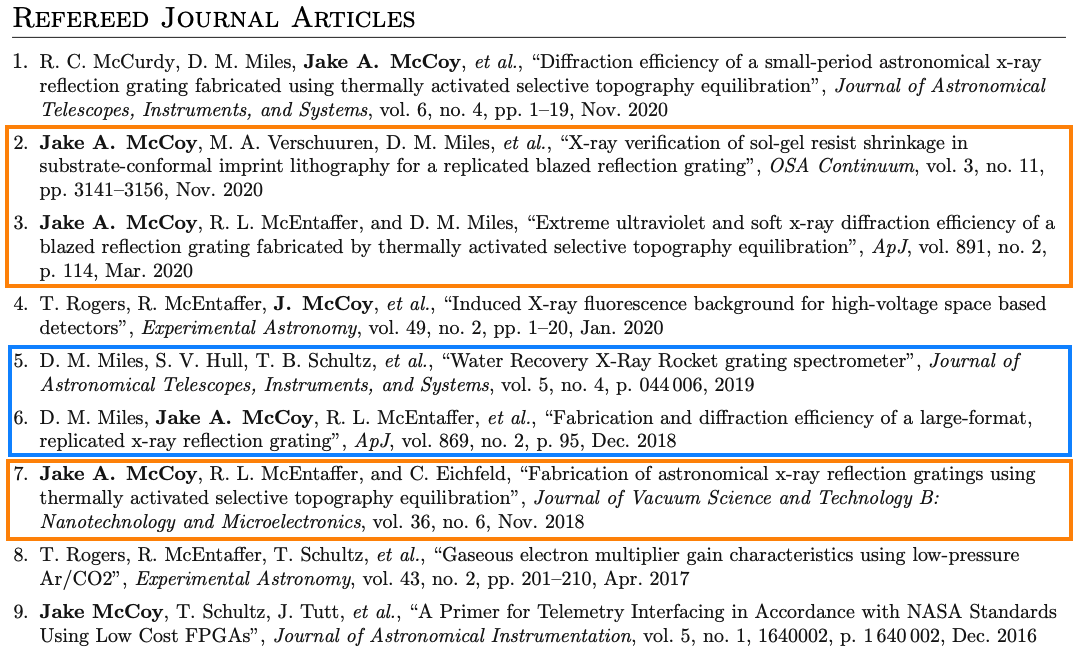
\includegraphics[scale=0.203]{Figures/journal_articles.png}
 \end{figure}
 %\vspace{1mm}
\end{minipage}
\hfill
\begin{minipage}[t]{0.495\linewidth}
\vspace{-0.25mm}
\begin{figure}
 \centering
 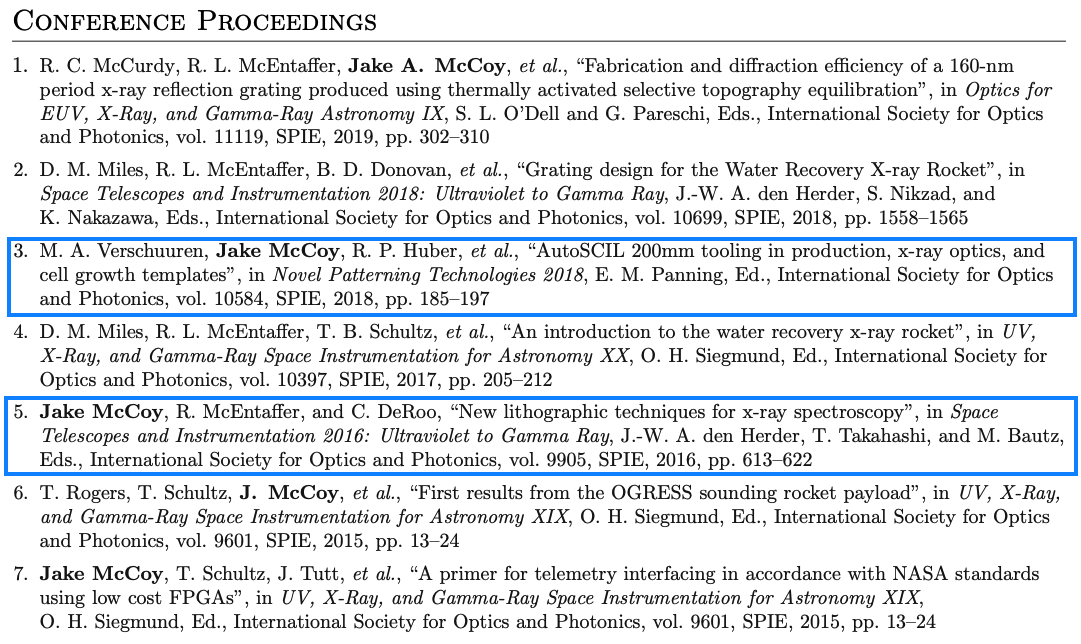
\includegraphics[scale=0.203]{Figures/proceedings.png}
 \end{figure}
 \vspace{5mm}
\end{minipage}
%\vspace{15mm}
\centering {\footnotesize Jargon: \emph{thermally-activated selective topography equilibration (TASTE)}, \emph{substrate-conformal imprint lithography (SCIL)} \newline [Schleunitz, et al.~(2014), Verschuuren~(2010)]}
%{\footnotesize This research was supported by NASA Space Technology Research Fellowships and used resources of the Nanofabrication Laboratory and the Materials Characterization Laboratory at the Penn State Materials Research Institute, Philips SCIL Nanoimprint Solutions and beamline 6.3.2 of the Advanced Light Source, which is a DOE Office of Science User Facility under contract no. DE-AC02-05CH11231.}
\end{frame}

\begin{frame}
 \frametitle{Table of Contents}
 \tableofcontents
\end{frame}

\section{Astrophysical Motivation for Custom Blazed Gratings}

\subsection{Soft X-ray Spectroscopy of Highly-Charged Ions in Circumgalactic \& Intergalactic Media}

\begin{frame}{Astrophysical Motivation for Custom Blazed Gratings}
\begin{minipage}[t]{0.48\linewidth}
 \textbf{Cosmic baryon cycle}
 \begin{itemize}
  \item $\mathcal{Z} > 2$ elements (\emph{metals}) dominated by baryons generated during life cycles of stars with $\gtrapprox 8 M_{\odot}$
  %\item Beyond hydrogen and helium, remaining $\sim \SI{2}{\percent}$ of baryonic matter is dominated by elements generated during life cycles of stars with $\gtrapprox 8 M_{\odot}$ %In quiescent galaxies, 
  %\item Supernovae enrich \emph{interstellar} media (ISM) with atomic nuclei of $\mathcal{Z} \geq 6$ (oxygen, carbon, neon, etc.) %by supernovae %that result from the deaths of these massive stars
  \item CGM \& IGM populated with metals by material outflows from star-forming galaxies, AGN % active galactic nuclei (AGN)
  %\item Expelled material can exist for long time periods as extremely diffuse plasma while portions eventually fall back into ISM %multi-phase? % of host galaxy %and ultimately contributes to star formation, galaxy evolution
  \item \emph{Soft x-ray spectroscopy} has exclusive ability to diagnose highly-ionized portions of CGM \& IGM with $T_{\text{ion}} > \SI{e6}{\kelvin}$ %that are expected to constitute a significant fraction of the total baryon content %in the Universe
 \end{itemize}
 \vspace{5mm}
 \begin{table}[]
 \centering
 \begin{tabular}{@{}lllll@{}} 
 \toprule
 CGM: \emph{circumgalactic media} \\
 (ICM: \emph{intracluster media}) \\ 
 IGM: \emph{intergalactic media} \\
 AGN: \emph{active galactic nuclei} \\
 \bottomrule
 \end{tabular}
 \end{table}
 \end{minipage}
\hfill
\begin{minipage}[t]{0.48\linewidth}
 \begin{figure}
 \centering
 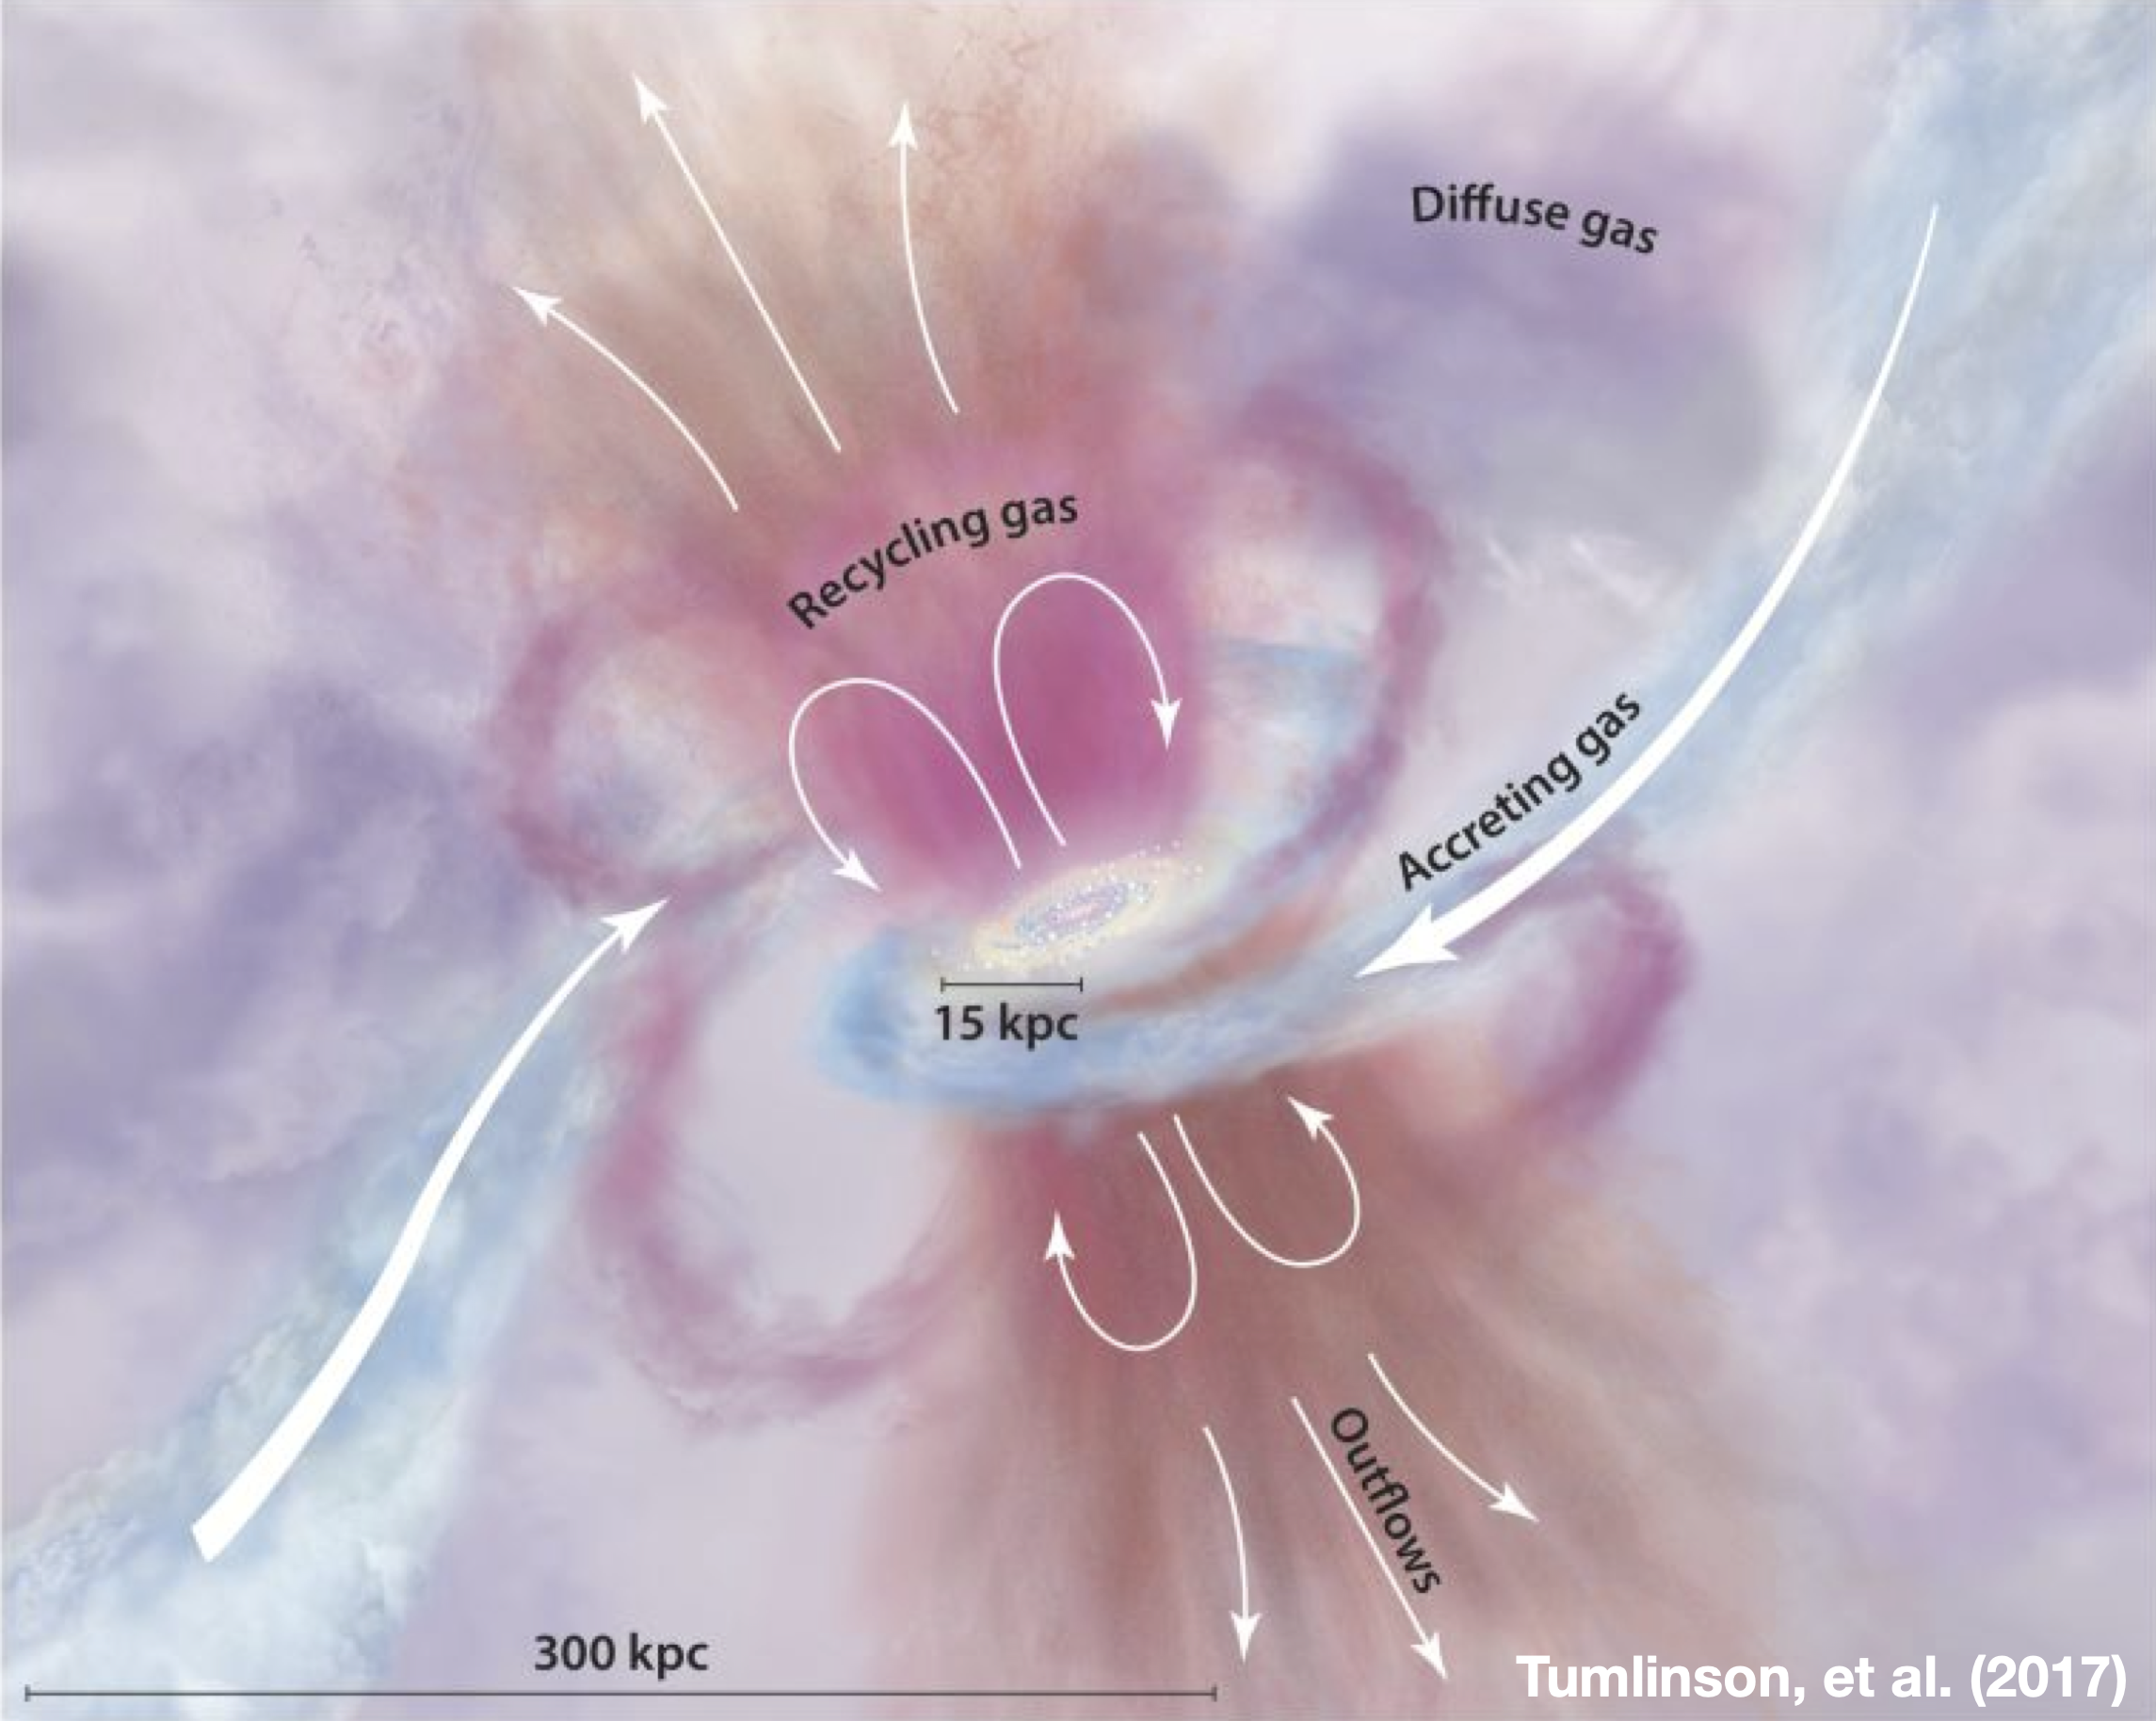
\includegraphics[scale=0.09]{Figures/CGM_edit.png}
 %\caption{Cartoon illustrating how material cycles through a galaxy and its CGM (Tumlinson, et al.~2017)} 
 \end{figure}
 \end{minipage}
\end{frame}


%\begin{frame}{Astrophysical Motivation for Custom Blazed Gratings}
% \begin{minipage}[t]{0.52\linewidth}
% \textbf{Cosmic baryon cycle}
% \begin{itemize}
%  \item Beyond hydrogen and helium, remaining $\sim \SI{2}{\percent}$ of baryonic matter is dominated by elements generated during life cycles of stars with $\gtrapprox 8 M_{\odot}$ %In quiescent galaxies, 
%  \item Supernovae enrich \emph{interstellar} media (ISM) with atomic nuclei of $\mathcal{Z} \geq 6$ (oxygen, carbon, neon, etc.) %by supernovae %that result from the deaths of these massive stars
%  \item \emph{Circumgalactic} and \emph{intergalactic} media (CGM, IGM) are populated with metals by material outflows from active galactic nuclei (AGN)
%  \item Expelled material can exist for long time periods as extremely diffuse plasma while portions eventually fall back into ISM %multi-phase? % of host galaxy %and ultimately contributes to star formation, galaxy evolution
%  \item \emph{Soft x-ray spectroscopy} has exclusive ability to diagnose highly-ionized portions of CGM, IGM with $T_{\text{ion}} > \SI{e6}{\kelvin}$ that are expected to constitute a significant fraction of the total baryon content %in the Universe
% \end{itemize}
% \end{minipage}
%\hfill
%\begin{minipage}[t]{0.45\linewidth}
%\begin{figure}
% \centering
% 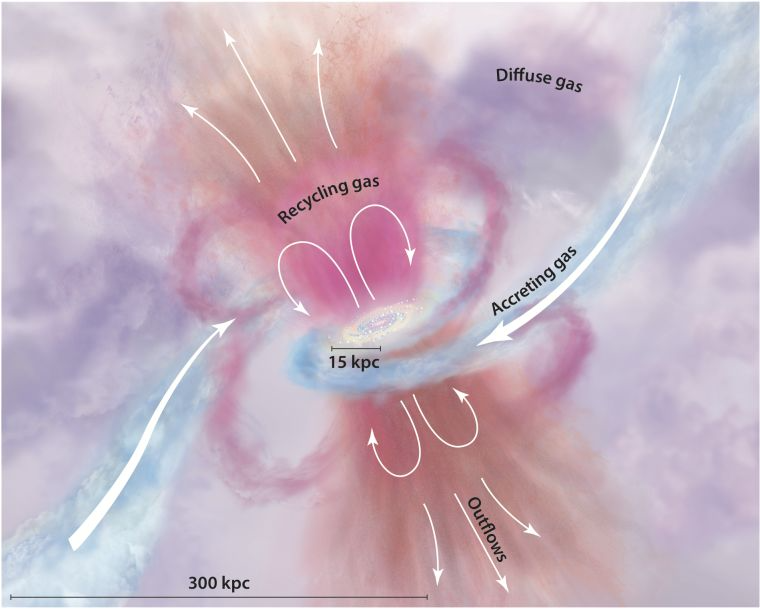
\includegraphics[scale=1.1]{Figures/CGM_Tumlinson.png}
% \caption{Cartoon illustrating how material cycles through an active galaxy and its CGM (Tumlinson, et al.~2017)} 
% \end{figure}
% \end{minipage}
%\end{frame}


\begin{frame}{Astrophysical Motivation for Custom Blazed Gratings}
\begin{minipage}[t]{0.2\linewidth} 
\vspace{3.3mm}
\begin{table}[]
 \centering
 \begin{tabular}{@{}lllll@{}} 
 \toprule
 element ($\mathcal{Z}$) \\ \midrule
 hydrogen ($1$) \\
 helium ($2$) \\
 oxygen ($8$) \\
 carbon ($6$) \\
 neon ($10$) \\
 nitrogen ($7$) \\
 magnesium ($12$) \\
 silicon ($14$) \\
 iron ($26$) \\
 \bottomrule
 \end{tabular}
 \end{table}
{\quad \emph{electric dipole:}}
 \end{minipage}
\begin{minipage}[t]{0.38\linewidth} 
{\quad \textbf{Hydrogen-like ions}}
\begin{table}[]
 \centering
 \begin{tabular}{@{}lllll@{}} 
 \toprule
 ion & transition & spectral band \\ \midrule
 \ion{H}{i} & \SI{10.2}{\electronvolt} & FUV/VUV \\
 \ion{He}{ii} & \SI{40.8}{\electronvolt} & EUV \\
 \ion{O}{viii} & \SI{653.5}{\electronvolt} & soft x-ray \\
 \ion{C}{vi} & \SI{367.5}{\electronvolt} & soft x-ray \\
 \ion{Ne}{x} & \SI{1021.5}{\electronvolt} & soft x-ray \\
 \ion{N}{vii} & \SI{500.2}{\electronvolt} & soft x-ray \\
 \ion{Mg}{xii} & \SI{1471.7}{\electronvolt} & soft x-ray \\
 \ion{Si}{xiv} & \SI{2004.3}{\electronvolt} & soft x-ray \\
 \ion{Fe}{xxvi} & \SI{6952.0}{\electronvolt} & x-ray \\
 \bottomrule
 \end{tabular}
 \end{table}
$\quad 2 p \; {}^2 \! P_{3/2} \leftrightarrow 1 s \; {}^2 \! S_{1/2}$
 \end{minipage}
\begin{minipage}[t]{0.38\linewidth} 
\textbf{\quad Helium-like ions}
\vspace{0.5mm}
\begin{table}[]
 \centering
 \begin{tabular}{@{}lllll@{}} 
 \toprule
 ion & transition & spectral band \\ \midrule
 - & - & - \\
 \ion{He}{ii} & \SI{21.2}{\electronvolt}  & VUV/EUV \\
 \ion{O}{vii} & \SI{573.9}{\electronvolt} & soft x-ray \\
 \ion{C}{v} & \SI{307.9}{\electronvolt} & soft x-ray \\
 \ion{Ne}{ix} & \SI{922.0}{\electronvolt} & soft x-ray \\
 \ion{N}{vi} & \SI{430.7}{\electronvolt} & soft x-ray \\
 \ion{Mg}{xi} & \SI{1352.2}{\electronvolt} & soft x-ray \\
 \ion{Si}{xiii} & \SI{1865.0}{\electronvolt} & soft x-ray \\
 \ion{Fe}{xxv} & \SI{6700.4}{\electronvolt} & x-ray \\
 \bottomrule
 \end{tabular}
 \end{table}
 $\quad 1s \, 2 p \; {}^1 \! P_{1} \leftrightarrow 1 s^2 \; {}^1 \! S_{0}$ {\tiny \quad (data obtained from AtomDB)}
 \end{minipage}
\vspace{1mm}
 \begin{itemize}
  \item \ce{H}-like \& \ce{He}-like ions - most extreme charge states
  \item Oxygen is most abundant $\mathcal{Z} > 2$ element
  \item Electric-dipole transitions (\emph{resonance lines}) have largest transition rates, appear strongest in spectrum
 \end{itemize}
\end{frame}

\begin{frame}{Astrophysical Motivation for Custom Blazed Gratings}
\begin{minipage}[t]{0.48\linewidth} 
\begin{figure}
 \centering
 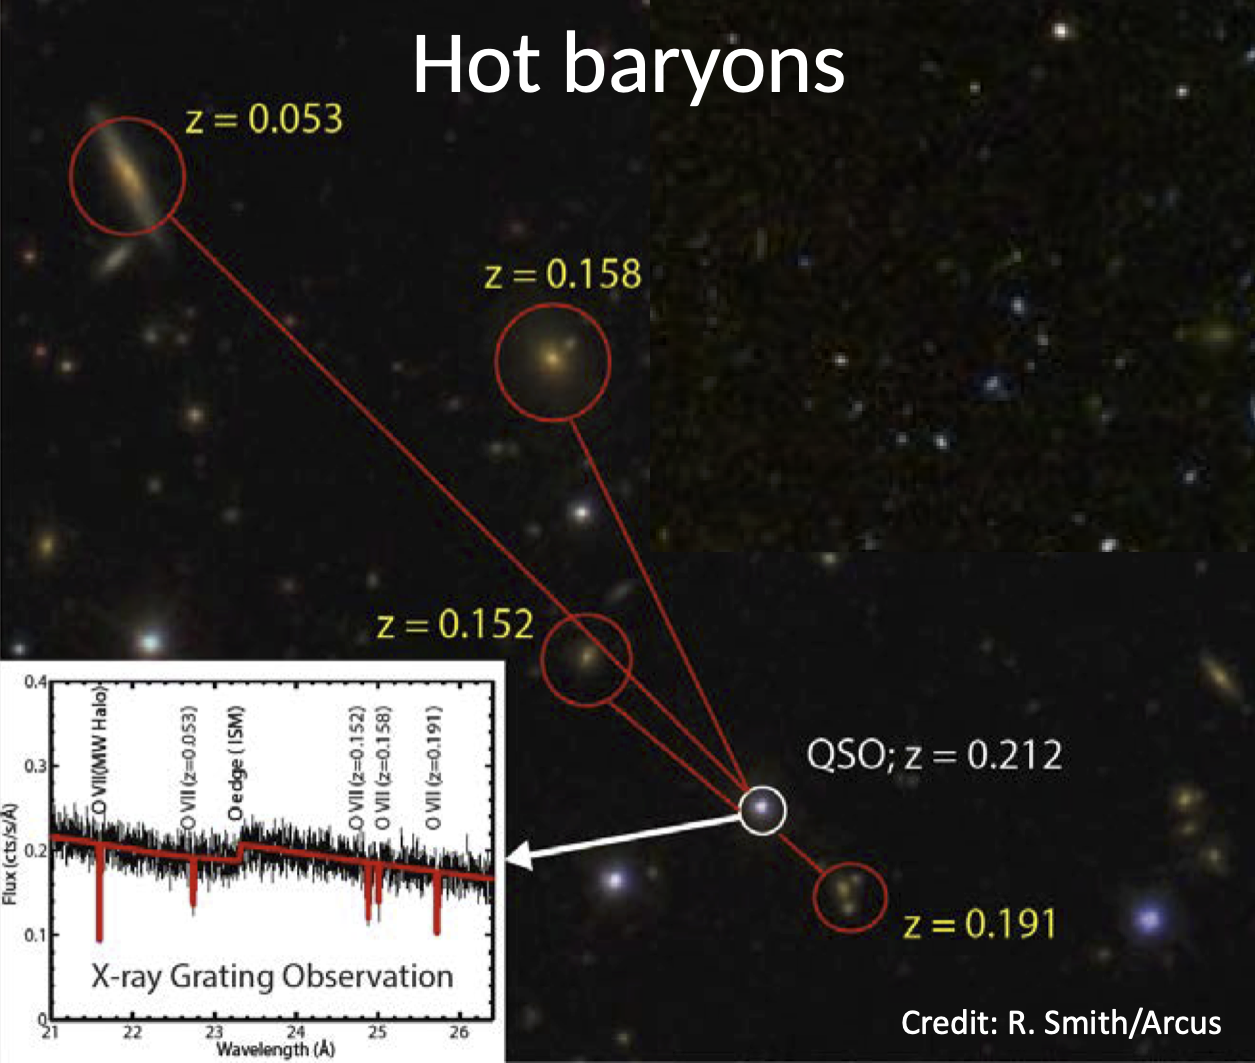
\includegraphics[scale=0.16]{Figures/hot_baryons.png}
 %\caption{Cartoon illustrating how material cycles through an active galaxy and its CGM (Tumlinson, et al.~2017)} 
 \end{figure}
\end{minipage}
\hfill
\begin{minipage}[t]{0.48\linewidth} 
\vspace{5mm}
 \begin{itemize}
  \item The \emph{emission measure}, $\text{EM} \equiv \int n_e n_{\text{ion}} \dd[3]{\mathbold{r}}$, is very low in diffuse CGM, IGM
  \item Absorption spectroscopy using AGN continua beneficial for detecting weak spectral lines
  %\begin{itemize}
  %  \item[$\implies$] Up-scattered UV radiation from accretion disk 
  %\end{itemize}
  \item Measure spectral lines at various redshifts, $z$, correlate with intercepting galaxies
  %\item[$\implies$] \emph{Motivate why gratings are instrument of choice for sensitive spectroscopy}
 \end{itemize}
\end{minipage}
\end{frame}

\begin{frame}{Astrophysical Motivation for Custom Blazed Gratings}
\begin{minipage}[t]{0.42\linewidth}
\vspace*{-5mm}
\begin{figure}
 \centering
 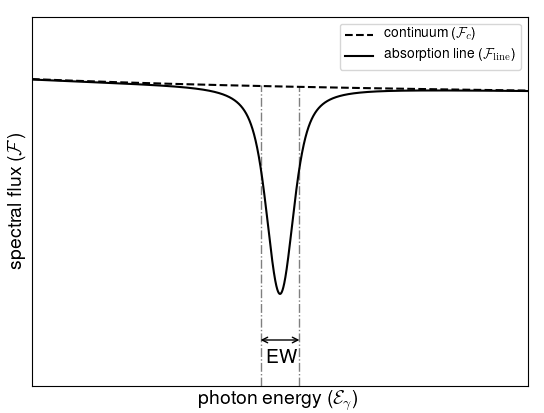
\includegraphics[scale=0.45]{Figures/line_test.png}
 \caption{Voigt profile of absorption line, $\mathcal{F}_{\text{line}}$, with underlying AGN continuum: $\mathcal{F}_c \propto \mathcal{E}_{\gamma}^{-0.7}$ \vspace*{-5mm}}
 \end{figure}
{\vspace*{3mm} {\quad \footnotesize \emph{equivalent width:}} $\text{EW} \equiv \int \left(  \frac{\mathcal{F}_c - \mathcal{F}_{\text{line}}}{\mathcal{F}_c} \right) \dd{\mathcal{E}_{\gamma}}$} %\\ 
%{\vspace*{1mm} {\quad \ \ \ \footnotesize \emph{in terms of } $\lambda$:} $W_{\lambda} = \frac{\lambda^2}{\SI{1240}{\electronvolt\nm}} W_{\gamma}$}
 \end{minipage}
\hfill
\begin{minipage}[t]{0.55\linewidth} 
 \textbf{Energy-dispersive spectroscopy} ($\mathscr{R} = \mathcal{E}_{\gamma} / \Delta \mathcal{E}_{\gamma}$)
  \begin{itemize}
  \item unresolved line: $F_{\text{line}} \equiv \left[ \mathcal{F}_c - \mathcal{F}_{\text{line}} \right] \Delta \mathcal{E}_{\gamma}$ %with $N_{\text{line}} = F_{\text{line}} A_{\text{col}} t_{\text{obs}}$ and $N_{\text{tot}} = N_c - N_{\text{line}}$ %for given observation
  \item photons: $N_{\text{line}} = F_{\text{line}} A_{\text{col}} t_{\text{obs}}$ with $N_{\text{tot}} = N_c - N_{\text{line}}$ 
 \end{itemize}
 \vspace{-2mm}
  \begin{block}{\footnotesize \emph{Equivalent width of weak, unresolved spectral line}}
   \centering
    $\text{EW} = \frac{F_{\text{line}}}{\mathcal{F}_c} \approx \tau^{\text{ion}}_{\gamma} \Delta \mathcal{E}_{\gamma} \ \ \text{with} \ \ \tau^{\text{ion}}_{\gamma} \equiv \sigma^{\text{ion}}_{\gamma} \mathcal{N}^{\text{ion}}_{\gamma} \ \ (\text{\emph{optical depth}})$ %\mathcal{N}^{\text{ion}}_{\gamma} = \int n^{\text{ion}}_{\gamma} \dd{\ell}%%$W_{\gamma} \equiv \int \frac{\mathcal{F}_c - \mathcal{F}_{\text{line}}}{\mathcal{F}_c} \dd{\mathcal{E}_{\gamma}} = \int \left(  1 - \mathrm{e}^{- \tau^{\text{ion}}_{\gamma}} \right) \dd{\mathcal{E}_{\gamma}} \approx \int \tau^{\text{ion}}_{\gamma} \dd{\mathcal{E}_{\gamma}}$
  \end{block}
  \vspace{-2mm}
 \begin{itemize}
  \item $\text{EW}$ yields $\tau^{\text{ion}}_{\gamma}$ $\implies$ ion density can be inferred%for specific ion so that density of ionic species in plasma can be inferred 
  \item Detection depends on signal-to-noise: $\mathcal{S} = N_{\text{line}} / \sqrt{N_{\text{tot}}}$ with $N_{\text{tot}} \approx N_c = N_{\text{line}} \Delta \mathcal{E}_{\gamma} / \text{EW}$ %for very small EW %(for $\text{EW} \ll \Delta \mathcal{E}_{\gamma}$)
 \end{itemize}
  \vspace{-2mm}
   \begin{block}{\footnotesize \emph{Instrument figure of merit for weak absorption line}}
   \centering
    $\text{FOM}_{\text{weak}} \propto \frac{\mathcal{S}}{\sqrt{F_{\text{line}}t_{\text{obs}}}} \approx \sqrt{\frac{A_{\text{col}} \text{EW}}{\Delta \mathcal{E}_{\gamma}}} \propto \sqrt{A_{\text{col}} \mathscr{R}}$ 
  \end{block}
  \vspace{-1mm}
  \centering {\textbf{High spectral resolving power \& large collecting area both required for sensitive spectroscopy}}
 \end{minipage}
\end{frame}

\begin{frame}{Astrophysical Motivation for Custom Blazed Gratings}
\begin{minipage}[t]{0.72\linewidth}
\begin{figure}
 \centering
 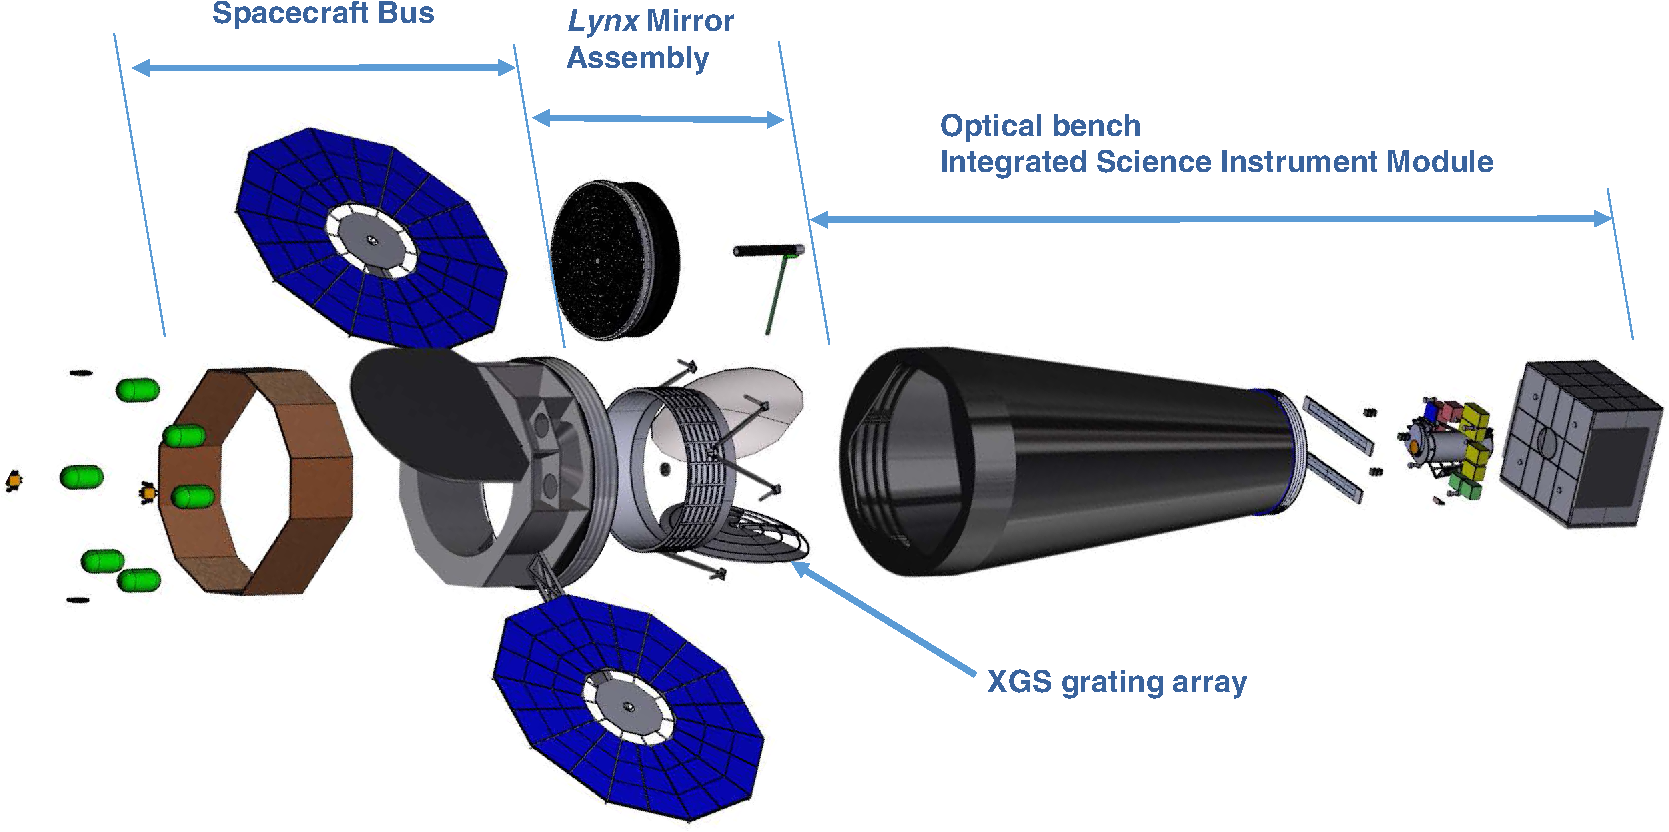
\includegraphics[scale=0.25]{Figures/JATIS_5_2_021002_f004.png}
 \caption{An exploded view of the \emph{Lynx X-ray Observatory} (McEntaffer~2019)}
 \end{figure}
 \end{minipage}
\begin{minipage}[t]{0.26\linewidth}
 \textbf{\emph{Lynx} spectroscopy}
 \begin{itemize}
  \item \emph{Lynx X-ray Microcalorimeter (LXM)}
  \begin{itemize}
    %\item Measure photon energy ($\mathcal{E}_{\gamma}$)
    \item[$\square$] $\mathscr{R} = \mathcal{E}_{\gamma} / \Delta \mathcal{E}_{\gamma}$
  \end{itemize}
  \item \emph{X-ray Grating Spectrometer (XGS)}
    \begin{itemize}
    %\item Measure $\lambda$
    \item[$\square$] $\mathscr{R} = \lambda / \Delta \lambda$
  \end{itemize}
  \item Compare \emph{LXM} and \emph{XGS} for spectroscopy of CGM \& IGM %highly-ionized plasmas in
  \item \underline{\emph{X-ray reflection gratings}} \& \emph{critical-angle transmission gratings} considered for \emph{XGS}
 \end{itemize}
 \end{minipage}
 \vspace{1mm}
 \centering {\footnotesize \emph{cf.\@} Gaskin, et al.~(2019)}
\end{frame}

\begin{frame}{Astrophysical Motivation for Custom Blazed Gratings}
 \begin{minipage}[t]{0.55\linewidth}
 \textbf{The need for next-generation x-ray gratings}
 \begin{itemize}
  \item \ion{O}{viii} and \ion{O}{vii} important for absorption studies
  \begin{itemize}
    \item High $\sqrt{A_{\text{col}} \mathscr{R}}$ required for $\mathcal{E}_{\gamma} \lessapprox \SI{650}{\electronvolt} / (1 + z)$
    \item $\mathscr{R} \gtrapprox 5000$ desirable for resolving thermally-broadened oxygen line with $T_{\text{ion}} > \SI{e6}{\kelvin}$ 
  \end{itemize}
  %\item A next-generation grating spectrometer is required for the detection of weak absorption lines in CGM, IGM
 \end{itemize}
  %\vspace{-2mm}
  %\begin{block}{\footnotesize \emph{Thermally-broadened oxygen line}}
  % \centering
  %  $\mathscr{R}_D \equiv \frac{\mathcal{E}'_{\gamma}}{\Delta \mathcal{E}_D} = \frac{1}{1 + z} \sqrt{\frac{m_{\text{ion}} c_0^2}{2 k_{\mathcal{B}} T_{\text{ion}}}} \gtrapprox 5000 \ \ \text{with} \ \ T_{\text{ion}} > \SI{e6}{\kelvin}$ 
  %\end{block}
  %%\vspace{-2mm}
 \begin{itemize}
  \item \emph{LXM} baselines $A_{\text{col}} \approx \SI{1000}{\cm\squared}$ and $\Delta \mathcal{E}_{\gamma} \approx \SI{3}{\electronvolt}$ 
  \begin{itemize}
    \item $\mathscr{R} = \mathcal{E}_{\gamma} / \Delta \mathcal{E}_{\gamma} \lessapprox 350$ for $\mathcal{E}_{\gamma} \lessapprox \SI{1}{\kilo\electronvolt}$
    %\item Alternative: $\lambda$-dispersive spectroscopy ($\mathscr{R} = \lambda / \Delta \lambda$)
  \end{itemize} 
  \item \emph{XGS} baselines $A_{\text{col}} \gtrapprox \SI{4000}{\cm\squared}$ and $\Delta \lambda \approx \SI{4}{\milli\angstrom}$
  \begin{itemize}
    \item $\mathscr{R} = \lambda / \Delta \lambda \gtrapprox 5000$ for $n \lambda \gtrapprox \SI{2}{\nm}$ %($\mathcal{E}_{\gamma} \lessapprox \SI{620}{\electronvolt}$) \vspace{1mm}
    \item $\text{FOM}_{\text{weak}} \lessapprox 8$ that of \emph{LXM}, $\lessapprox 20$ that of \emph{XMM-Newton}
  \end{itemize}
 \end{itemize}
 \vspace{2mm}
 \begin{exampleblock}{\emph{Lynx} science goal}
  \centering {Probe density of CGM, IGM through measuring $\text{EW} \gtrapprox \SI{1}{\milli\angstrom}$ for many AGN-absorbing systems, correlating measured $z$ with those of intercepting galaxies}
  \end{exampleblock}
 \end{minipage}
\hfill
\begin{minipage}[t]{0.42\linewidth}
\vspace{-2mm}
\begin{figure}
 \centering
 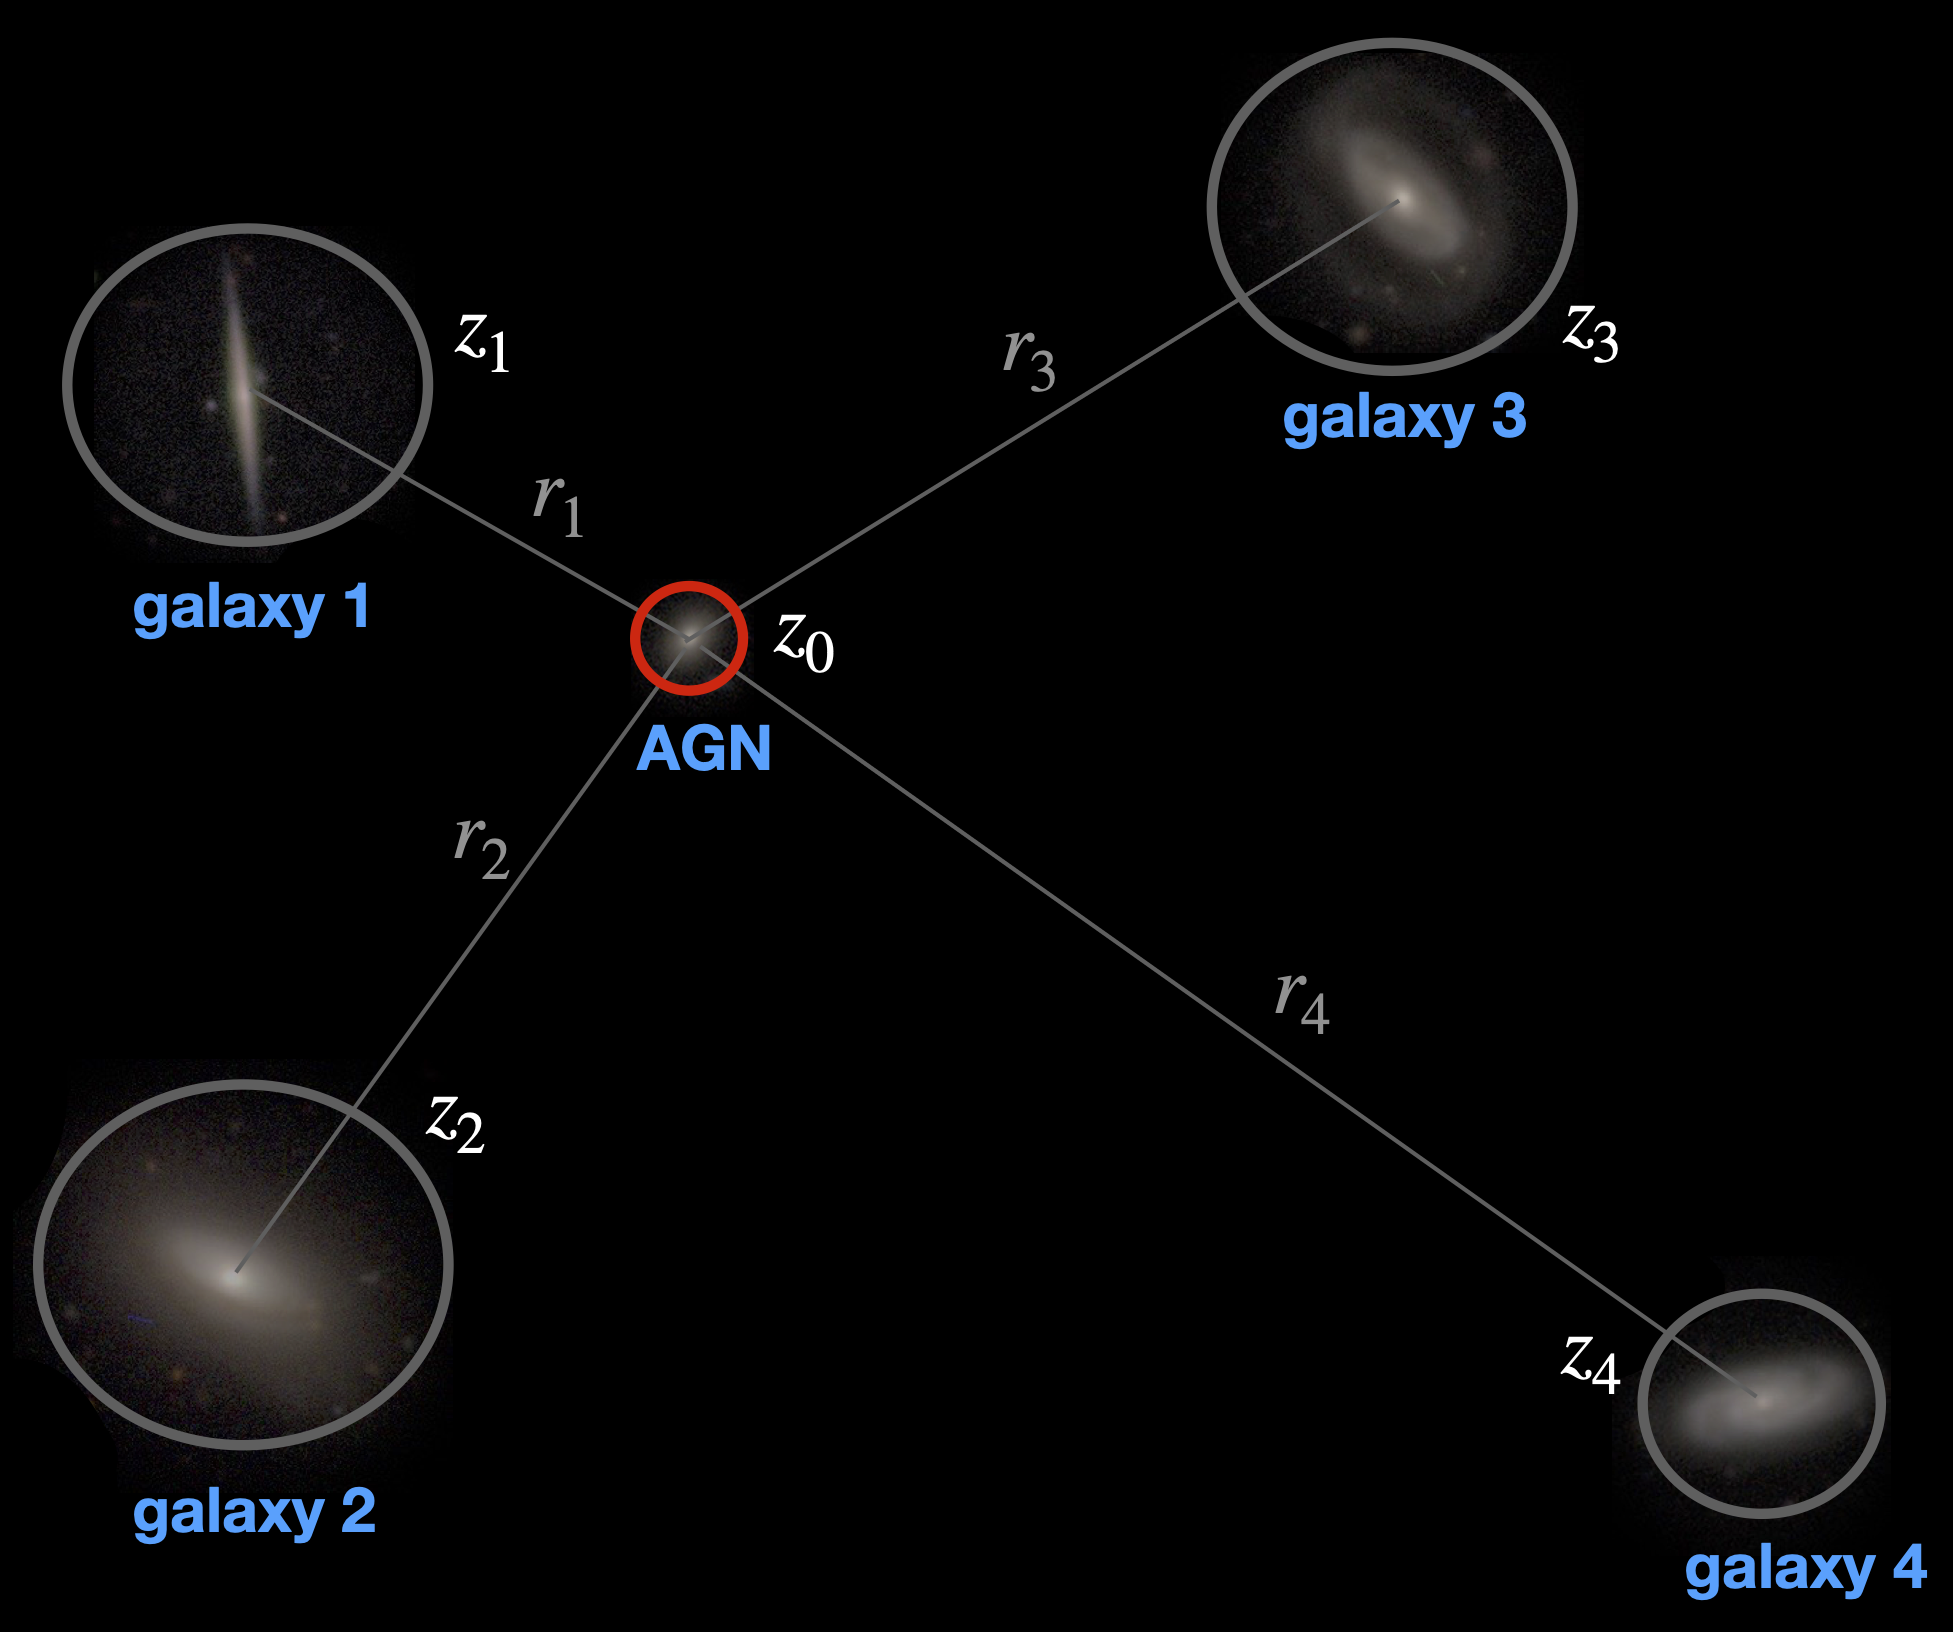
\includegraphics[scale=0.2]{Figures/galaxy_field.png}
 \caption{Cartoon of an AGN at a redshift $z_0$ with four galaxies at smaller redshifts $z_i$ (for $i=$ \numrange{1}{4}) in the foreground for absorption spectroscopy} %The result is a spectrum featuring prominent absorption lines from each intervening galaxy with centroids that depend on $z_i$ and equivalent widths that give an indication of plasma density, which in turn depends on $r_i$.
 \end{figure}
 {\vspace*{-6mm} \tiny (Depicted galaxies are optical images obtained from \textsc{Galaxy Zoo})}
 \end{minipage}
\end{frame}


\subsection{Technological Development of X-ray Reflection Gratings}

\begin{frame}{Astrophysical Motivation for Custom Blazed Gratings}
\begin{minipage}[t]{0.5\linewidth}
\textbf{Main technological challenges of grating fabrication}  
\begin{enumerate}
    \item Producing a master grating with a sawtooth surface-relief profile that enables 
    \begin{itemize}
        \item Total absolute diffraction efficiency $> \SI{40}{\percent}$ % in the soft x-ray exceeding \SI{40}{\percent} %, and 
        \item $\mathscr{R} \gtrapprox 5000$ in a Wolter-I telescope (variable-line-space groove layout)
    \end{itemize}
    %and additionally,  
    \item Mass-replicating thousands of blazed gratings to populate modular grating arrays %for a soft x-ray spectrometer such as the \emph{XGS}. 
\end{enumerate}
\begin{figure}
 \centering
 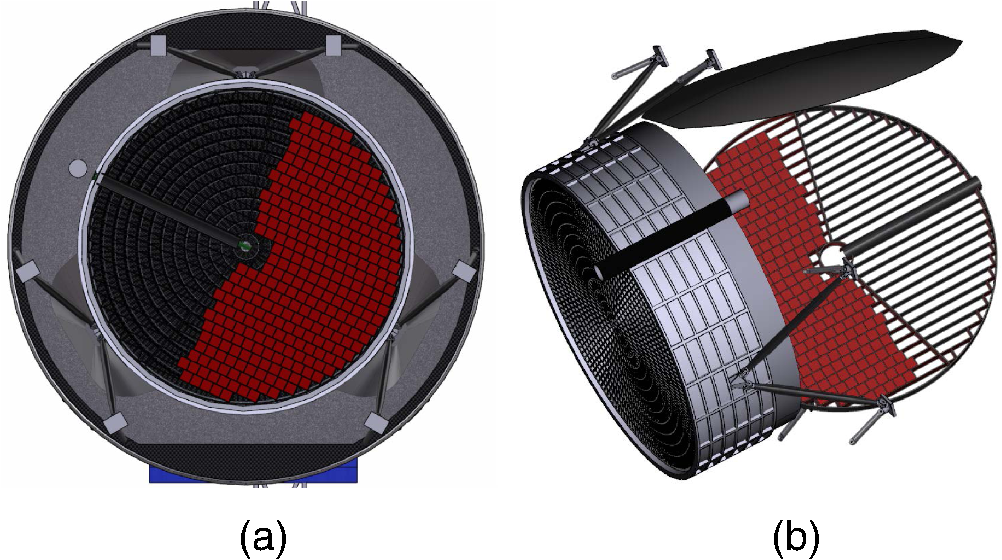
\includegraphics[scale=0.2]{Figures/JATIS_5_2_021002_f008.png}
 \caption{Modular reflection grating arrays (red) for \emph{XGS} relative to \emph{Lynx Mirror Assembly} (McEntaffer~2019)}
 \end{figure}
\end{minipage}
\hfill
\begin{minipage}[t]{0.46\linewidth}
\vspace{-5mm}
\begin{figure}
 \centering
 \includegraphics[scale=0.35]{Figures/diffraction_arc30.mps}
 \vspace{-2mm}
 \caption{Reflection grating geometry for conical diffraction with radial groove layout (not to scale)}
 \end{figure}
 \end{minipage}
\end{frame}

\begin{frame}{Astrophysical Motivation for Custom Blazed Gratings}
\begin{minipage}[t]{0.55\linewidth}
 \textbf{X-ray reflection grating fabrication}
 \begin{enumerate}
  \item \underline{Mechanical ruling engine}
  \begin{itemize}
    \item Diamond-tip burnishing%Classical manufacture method: diamond-tip burnishing
    \item 182 replicas cast in resin for \emph{XMM-Newton RGS}
  \end{itemize}
  \item \underline{Holographic recording} %(interference lithography)
  %\vspace{-1mm}
  \begin{itemize}
    \item Generate sinusoid in \emph{photoresist} following wet development
    \item Produces parallel or curved groove layout
    %\item $d$ limited by wavelength of recording laser
  \end{itemize}
  \item \underline{Electron-beam lithography (EBL)}
  \begin{itemize}
    \item Pattern laminar structure in \emph{polymeric resist} using high-energy electrons, wet development %such as PMMA %\footnote{(\ce{C5H8O2})$_n$} 
    \item Couple with \emph{crystallographic etching} to realize sawtooth %topography %(\emph{next slide})
    %\item Carried out at Penn State Nanofab 
    \item[$\square$] {\footnotesize Franke, et al.~(1997), McEntaffer et al.~(2013), Miles, et al.~(2018)}
  \end{itemize}
  %\item PMMA (\ce{C5H8O2})$_n$
  \item \underline{Nanoimprint lithography (NIL)}
  \begin{itemize}
    \item Use silicon master to imprint replicas in resist %thermal or UV-curable resist
    \item \textsc{Nanonex} UV-NIL pursued previously %for x-ray reflection gratings
    \item[$\square$] {\footnotesize Chang~(2003,2004), McEntaffer et al.~(2013), Miles, et al.~(2018)}
  \end{itemize}
 \end{enumerate}
 \end{minipage}
\hfill
\begin{minipage}[t]{0.42\linewidth}
\vspace{-4mm}
\begin{figure}
 \centering
 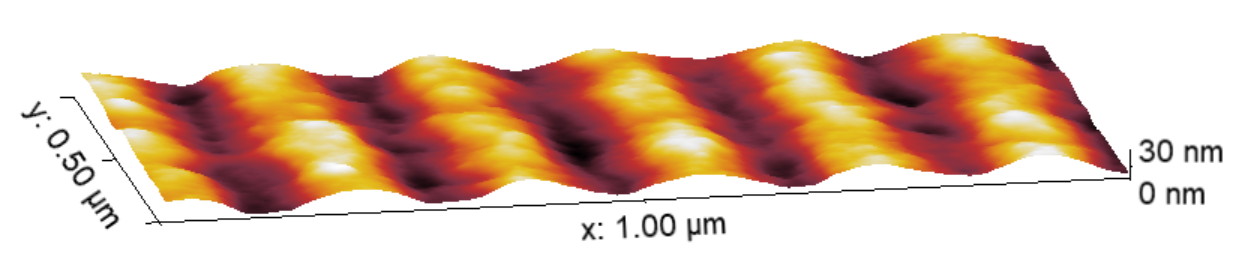
\includegraphics[scale=0.29]{Figures/OGRESS_capture.PNG}
 \caption{\emph{Atomic force micrograph (AFM)} of sinusoidal grating used for sounding rockets (\textsc{Jobin Yvon} )}\label{fig:OGRESS_AFM}
 \end{figure}
 \vspace{-4mm}
 \begin{figure} 
 \centering
 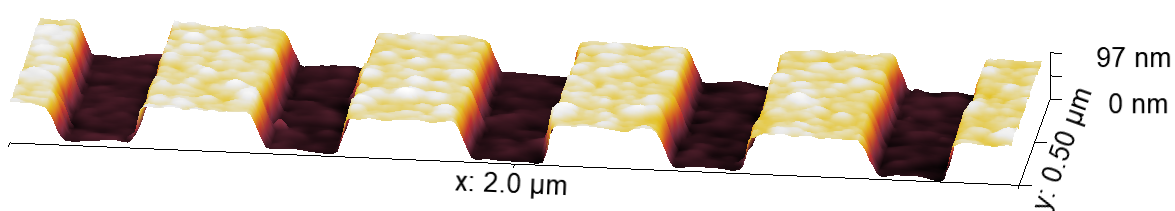
\includegraphics[scale=0.2]{Figures/laminar_amorphous_AFM.PNG}
 \caption{AFM of laminar grating dry etched in amorphous silicon (Penn State Nanofab)}\label{fig:laminar_AFM}
 \end{figure}
 \vspace{-4mm}
 \begin{figure} 
 \centering
 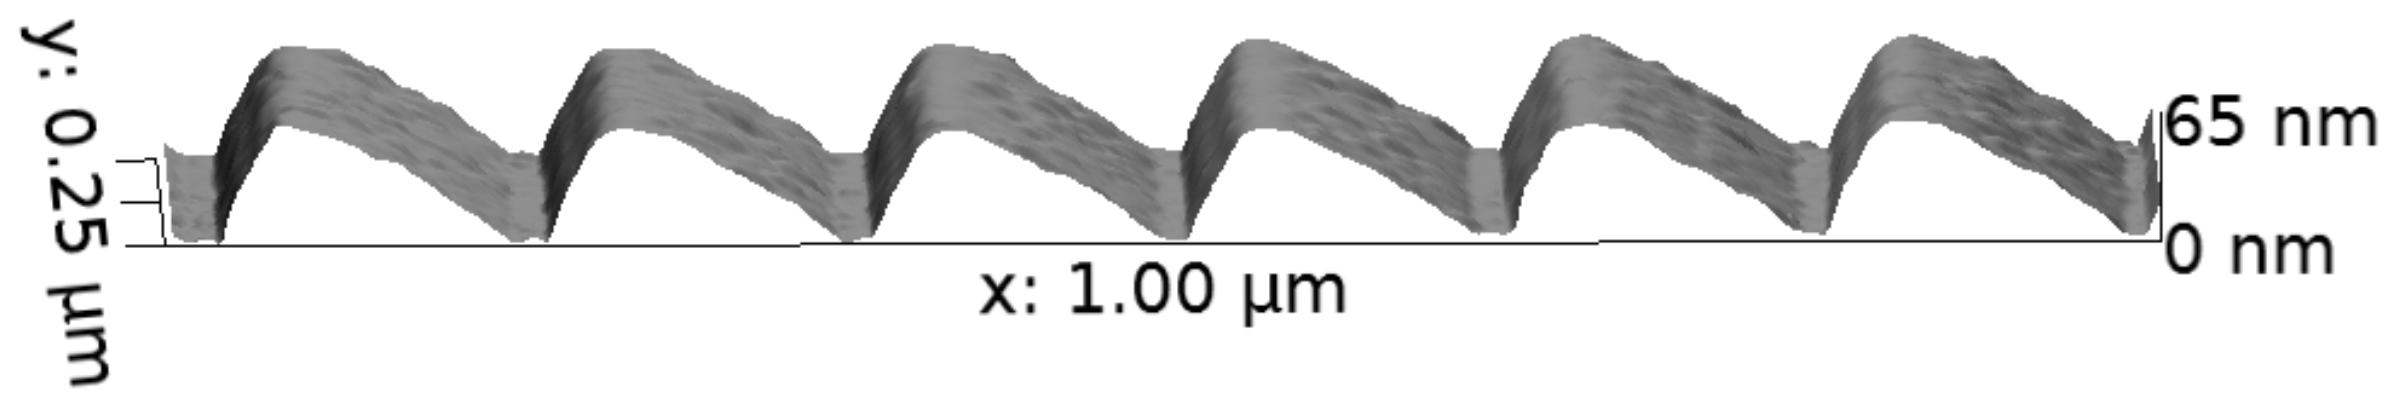
\includegraphics[scale=0.15]{Figures/UV-NIL_AFM.PNG}
 \caption{AFM of blazed grating fabricated by UV-NIL from \ce{KOH}-etched master (Image credit: T.\ Tighe)}\label{fig:uv_nil_AFM} 
 \end{figure}
 \end{minipage}
 %\vspace{-10mm}
\end{frame}

\begin{frame}{Astrophysical Motivation for Custom Blazed Gratings}
\begin{minipage}[t]{0.48\linewidth}
\begin{figure} 
 \centering
 \includegraphics[scale=0.51]{Figures/master_fab1.mps}
 \includegraphics[scale=0.51]{Figures/master_fab2.mps}
 \includegraphics[scale=0.51]{Figures/master_fab3.mps}
 \includegraphics[scale=0.51]{Figures/master_fab4.mps}
 \includegraphics[scale=0.51]{Figures/master_fab5.mps}
 \includegraphics[scale=0.51]{Figures/master_fab6.mps}
 \includegraphics[scale=0.51]{Figures/master_fab7.mps}
 \includegraphics[scale=0.51]{Figures/master_fab8.mps}
 \caption{Outline of fabrication recipe for crystallographic etching in $\langle 311 \rangle$-oriented silicon wafer using EBL}
 \end{figure}
 \vspace{-3mm}
 \centering{\footnotesize \emph{cf.\@} Miles, McCoy, McEntaffer, et al.~(2018)}
 \end{minipage}
\hfill
\begin{minipage}[t]{0.48\linewidth}
\begin{figure}
 \centering
 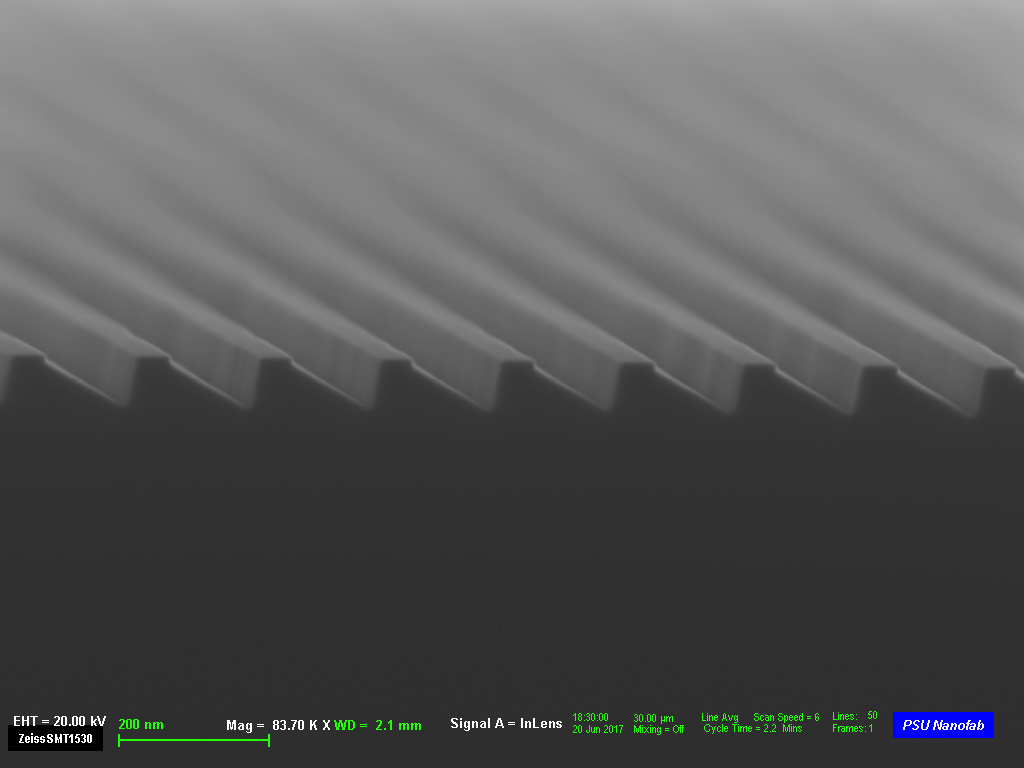
\includegraphics[scale=0.2]{Figures/master_04.jpg}
 \caption{Field emission scanning electron micrograph (FESEM) of $d \lessapprox \SI{160}{\nm}$ \ce{KOH}-etched grating}\label{fig:master_grating_SEM} %viewed edge-on (taken with \textsc{Zeiss Leo 1530} at Penn State Nanofab)
 \end{figure}
 \end{minipage}
\end{frame}

\begin{frame}{Astrophysical Motivation for Custom Blazed Gratings}
\begin{minipage}[t]{0.45\linewidth}
\begin{figure} 
 \centering
 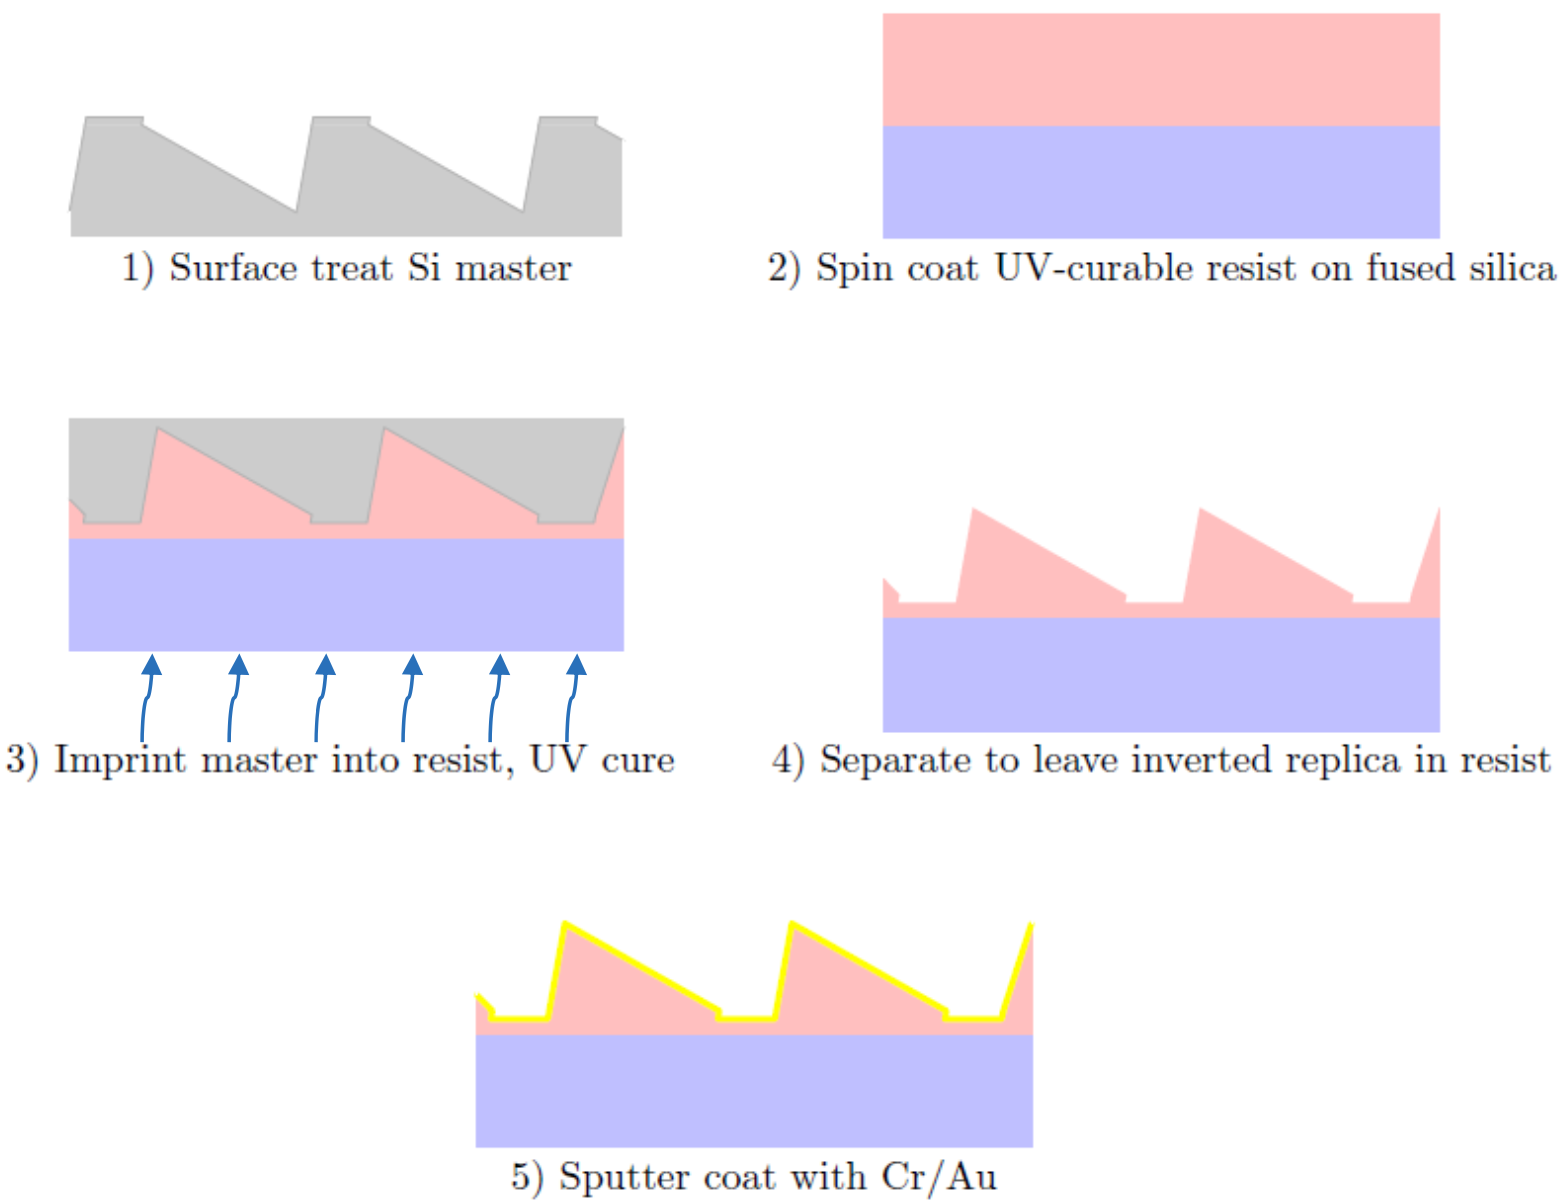
\includegraphics[scale=0.25]{Figures/UV-NIL.PNG}
 \caption{Outline of UV-NIL grating replication process using \ce{KOH}-etched as stamp}\label{fig:uv_nil} 
 \end{figure}
  \vspace{-3mm}
  \centering{\footnotesize \emph{cf.\@} Miles, et al.~(2018)}
 \end{minipage}
\hfill
\begin{minipage}[t]{0.52\linewidth}
\begin{figure} 
 \centering
 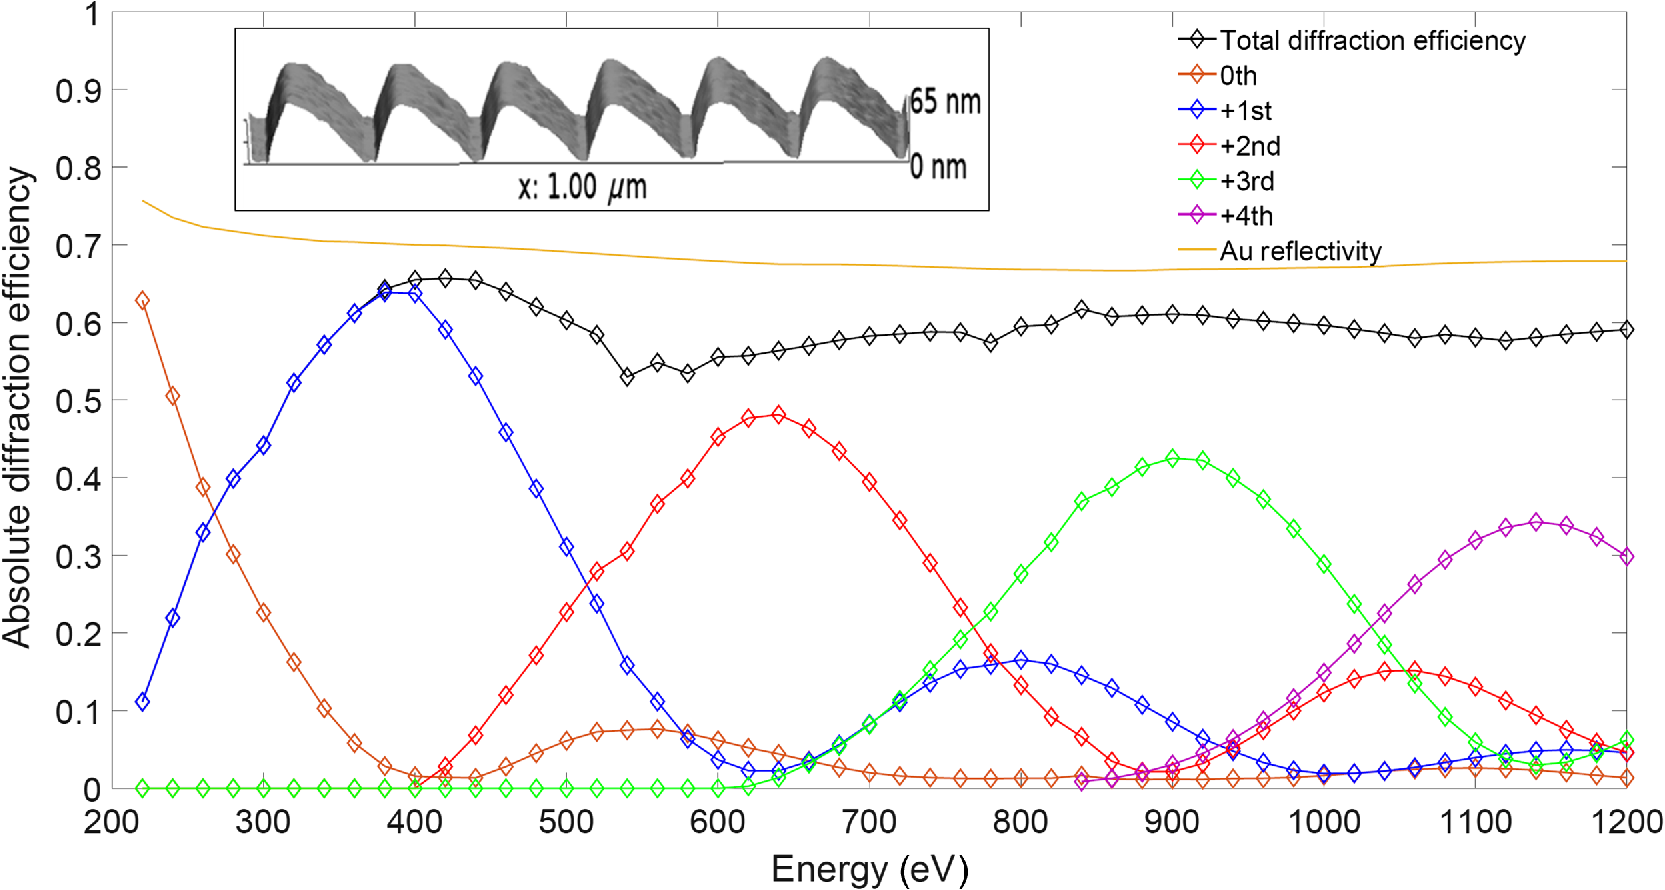
\includegraphics[scale=0.18]{Figures/JATIS_5_2_021002_f002.png}
 \caption{Measured diffraction efficiency of gold-coated UV-NIL imprint meets \emph{Lynx} sensitivity requirements (Miles, et al.~2018)}
 \end{figure}
 \vspace{-5mm}
  \begin{exampleblock}{\emph{Lynx XGS} requirement}
  \centering
  Total diffraction efficiency $> \SI{40}{\percent}$ in the soft x-ray
  \end{exampleblock}
 \end{minipage}
\end{frame}

\begin{frame}{Astrophysical Motivation for Custom Blazed Gratings}
\begin{minipage}[t]{0.38\linewidth}
\vspace{-4mm}
\begin{figure}
 \centering
 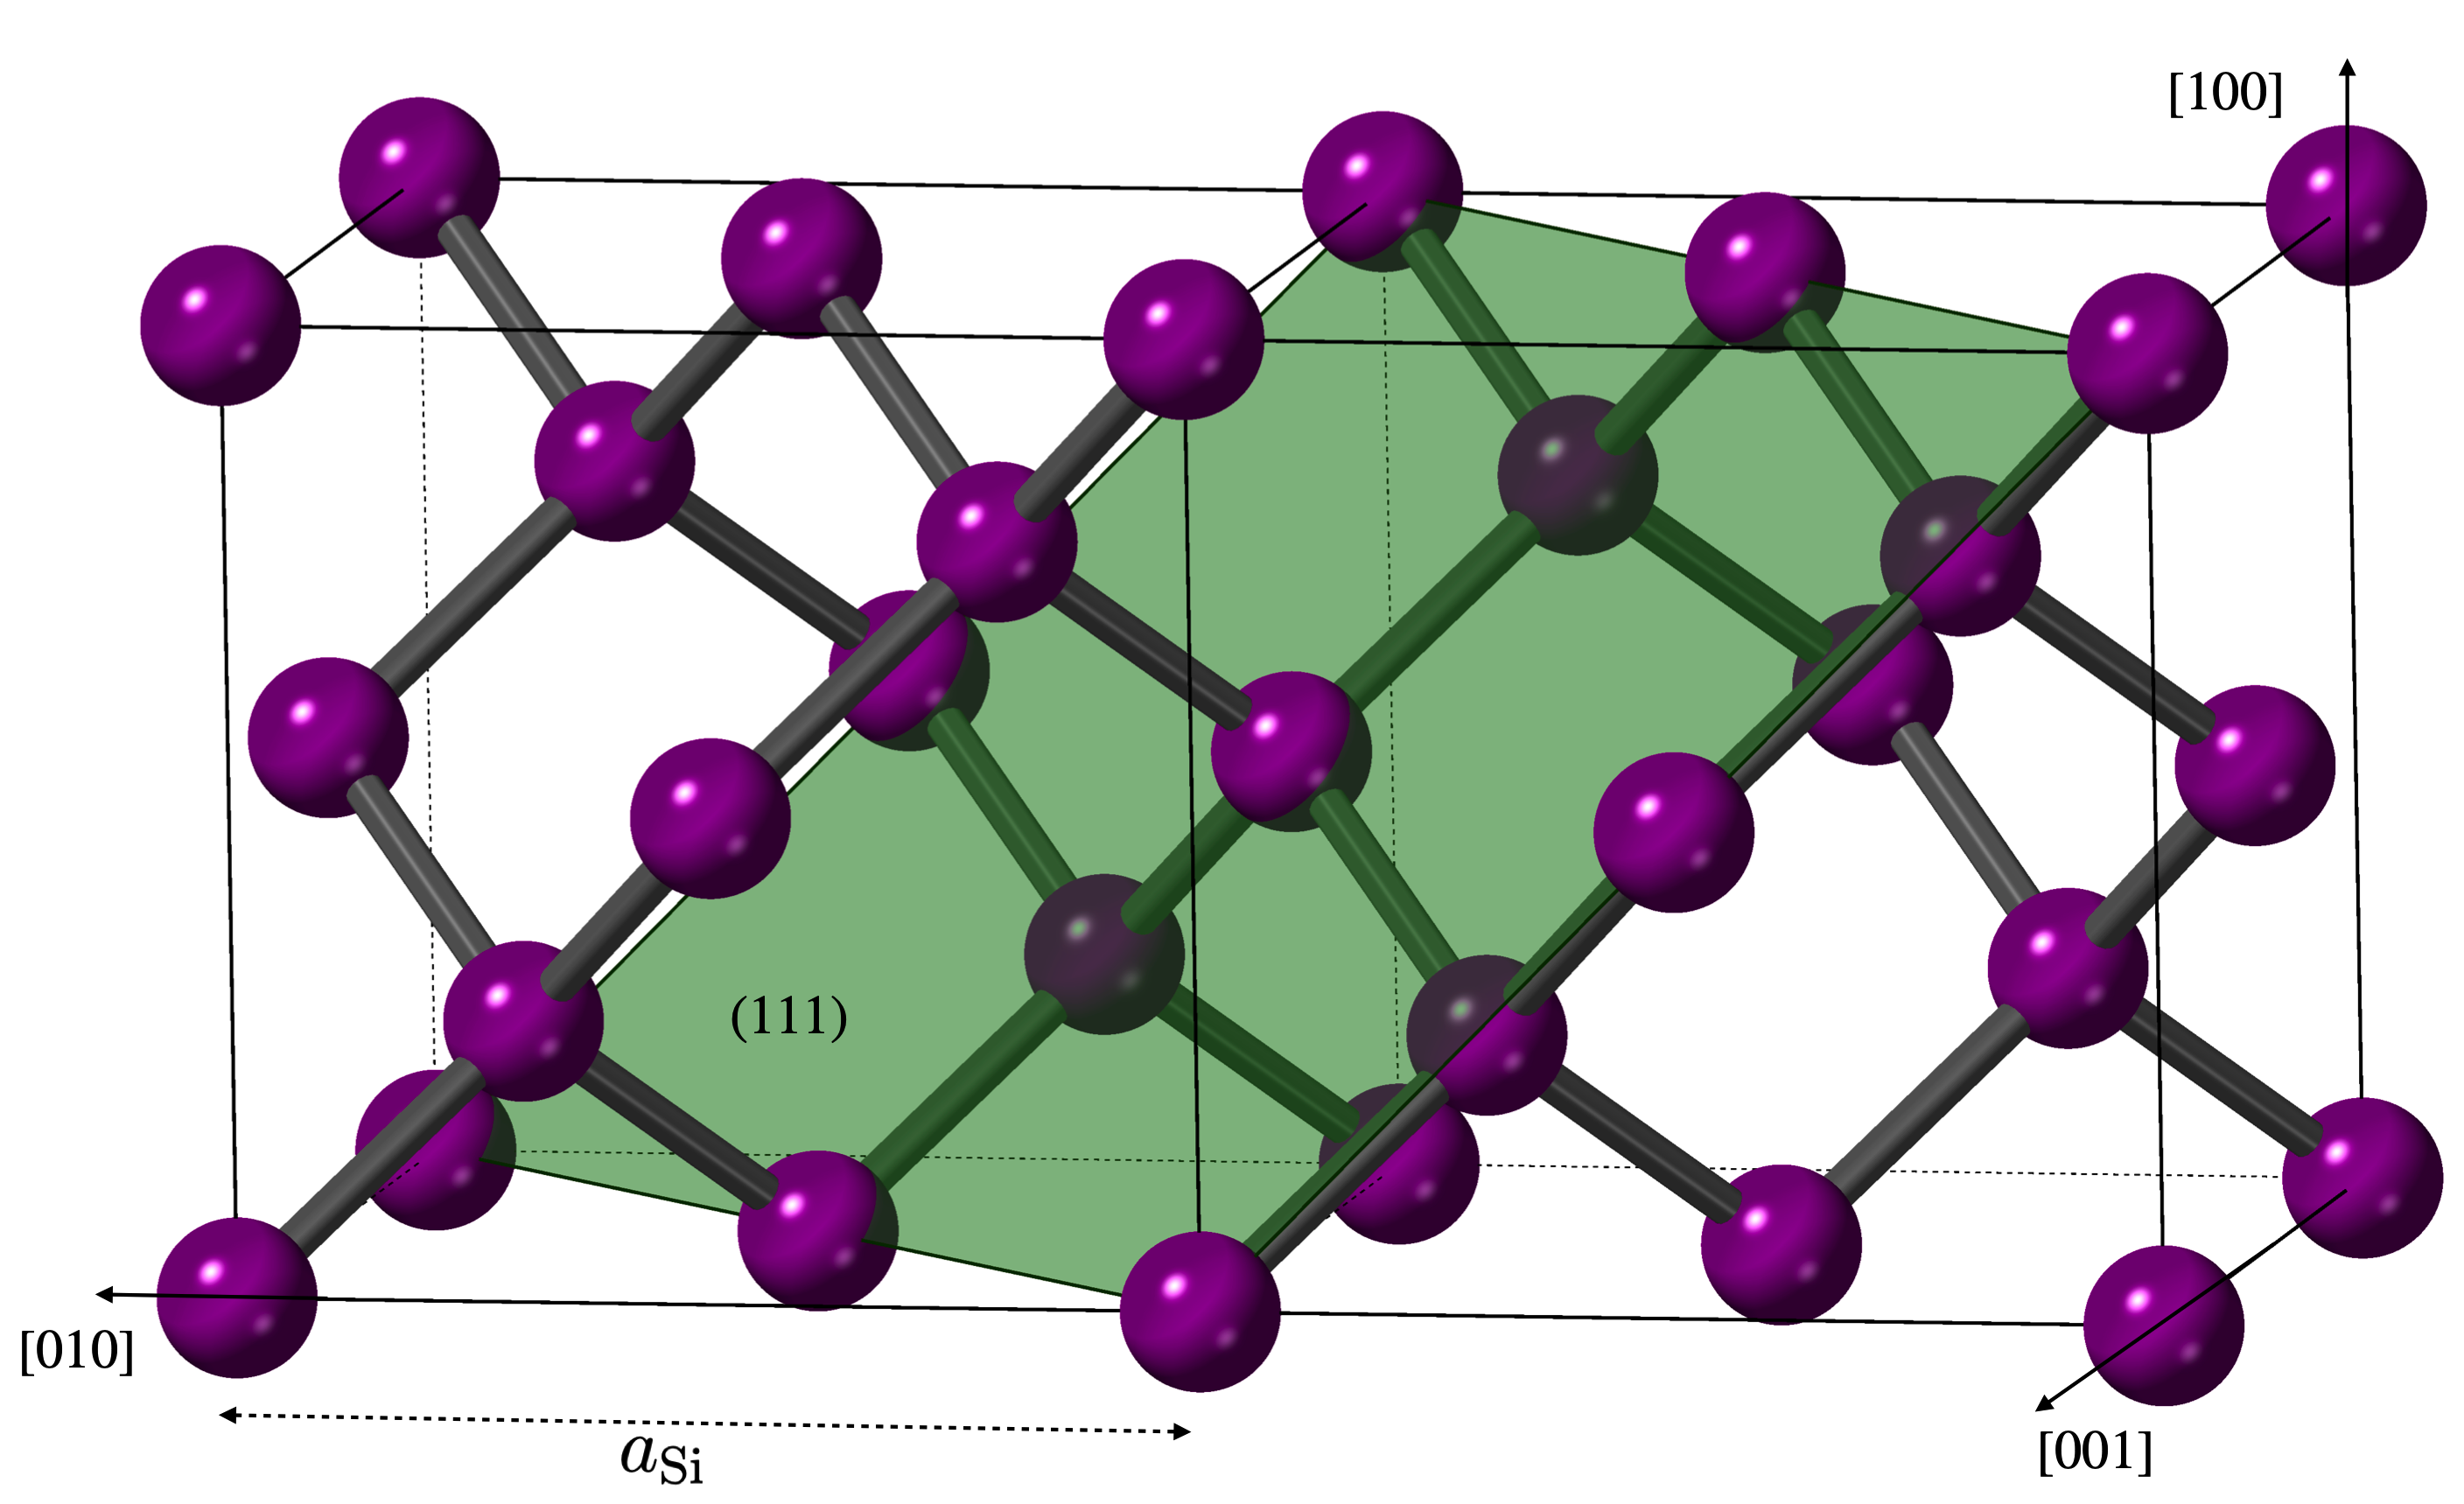
\includegraphics[scale=0.05]{Figures/crystal_fig2_edit.png}
 \end{figure}
 \begin{figure}
 \centering
 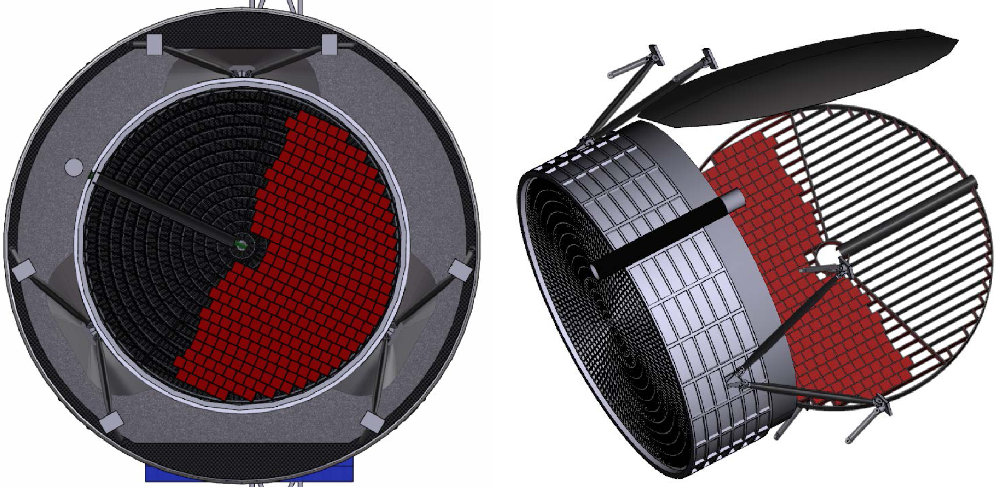
\includegraphics[scale=0.2]{Figures/JATIS_5_2_021002_f008_snip.png}
 \end{figure}
  \centering {\tiny Images:  T.\ Wood using \textsc{CrystalMaker} (\emph{top}), McEntaffter~2019 (\emph{bottom})}
 \end{minipage}
\hfill
\begin{minipage}[t]{0.6\linewidth}
\vspace{-5mm}
 \begin{block}{\textbf{Grating fabrication limitations}}
\begin{enumerate}
  \item {\large \underline{Dependence on silicon crystal structure}}
  \begin{itemize}%[label=(\alph*)]
      \item Cubic structure of silicon prevents formation of fanned grooves with smooth, continuous triangular facets
      %\item $\Delta d \equiv (a_{\text{Si}}/\sqrt{3}) \sin \left( \delta \right) \approx \SI{0.15}{\nm} \ \ \text{for} \ \ \delta = 29.5^{\circ}$
      \item[$\implies$] {\large Limits $\mathscr{R}$ and hence $\text{FOM}_{\text{weak}} \propto \sqrt{A_{\text{col}} \mathscr{R}}$}
    %\end{itemize}
    \end{itemize}
  %and additionally,  
  \item {\large \underline{Throughput of UV-NIL}}
  \begin{itemize}%[label=(\alph*)]
      \item Rigidity of thick silicon stamp requires applied pressure to achieve conformal contact %between stamp and resist-coated blank substrate for large-area imprints %(so that air pockets that give rise to unpatterned areas can be avoided)
      \item High pressure can lead to imperfections from particulate contaminants, trapped air pockets%damage to stamp surface
      \item Tens of quality imprints from single stamp 
      \item[$\implies$] {\large Impractical for \emph{XGS}, sounding rockets}
    \end{itemize}
\end{enumerate}
\end{block}
 \end{minipage}
\end{frame}


\section{Beamline Characterization of Diffraction Efficiency}


\begin{frame}{Beamline Characterization of Diffraction Efficiency}
\begin{minipage}[t]{0.48\linewidth}
\begin{figure}
 \centering
 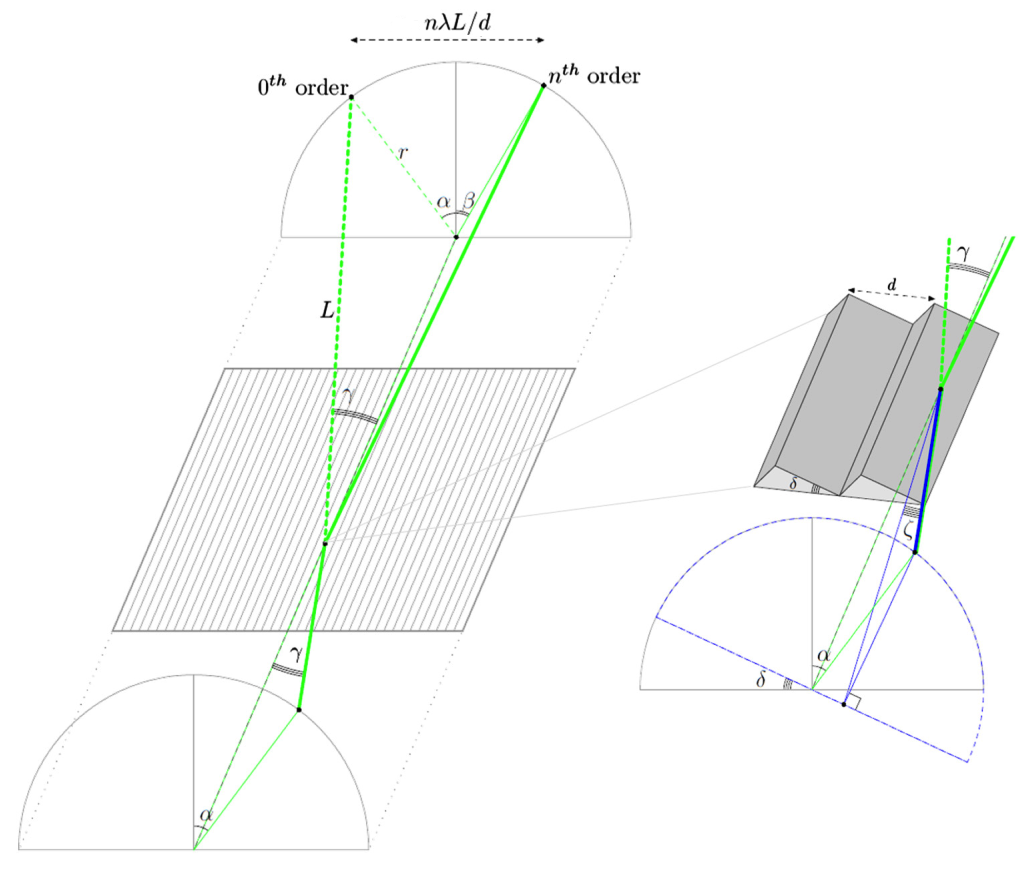
\includegraphics[scale=0.2]{Figures/grat_geo_fix.png}
 %\caption{Reflection grating geometry for conical diffraction}
 \end{figure}
 $\sin \left( \alpha \right) + \sin \left( \beta \right) = \frac{n \lambda}{d \sin \left( \gamma \right)} \quad \text{for } n = 0, \pm 1, \pm 2, \pm 3 ...$ 
 \end{minipage}
\hfill
\begin{minipage}[t]{0.48\linewidth}
 \textbf{X-ray grating considerations}
 \begin{enumerate}
 \item $\SI{250}{\electronvolt} \lessapprox \hbar \omega \lessapprox \SI{2}{\kilo\electronvolt}$ coincides with K-shell binding energies in low-to-mid $\mathcal{Z}$ atoms %spectrum of
 \begin{itemize}
  \item Soft x-rays easily absorbed by air
  \item High-$\mathcal{Z}$ materials beneficial for reflectivity
 \end{itemize}
 \item $\SI{5}{\nm} \gtrapprox \lambda \gtrapprox \SI{0.5}{\nm}$ approaches atomic scale %($a_0 \approx \SI{0.05}{\nm}$)
  \begin{itemize}
  \item Coherent scattering occurs small angles
  \item Critical angle for \emph{total external reflection}: $\zeta_c (\omega)$
 \end{itemize}
 \item Extreme off-plane geometry
  \begin{itemize}
  %\item Favorable for grating arrays
  %\item Facet graze angle must be small 
  \item $\sin \left( \zeta \right) = \sin \left( \gamma \right) \cos \left( \delta - \alpha \right)$ with $\zeta < \zeta_c (\omega)$
  \item Tune $d$ and $\delta$ to maximize diffraction efficiency near $\lambda_b$ with $\beta = 2 \delta - \alpha $
 \end{itemize}
\end{enumerate}
 %\vspace{-2mm}
  \begin{block}{\footnotesize \emph{Blaze wavelength}}
  \centering
  {$\lambda_b = \frac{d \sin \left( \gamma \right)}{n} \left[ \sin \left( \alpha \right) + \sin \left( 2 \delta - \alpha \right) \right]$ \newline \newline \text{\emph{Littrow configuration}}: $\alpha = \beta = \delta$ \text{ with } $\zeta = \gamma$}
  \end{block}
 \end{minipage}
\end{frame}

\begin{frame}{Beamline Characterization of Diffraction Efficiency}
\begin{minipage}[t]{0.48\linewidth}
\vspace{-4mm}
\begin{figure}
 \centering
 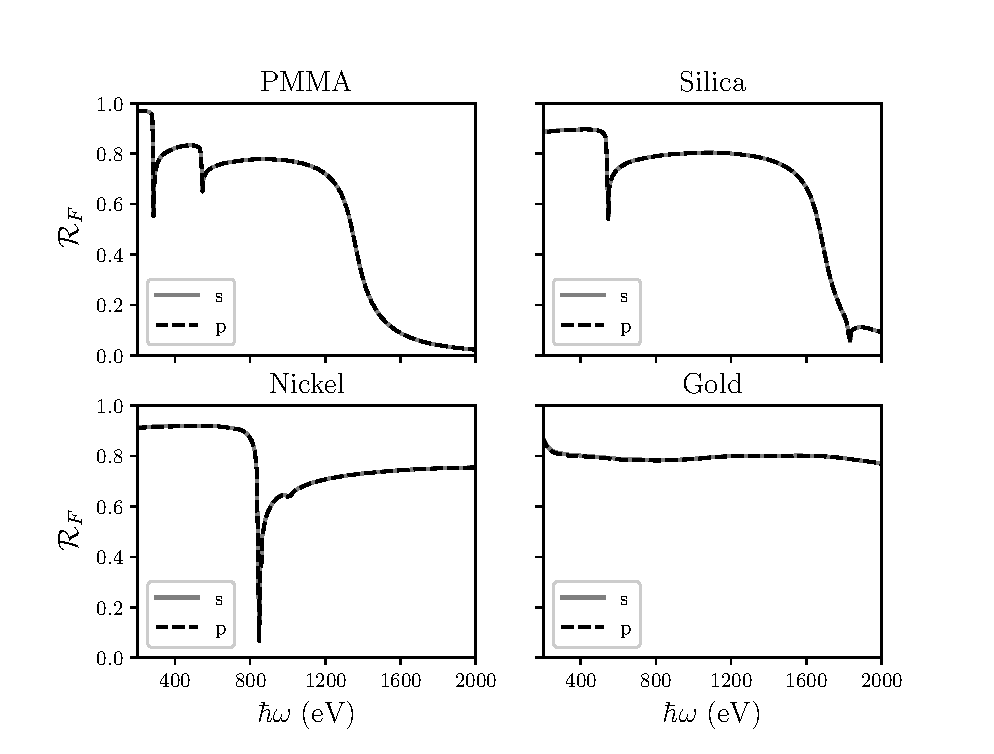
\includegraphics[scale=0.48]{Figures/X-ray_refl.eps}
 \vspace{-6mm}
 \caption{Fresnel soft x-ray reflectivity at $\zeta = 1^{\circ}$ (CXRO)}%{Fresnel soft x-ray reflectivity in orthogonal polarizations at $\zeta = 1^{\circ}$ for PMMA (\ce{C5H8O2})$_n$, silica (\ce{SiO2}), nickel (\ce{Ni}) and gold (\ce{Au}), demonstrating lack of polarization sensitivity (data obtained from CXRO \cite{CXRO_database})}\label{fig:X-ray_refl}
 \end{figure}
 \vspace{-4mm}
 \centering {$ \mathcal{R}_F \approx \norm{ \frac{\sin \left( \zeta \right) - \sqrt{\tilde{\nu}^2 (\omega) - \cos^2 \left( \zeta \right)}}{\sin \left( \zeta \right) + \sqrt{\tilde{\nu}^2 (\omega) - \cos^2 \left( \zeta \right)}} }^2$}
 %{\quad \quad \quad \quad \quad $ \mathcal{R}_F \approx \norm{ \frac{\sin \left( \zeta \right) - \sqrt{\tilde{\nu}^2 (\omega) - \cos^2 \left( \zeta \right)}}{\sin \left( \zeta \right) + \sqrt{\tilde{\nu}^2 (\omega) - \cos^2 \left( \zeta \right)}} }^2$}
 \end{minipage}
\hfill
\begin{minipage}[t]{0.48\linewidth}
\vspace{-4mm}
\begin{figure}
 \centering
 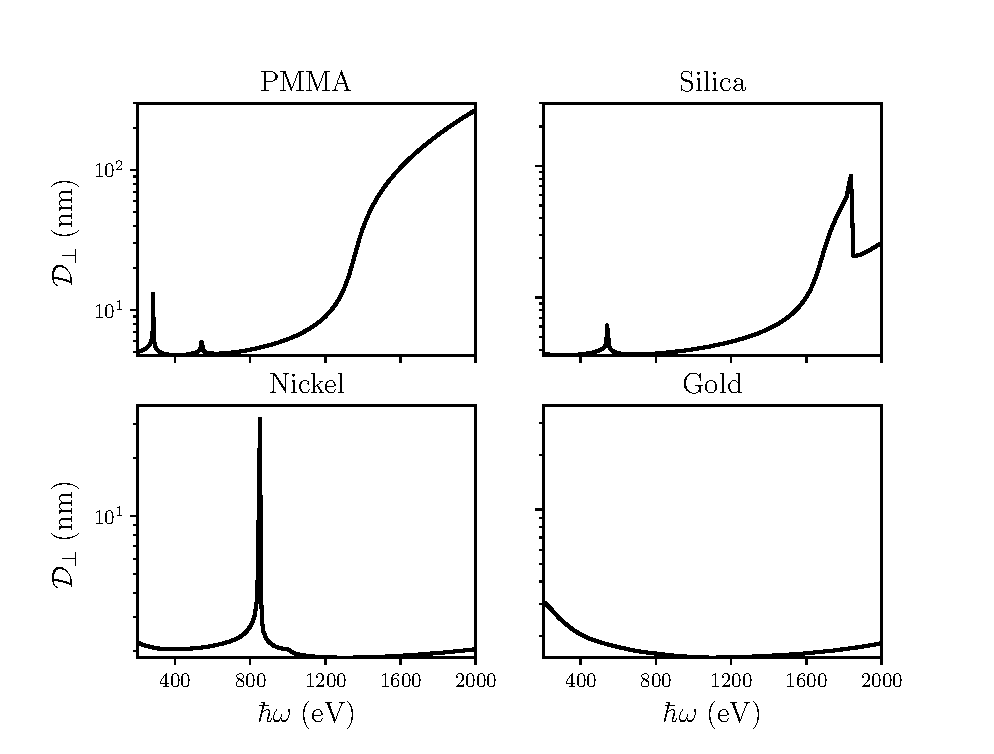
\includegraphics[scale=0.48]{Figures/X-ray_atten.eps}
 \vspace{-6mm}
 \caption{Total external reflection penetration depth at $\zeta = 1^{\circ}$}%{Total external reflection penetration depth, $\mathcal{D}_{\perp}$, at $\zeta = 1^{\circ}$ for PMMA, silica, nickel and gold (data obtained from CXRO \cite{CXRO_database})}\label{fig:X-ray_atten}
 \end{figure}
 \vspace{-4mm} 
 \centering {$\mathcal{D}_{\perp} = \frac{\lambda}{4 \pi \, \text{Im} \! \left[ \sqrt{\tilde{\nu}^2 (\omega) - \cos^2 \left( \zeta \right)} \right]}$}
 %{\quad \quad \quad \quad \quad $\mathcal{D}_{\perp} = \frac{\lambda}{4 \pi \, \text{Im} \! \left[ \sqrt{\tilde{\nu}^2 (\omega) - \cos^2 \left( \zeta \right)} \right]}$}
 \end{minipage}
\end{frame}

\subsection{Grating Testing at the Advanced Light Source (ALS)}

\begin{frame}{Beamline Characterization of Diffraction Efficiency}
\begin{minipage}[t]{0.48\linewidth}
\vspace{-3mm}
\begin{figure}
 \centering
 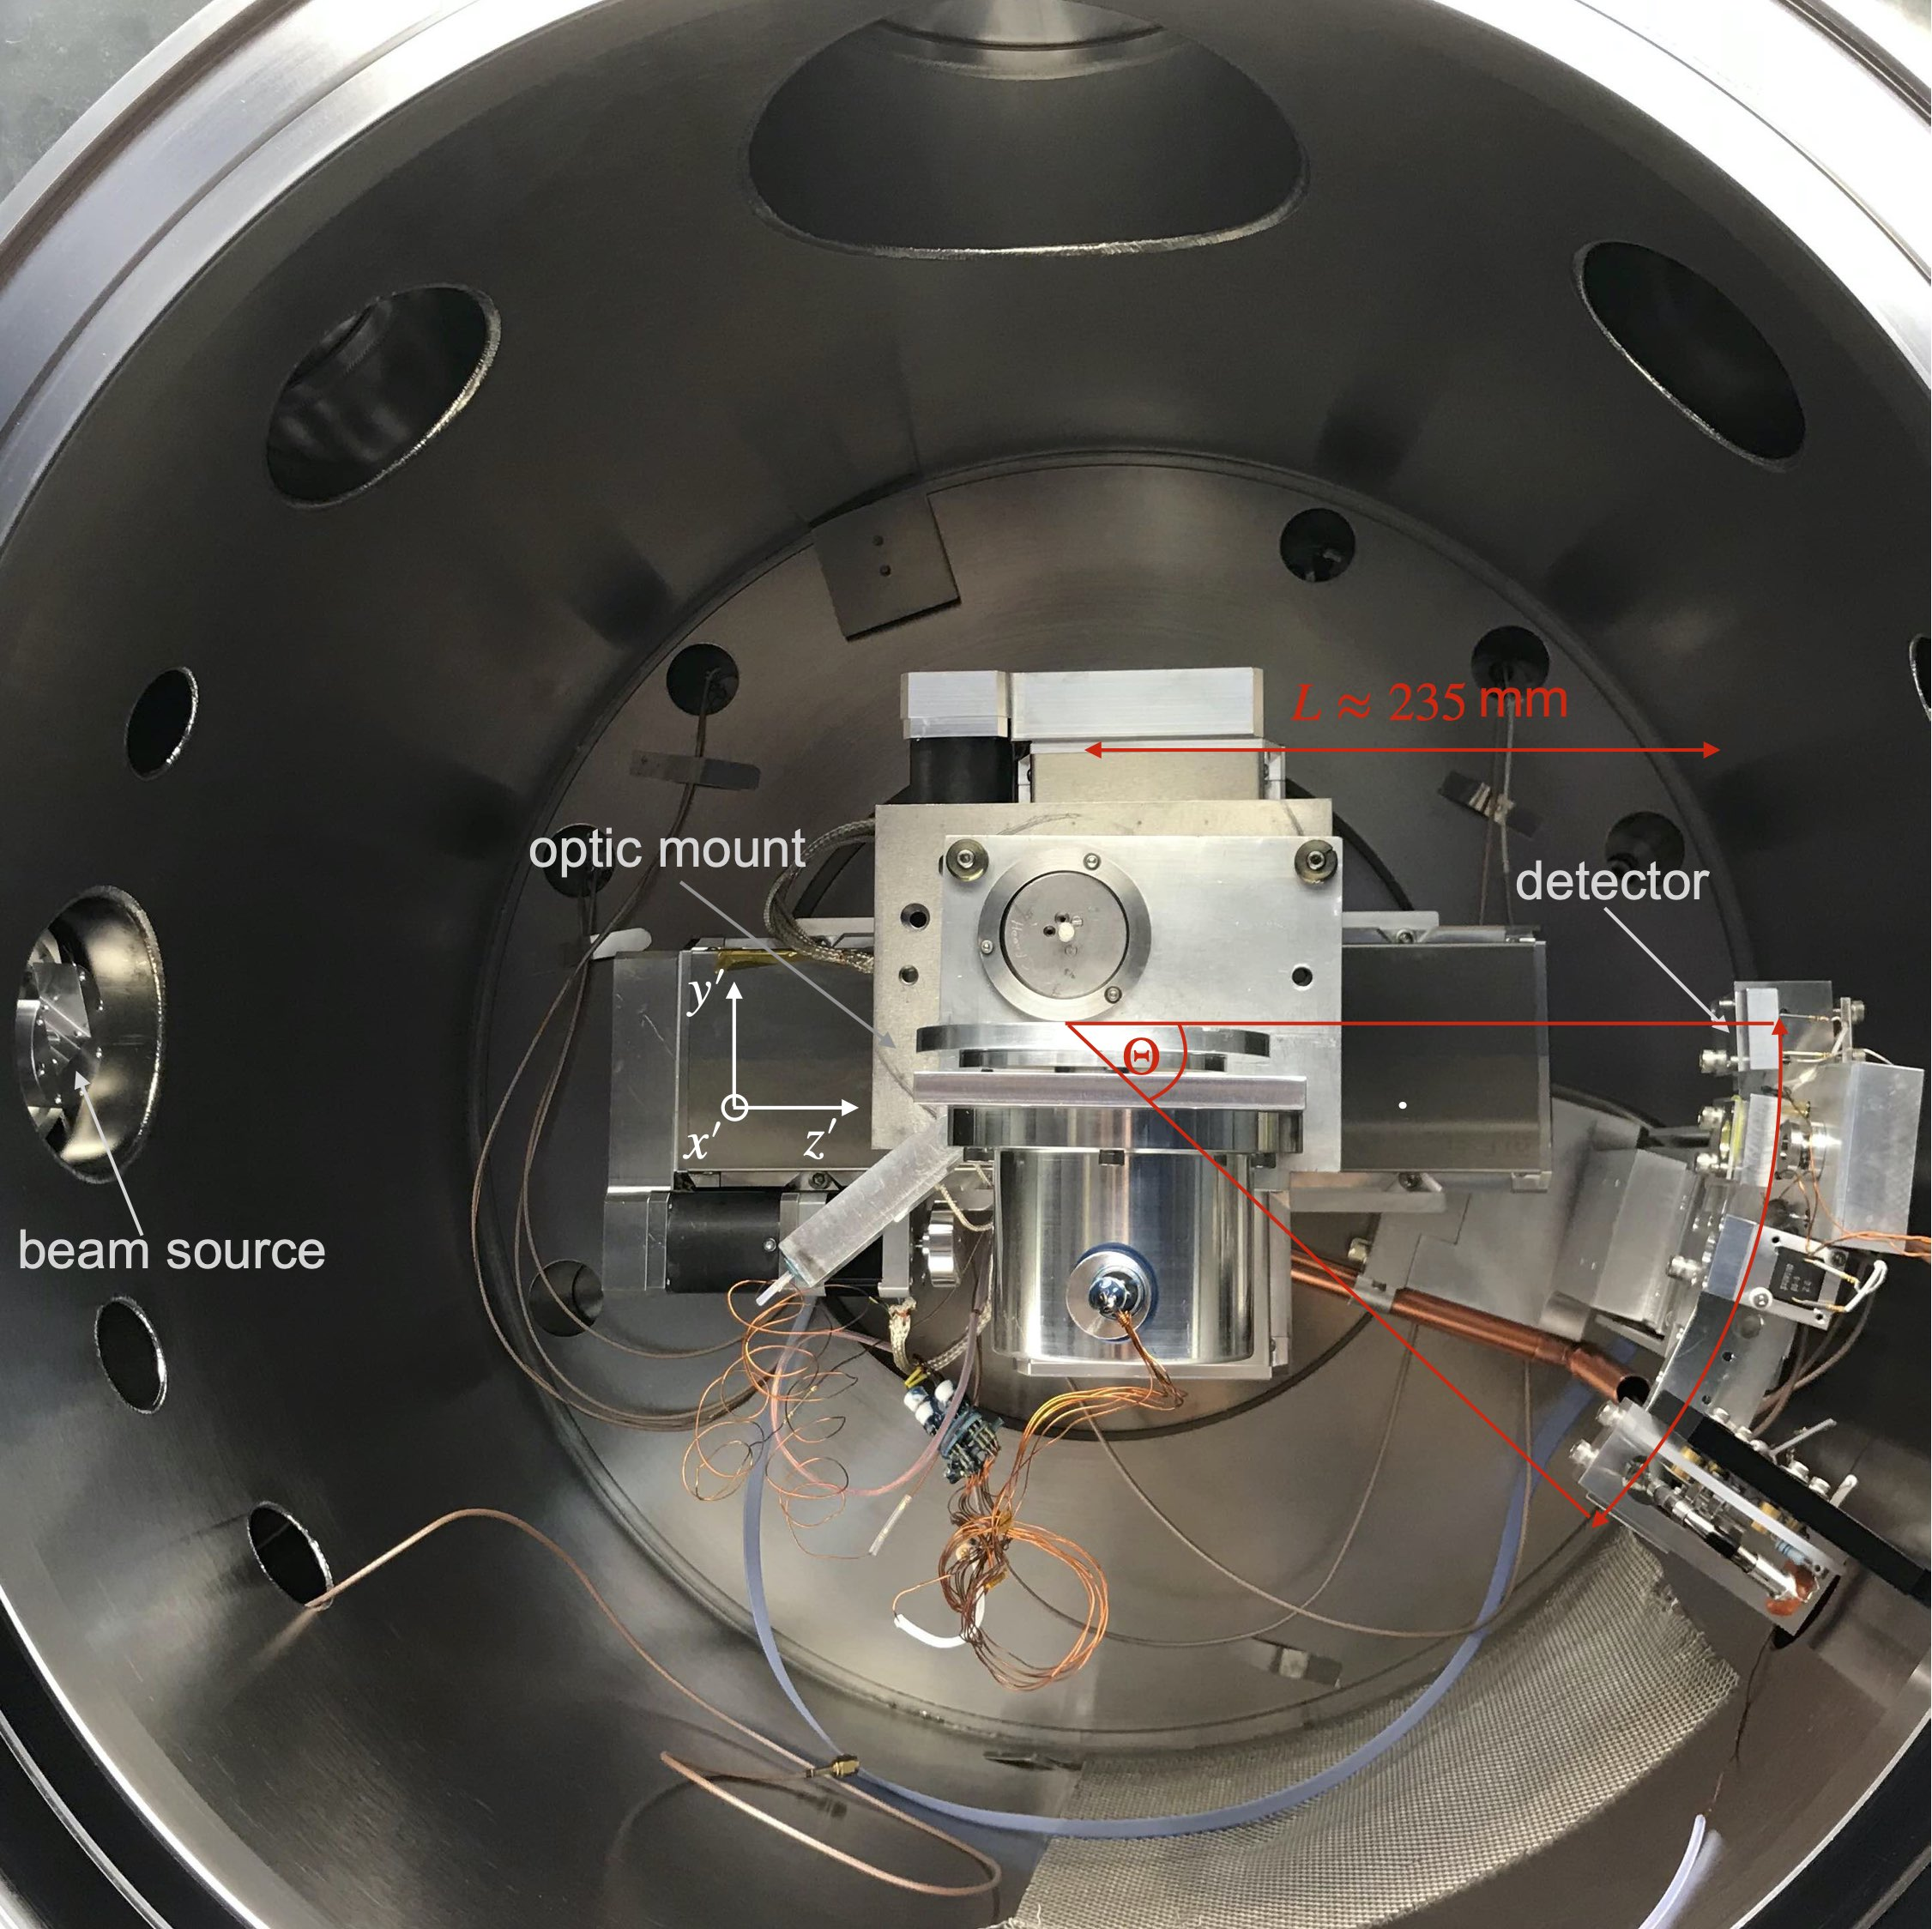
\includegraphics[scale=0.085]{Figures/ALS_photoA.jpg}
 \vspace{-2mm}
 \caption{Overview of beamline 6.3.2 of the ALS}%{Beamline 6.3.2 of the ALS provides a station for EUV and soft x-ray reflectometry, where a highly-coherent beam produced by a monochromator travels along the $z'$-direction to a photodiode attached to controllable staging that, due to the cylindrical shape of the vacuum chamber, can move linearly in the $x'$-direction and goniometrically in the $\Theta$-direction. A reflection grating is mounted on staging with translational and rotational degrees of freedom that can be moved to intercept the beam. This optic mount has rotational degrees of freedom that enable grating geometry to be set to a grazing-incidence, near-Littrow configuration.}\label{fig:beamline_photoA}
 \end{figure}
 \end{minipage}
\hfill
\begin{minipage}[t]{0.5\linewidth}
 \textbf{Advanced Light Source (ALS) beamline 6.3.2}
 \begin{itemize}
 \item Station for EUV and soft x-ray reflectometry
 \begin{itemize}
  \item[$\square$] Highly-coherent, monochromatic beam travels along the $z'$-direction to photodiode 
  \item[$\square$] Detector staging moves linearly in $x'$-direction, goniometrically in $\Theta$-direction
 \end{itemize}
 \item Use staging translational degrees of freedom (DOF) to position grating%intercept reflection grating with beam
 \item Use rotational DOF to set grating geometry in grazing-incidence, near-Littrow configuration
 \item Determine \emph{absolute diffraction efficiency}, $\mathscr{E}_n$, by measuring intensity of each propagating order, $\mathcal{I}_n$, to unobstructed beam, $\mathcal{I}_{\text{inc}}$ 
\end{itemize}
\begin{block}{\footnotesize \emph{Absolute diffraction efficiency}}
\centering {$\mathscr{E}_n  \equiv \frac{\mathcal{I}_n}{\mathcal{I}_{\text{inc}}} \quad \text{for } n = 0, \pm 1, \pm 2, \pm 3 ...$}
\end{block}
 \end{minipage}
\end{frame}

\begin{frame}{Beamline Characterization of Diffraction Efficiency}
\begin{minipage}[t]{0.3\linewidth}
\begin{figure}
 \centering
 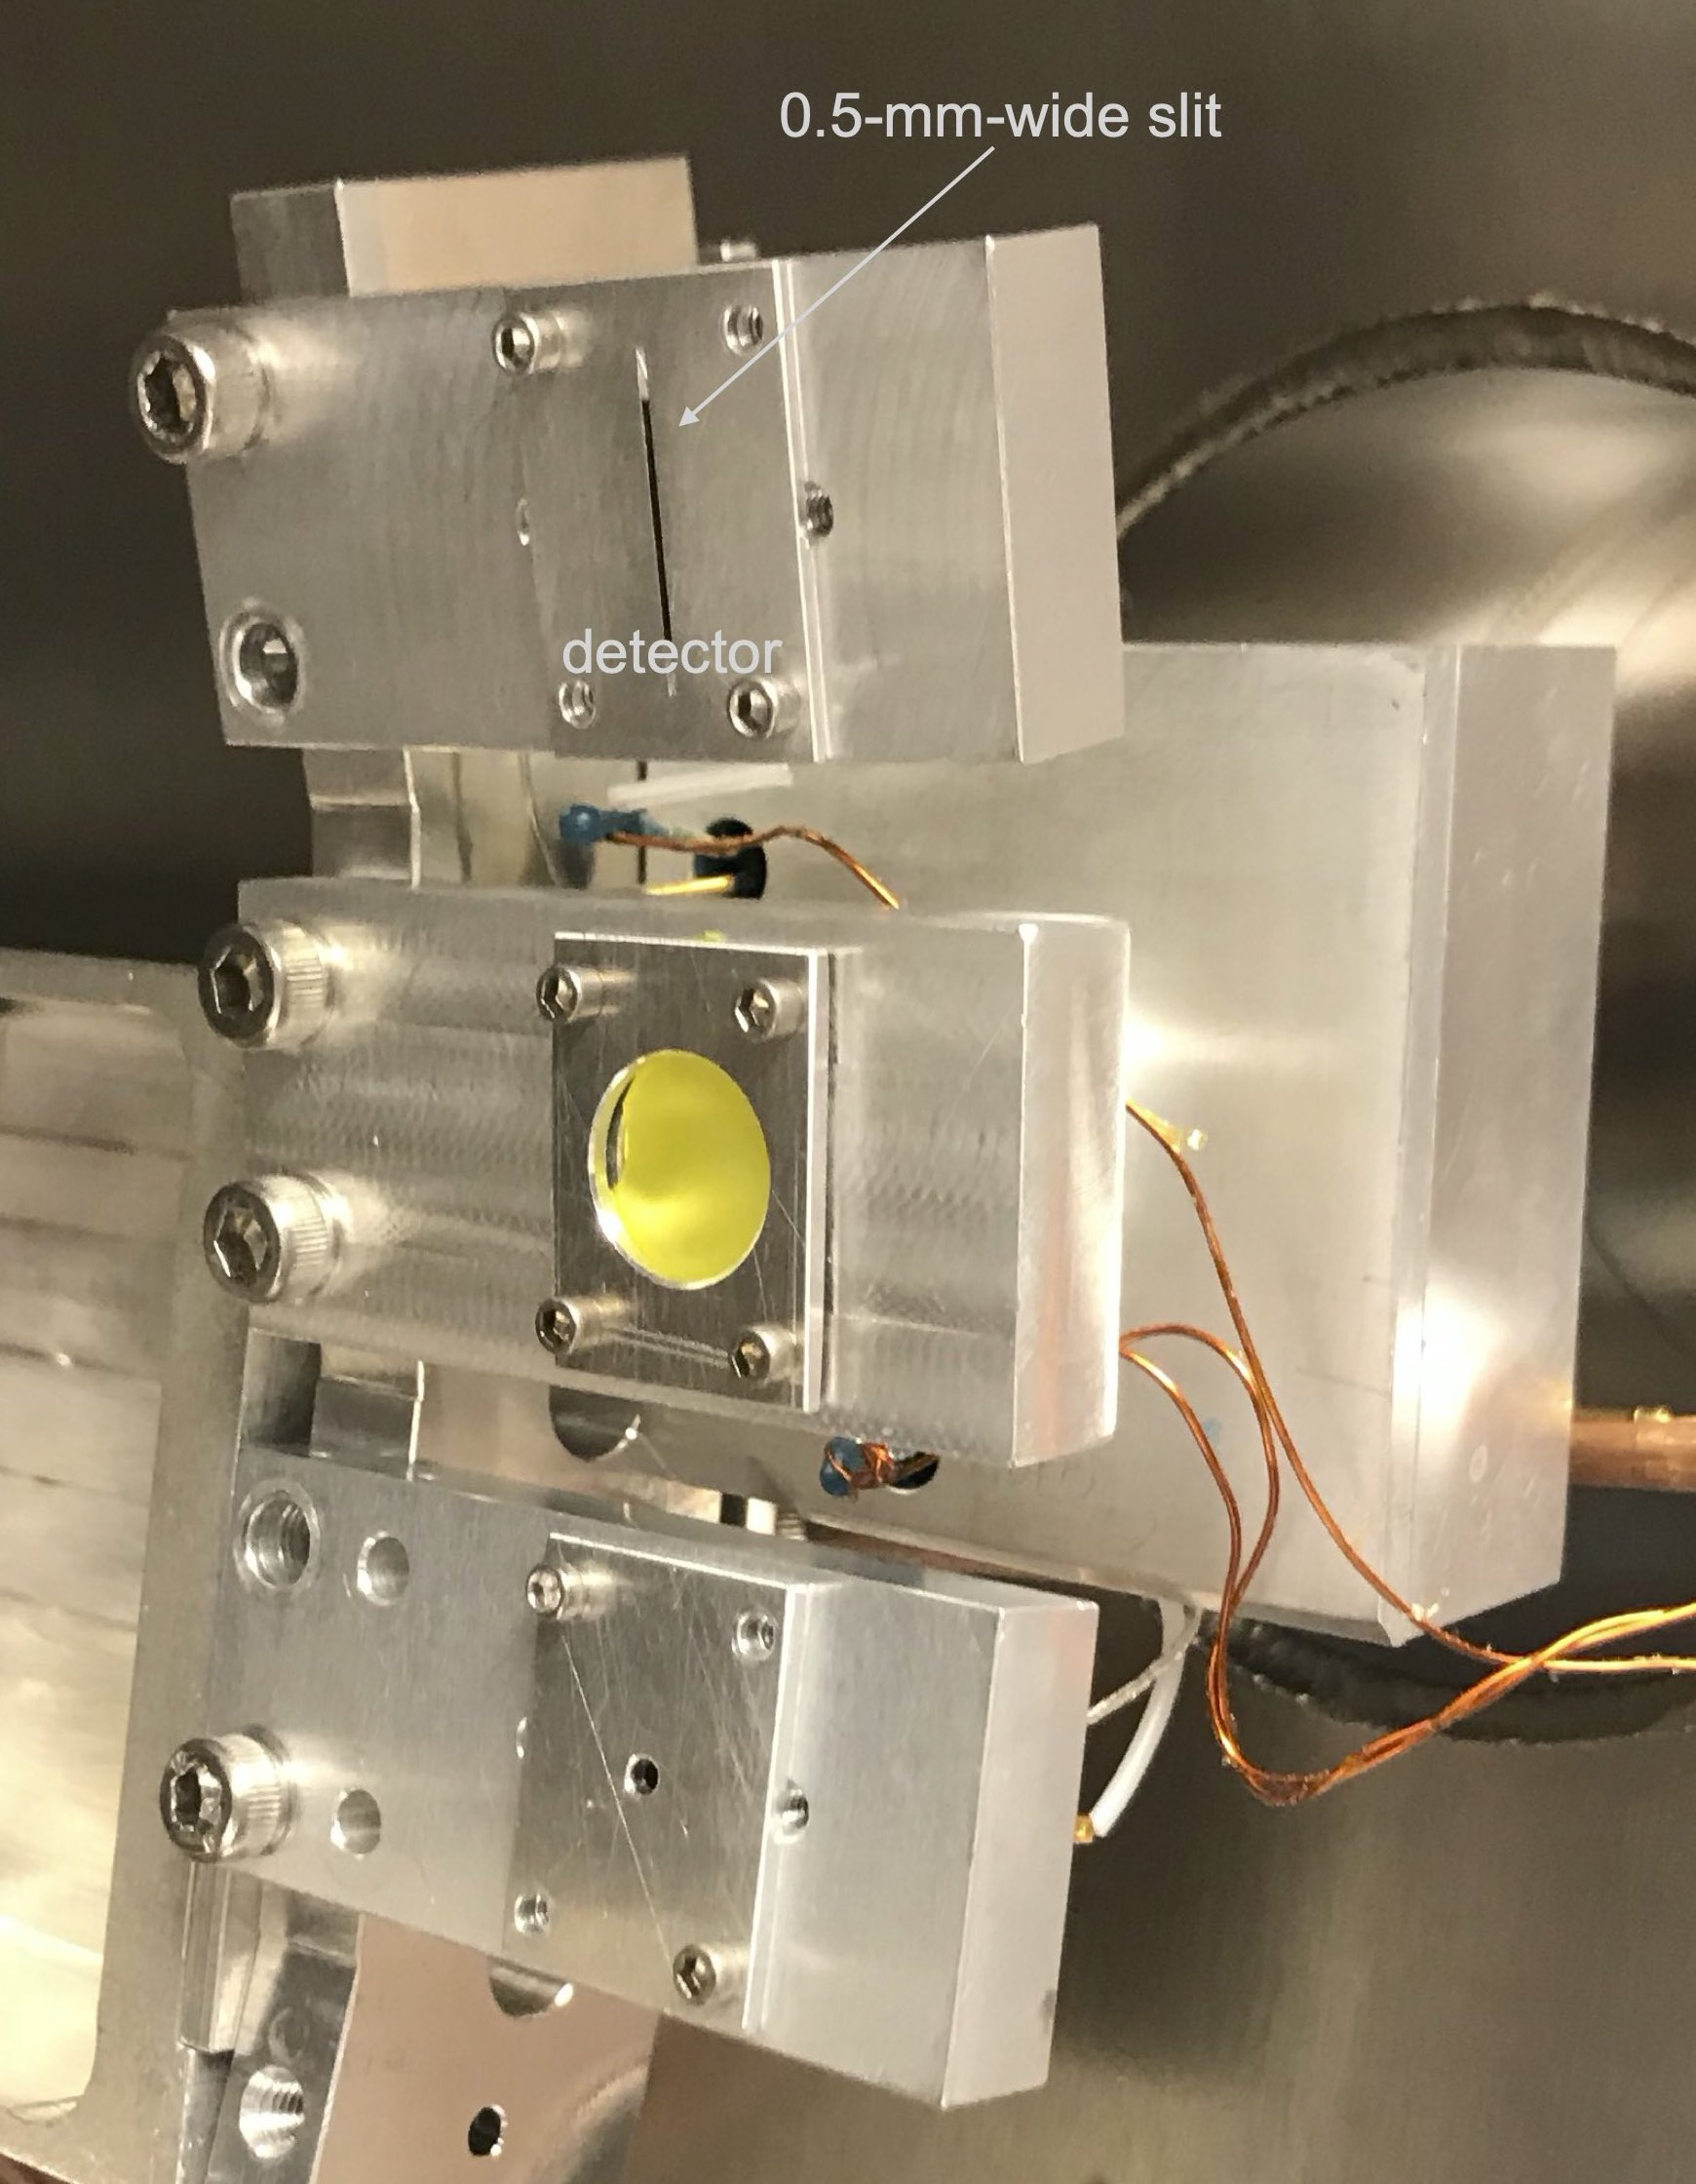
\includegraphics[scale=0.07]{Figures/ALS_photoC.jpg}
 \caption{View of masked photodiode detector on goniometric staging}%{Inside the test chamber shown in \cref{fig:beamline_photoA}, a \SI{0.5}{\mm}-wide, vertical slit is installed to mask the photodiode detector so as to allow the intensity of each propagating order, $\mathcal{I}_n \! \left( \lambda \right)$, to be measured in isolation. With the grating groove direction approximately aligned with the $z'$-axis for an extreme off-plane mount, the grating dispersion and cross-dispersion directions are approximately aligned with the linear $x'$-direction and the goniometric $y'$-direction motion of the detector staging, respectively.}\label{fig:beamline_photoB}
 \end{figure}
 \end{minipage}
 \hfill
\begin{minipage}[t]{0.69\linewidth}
\vspace{-3mm}
 \begin{figure}
 \centering
 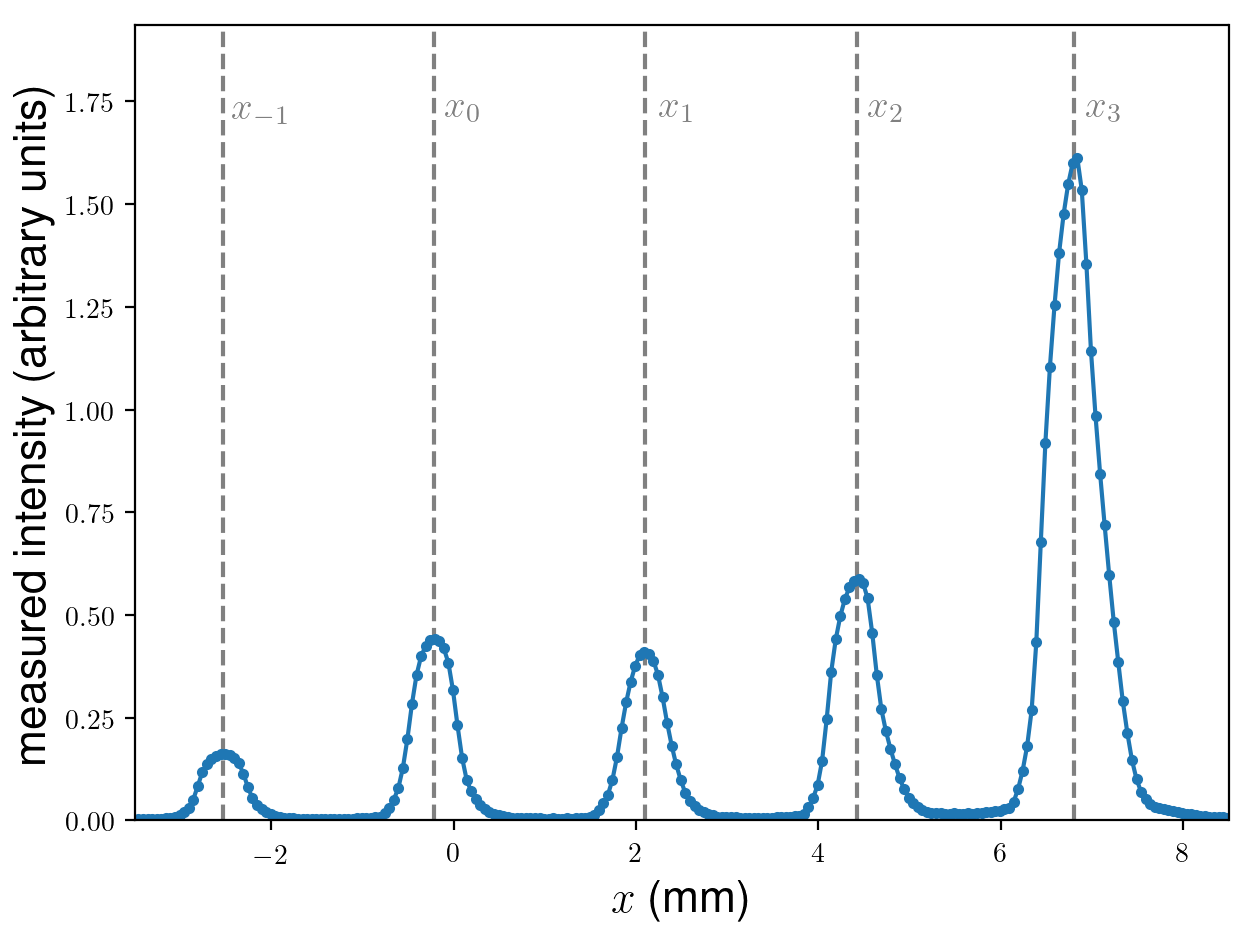
\includegraphics[scale=0.34]{Figures/ALS_xdata.png}
 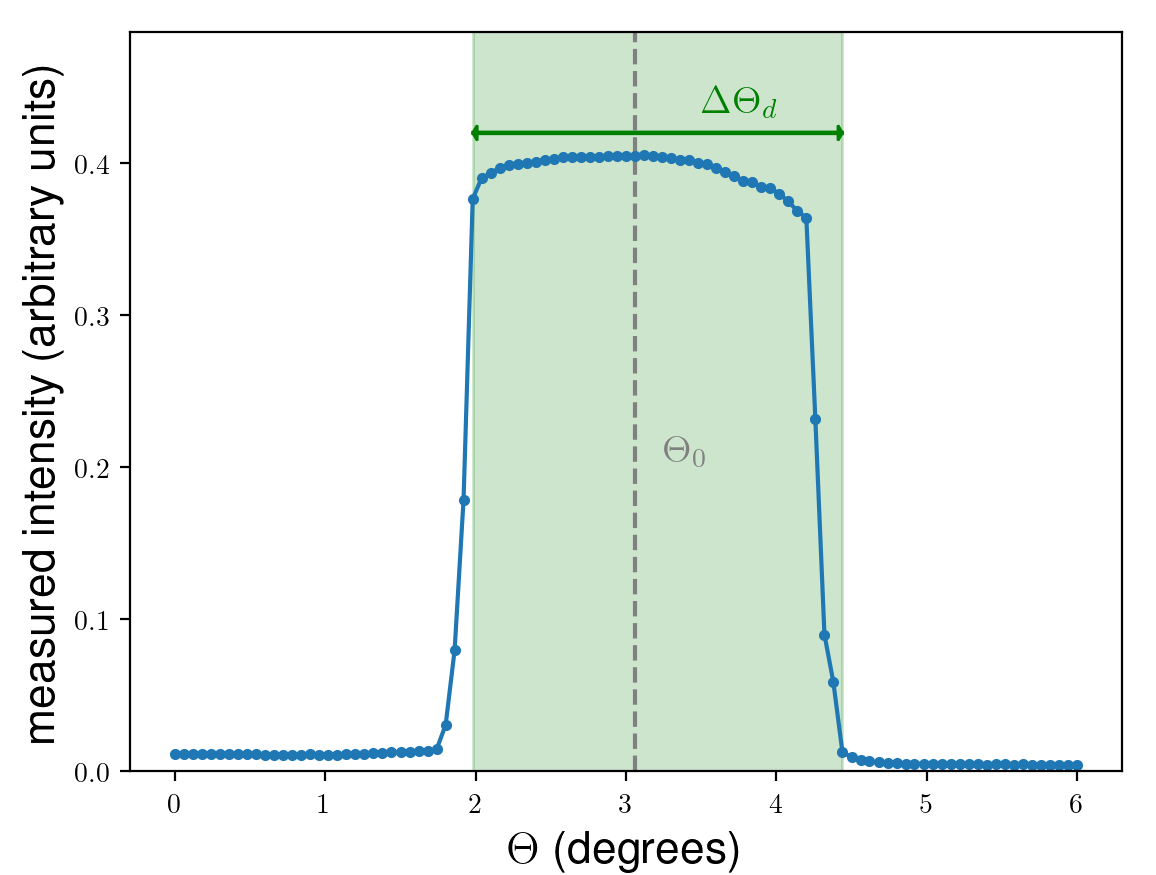
\includegraphics[scale=0.34]{Figures/ALS_ydata_cent_range.png}
 \vspace{-2mm}
 \caption{Example of measured intensity data for diffracted arc}%{Example of measured intensity data for the diffracted arc as a function of horizontal detector position, $x'$, in steps of \SI{50}{\um}. The $x$-component of each propagating order, $x_n$, is determined using the weighted-mean centroid of each local maximum spaced approximately by $n \lambda L /d$.}\label{fig:ALS_xdata}
 \end{figure}
 \vspace{-2mm}
 \begin{enumerate}
  \item Equip detector with \SI{0.5}{\mm}-wide, vertical slit $\implies$ order separation
  \begin{itemize}
    \item[$\square$] $\Delta x_n = n \lambda L / d$ $\sim$ millimeters with $L \approx \ell_{\text{det}} / \Delta \Theta_d \approx \SI{235}{\mm}$ 
  \end{itemize}
  \item Gather $(x_n,y_n)$ coordinates of propagating orders $\implies$ diffracted arc 
  \begin{itemize}
    \item[$\square$] $y_n = L \sin (\Theta_n)$ using goniometric staging
  \end{itemize}
  \item Determine $\gamma$ and $\alpha$ from arc radius, relative position of direct beam
  \begin{itemize}
    \item[$\square$] Adjust principal-axis angles for desired geometry
  \end{itemize}
 \end{enumerate}
 %\begin{figure}
 %\centering
 %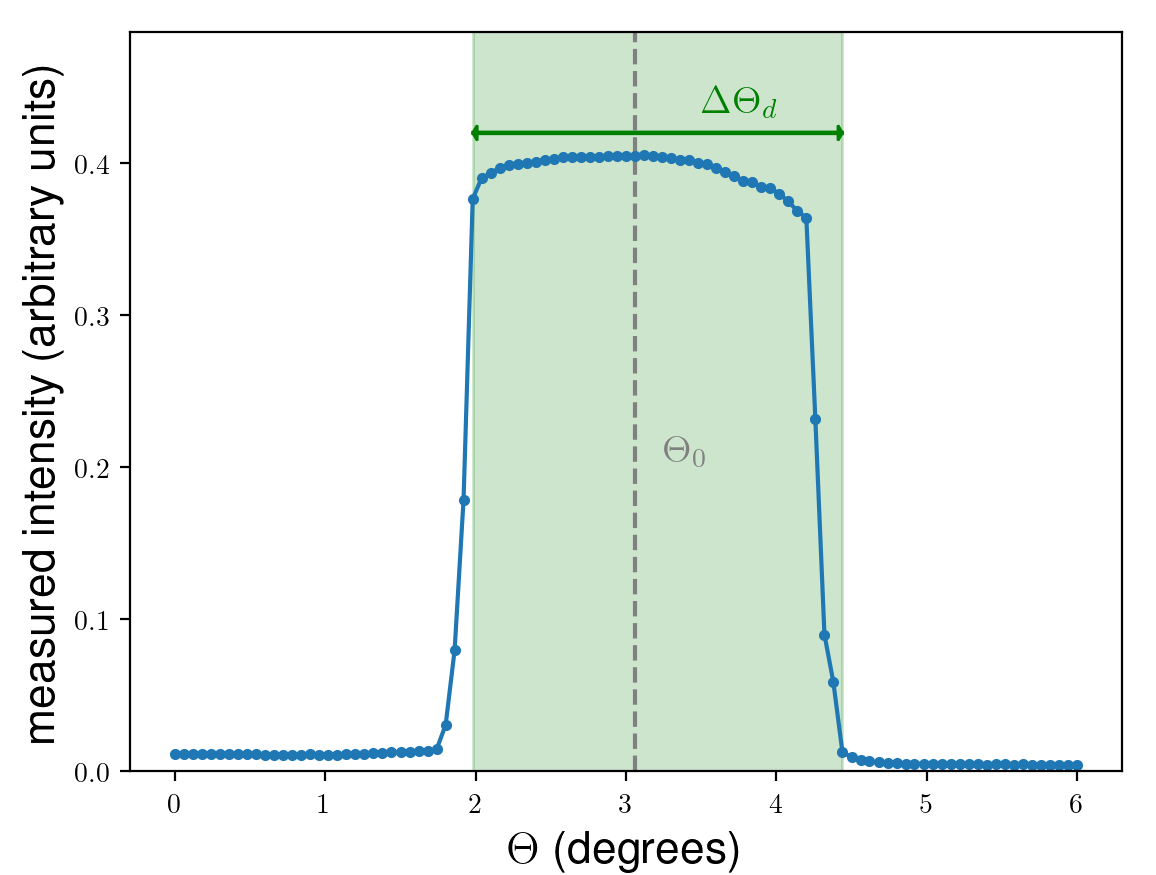
\includegraphics[scale=0.3]{Figures/ALS_ydata_cent_range.png}
 %\caption{Example of measured intensity data for a $0^{\text{th}}$-order diffracted beam as a function of goniometric angle}%{Example of measured intensity data for a $0^{\text{th}}$-order diffracted beam as a function of goniometric angle, $\Theta$, in steps of $\sim$0.06$^{\circ}$. The green shaded region highlights the measured angular size of the detector, $\Delta \Theta_d$, which corresponds to one full translation of the beam in the goniometric direction, along the long direction of the \SI{0.5}{\mm}-wide slit. Additionally, the goniometric centroid angle associated with the measured beam, $\Theta_0$, can be determined through a weighted mean calculation of the data. This process is repeated for each propagating order to derive $\Theta_n$ for the $n^{\text{th}}$ order and ultimately, the corresponding $y$-component, $y_n = L \sin \left( \Theta_n \right)$.}\label{fig:ALS_cent_throw}
 %\end{figure}
 \end{minipage}
\end{frame}

\subsection{Theoretical Modeling using \textsc{PCGrate-SX}}

\begin{frame}{Beamline Characterization of Diffraction Efficiency}
\vspace{-2mm}
\textbf{Modeling diffraction efficiency} %with \textsc{PCGrate-SX} (\textsc{I.\ I.\ G., Inc.\@})
 \begin{itemize}
  \item \textsc{PCGrate-SX} solves Helmholtz equation via \emph{integral method} for custom grating boundary, $\gamma$ and $\alpha$ %input by user
  \item Take into account reflectivity of groove facet
  \item Efficiency response for x-ray reflection gratings polarization insensitive (Marlowe, et al.~2016)
  %\item Marlowe, et al.~(2016) verified lack of polarization sensitivity for off-plane x-ray reflection gratings, modeling scheme using \emph{perfect conductivity mode} %assuming a perfectly conducting grating boundary with perfectly smooth groove facets and an incident wavefront with TE polarization
  %\item Assume \emph{perfect conductivity}, modulate predicted diffraction efficiency by $\mathcal{R}_F$ of user-input, stratified medium defined by $\tilde{\nu}(\omega)$ data, custom layers
 \end{itemize}
\vspace{-1mm}
\begin{figure}
 \centering
 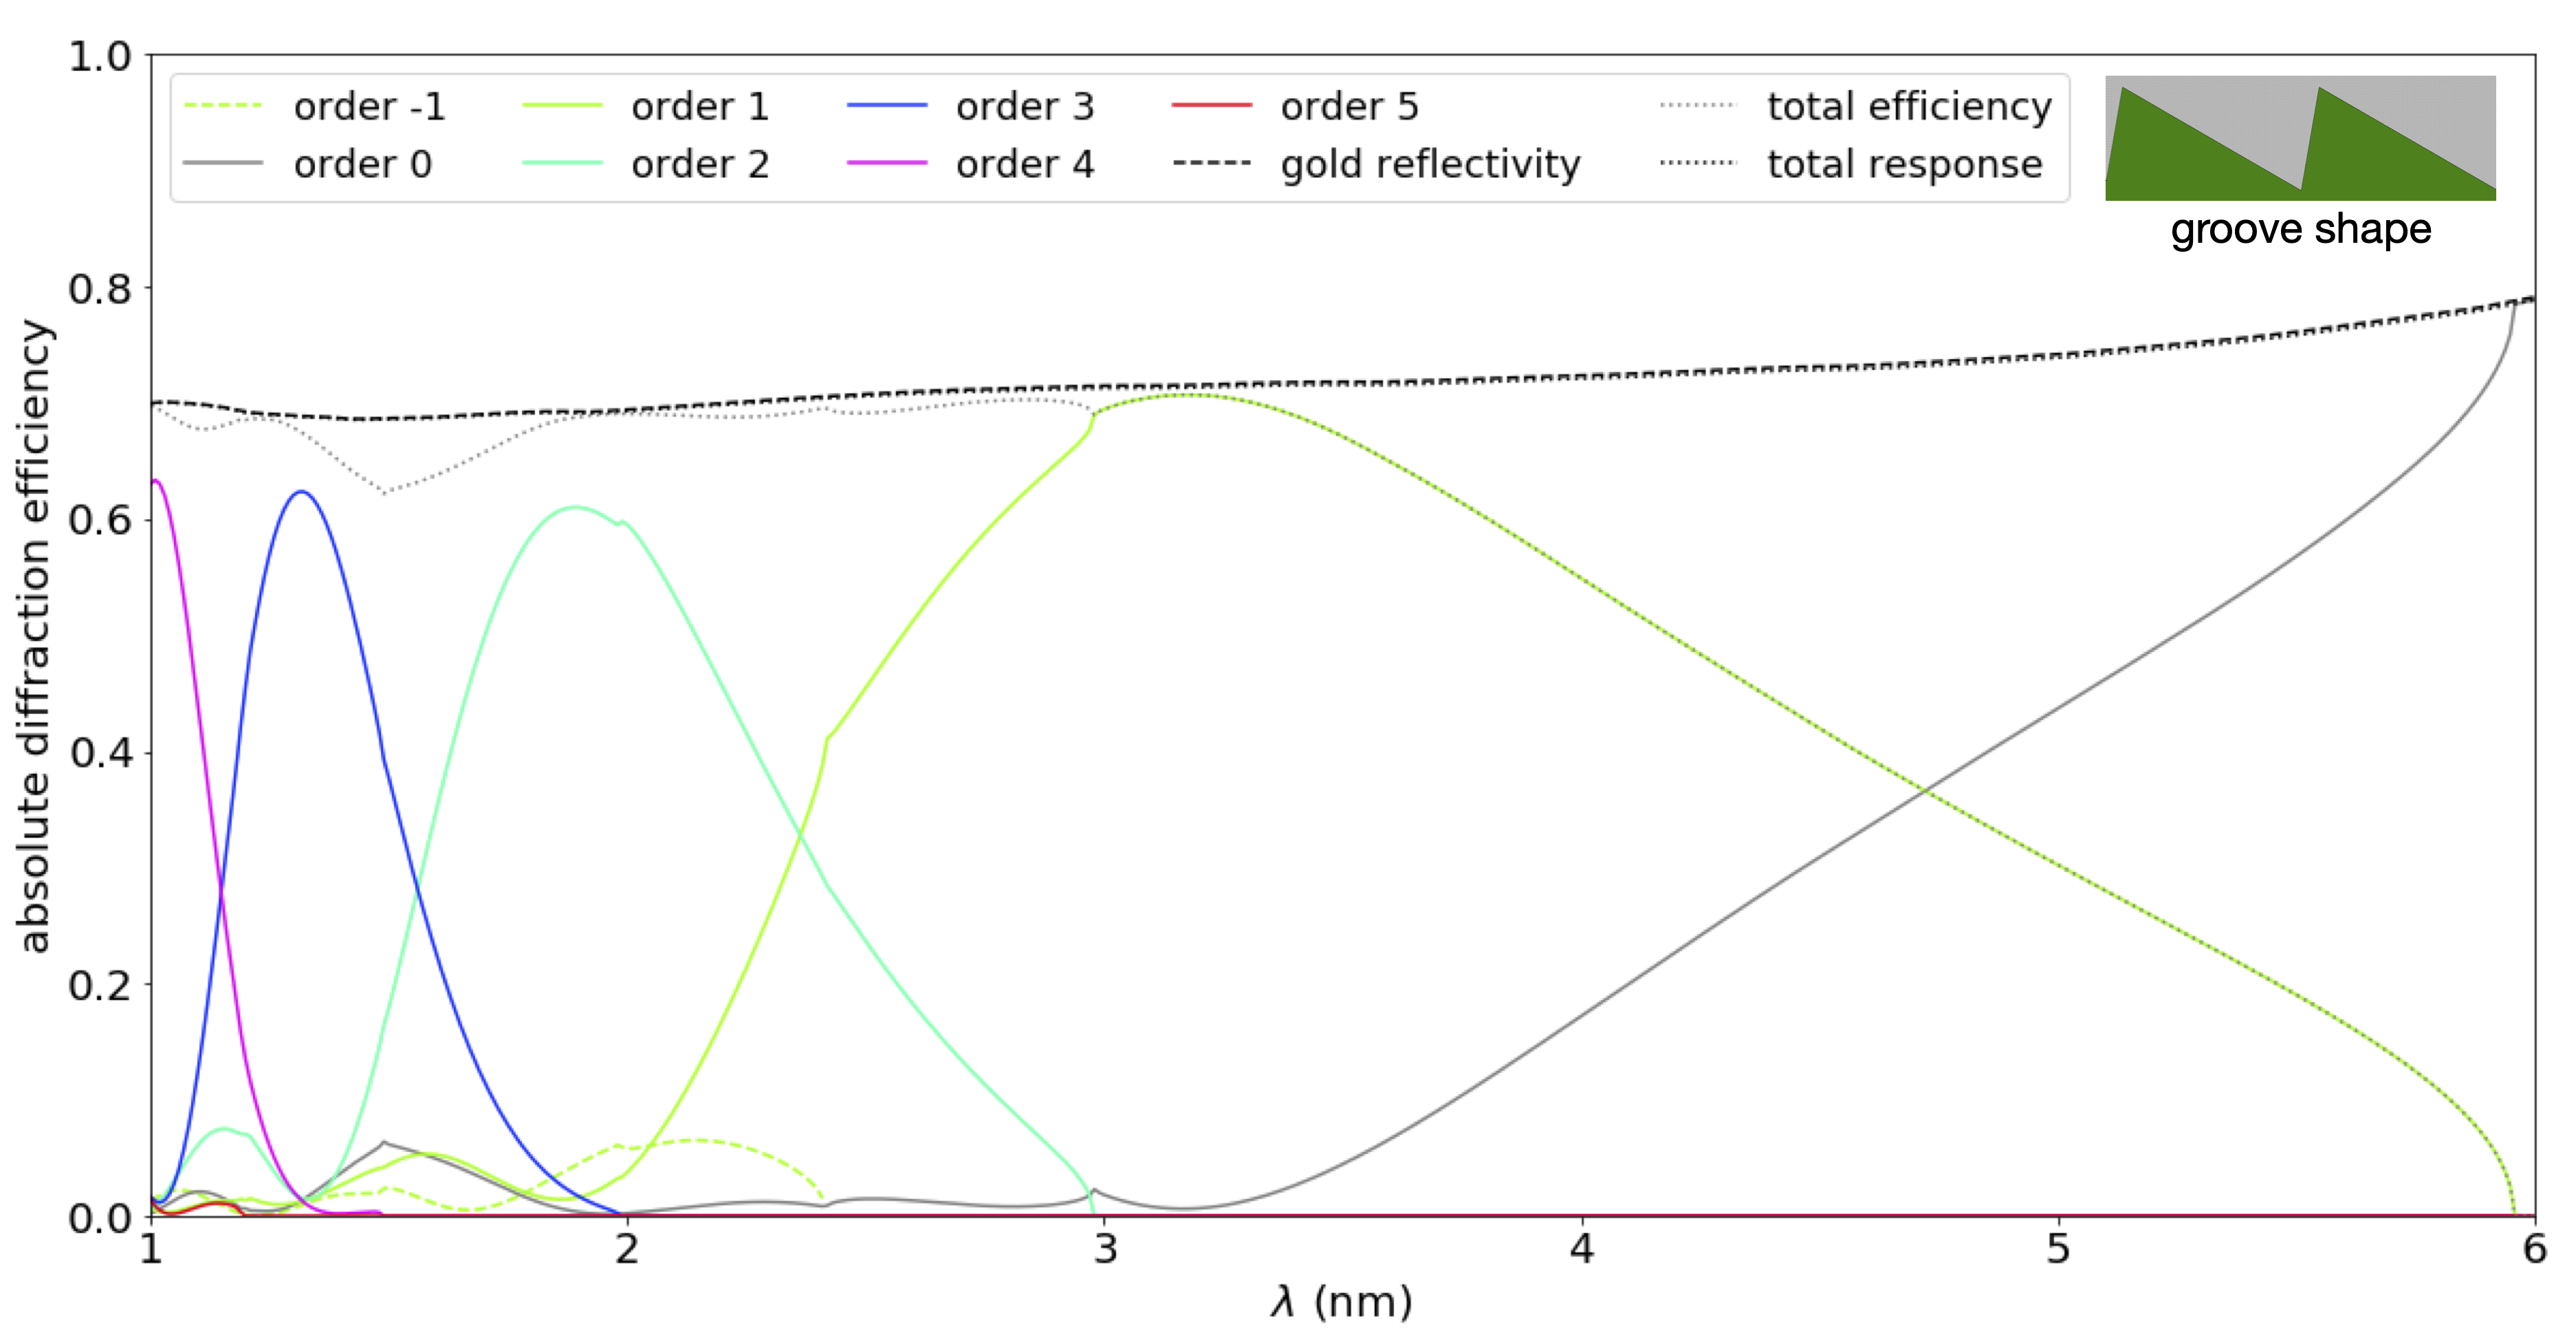
\includegraphics[scale=0.17]{Figures/au_ex.png}
 %\vspace{-2mm}
 %\caption{Example of predicted diffraction efficiency for a gold grating using \textsc{PCGrate-SX} under perfect conductivity mode}%{Example of predicted diffraction efficiency for a gold grating using \textsc{PCGrate-SX} (v.\ 6.1) under perfect conductivity mode using the same parameters as \cref{fig:pcgrate_example_perf}. The total response of the grating predicted by \textsc{PCGrate-SX} very closely matches Fresnel reflectivity of an equivalent surface at a grazing incidence angle $\zeta \equiv \arcsin \left[ \sin \left( \gamma \right) \cos \left( \delta - \alpha \right) \right]$.}\label{fig:pcgrate_example_au}
 \end{figure}
\end{frame}

%\begin{frame}{Beamline Characterization of Diffraction Efficiency}
%\begin{minipage}[t]{0.54\linewidth}
%\textbf{Modeling diffraction efficiency} %with \textsc{PCGrate-SX} (\textsc{I.\ I.\ G., Inc.\@})
% \begin{itemize}
%  \item \textsc{PCGrate-SX} solves Helmholtz equation via \emph{integral method} for custom grating boundary, $\gamma$ and $\alpha$ %input by user
%  \item Marlowe, et al.~2016 verified lack of polarization sensitivity for off-plane x-ray reflection gratings, modeling scheme using \emph{perfect conductivity mode} %assuming a perfectly conducting grating boundary with perfectly smooth groove facets and an incident wavefront with TE polarization
  %\item Assume \emph{perfect conductivity}, modulate predicted diffraction efficiency by $\mathcal{R}_F$ of user-input, stratified medium defined by $\tilde{\nu}(\omega)$ data, custom layers
% \end{itemize}
%\vspace{-2mm}
%\begin{figure}
% \centering
% 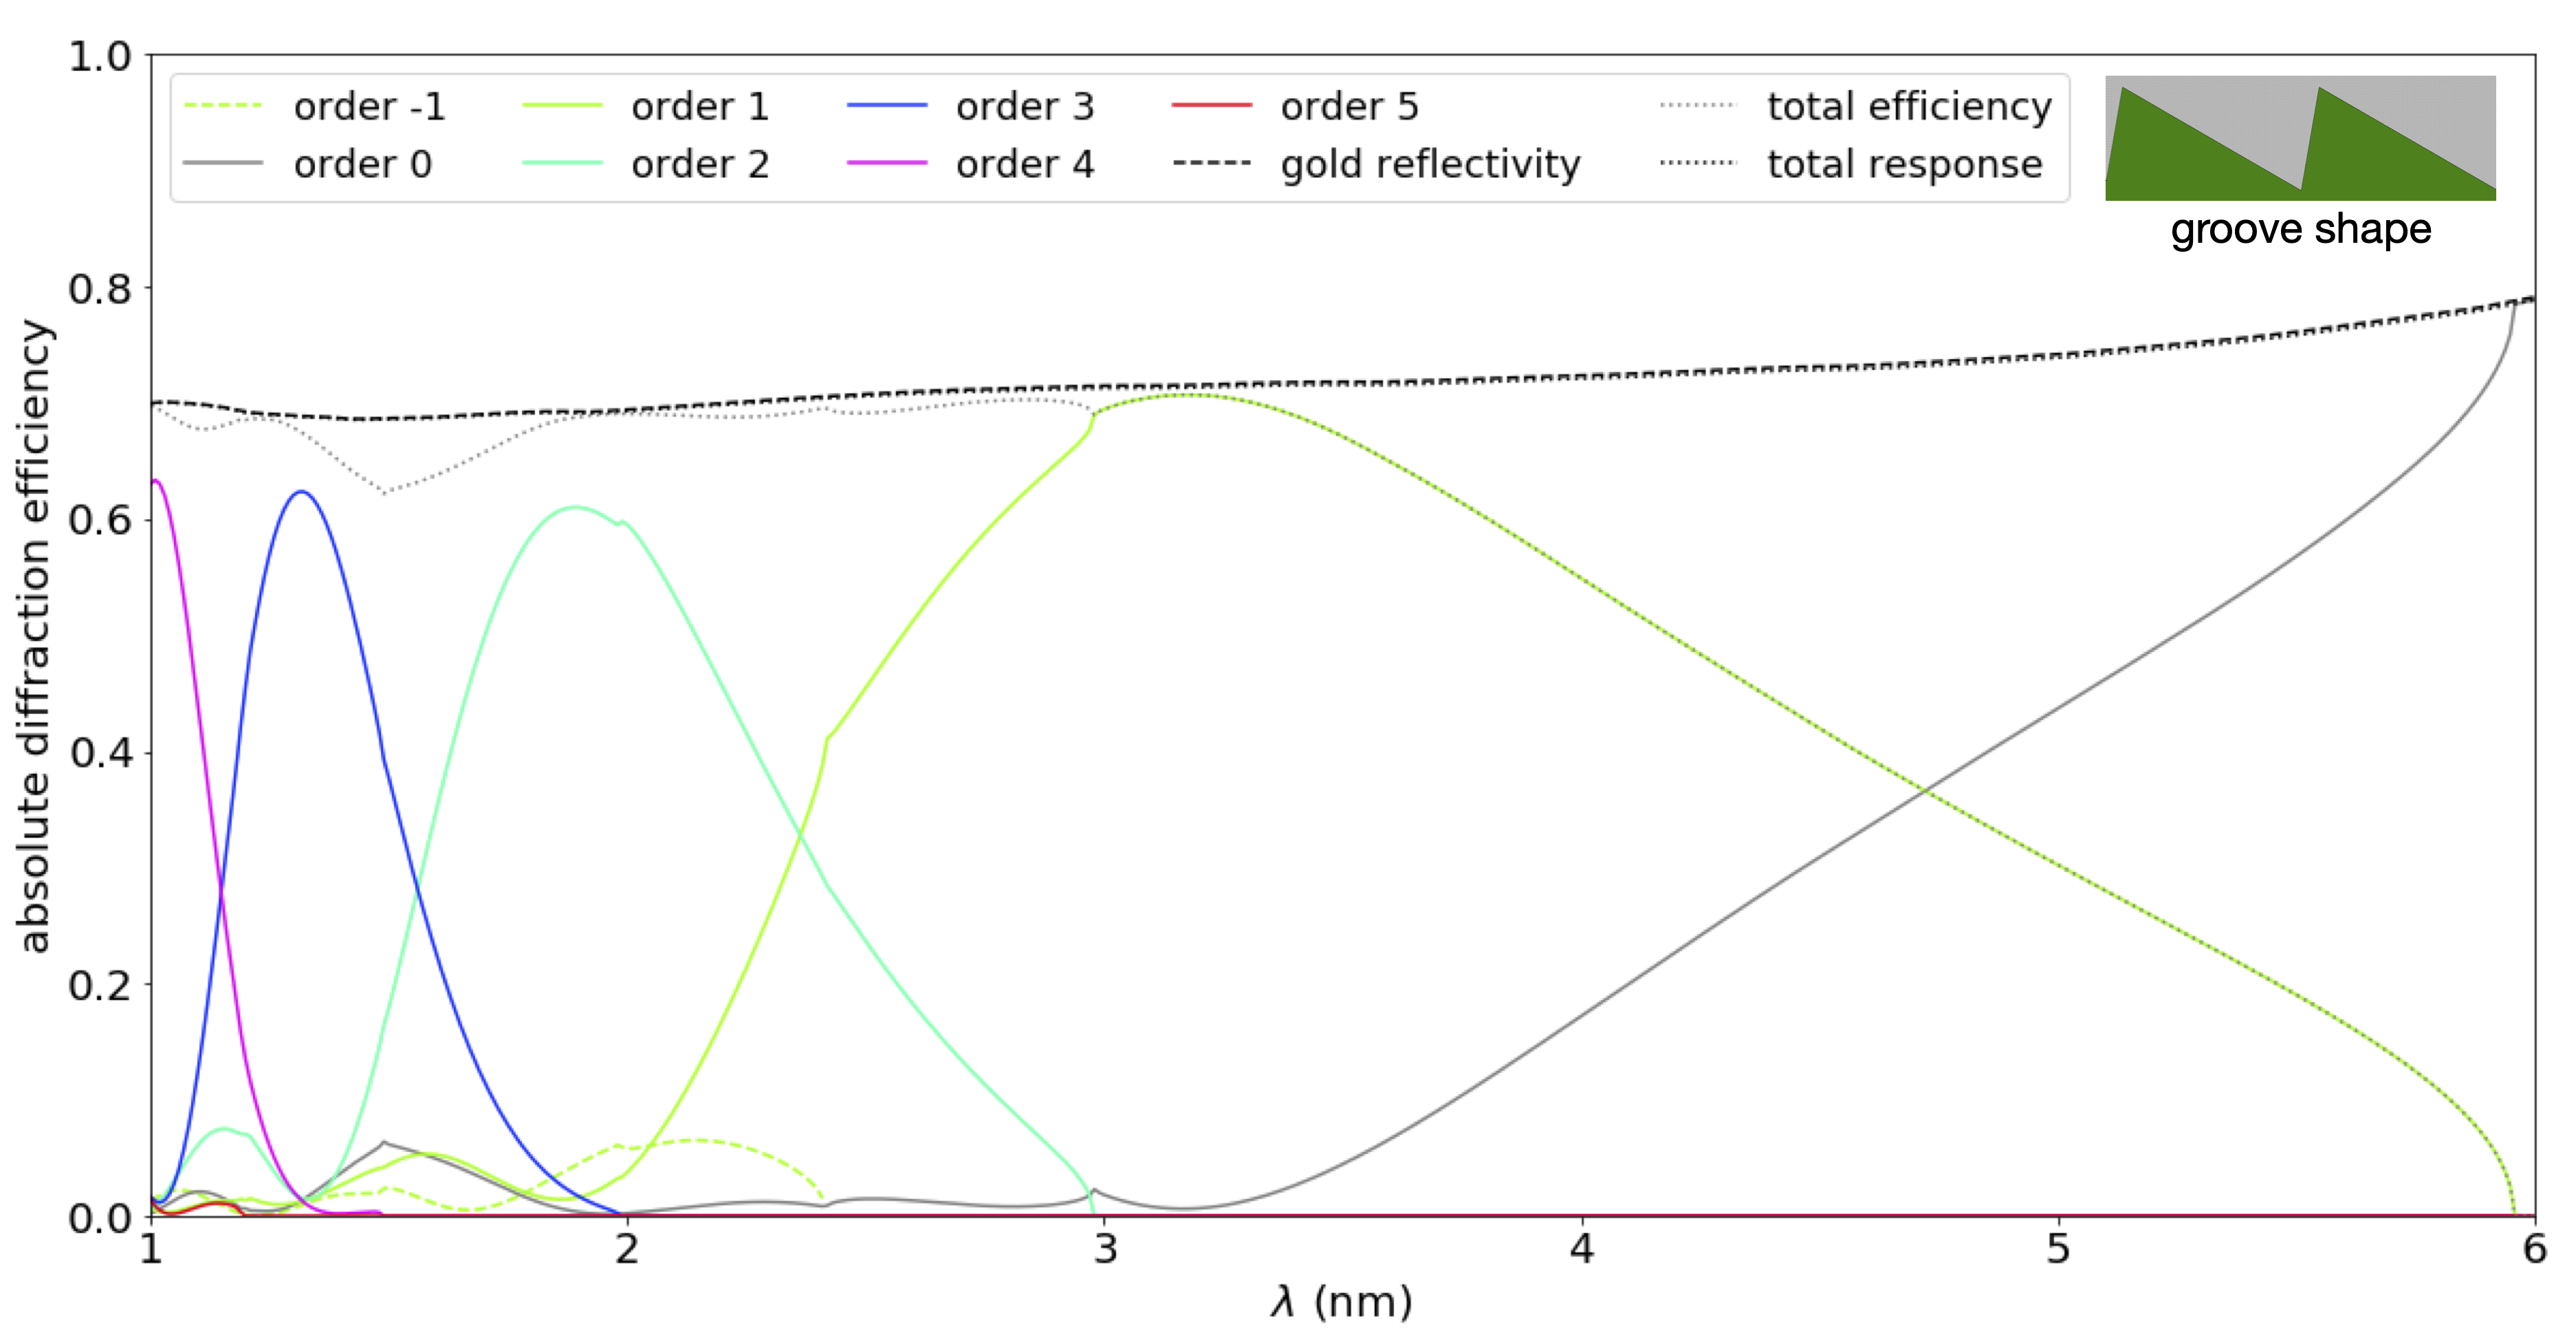
\includegraphics[scale=0.12]{Figures/au_ex.png}
% \vspace{-2mm}
% \caption{Example of predicted diffraction efficiency for a gold grating using \textsc{PCGrate-SX} under perfect conductivity mode}%{Example of predicted diffraction efficiency for a gold grating using \textsc{PCGrate-SX} (v.\ 6.1) under perfect conductivity mode using the same parameters as \cref{fig:pcgrate_example_perf}. The total response of the grating predicted by \textsc{PCGrate-SX} very closely matches Fresnel reflectivity of an equivalent surface at a grazing incidence angle $\zeta \equiv \arcsin \left[ \sin \left( \gamma \right) \cos \left( \delta - \alpha \right) \right]$.}\label{fig:pcgrate_example_au}
% \end{figure}
% \end{minipage}
% \hfill
% \begin{minipage}[t]{0.44\linewidth}
%\begin{figure}
% \centering
% \includegraphics[scale=0.5]{Figures/diffraction_arc26.mps}
% \caption{Definition of the polarization angle, $\theta_p$}%{Definition of the polarization angle, $\theta_p$. The projection of the incident electric field amplitude, $\mathbold{E}_0$, onto the $(x,y)$ plane is represented by the unit vector $\hat{\mathbold{E}}_{xy}$, which is aligned with $\mathbold{E}_0 - E_{0,z} \mathbold{\hat{z}}$. This vector, along with the projection of $\mathbold{k}$ onto the $(x,y)$ plane given by $\mathbold{k}_{xy} \equiv \mathbold{k} - k_z \mathbold{\hat{z}} = - k_0 \sin \left( \gamma \right) \left[ \sin \left( \alpha \right) \mathbold{\hat{x}} + \cos \left( \alpha \right) \mathbold{\hat{y}} \right]$, define the angle $\theta_p$ with $\theta_p = 0$ and $\theta_p = \pi/2$ corresponding to TE and TM polarization, respectively.}\label{fig:polarization_angle}
% \end{figure} 
% \begin{figure}
% \centering
% \includegraphics[scale=0.65]{Figures/diffraction_arc23.mps} 
% \caption{Surface-relief boundary between vacuum and dispersive medium representing functional material of reflection grating}%{Surface-relief boundary between vacuum and a dispersive medium representing the functional material of a reflection grating. With grooves aligned with the $z$-direction as in \cref{fig:grating_angles}, the cross-sectional profile, $\mathcal{P}$ (shown as a dashed line), of a grating with a groove spacing $d$ is described by the periodic function $g(x)$ confined to $0 \leq y \leq h$, where $h$ is the groove depth. The unit vector $\mathbold{\hat{n}}_{\mathcal{P}}(x)$ describes the direction normal to grating surface at a position $x$.}\label{fig:grating_boundary_def} 
% \end{figure}
% \end{minipage}
%\end{frame}


\section{Grating Fabrication by Thermally-Activated Selective Topography Equilibration (TASTE)} 
\subsection{Process Development for TASTE \& Grating Prototype Fabrication}

\begin{frame}{Grating Fabrication by TASTE}
\begin{minipage}[t]{0.63\linewidth}
\vspace{-3mm}
\begin{figure}
 \centering
 \includegraphics[scale=0.6]{Figures/reflow_fab1.mps}
 \includegraphics[scale=0.6]{Figures/reflow_fab2.mps}
 \includegraphics[scale=0.6]{Figures/reflow_fab3.mps}
 \includegraphics[scale=0.6]{Figures/reflow_fab4.mps}
 \caption{Outline of a traditional thermal reflow process}%{Outline of a traditional thermal reflow process. EBL can be used to pattern a laminar structure in resist such that a dose $D$ causes exposed resist with reduced molecular weight, $M_w'$, to be etched away during wet development. With the remaining, unexposed resist having a uniform average molecular weight, $M_{w,0}$, and a glass-liquid transition temperature, $T_g$, thermal reflow can be induced for $T \gtrapprox T_g + \SI{50}{\celsius}$, which causes the laminar structure to become molten so that it evolves toward a convex topography with an energy-optimal contact angle, $\theta$, according to a time-dependent, viscoelastic creep process.}\label{fig:reflow_diagram}
 \end{figure} 
 \end{minipage}
 \hfill
 \begin{minipage}[t]{0.36\linewidth}
 \textbf{EBL and thermal reflow}
 \begin{itemize}
  \item Electron exposure with \emph{dose} $D$ reduces \emph{molecular weight} $M_w$ via chain scission %High-energy electron exposure
  \item Exposed resist is soluble in developer, clear to substrate
  \item Remaining resist has \emph{glass-liquid transition temperature} $T_g$ 
  \begin{itemize}
    \item {\footnotesize Depends on $M_w$}
    \item {\footnotesize $\SI{100}{\celsius} \lessapprox T_g \lessapprox \SI{130}{\celsius}$ for PMMA}
  \end{itemize}
  \item $T \gtrapprox T_g + \SI{50}{\celsius}$ thermal treatment causes molten resist to equilibrate slowly into energetically-favorable, convex topography
 \end{itemize}
 %\vspace{-2mm}
 %\begin{block}{\footnotesize \emph{Contact angle}}
 %\centering
 %$\cos \left( \theta \right) = \frac{\alpha_{\text{s-a}} - \alpha_{\text{s-r}}}{\alpha_{\text{r-a}}}$
 %\end{block}
 \vspace{5mm}
 \centering{\footnotesize \emph{cf.\@} Kirchner, et al.~(2014)}
 \end{minipage}
\end{frame}

\begin{frame}{Grating Fabrication by TASTE}
\begin{minipage}[t]{0.63\linewidth}
\vspace{-3mm}
\begin{figure}
 \centering
 \includegraphics[scale=0.6]{Figures/taste_fab1.mps}
 \includegraphics[scale=0.6]{Figures/taste_fab2.mps}
 \includegraphics[scale=0.6]{Figures/taste_fab3.mps}
 \includegraphics[scale=0.6]{Figures/taste_fab4.mps}
 %\includegraphics[scale=0.6]{Figures/taste_fab5.mps} %thermally-activated selective topography equilibration (TASTE)
 \caption{Properties of GEBL-processed resist processed that enable \emph{thermally-activated selective topography equilibration (TASTE)}}%{Physical properties of PMMA resist processed by GEBL that enable TASTE. Dose-modulated electron exposure gives rise to a lateral gradient in $M_w$ so that varying resist thicknesses result from $M_w$-dependent etch rates that occur during wet development. The GEBL-fabricated structure also exhibits a lateral gradient in $T_g$, thereby enabling selective thermal reflow at a temperature $T_{g,0} > T > T_{g,1}$ that smooths the exposed staircase steps into a quasi-linear slope. The end result emulates a blazed grating with a groove spacing $d$ and a blaze angle $\delta$.}\label{fig:TASTE_diagram}
 \end{figure}
 \end{minipage}
  \hfill 
 \begin{minipage}[t]{0.36\linewidth}
 \textbf{Grayscale EBL (GEBL)}
 \begin{itemize}
  \item Dose-modulated electron exposure imparts lateral $M_w$ gradient% \newline $\implies$ $D_1 < D_2 < D_3$ yields $M_{w,1} > M_{w,2} > M_{w,3}$} %\newline $\implies$ stepped topography results from $M_w$-dependent etch rates} %in wet development
  \begin{itemize}
    \item[$\implies$] $D_1 < D_2 < D_3$ yields $M_{w,1} > M_{w,2} > M_{w,3}$
  \end{itemize}
  \item $M_w$-dependent etch rates give rise to stepped structure %\newline $\implies$ $M_{w,1} > M_{w,2} > M_{w,3}$ yields $h_1 > h_2 > h_3 = 0$ for timed wet development}
  \begin{itemize}
    \item[$\implies$] {$M_{w,1} > M_{w,2} > M_{w,3}$ yields $h_1 > h_2 > h_3 = 0$ \newline (timed wet development)}
  \end{itemize}
  \item GEBL structure exhibits lateral gradient in $T_g$ %\newline $\implies$ $M_{w,0} > M_{w,1} > M_{w,2}$ yields $T_{g,0} > T_{g,1} > T_{g,2}$}
  \begin{itemize}
    \item[$\implies$] $M_{w,0} > M_{w,1} > M_{w,2}$ yields $T_{g,0} > T_{g,1} > T_{g,2}$
    \item[$\implies$] \textbf{Enables selective thermal reflow} at $T_{g,0} > T > T_{g,1}$
  \end{itemize}
  \item Need experimentally-determined \emph{resist-contrast curve}: $h(D)$
  %\item {GEBL structure exhibits lateral gradient in $T_g$ \newline $\implies$ enables selective thermal reflow at $T_{g,0} > T > T_{g,1}$}
  %\item {Exposed staircase steps smooth into quasi-linear slope \newline $\implies$ end result emulates blazed grating with a $d$ and $\delta$}
 \end{itemize}
  \vspace{2mm}
 \centering{\footnotesize \emph{cf.\@} Schleunitz, et al.~(2014)}
 \end{minipage}
\end{frame}

\begin{frame}{Grating Fabrication by TASTE}
\begin{minipage}[t]{0.48\linewidth}
 \begin{figure}
 \centering
 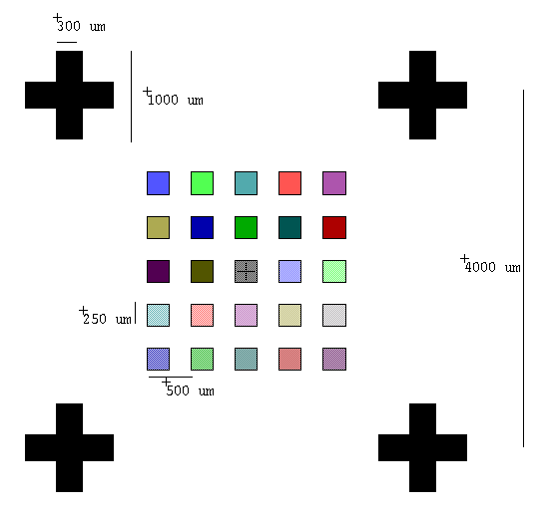
\includegraphics[scale=0.45]{Figures/contrast_pattern.png}
 \caption{CAD (\textsc{Tanner L-Edit}) for resist-contrast data collection}%{CAD layout for resist-contrast data collection prepared using the \textsc{Tanner L-Edit} software package where an array of \num{25} squares, each \SI{250}{\um} in width, is assigned to a range of values using \textsc{Layout BEAMER}.}\label{fig:dose_layout}
 \end{figure}
 \end{minipage}
 %\hfill
 \begin{minipage}[t]{0.48\linewidth}
  \begin{figure}
 \centering
 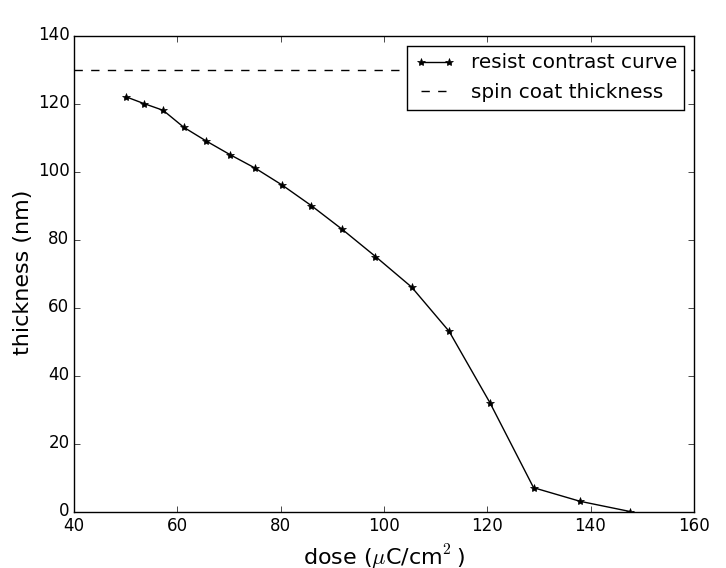
\includegraphics[scale=0.45]{Figures/resist_contrast.png}
 \caption{Resist contrast for \SI{130}{\nm}-thick, $\SI{950}{\kilogram\per\mole}$ PMMA using 1:1 MIBK/IPA for \SI{2}{\minute}, IPA for \SI{30}{\second}}%{Resist contrast for \SI{130}{\nm}-thick PMMA with $M_w = \SI{950}{\kilogram\per\mole}$ developed at room temperature using 1:1 MIBK/IPA for \SI{2}{\minute} and IPA for \SI{30}{\second}: the center of each square of the pattern shown in \cref{fig:dose_layout} is measured using spectroscopic ellipsometry and a film thickness is extracted. Resist contrast is plotted as remaining resist thickness as a function of electron dose, $D$.}\label{fig:resist_contrast}
 \end{figure}
 \end{minipage}
  \vspace{-3mm}
 \centering {\footnotesize McCoy, et al. (2018)}
 %Use \textsc{Layout BEAMER} to
\end{frame}

\begin{frame}{Grating Fabrication by TASTE}
\begin{minipage}[t]{0.48\linewidth}
\textbf{GEBL process development}
\begin{itemize}
 \item Input resist-contrast data to \textsc{BEAMER 3DPEC} algorithm for \emph{proximity-effect correction (PEC)}
 \item Expose and develop test patterns for GEBL
 %\item Examine samples under AFM
 \end{itemize}
\textbf{Test patterns}
\begin{itemize}
 \item \emph{pattern A}: 6-level staircase where each step is \SI{140}{\nm} wide $\implies d = \SI{840}{\nm}$
 \item \emph{pattern B}: 4-level staircase where each step is \SI{100}{\nm} wide $\implies d = \SI{400}{\nm}$
 \item \emph{pattern C}: 4-level staircase where top step is reduced to \SI{40}{\nm}; remaining levels are \SI{120}{\nm} wide $\implies d = \SI{400}{\nm}$
 %\item \emph{pattern D}: Emulation of pattern C attained through \textsc{EBPG5200} sequencing%\footnote{This was carried out according to the pattern shown in \cref{fig:GEBL_approaches}(B), where the overlapping beams emulate doses $D$, $1.5D$ and $2D$ with $D = \SI{75}{\micro\coulomb\per\cm\squared}$ as the user-input dose.}
 \end{itemize}
 \textbf{Carry out thermal reflow experimentation}
 \begin{itemize}
  \item Explore $T$-$t$ parameter space
 \end{itemize}
 \end{minipage}
 \hfill
 \begin{minipage}[t]{0.48\linewidth}
 \vspace{-5mm}
\begin{figure}
 \centering
 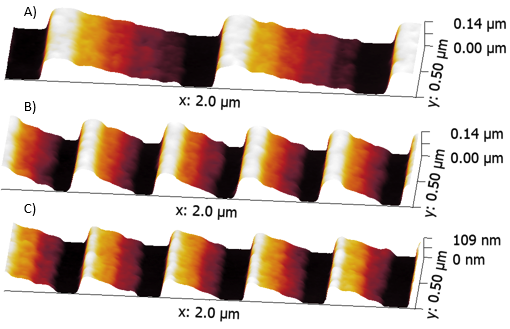
\includegraphics[scale=0.4]{Figures/GEBL_alt.png}
 \caption{AFMs of GEBL test patterns in \SI{130}{\nm}-thick PMMA}%examined under AFM%{GEBL in \SI{130}{\nm}-thick PMMA examined under AFM. Patterns A-C were attained through the standard 3DPEC approach while pattern D is a result from the \textsc{EBPG5200} sequencing approach: a) Pattern A: GEBL with 6 levels where each are \SI{140}{\nm} wide to give a \SI{840}{\nm} periodicity. b) Pattern B: GEBL with 4 levels where each are \SI{100}{\nm} wide to give a \SI{400}{\nm} periodicity. c) Pattern C: GEBL with 4 levels where the width of the top level is reduced to \SI{40}{\nm}; remaining levels are \SI{120}{\nm} wide to give a periodicity of \SI{400}{\nm}. d) Pattern D: same as pattern C but attained using EBPG sequencing.}\label{fig:GEBL_ABCD}
 \end{figure}
 \vspace{-3mm}
 \begin{figure}
 \centering
 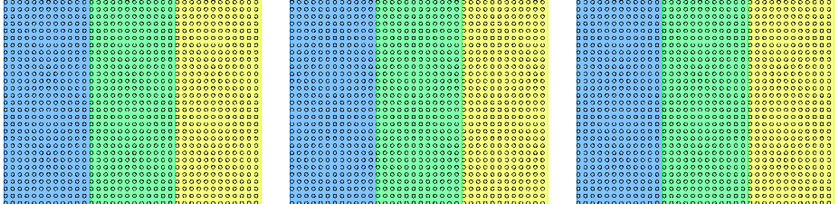
\includegraphics[scale=0.25]{Figures/GEBL_approaches_edit.png}
 \caption{\textsc{Layout BEAMER 3DPEC} for GEBL}%{Two approaches to pattern generation for GEBL: a) Experimentally-determined data for resist contrast [\emph{cf.\@} \cref{fig:resist_contrast}] are input into \textsc{Layout BEAMER} where the 3DPEC algorithm is used to generate a dose-corrected layout. Each dose is a different pattern generator shape, represented here with colorscale. b) Code for \textsc{EBPG5200} sequencing defines a custom subfield-sized pattern generator shape consisting of a series of lines and beam jumps using a fixed dose. Lines are programmed to overlap to varying degrees to emulate dose modulation achieved using the 3DPEC approach.}\label{fig:GEBL_approaches} 
 \end{figure}
 \end{minipage}
\end{frame}

\begin{frame}{Grating Fabrication by TASTE}
%\textbf{Thermal reflow experimentation}
\centering {$d = \SI{840}{\nm}$, $\delta \approx 10^{\circ}$} 
 \begin{figure}
 \centering
 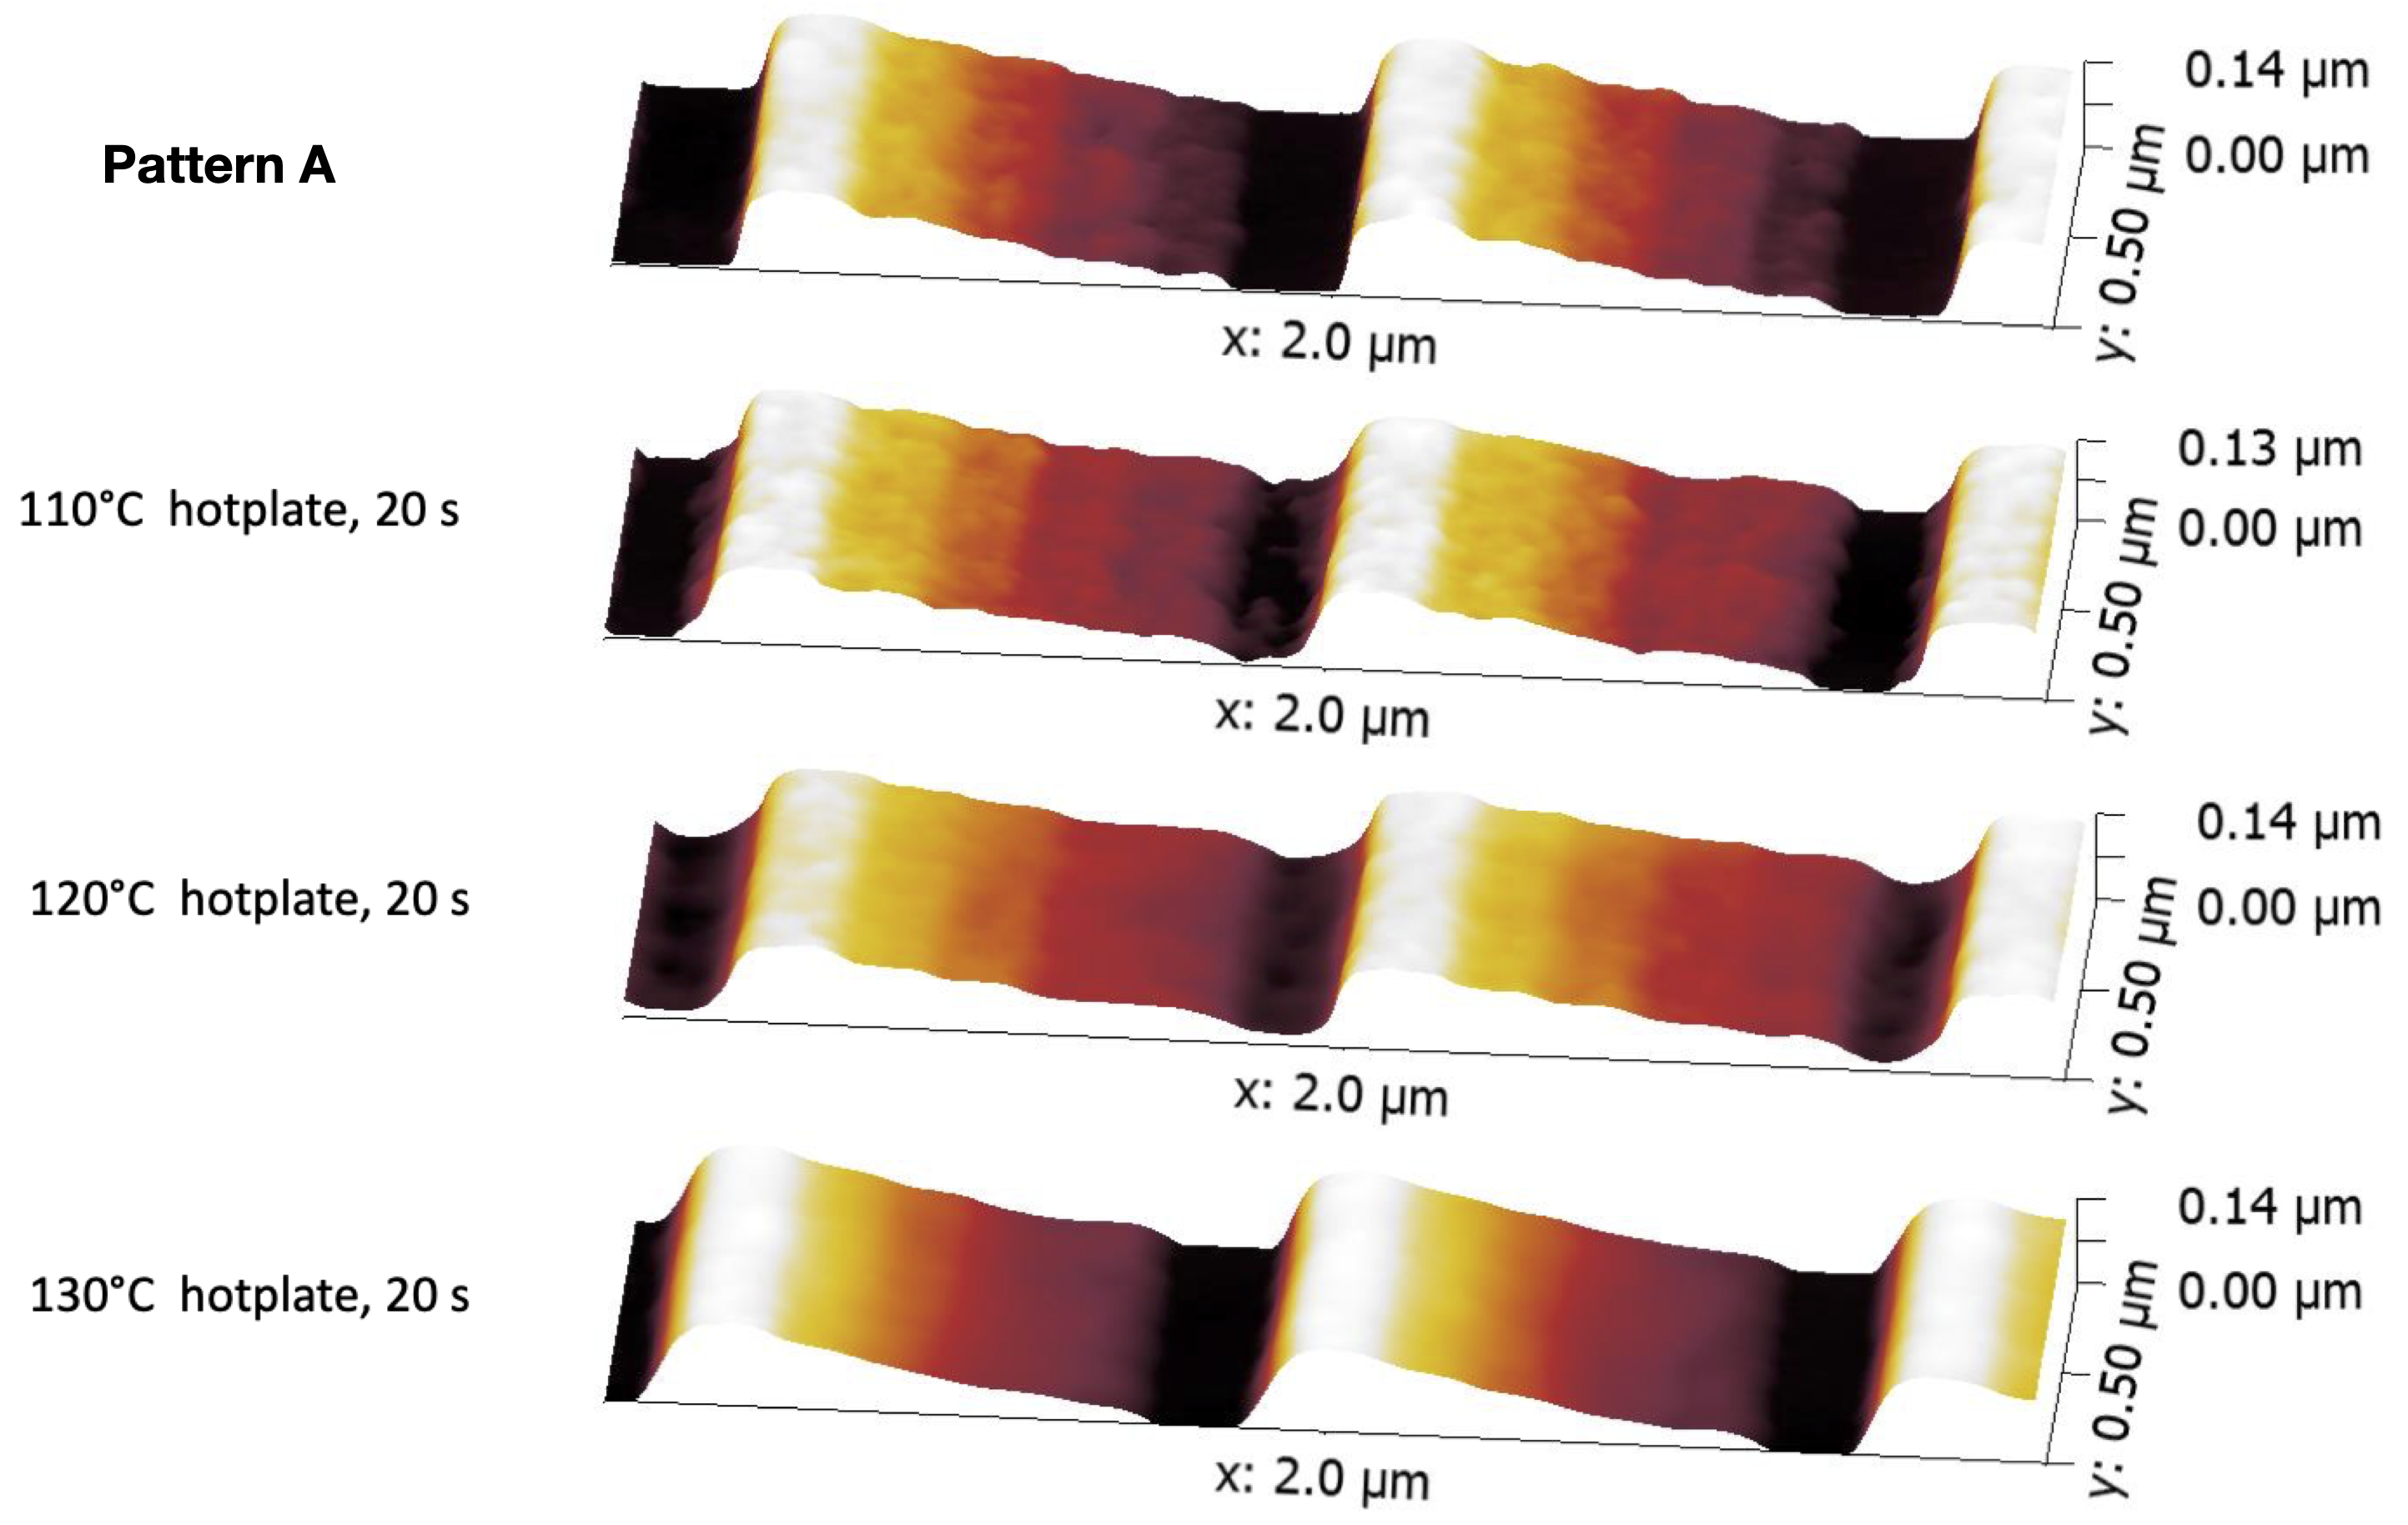
\includegraphics[scale=0.155]{Figures/A_temp_scan.png}
 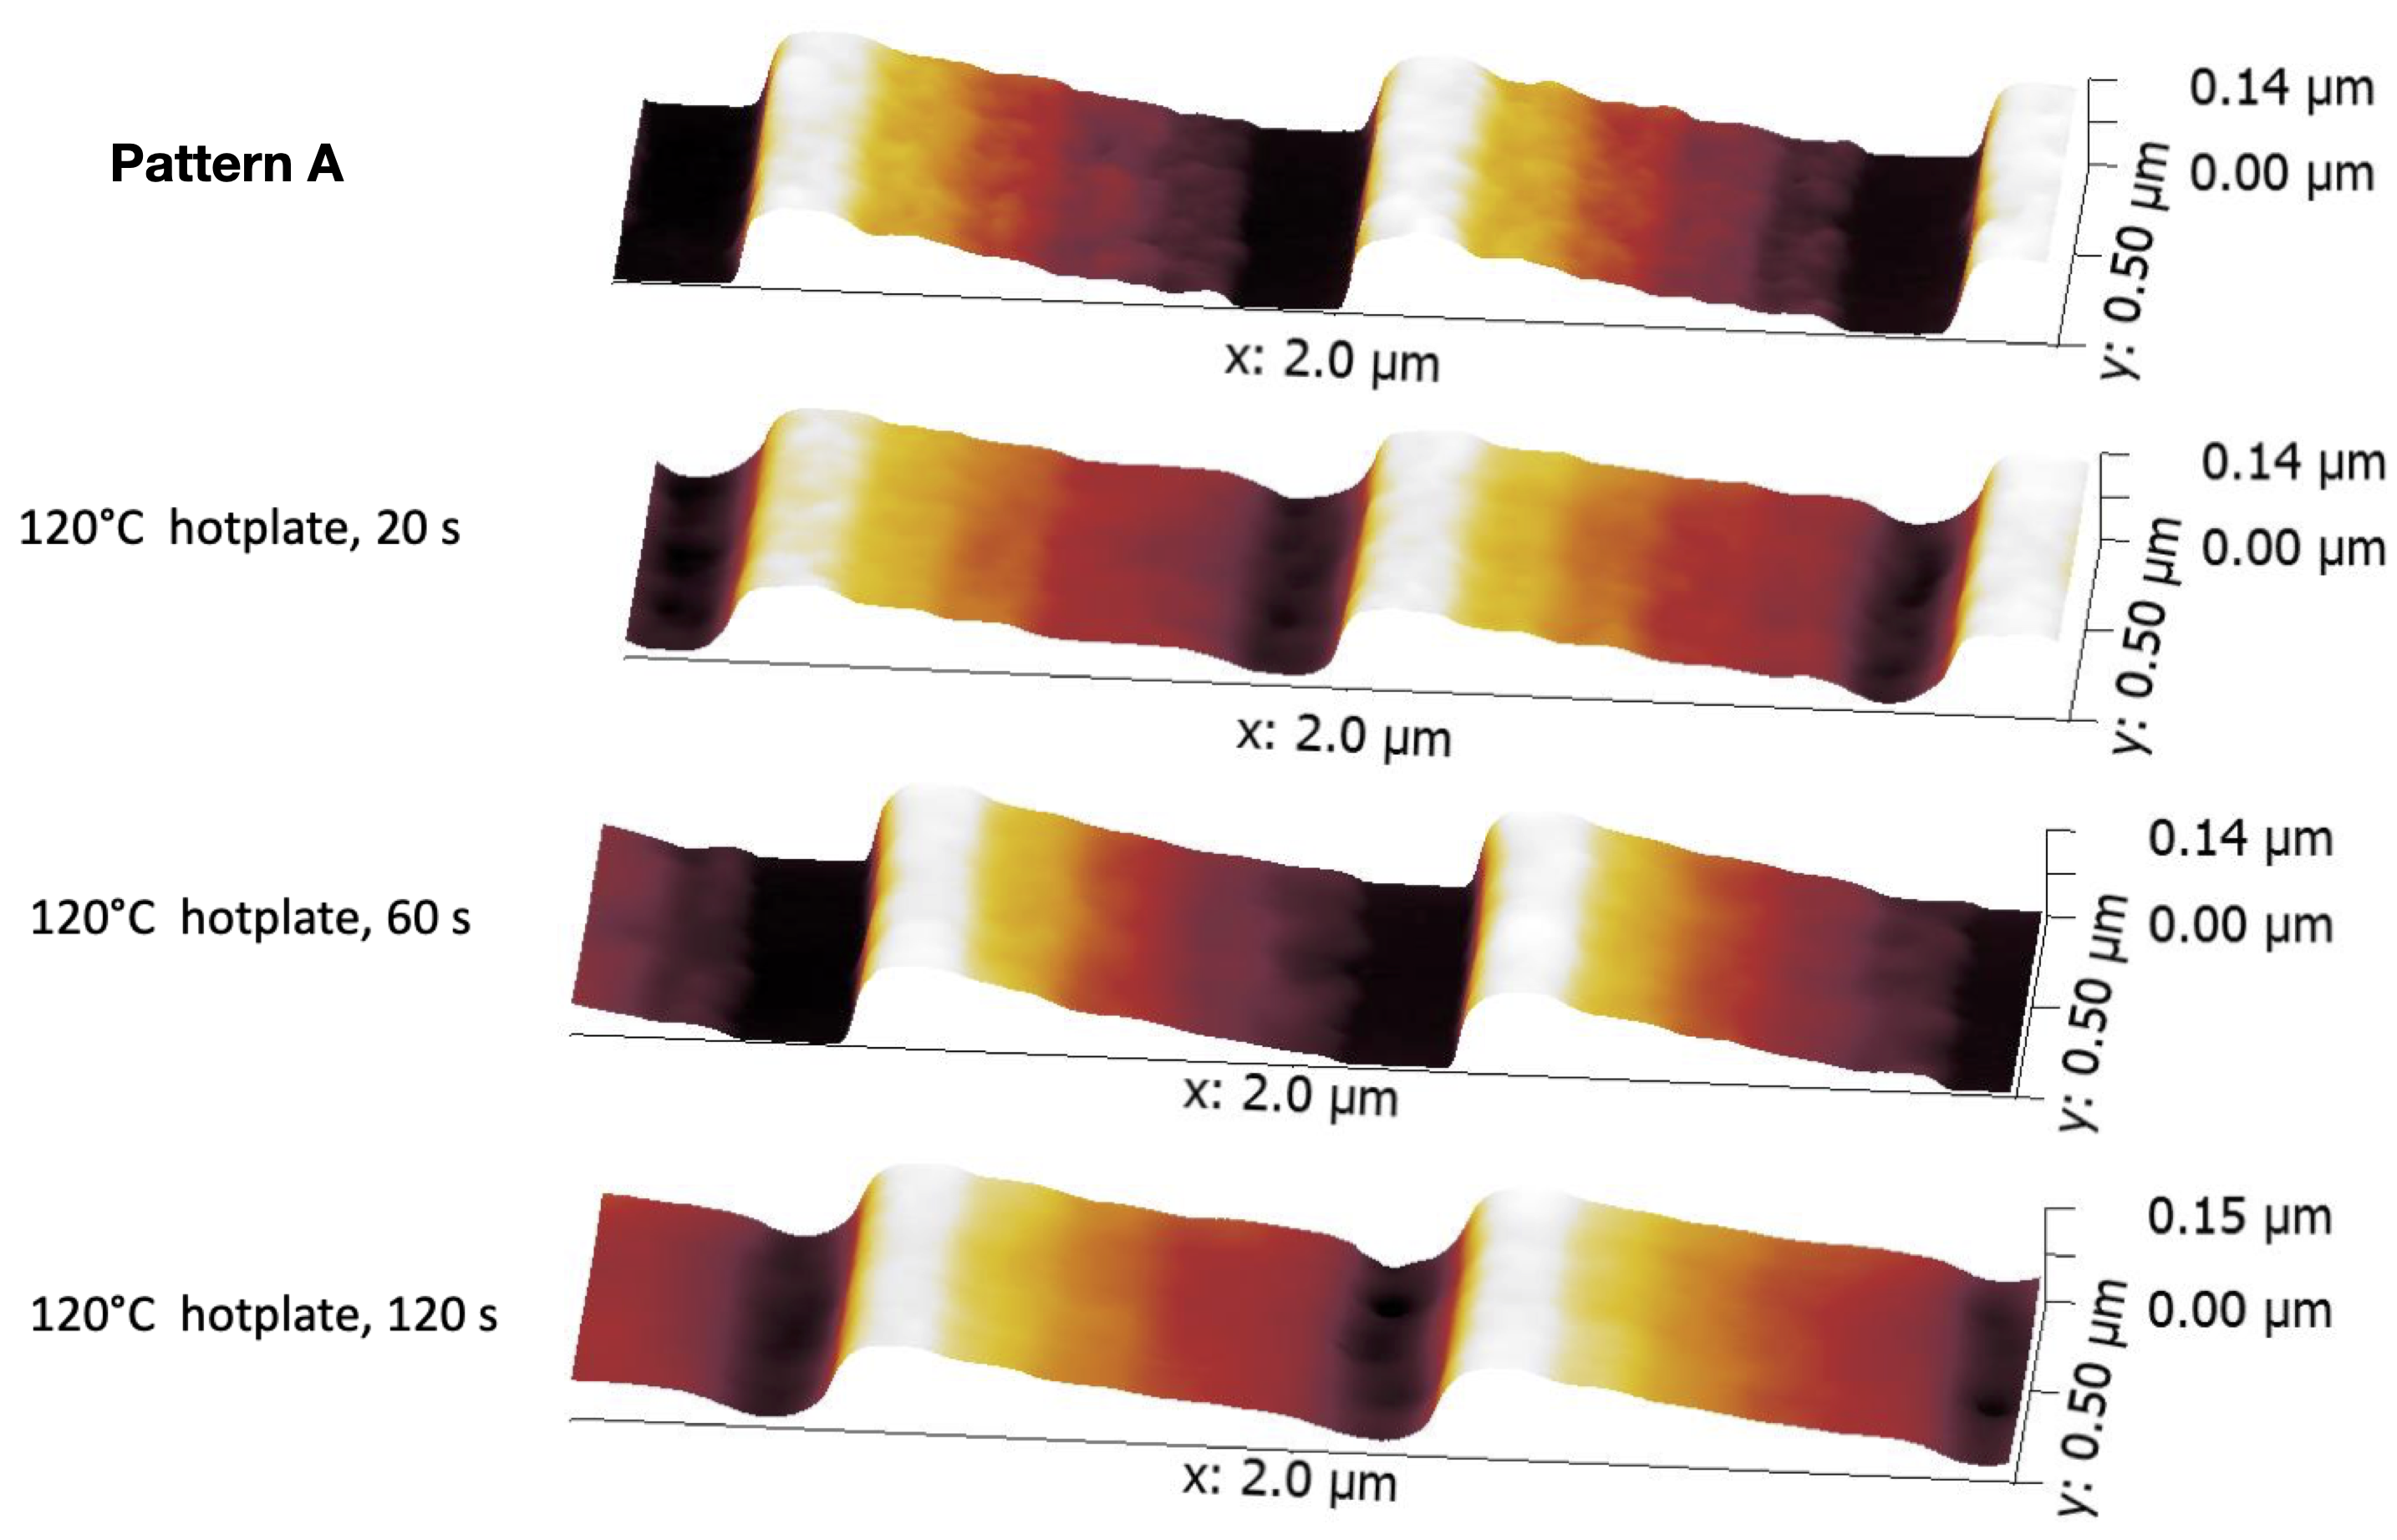
\includegraphics[scale=0.155]{Figures/A_time_scan.png}
 \caption{Thermal reflow results for pattern A as a function of $T$ (\emph{left}), as a function of $t$ (\emph{right})}%{Thermal reflow results as a function of heating temperature, $T$, for GEBL in \SI{130}{\nm}-thick PMMA with 6 levels: each are \SI{140}{\nm} wide to give $d = \SI{840}{\nm}$.}\label{fig:A_temp_scan}
 \end{figure}
 \centering {\footnotesize McCoy, et al. (2018)}
\end{frame}

\begin{frame}{Grating Fabrication by TASTE}
%\textbf{Thermal reflow experimentation}
 \centering{$d = \SI{400}{\nm}$, $\delta \approx 27^{\circ}$}
 \begin{figure}
 \centering
 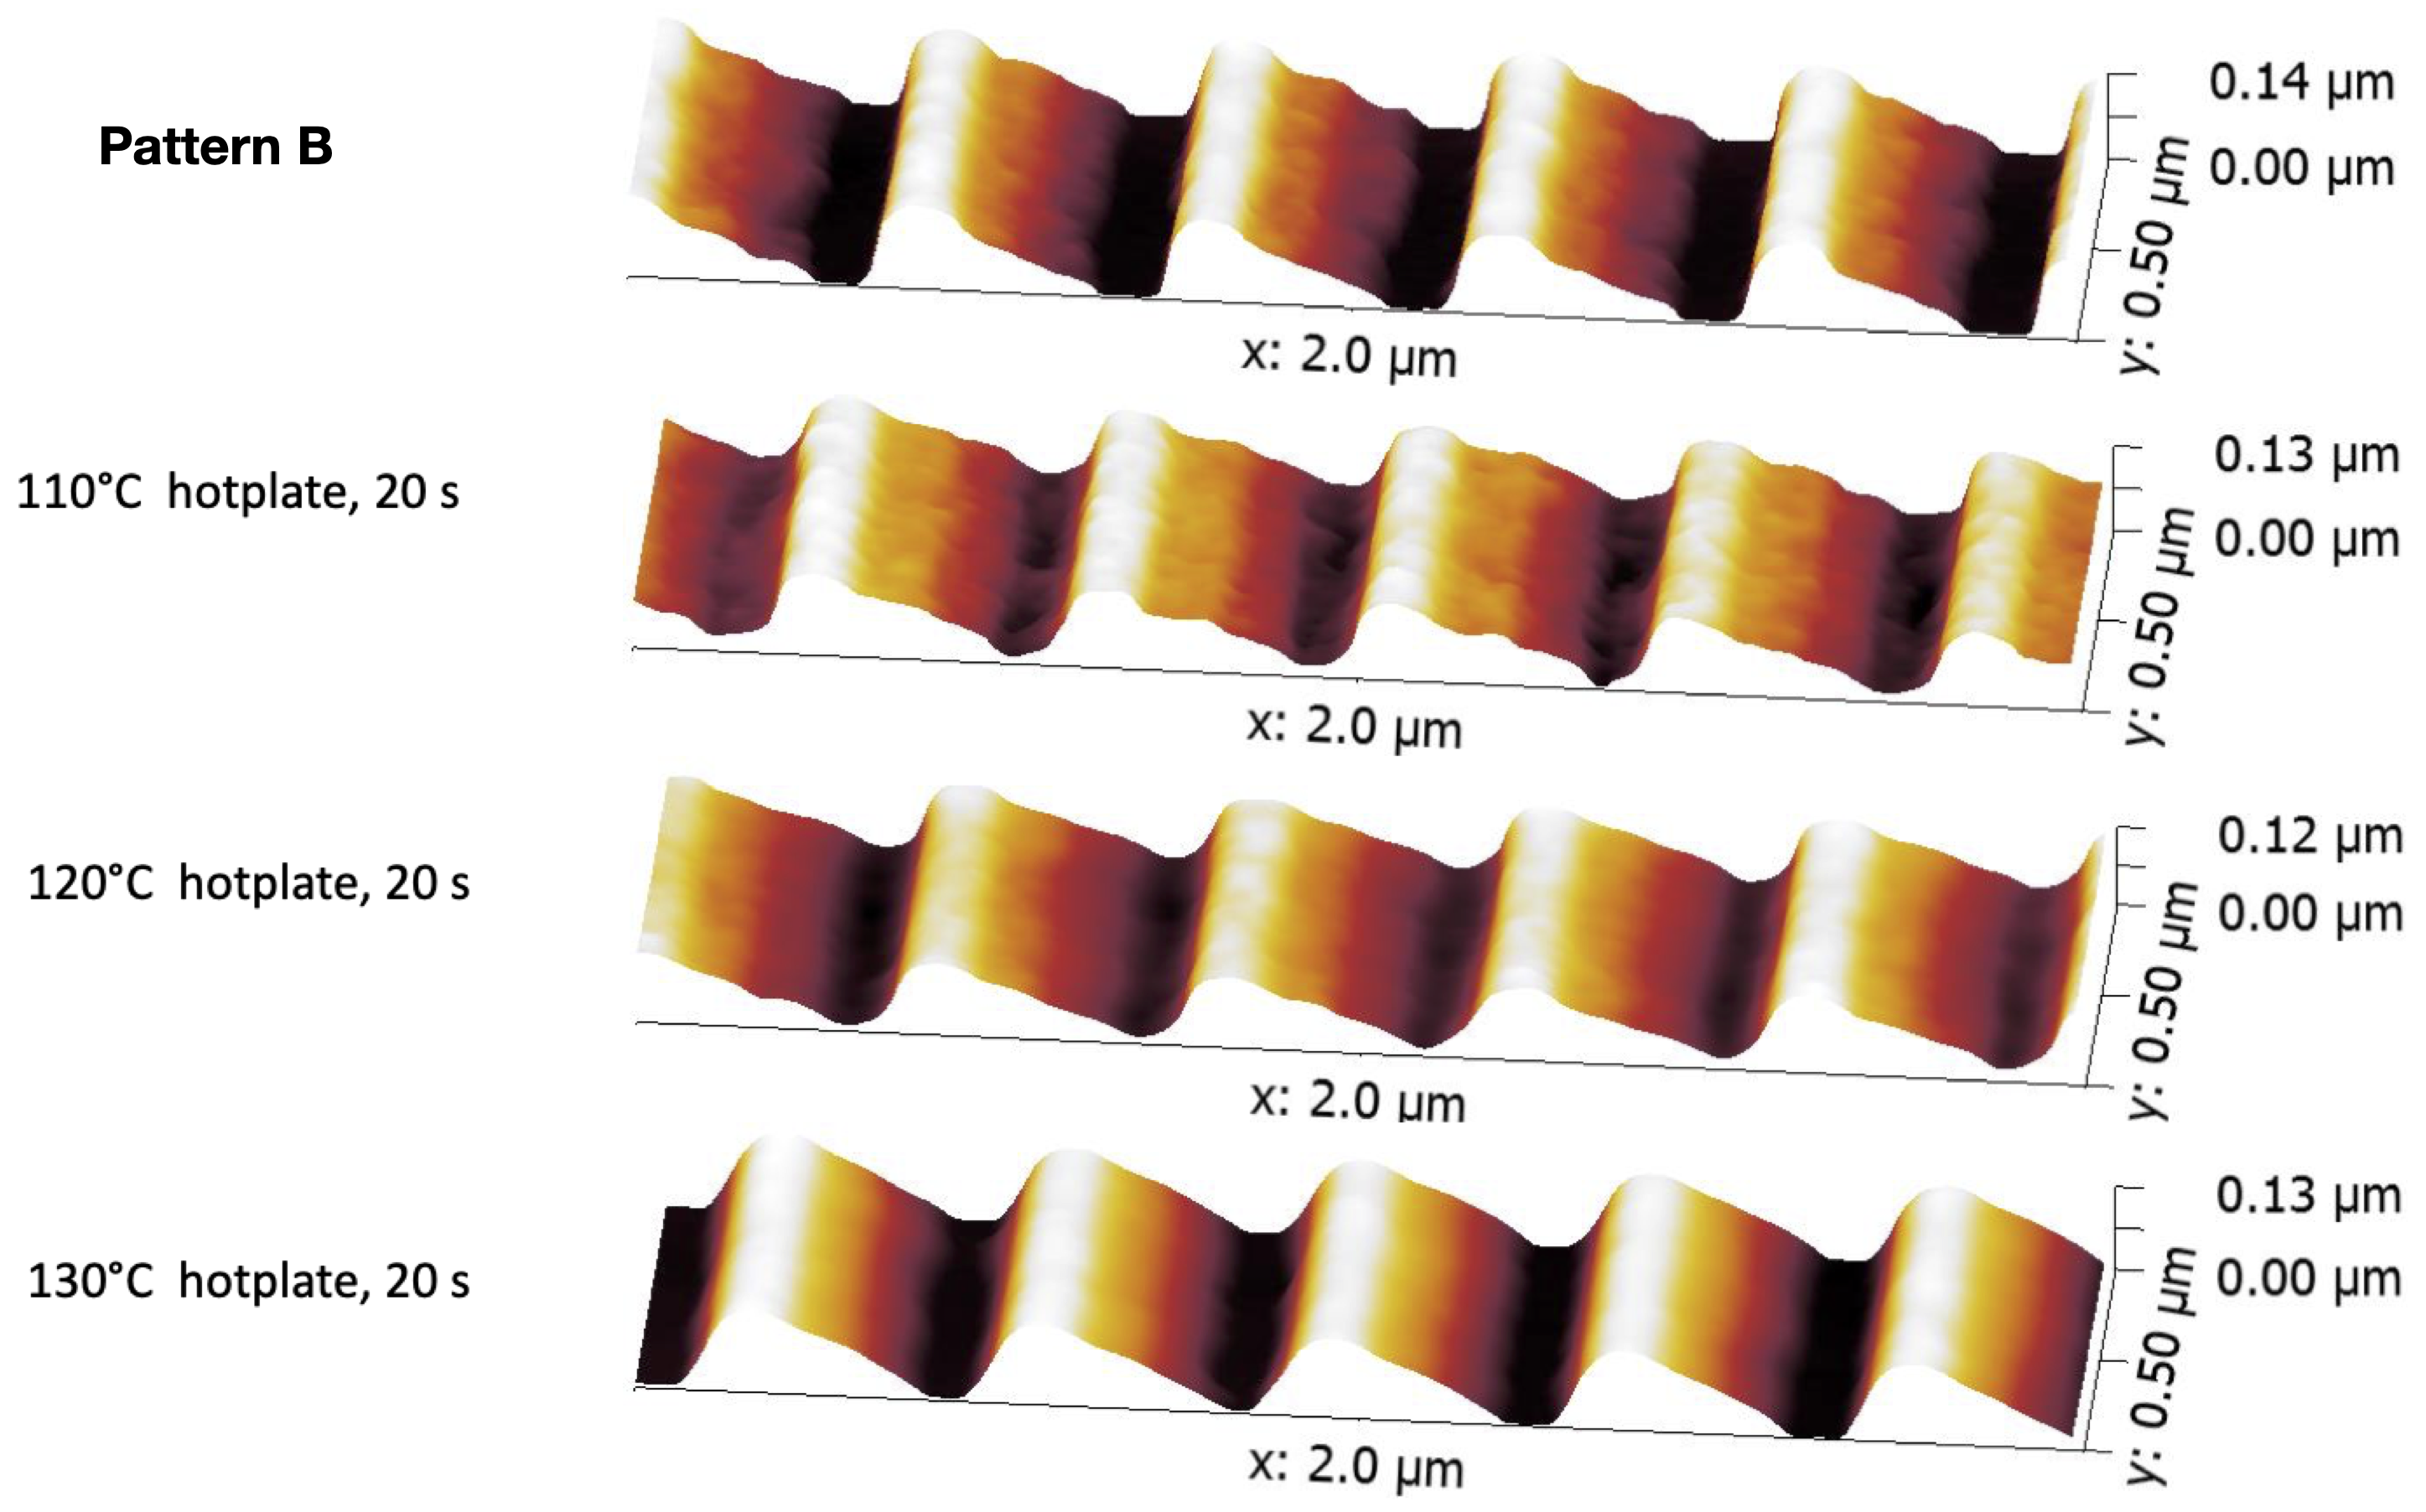
\includegraphics[scale=0.155]{Figures/B_temp_scan.png}
 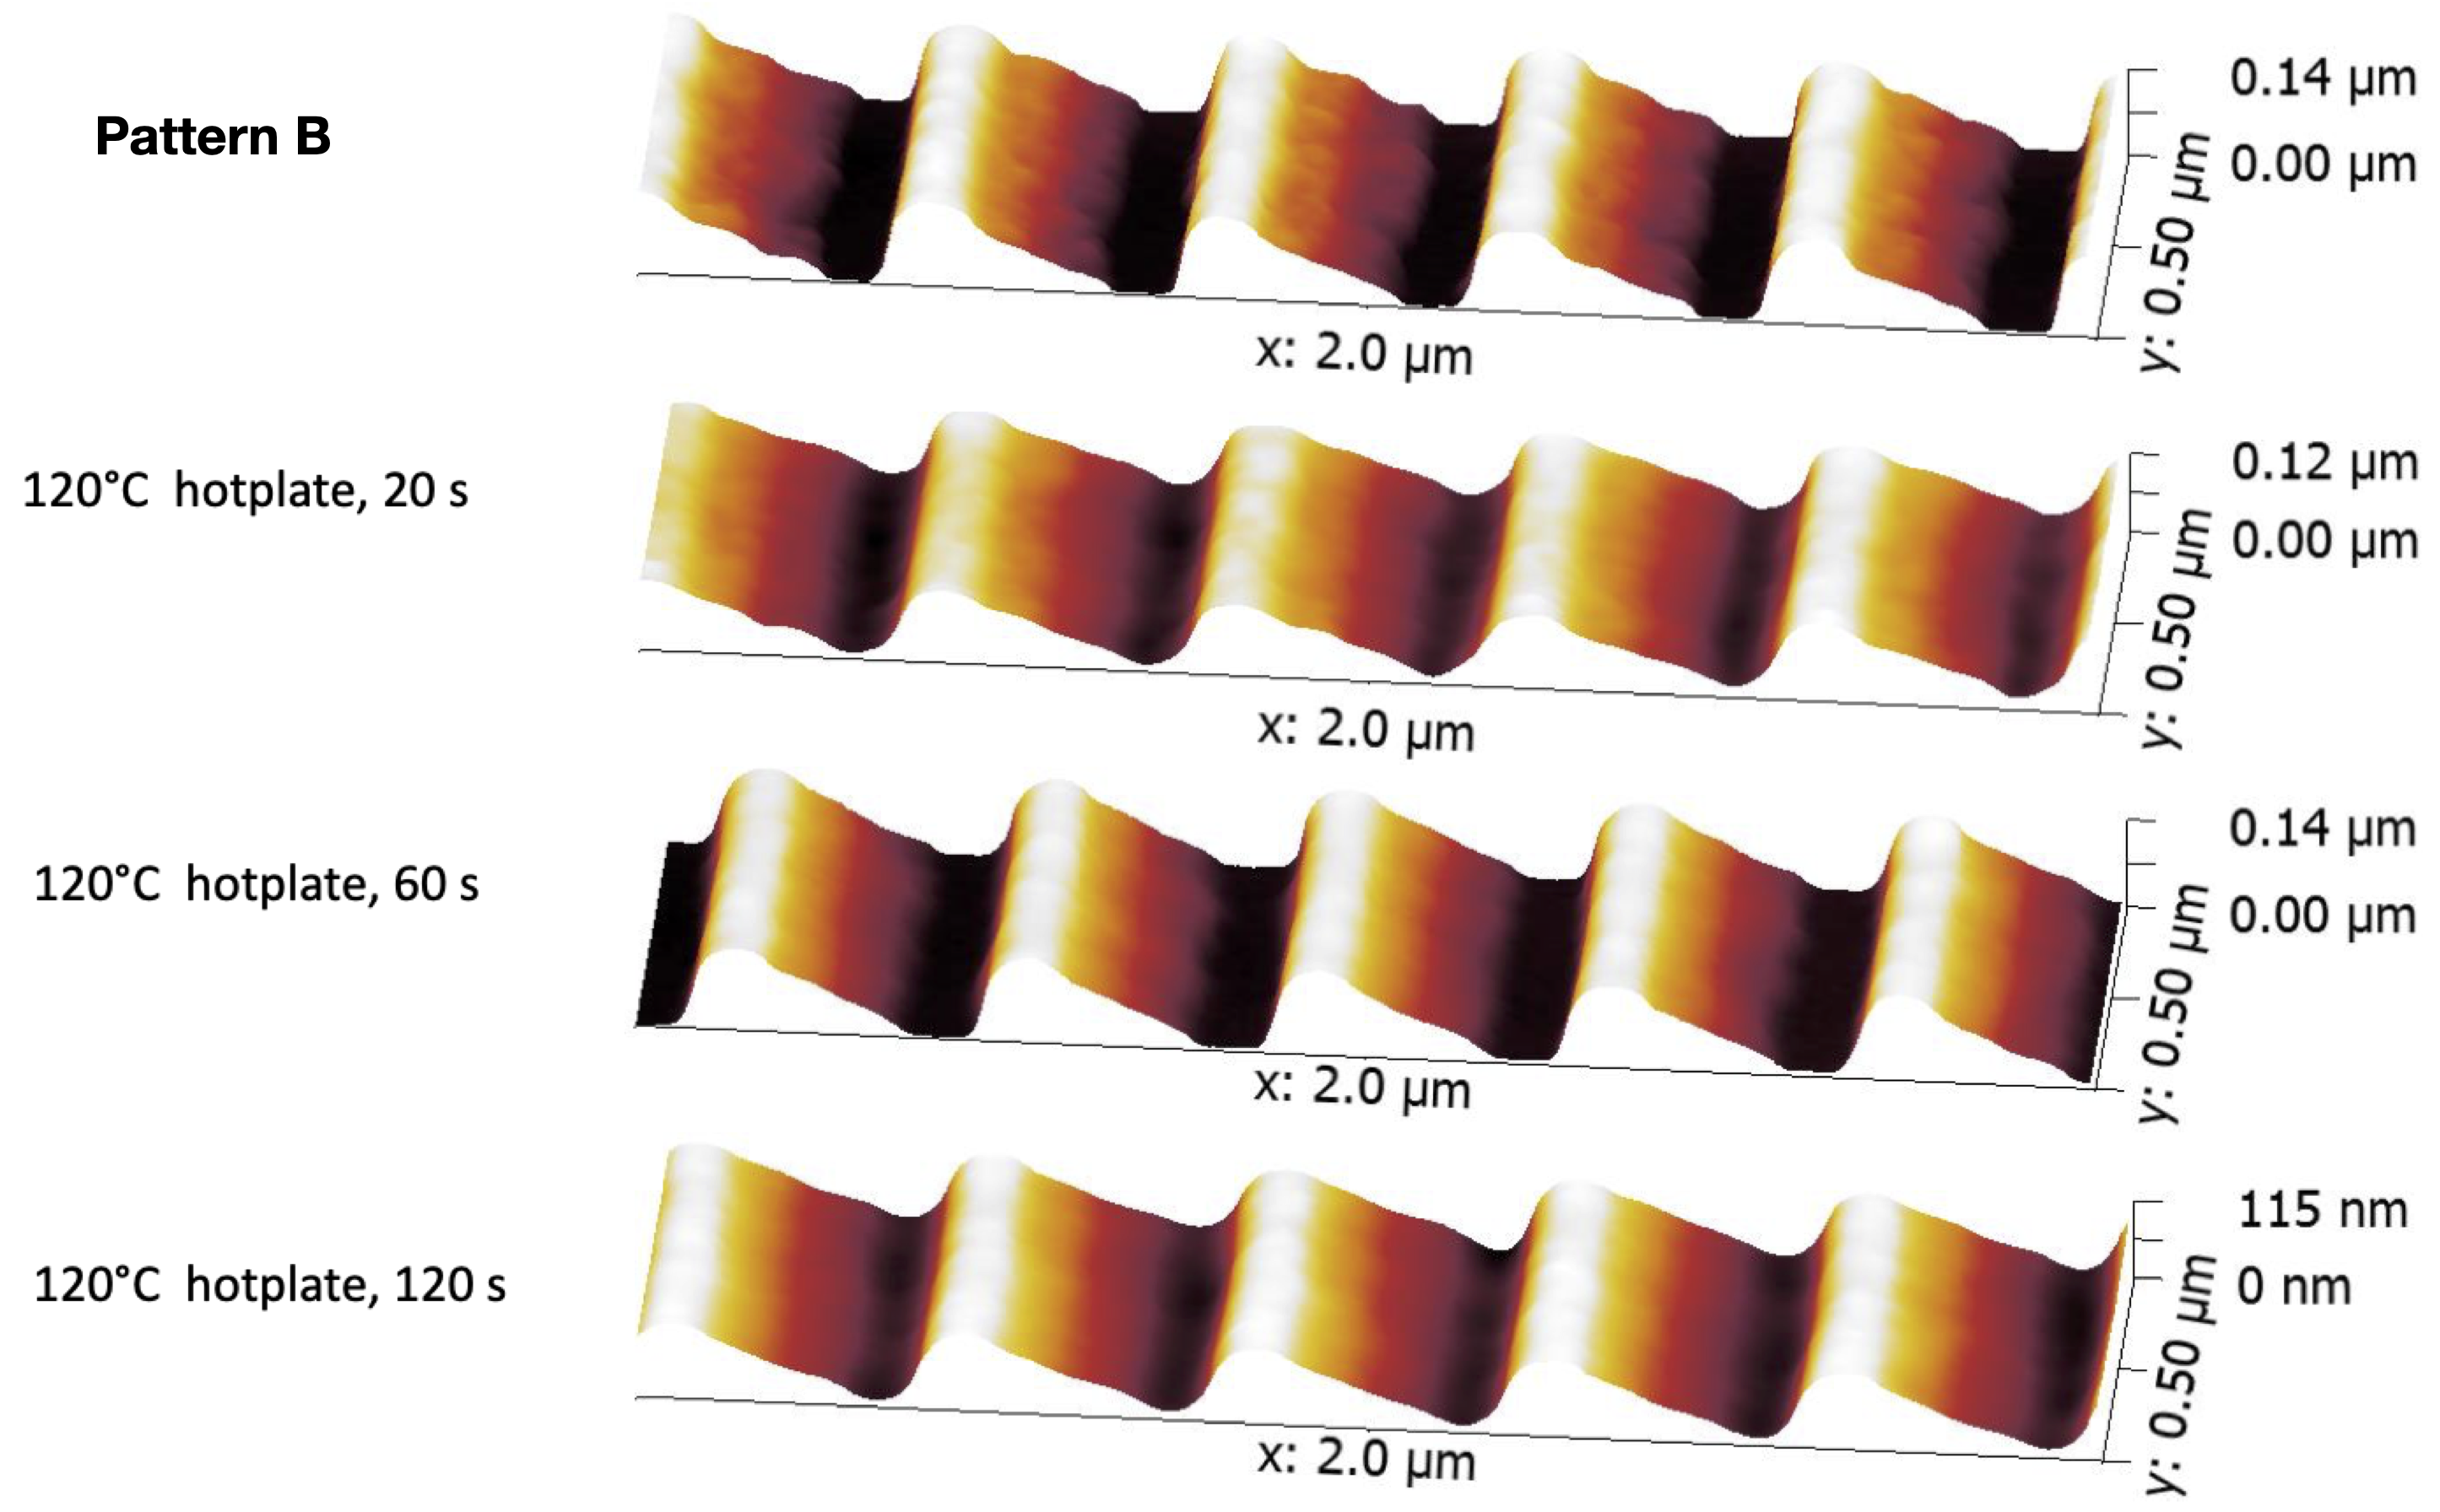
\includegraphics[scale=0.155]{Figures/B_time_scan.png}
 \caption{Thermal reflow results for pattern B as a function of $T$ (\emph{left}), as a function of $t$ (\emph{right})}%{Thermal reflow results as a function of heating temperature, $T$, for GEBL in \SI{130}{\nm}-thick PMMA with 6 levels: each are \SI{140}{\nm} wide to give $d = \SI{840}{\nm}$.}\label{fig:A_temp_scan}
 \end{figure}
 \centering {\footnotesize McCoy, et al. (2018)}
\end{frame}

%\subsection{Grating Prototype Fabrication}

\begin{frame}{Grating Fabrication by TASTE}
\begin{minipage}[t]{0.61\linewidth}
\textbf{Grating prototype}
\begin{itemize}
  \item Start from pattern B with $d = \SI{400}{\nm}$
  \item Design for $\alpha = \beta = \delta \approx 27^{\circ}$ with $\zeta = \gamma \approx 1.7^{\circ}$
  \item Pattern \SI{50}{\mm} along groove direction and \SI{7.5}{\mm} along dispersion direction to encompass soft x-ray beam
\end{itemize}
\begin{figure}
 \centering
 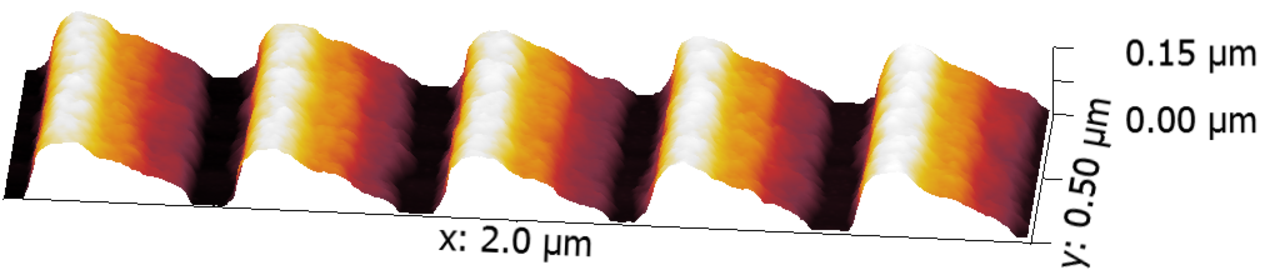
\includegraphics[scale=0.4]{Figures/grayscale_AFM.pdf}
 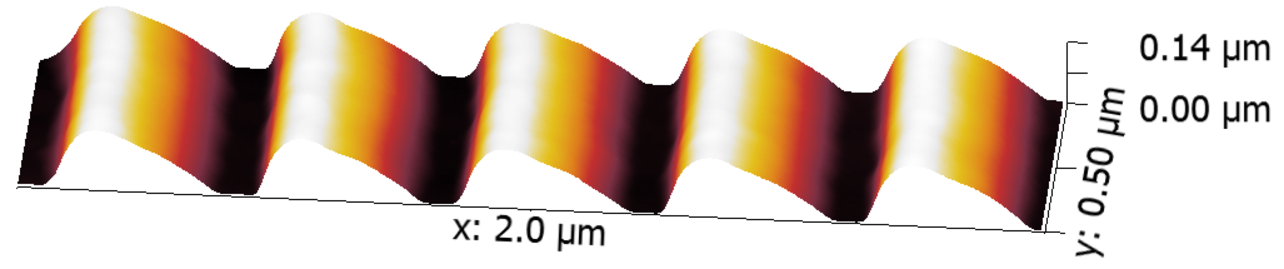
\includegraphics[scale=0.4]{Figures/reflow_AFM.pdf}
 \caption{AFM of GEBL-processed resist (\emph{top}), resist following thermal reflow at \SI{116}{\celsius} for \SI{30}{\minute} (\emph{bottom})}\label{fig:TASTE_AFMs}
 \end{figure}
 \end{minipage}
 \hfill
 \begin{minipage}[t]{0.34\linewidth}
 \begin{figure}
 \centering
 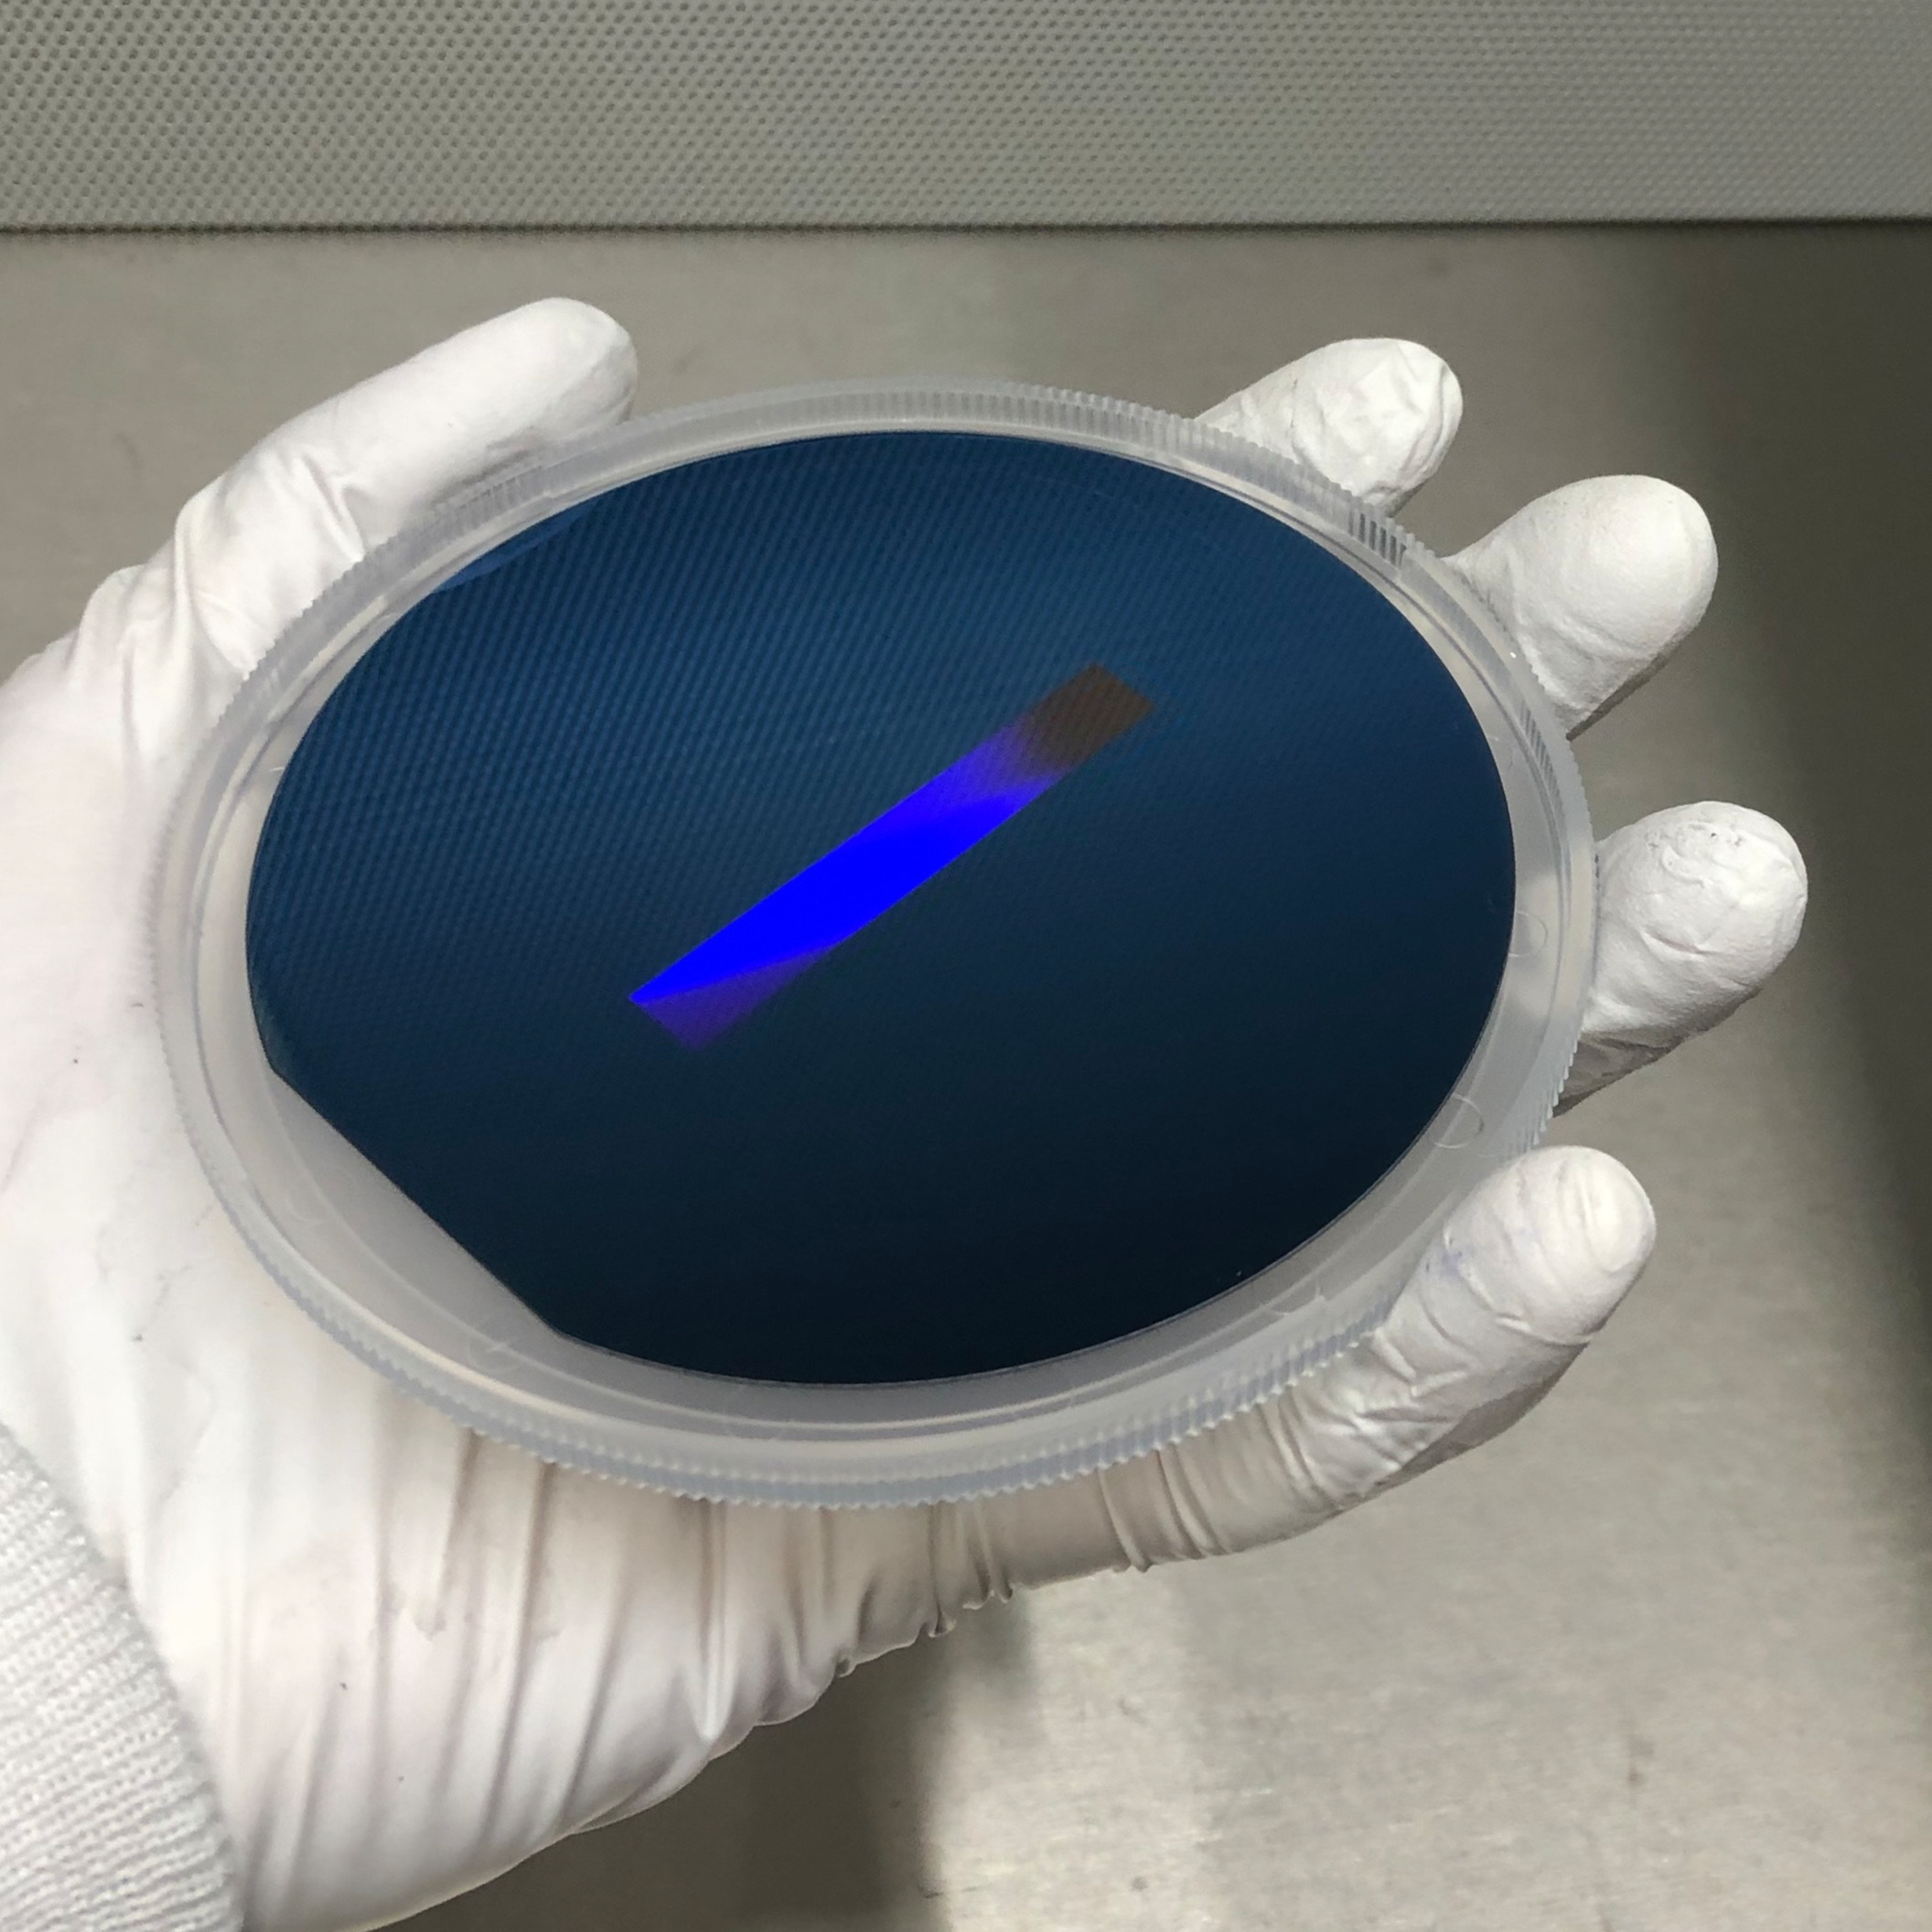
\includegraphics[scale=0.067]{Figures/uncoated_grating_photo.pdf}
 \caption{Surface-relief mold for grating prototype patterned in \SI{130}{\nm}-thick PMMA on \SI{100}{\mm}-diameter silicon wafer}\label{fig:uncoated_grating_pic} %using TASTE. %The grating measures \SI{50}{\mm} in the groove direction and \SI{7.5}{\mm} in the dispersion direction.
 \end{figure}
 \vspace{-3mm}
 \centering {\footnotesize McCoy, et al. (2020a)}
 \end{minipage}
\end{frame}

\begin{frame}{Grating Fabrication by TASTE}
\begin{minipage}[t]{0.58\linewidth}
\vspace{-3mm}
\begin{figure}
 \centering
 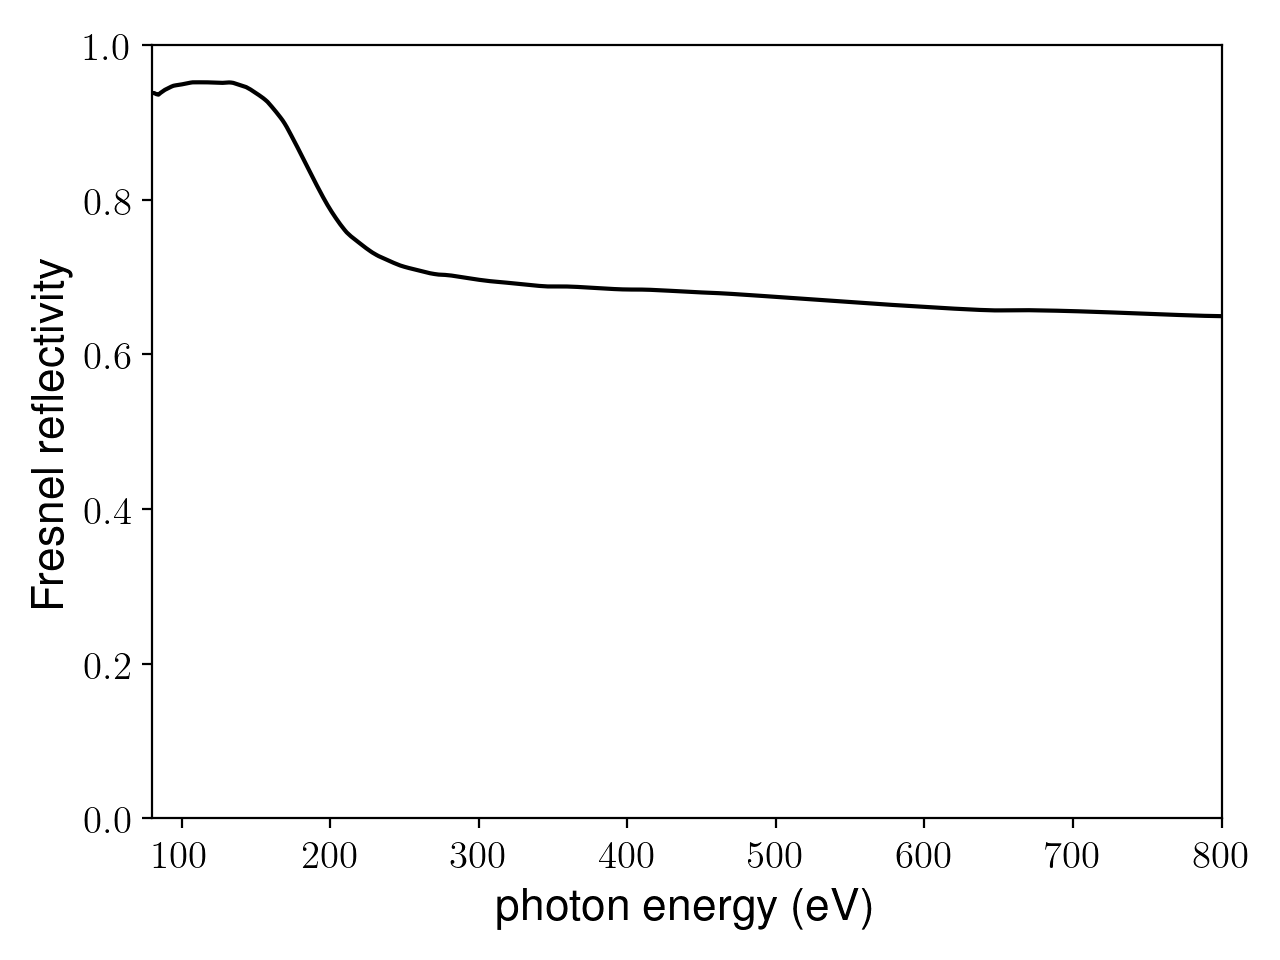
\includegraphics[scale=0.27]{Figures/reflectivity.png}
 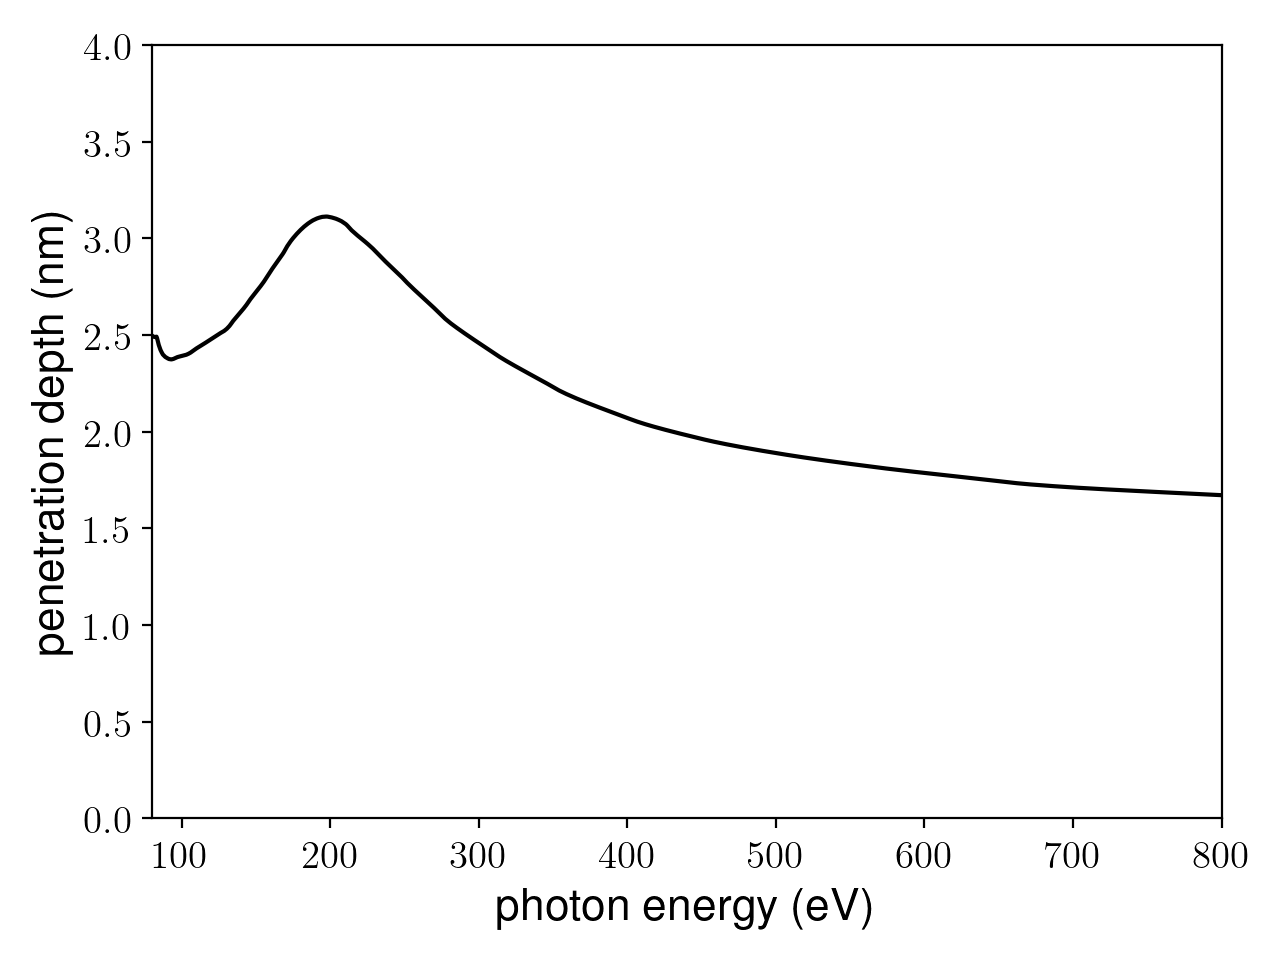
\includegraphics[scale=0.27]{Figures/attn_depth.png}
 \caption{$\mathcal{R}_F$ and $\mathcal{D}_{\perp}$ for thick slab of gold for nominal test geometry}%{Fresnel reflectivity, $\mathcal{R}_F$, and penetration depth, $\mathcal{D}_{\perp}$, in a thick slab of gold at $\zeta = 1.7^{\circ}$ over $\SI{80}{\electronvolt} <  \mathcal{E}_{\gamma} < \SI{800}{\electronvolt}$ (data obtained from CXRO).}\label{fig:Au_refl_attn} %($\mathcal{R}_F$ given by \cref{eq:ch3_fres_refl}) %($\mathcal{D}_{\perp}$ given by \cref{eq:ch3_pene_dep}) 
 \end{figure}
 \vspace{-5mm}
\begin{figure}
 \centering
 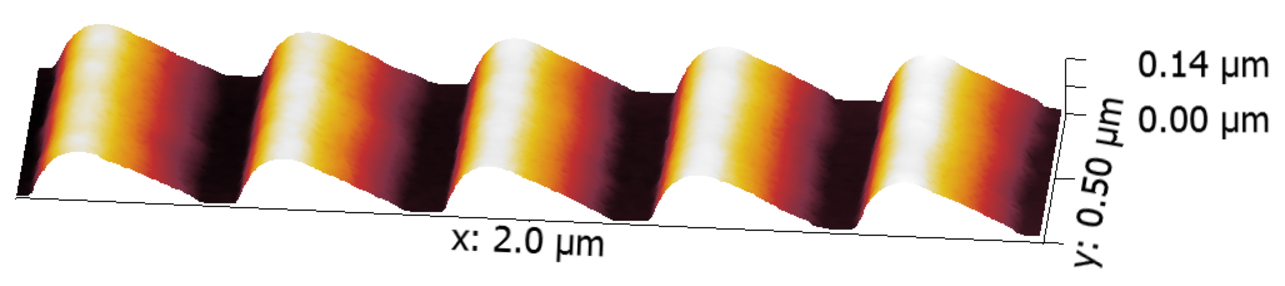
\includegraphics[scale=0.4]{Figures/coating_AFM.pdf}
 \caption{AFM of prototype grooves following EBPVD of gold using titanium as adhesion layer on PMMA}\label{fig:coating_AFM}
 \end{figure}
 \end{minipage}
 \hspace{5mm}%\hfill
 \begin{minipage}[t]{0.36\linewidth}
 \vspace{-4mm}
\begin{figure}
 %\centering
 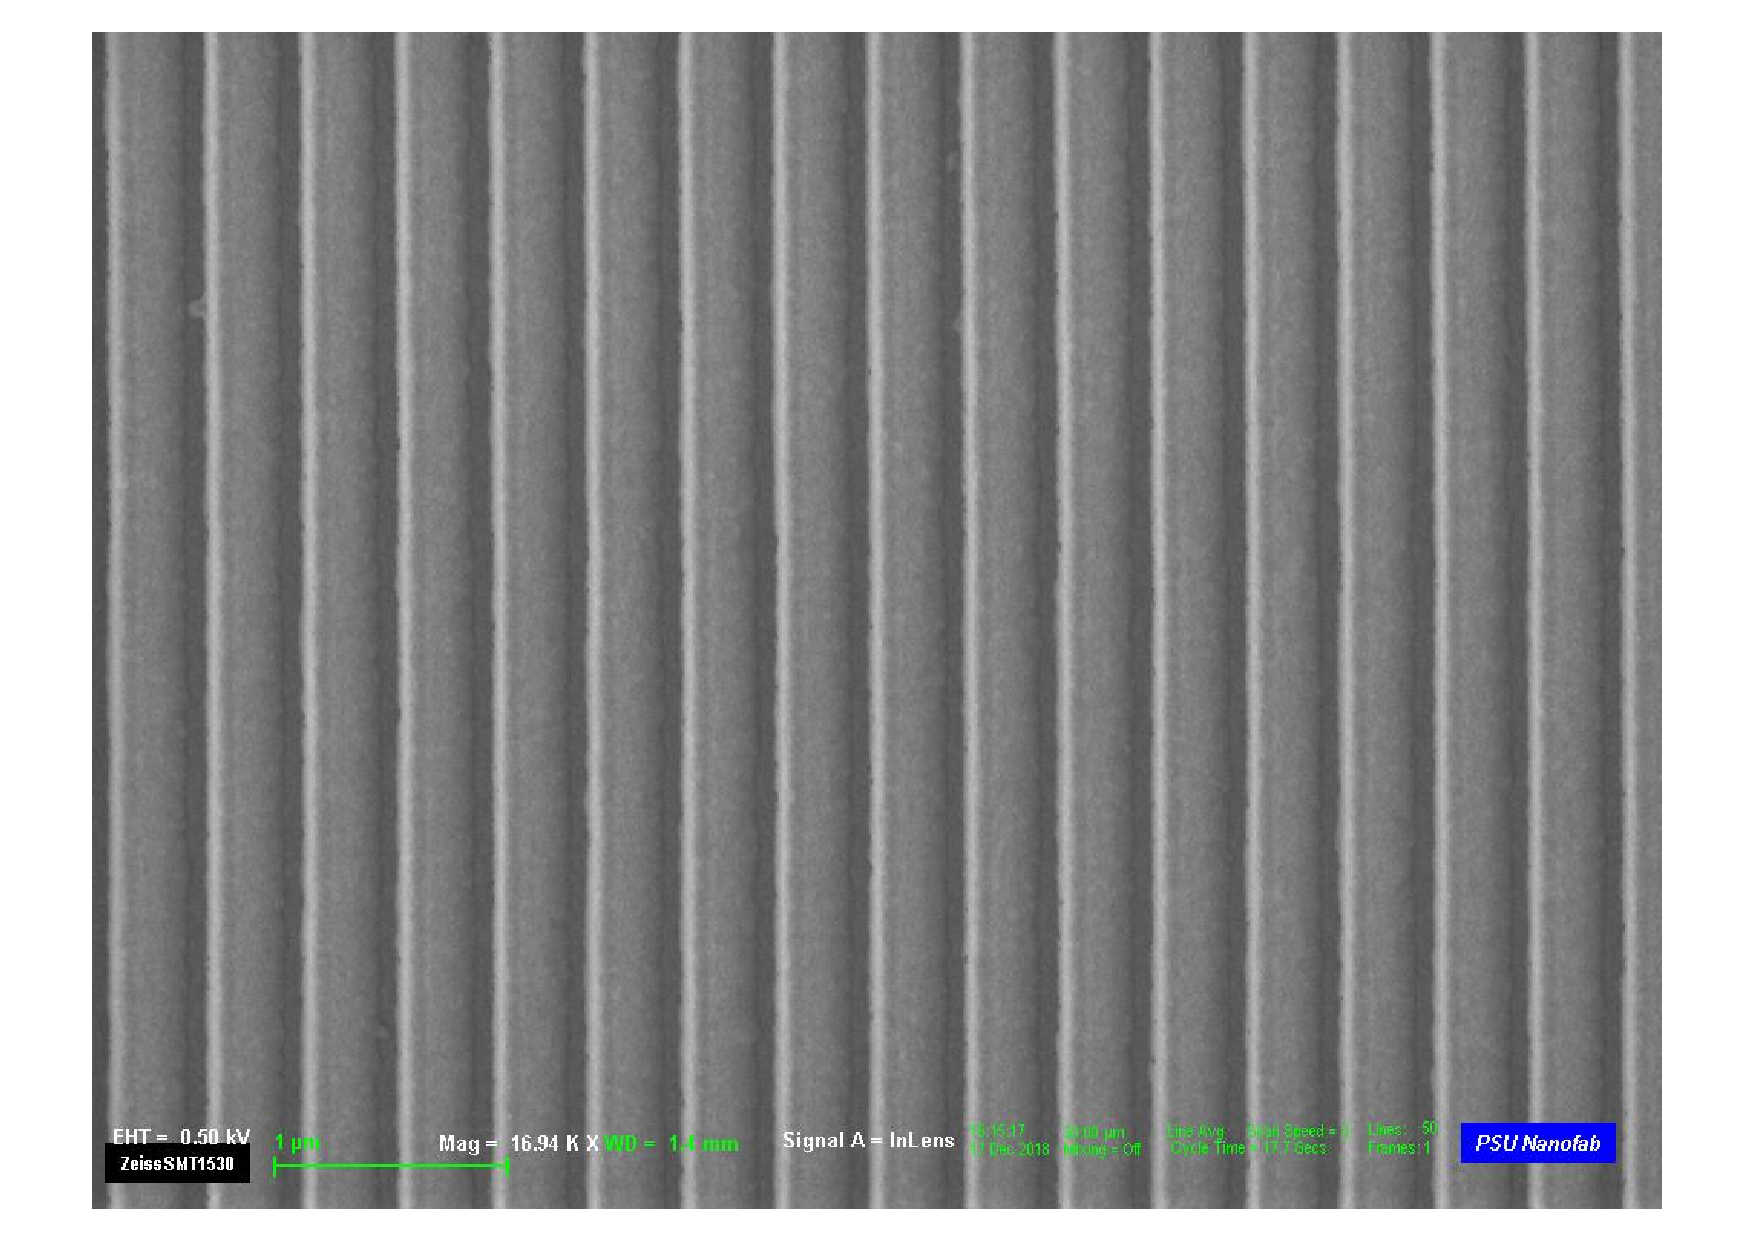
\includegraphics[scale=0.205]{Figures/coated_SEM.pdf}
 \vspace{-5mm}
 \caption{FESEM of gold-coated grooves}\label{fig:coating_SEM}
 \end{figure}
  \vspace{-5mm}
 \begin{block}{\footnotesize \emph{Coating for reflectivity}}
 \centering
  Use \emph{electron-beam physical vapor deposition (EBPVD)} to provide \SI{15}{\nm} \ce{Au} for \emph{thick slab}, \SI{5}{\nm} \ce{Ti} for adhesion
 \end{block}
  \vspace{-1mm}
  \centering {\footnotesize McCoy, et al. (2020a)}
 \end{minipage}
\end{frame}

\subsection{Beamline Experiments}

\begin{frame}{Grating Fabrication by TASTE}
\begin{minipage}[t]{0.45\linewidth}
\vspace{-2mm}
\begin{figure}
 \centering
 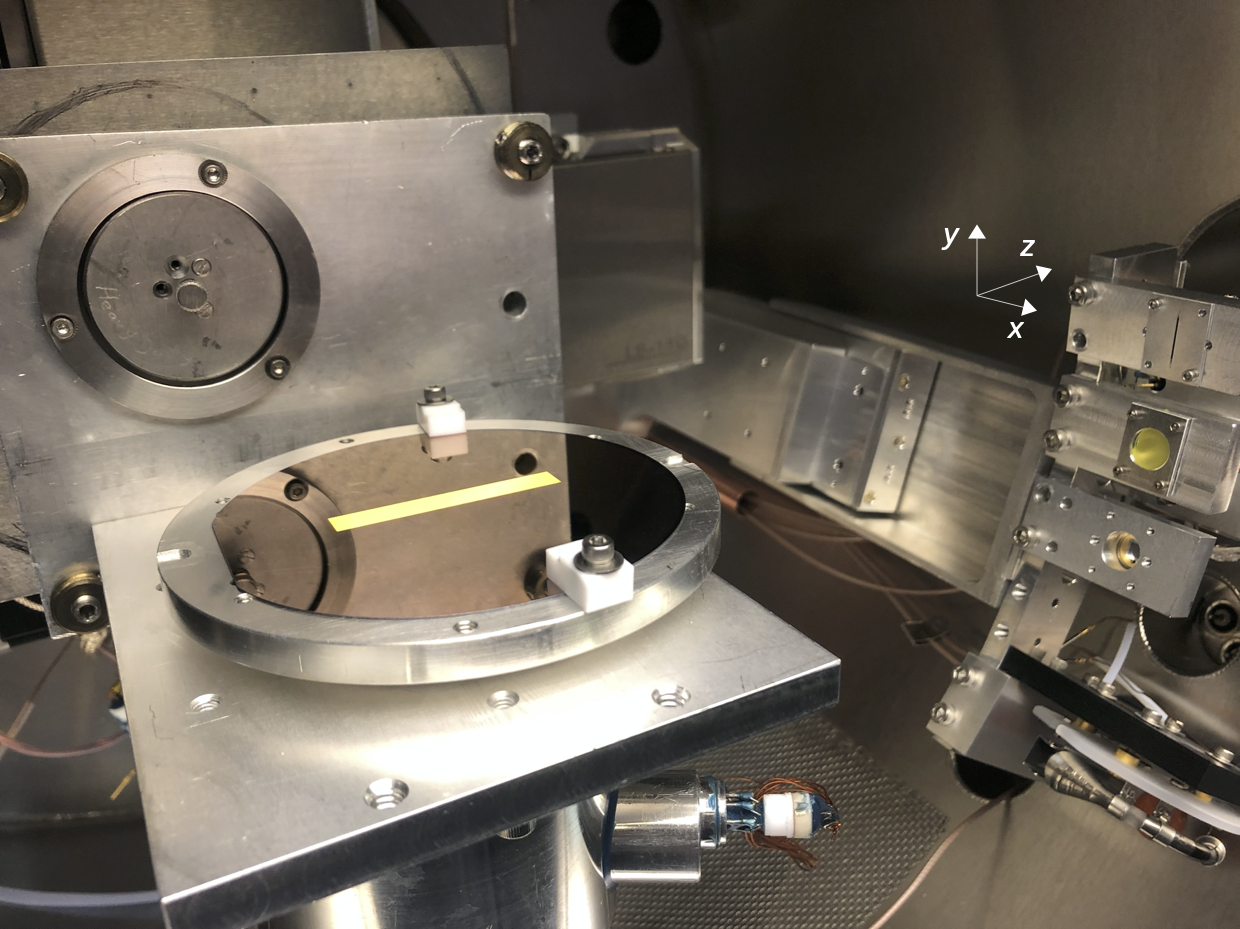
\includegraphics[scale=0.3]{Figures/test_chamber_edit.png}
 \caption{Grating prototype installed inside test chamber of ALS beamline 6.3.2}
 \end{figure} 
 \vspace{-4mm}
 \begin{itemize}
  \item Establish near-Littrow configuration
  \item Measure $\mathscr{E}_n$ across soft x-ray range with separable orders, into EUV
 \end{itemize}
 \end{minipage}
 %\hspace{1mm}
 \begin{minipage}[t]{0.54\linewidth}
 \vspace{-3mm}
 \begin{figure}
  \centering
  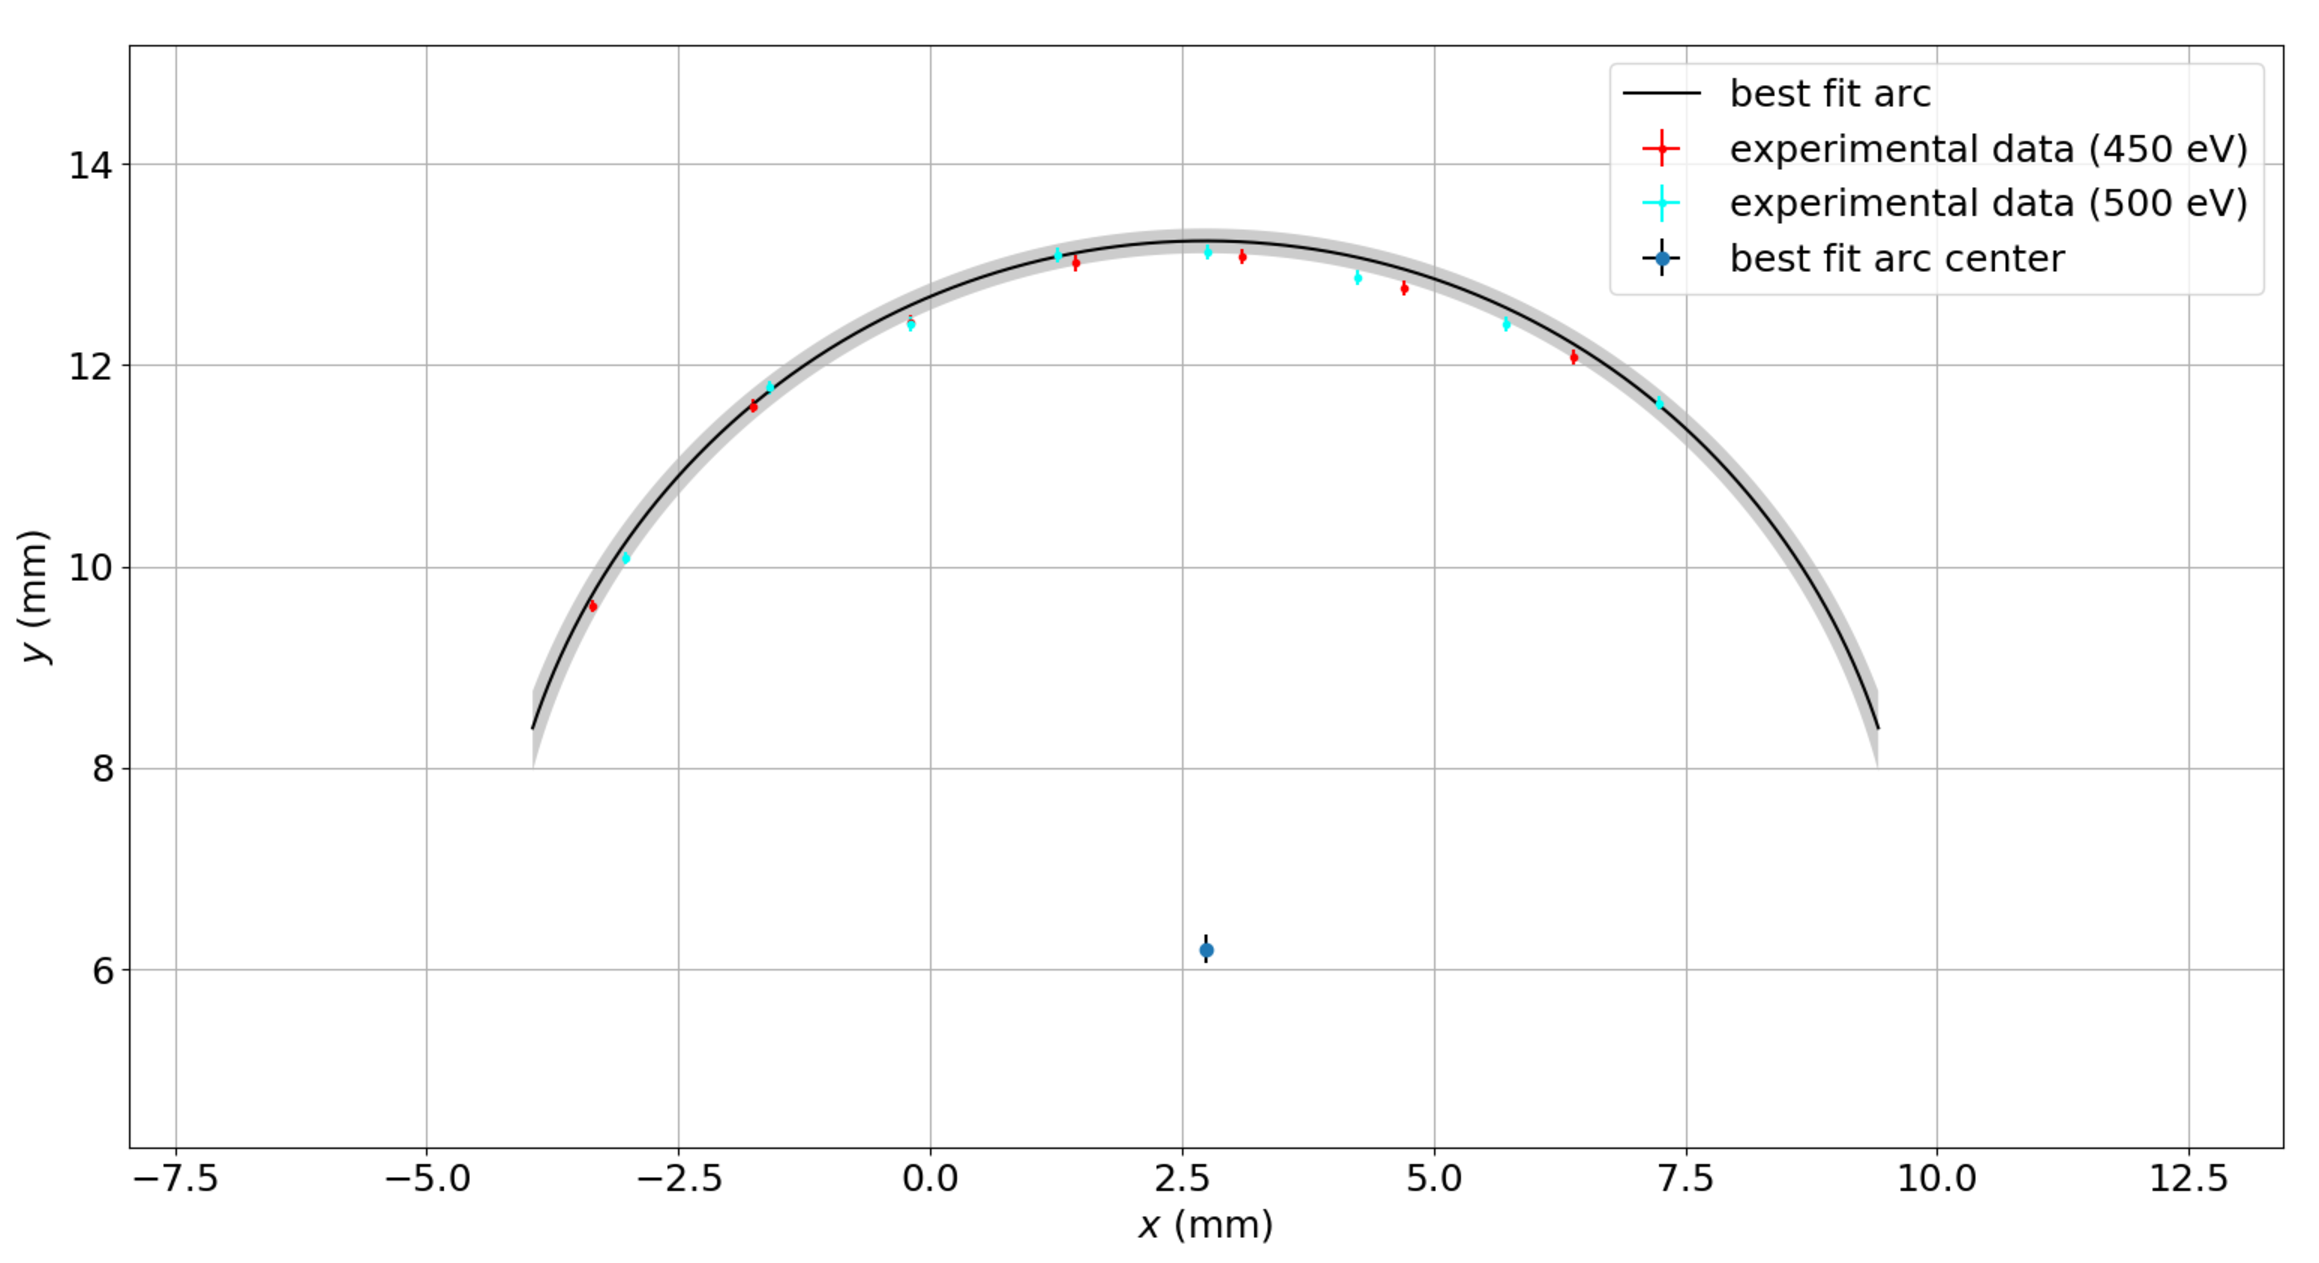
\includegraphics[scale=0.2]{Figures/arc_fit.pdf}
  \caption{Test-configuration diffracted arc mapped using \SI{450}{\electronvolt} and \SI{500}{\electronvolt} data fit to circle}%{Test-configuration diffracted arc mapped using data gathered at \SI{450}{\electronvolt} and \SI{500}{\electronvolt} and fit to a circle. Grayed regions represent one standard deviation uncertainty.}\label{fig:arc_fit_taste}
 \end{figure}
 \vspace{-3mm}
 \begin{table}[]
\centering \footnotesize
\begin{tabular}{@{}ll@{}}
\toprule
parameter                                                                 & measured value             \\ \midrule
system throw ($L$)                                                        & $232.0 \pm 1.4$ mm     \\
arc radius ($r$)                                                          & $7.03 \pm 0.12$ mm       \\
%$x$-distance between direct beam and arc center ($\Delta x_{\text{dir}}$) & $2.80 \pm 0.05$ mm       \\
%$x$-distance between 0$^{\text{th}}$ order and arc center ($\Delta x_0$)  & $2.92 \pm 0.05$ mm       \\
%$y$-distance between 0$^{\text{th}}$ order and arc center ($\Delta y_0$)  & $6.33 \pm 0.14$ mm       \\ \midrule
cone opening half-angle ($\gamma$)                                        & $1.73 \pm 0.03^{\circ}$  \\
azimuthal incidence angle ($\alpha$)                                      & $23.4 \pm 0.6^{\circ}$ \\ \bottomrule %\midrule
%roll (rotation about $z$-axis; $\phi$)                                    & $1.14 \pm 0.04^{\circ}$  \\
%graze (rotation about $x$-axis; $\eta$)                                   & $1.56 \pm 0.04^{\circ}$  \\
%yaw (rotation about $y$-axis; $\varphi$)                                  & $0.69 \pm 0.01^{\circ}$  \\ \bottomrule
\end{tabular}
%\caption{Measured parameters for test-configuration diffracted arc}\label{tab:arc_params_taste}
\end{table}
 \end{minipage}
\end{frame}

\subsection{Analysis \& Discussion for Diffraction Efficiency}

\begin{frame}{Grating Fabrication by TASTE}
\begin{minipage}[t]{0.66\linewidth}
\vspace{-2mm}
\begin{figure}
 \centering
 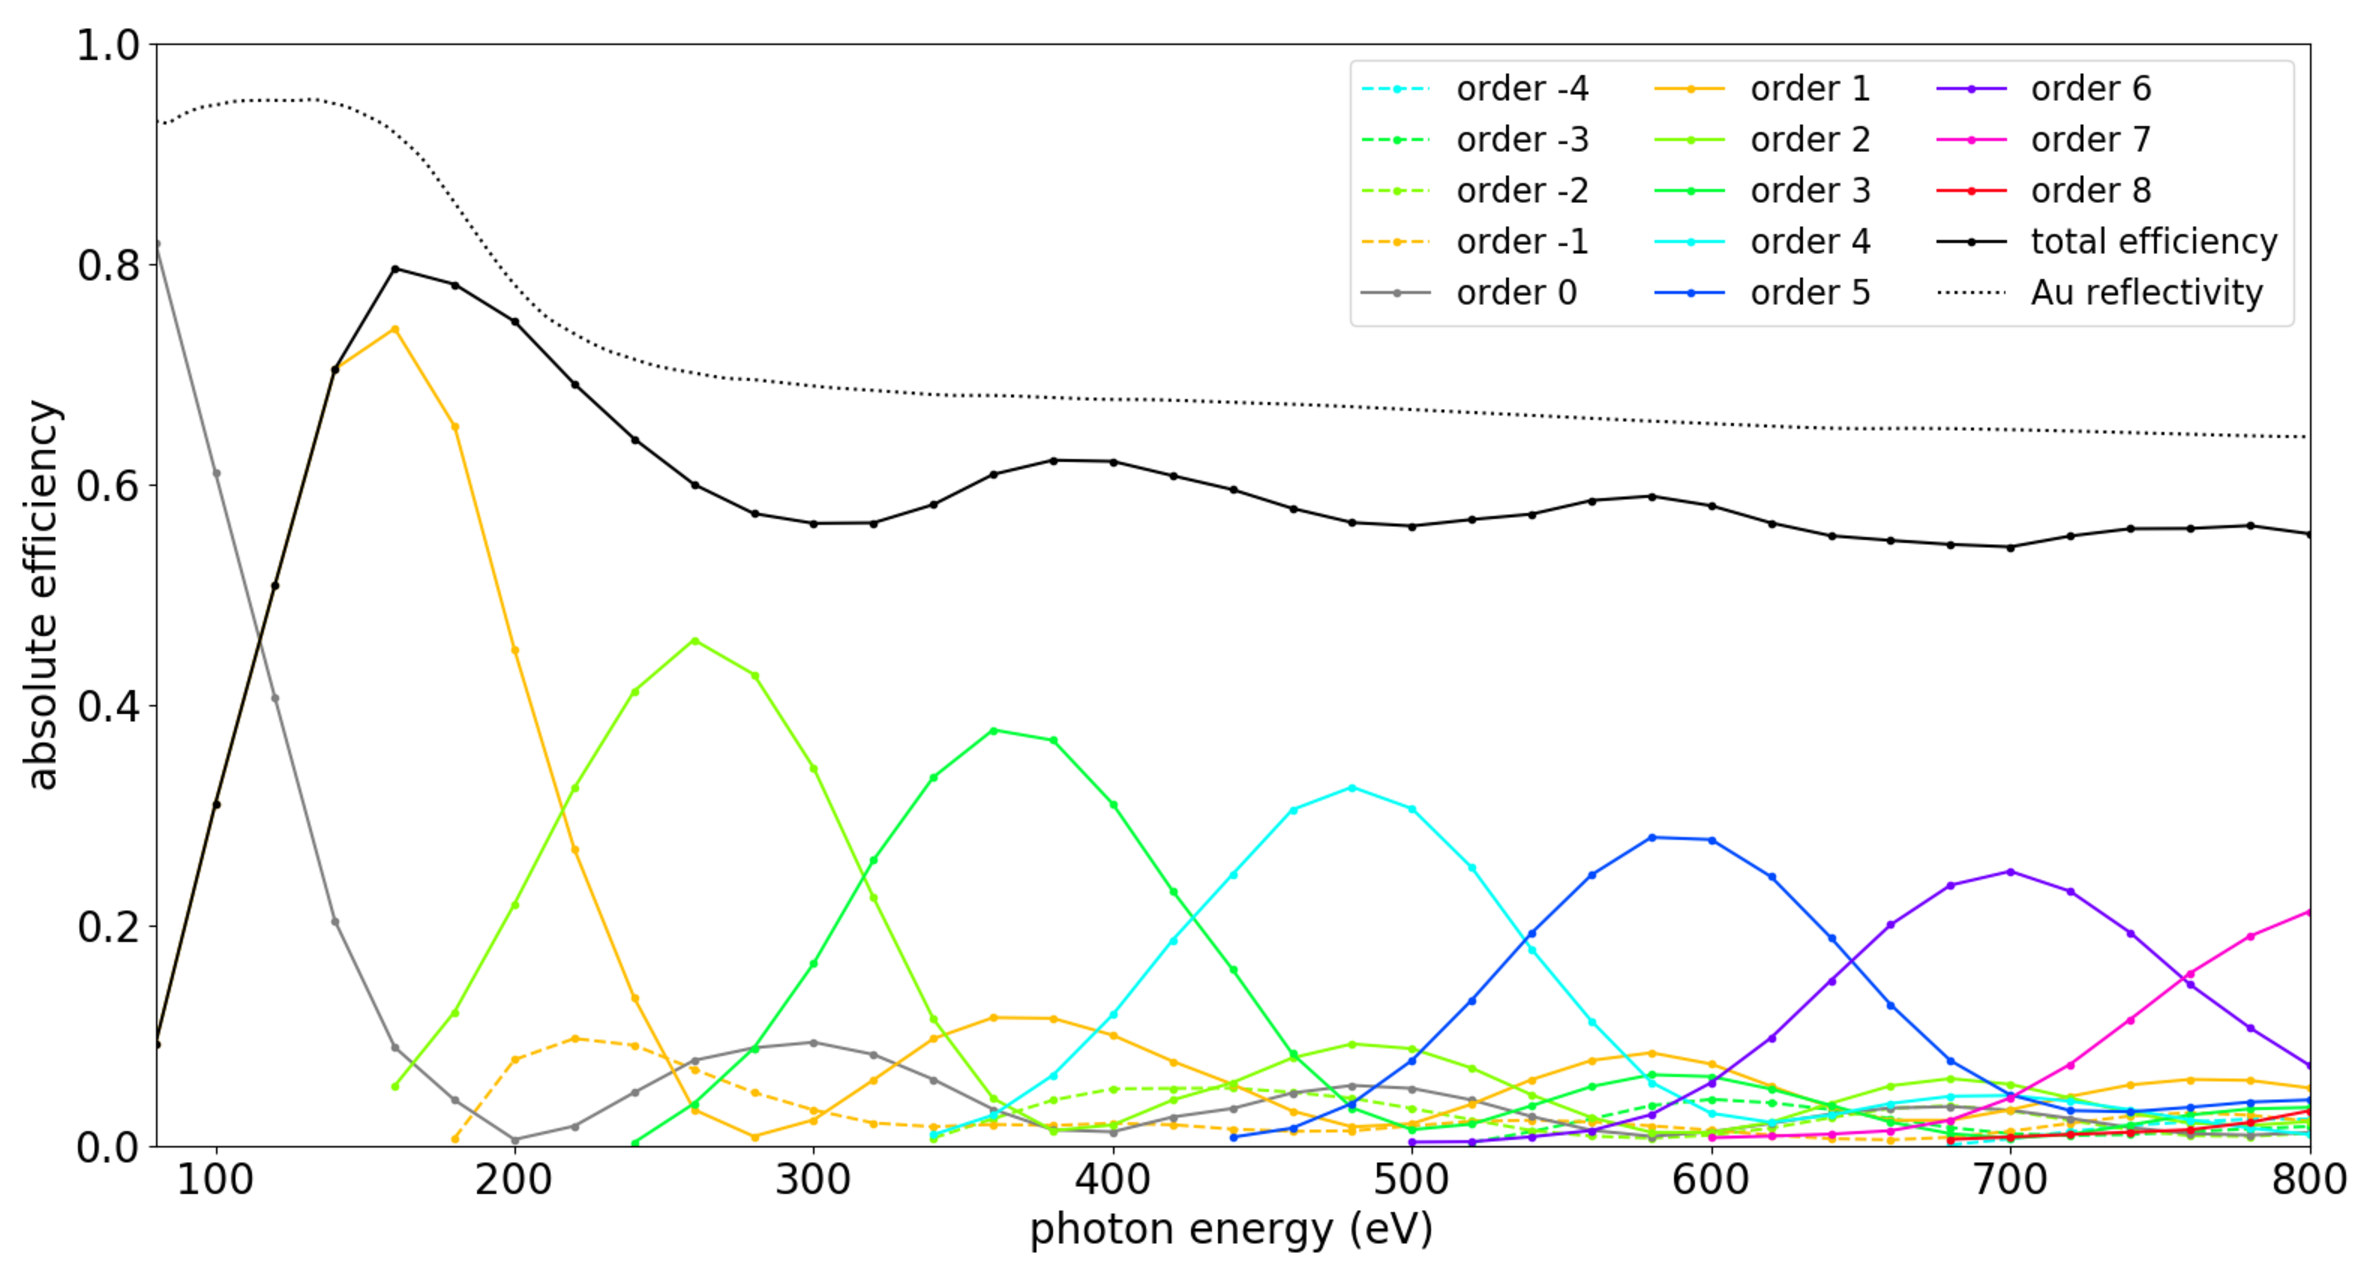
\includegraphics[scale=0.25]{Figures/absolute_efficiency_data.pdf}
 \caption{Measured absolute $\mathscr{E}_n$ for prototype compared to $\mathcal{R}_F$ of gold}%{Absolute diffraction efficiency data gathered at the ALS compared to the Fresnel reflectivity of gold, $\mathcal{R}_{F}$. Total diffraction efficiency below \SI{240}{\electronvolt} misses contributions from orders $n = \num{2}$ and $n = \num{3}$ on the order of a few percent.}\label{fig:abs_eff_taste}
 \end{figure} 
 \vspace{-3mm}
 \centering {$\mathscr{E}_{\text{tot}} \equiv \sum_n \mathscr{E}_n \ \ \text{for} \ \ n \neq 0$ $\implies$ exceeds \SI{40}{\percent}}
 \end{minipage}
 \begin{minipage}[t]{0.33\linewidth}
 \textbf{Measuring efficiency}
 \begin{itemize}
  \item $\mathscr{E}_n = \mathcal{I}_n / \mathcal{I}_{\text{inc}}$ with dark current, diffuse scatter subtracted
  \begin{itemize}
    \item[$\square$] Measure in \SI{20}{\electronvolt} steps
  \end{itemize}
  %\item Diffuse scatter: level of $\lessapprox \SI{1}{\percent}$ for $\mathcal{E}_{\gamma} \gtrapprox \SI{600}{\electronvolt}$
  %\item Measurements taken in \SI{20}{\electronvolt} steps: \SIrange{440}{800}{\electronvolt} and then \SIrange{80}{420}{\electronvolt} with order sorter
  \item Peak-order $\mathscr{E}_n$ ranges from \SIrange{75}{25}{\percent} as $\mathcal{E}_{\gamma}$ increases
  \begin{itemize}
    \item[$\square$] Diffracted orders become suppressed with increasing $n$ %$\mathscr{E}_{\text{tot}}$ dominated by single orders but lower $n$ contribute to $\mathscr{E}_{\text{tot}}$ at level of $\sim \SI{10}{\percent}$
    \item[$\implies$] Likely due to imperfect sawtooth topography generated by TASTE 
  \end{itemize}
  \item Total efficiency in soft x-ray meets \emph{Lynx} requirements
    \begin{itemize}
    \item[$\square$] $\mathscr{E}_{\text{tot}} \approx \SI{60}{\percent}$
    \item[$\square$] $\mathscr{E}_{\text{tot}} / \mathcal{R}_{F} \lessapprox \SI{95}{\percent}$  %ranges from \SIrange{95}{88}{\percent} as $\mathcal{E}_{\gamma}$ increases from \SIrange{240}{800}{\electronvolt}
    %\item[$\square$] Missing orders: $\mathcal{E}_{\gamma} < \SI{240}{\electronvolt}$
  \end{itemize}
  %\item Diffracted orders become suppressed with increasing $n$ 
  %\begin{itemize}
   %   \item[$\square$] $\mathscr{E}_{\text{tot}}$ dominated by single orders but lower $n$ contribute to $\mathscr{E}_{\text{tot}}$ at level of $\sim \SI{10}{\percent}$
   % \item[$\square$] Likely due to imperfect sawtooth topography generated by TASTE 
  %\end{itemize}
 \end{itemize}
 \vspace{5mm}
 \centering {\footnotesize McCoy, et al.~(2020a)}
 \end{minipage}
\end{frame}

\begin{frame}{Grating Fabrication by TASTE}
\begin{minipage}[t]{0.66\linewidth}
\vspace{-2mm}
\begin{figure}
 \centering
 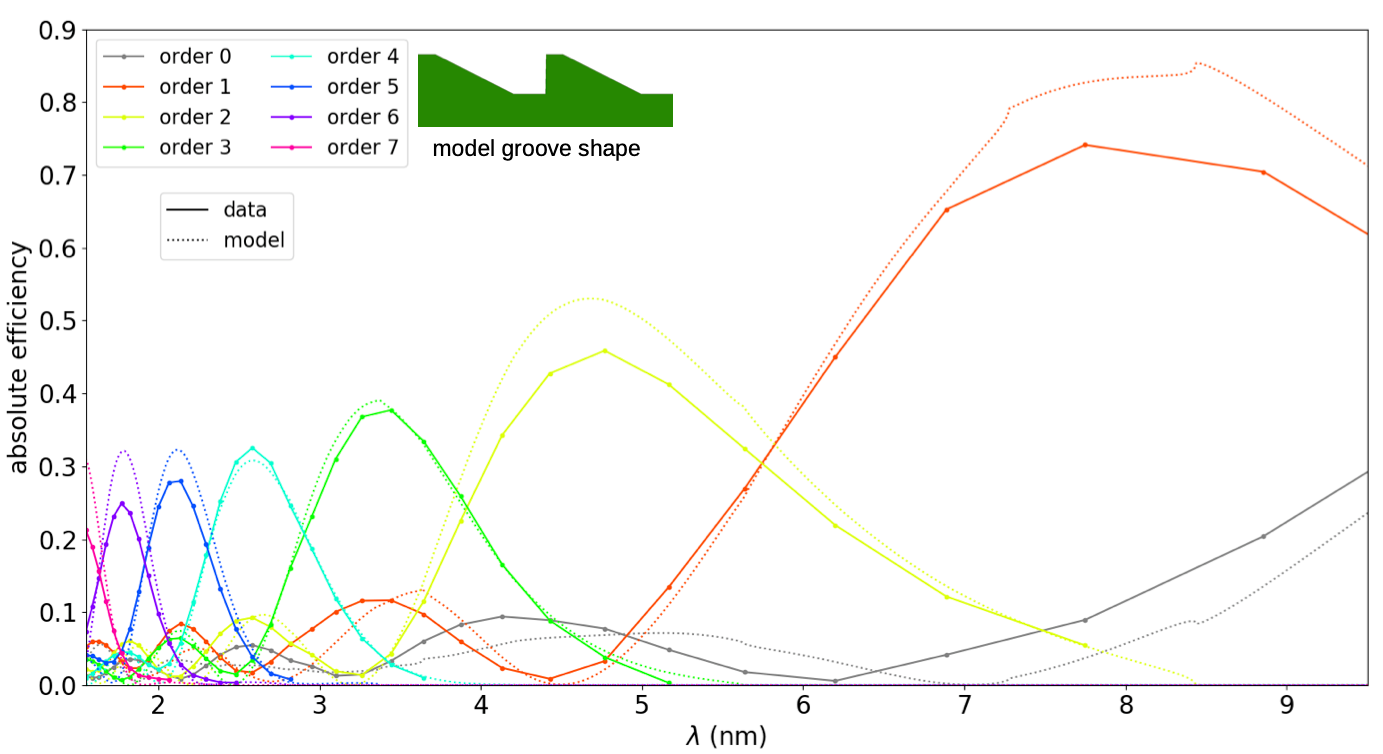
\includegraphics[scale=0.41]{Figures/absolute_efficiency_model_wav.pdf} %85 nm land, 120 nm depth, 77 nm ridge, 27 blaze angle, 89 steep angle
 \caption{Measured $\mathscr{E}_n$ compared to theoretical $\mathscr{E}_n$ modeled using \textsc{PCGrate-SX}}%{Absolute diffraction efficiency from \cref{fig:abs_eff_taste} compared to theoretical diffraction efficiency modeled using \textsc{PCGrate-SX}. Modeled data are multiplied by the Nevot-Croce factor [\emph{cf.\@} \cref{eq:nc_factor_taste}] for $\zeta = 1.73^{\circ}$ and $\sigma = \SI{1.5}{\nm}$ RMS.}\label{fig:model_eff_taste}
 \end{figure}
  %\centering{$\implies$ \footnotesize Facet roughness taken into account with NC factor}
 \end{minipage}
\begin{minipage}[t]{0.33\linewidth}
 \textbf{Efficiency modeling}
 \begin{itemize}
  \item Investigate impact of unpointed apex on measured $\mathscr{E}_n$
  \item Approximate groove shape as acute trapezoid with $\delta \approx 27^{\circ}$%with near-vertical lateral side and slope that emulates active blaze facet with $\delta \approx 27^{\circ}$
  \begin{itemize}
    \item[$\square$] Include flat bottom to represent cleared portion%of resist
  \end{itemize}
  \item Keep $\gamma = 1.73^{\circ}$, $\alpha = 23.4^{\circ}$ and $d = \SI{400}{\nm}$ fixed, vary model
  \item Amplitudes of peak orders generally fall short of model
  \item Deviations from ideal acute trapezoid expected to have impact on $\mathscr{E}_n$ distribution among orders
 \end{itemize}
  \vspace{3mm}
 \centering {\footnotesize McCoy, et al.~(2020a)}
 \end{minipage}
\end{frame}


\section{Grating Replication by Substrate-Conformal Imprint Lithography (SCIL)} %for Replication of X-ray Reflection Gratings

\begin{frame}{Grating Replication by SCIL}
 \begin{minipage}[t]{0.47\linewidth}
 \textbf{Substrate-Conformal Imprint Lithography (SCIL)}
 \begin{itemize}
  \item \textsc{Philips SCIL Nanoimprint Solutions} in Eindhoven, Netherlands
  \item Form flexible, composite stamp from rigid master template
  \item Use stamp (rather than master) to produce replicas in various resists
 \end{itemize}
  \textbf{Alternative to UV-NIL}
 \begin{itemize}
  \item Stamp features carried in modified PDMS %\footnote{polydimethylsiloxane} %with increased Young’s modulus
  \item Conforms locally to particulate contaminants, globally to bow of replica substrate %, while avoiding damage to master template by eliminating high pressure
  \item Wave-like sequential imprinting serves to eliminate large trapped air pockets
  %\item \emph{Cue video}
  %\item Packaged equipment automates spin-coating, wafer-scale imprint method for high-volume replication (\textsc{AutoSCIL})
  %\item grating spectrometer on board the \emph{Water Recovery X-ray Rocket}: 26 nickel-coated replicas of \SI{110}{\cm\squared} master grating fabricated through crystallographic etching
 \end{itemize}
 \end{minipage}
\hspace{1mm}
\begin{minipage}[t]{0.51\linewidth}
\begin{figure}
 \centering
 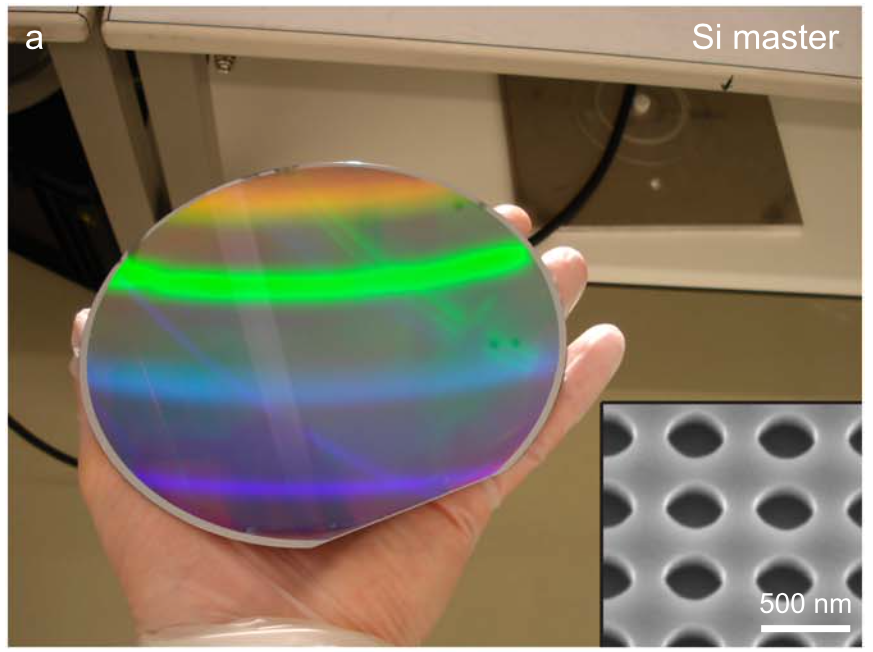
\includegraphics[scale=0.25]{Figures/scil_A.png}
 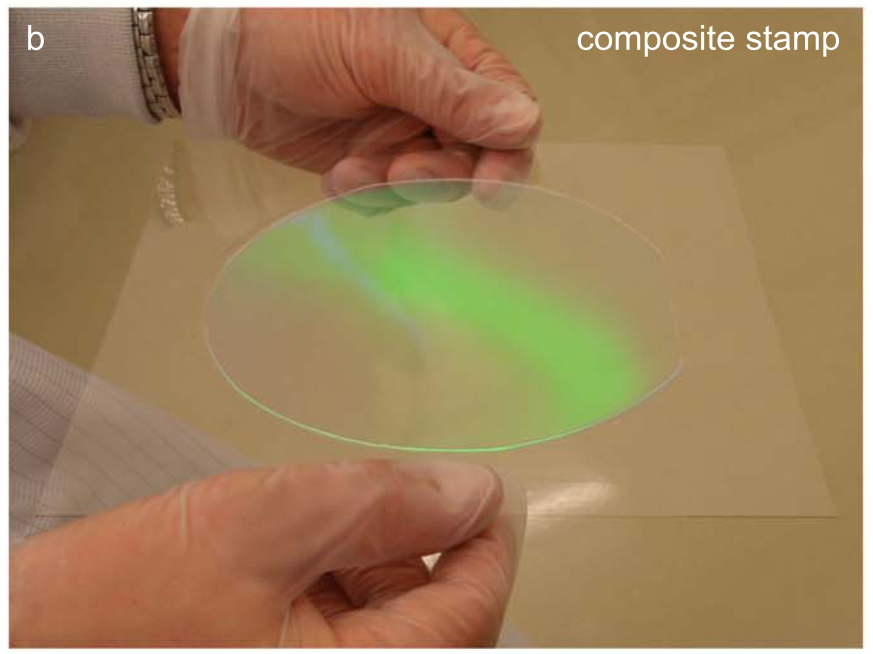
\includegraphics[scale=0.25]{Figures/scil_B.png}
 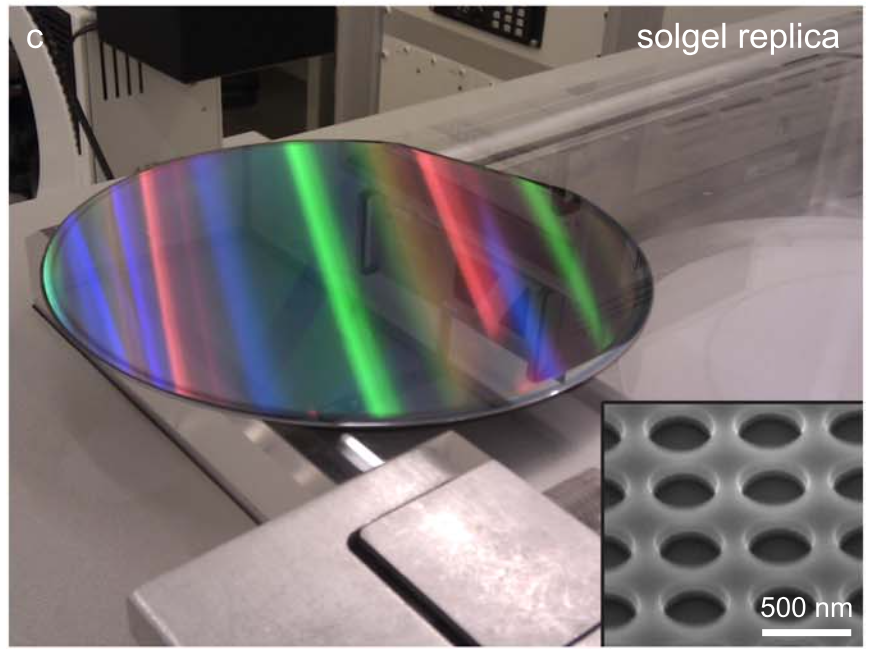
\includegraphics[scale=0.25]{Figures/scil_C.png}
 \caption{Overview of SCIL: a) master template, b) composite stamp, c) imprint in resist (Verschuuren, et al.~2019)}
 \end{figure}
 \end{minipage}
\end{frame}

\begin{frame}{Grating Replication by SCIL}
 \begin{minipage}[t]{0.55\linewidth}
 \textbf{\textsc{NanoGlass} sol-gel resist}
 \begin{itemize}
  \item High-volume production relies on long stamp lifetime
  \begin{itemize}
    \item[$\square$] Best suited for inorganic resist that cures through silica \emph{sol-gel} process (\textsc{NanoGlass})
    %\item[$\square$] Precursors in water/alcohol react to form gel, solid silica-like network as $T$ increases
  \end{itemize}
  \item Single stamp produces $\gtrapprox \num{700}$ imprints in \textsc{NanoGlass} %resist %(60 wafers per hour, over \SI{150}{\mm})
  \begin{itemize}
    \item[$\square$] 60 wafers per hour, over \SI{150}{\mm}
    \item[$\square$] Beneficial for \emph{Lynx XGS}, sounding rockets
  \end{itemize}
  \item \textsc{AutoSCIL}, \textsc{NanoGlass} used for \emph{WRXR}% grating spectrometer on board \emph{WRXR}%\emph{Water Recovery X-ray Rocket}
  \begin{itemize}
    \item[$\square$] 26 replicas of \SI{110}{\cm\squared} master grating %fabricated through crystallographic etching
    %\item[$\square$] Beneficial for \emph{tREXS}, \emph{OGRE}, \emph{Lynx XGS}
  \end{itemize}
  \item Resist shrinkage $\implies$ topographic distortion
  \begin{itemize}
    \item[$\square$] Imprinted resist initially has $\sim \SI{70}{\percent}$ density of fused silica
    %\item[$\square$] Densify for stability through bake at $T_{\text{cure}} \gtrapprox \SI{50}{\celsius}$ %to induce further cross-linking  %in network
    \item[$\square$] $\sim \SI{10}{\percent}$ volume shrinkage expected for $T_{\text{cure}} \approx \SI{90}{\celsius}$
  \end{itemize}
 \end{itemize}
 \vspace{2mm}
 \centering{$\implies$ Study impact of resist shrinkage on blaze angle}
 \end{minipage}
\hspace{1mm}
\begin{minipage}[t]{0.42\linewidth}
\vspace{-3mm}
\begin{figure}
 \centering
 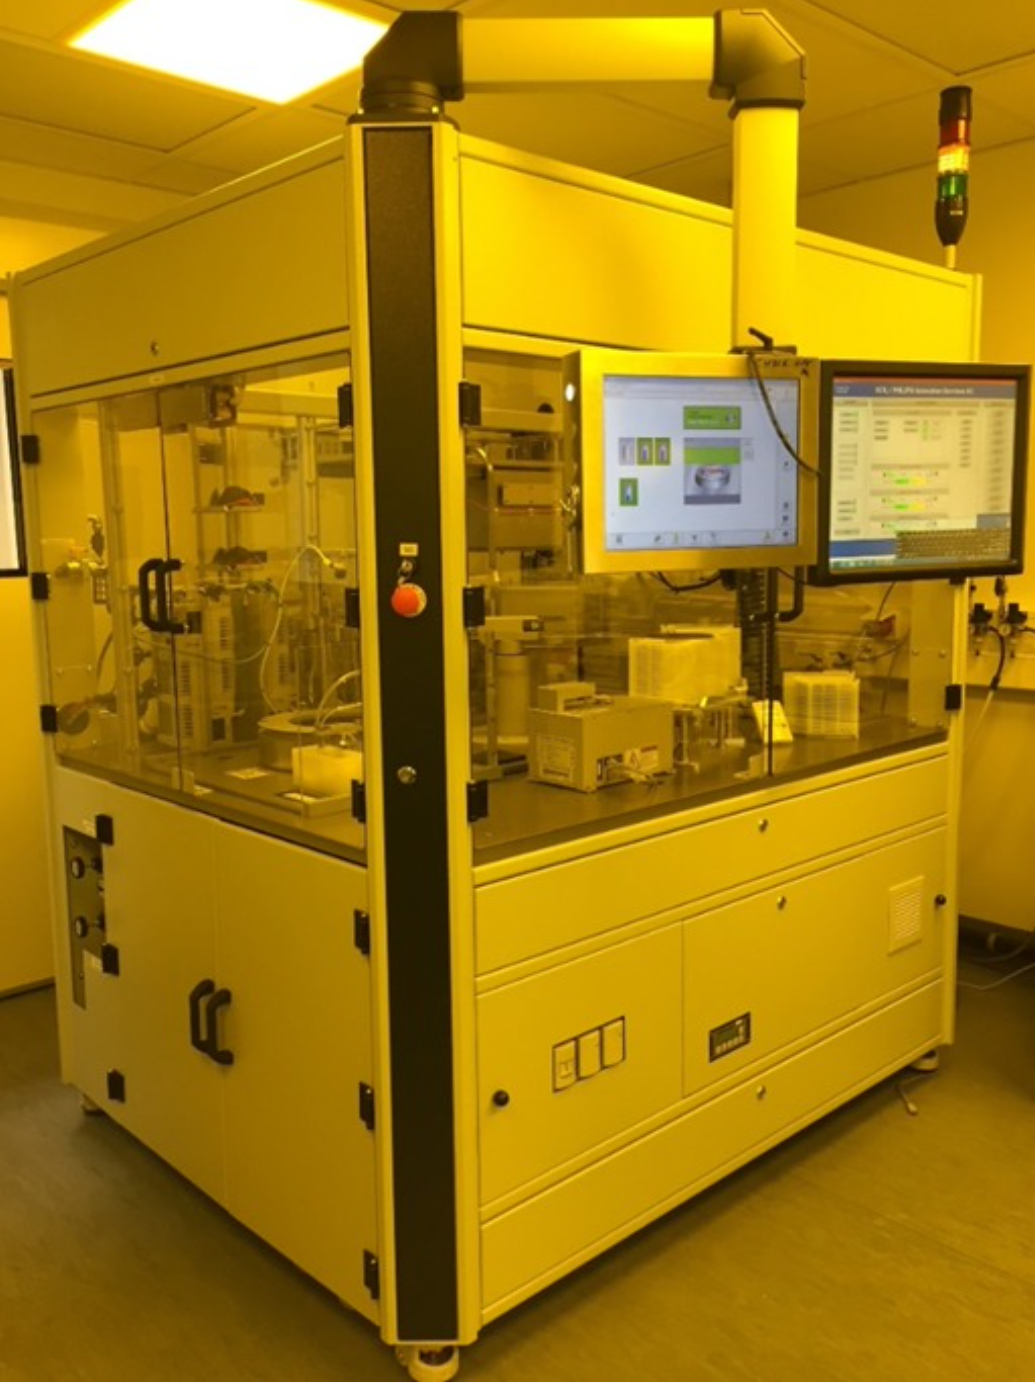
\includegraphics[scale=0.27]{Figures/autoscil.png}
 \vspace{-2mm}
 \caption{\textsc{AutoSCIL} tool (Verschuuren, et al.~2018)}
 \end{figure}
 \end{minipage}
\end{frame}

\subsection{SCIL Process for X-ray Reflection Gratings}


\begin{frame}{Grating Replication by SCIL}
\begin{minipage}[t]{0.46\linewidth}
\vspace{-1mm}
\begin{figure}
 \centering
 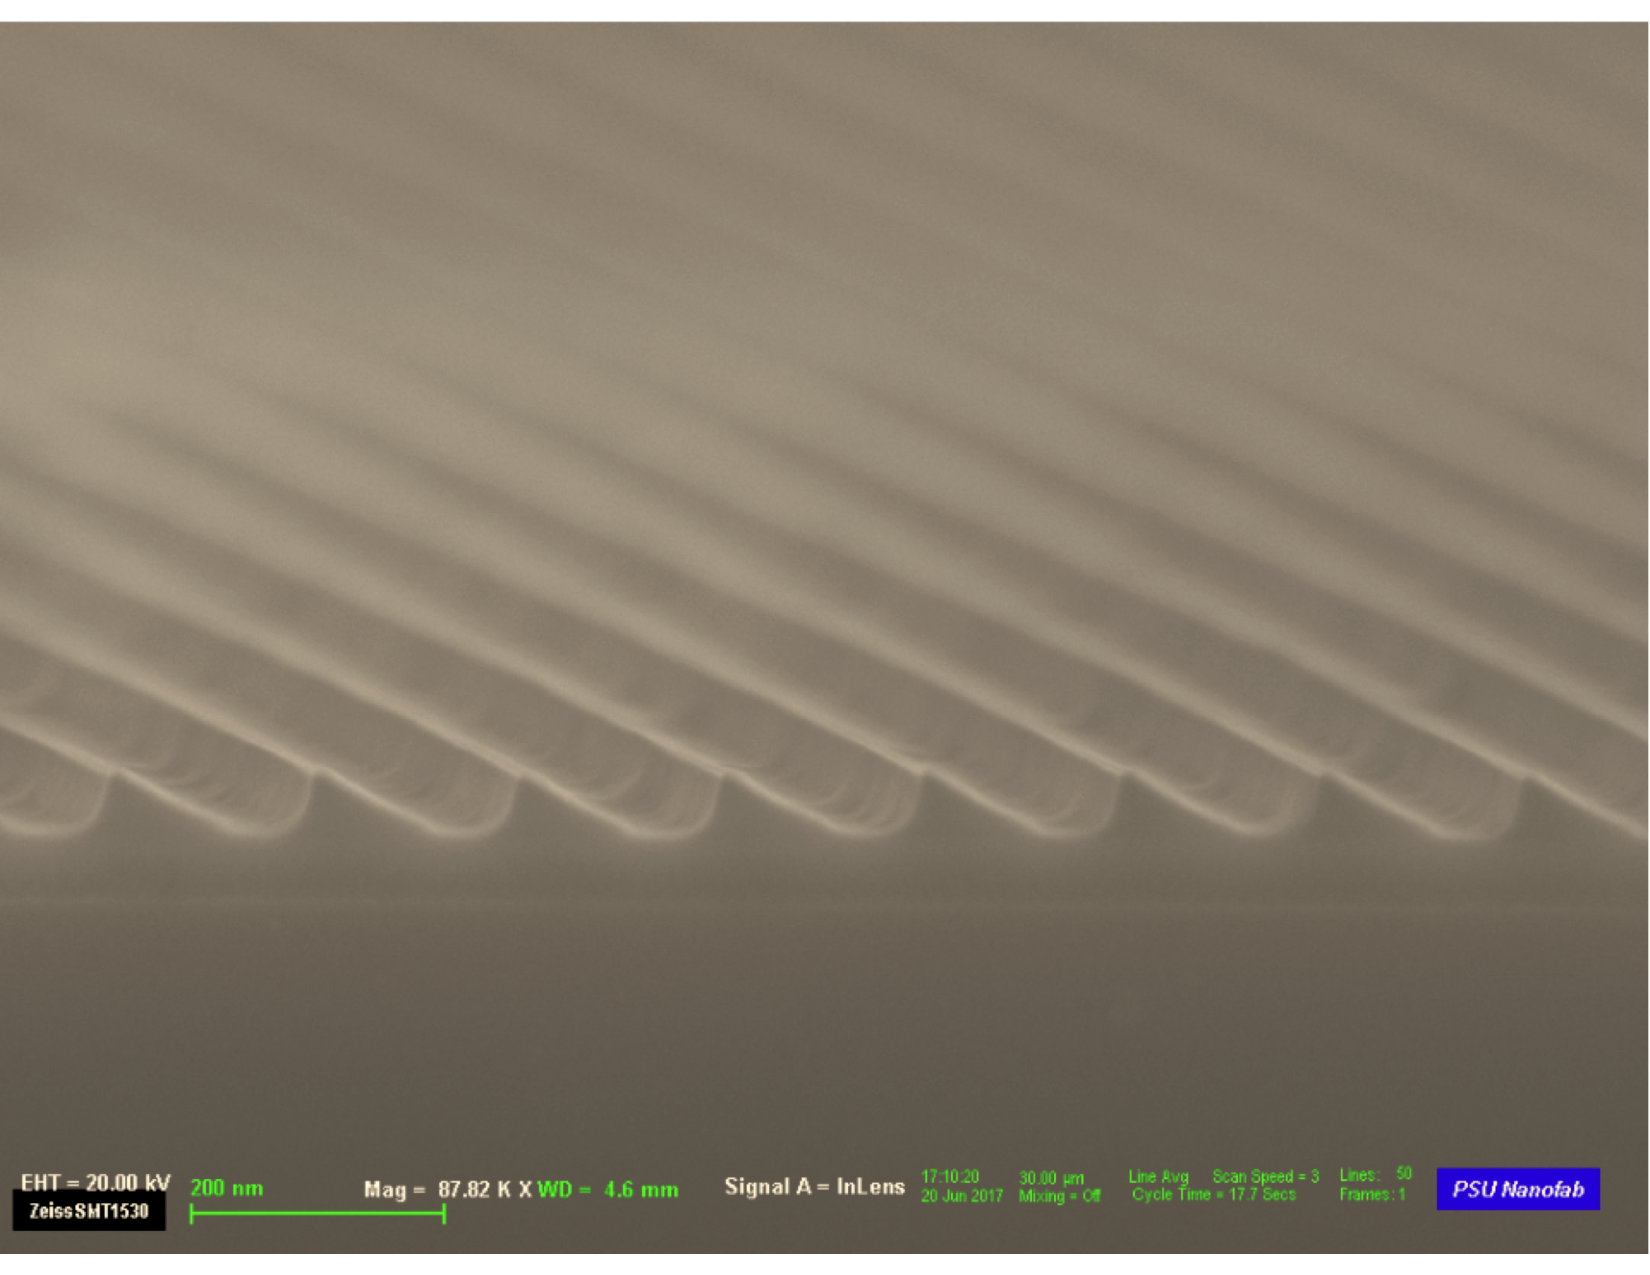
\includegraphics[scale=0.23]{Figures/scil_replica.pdf}
 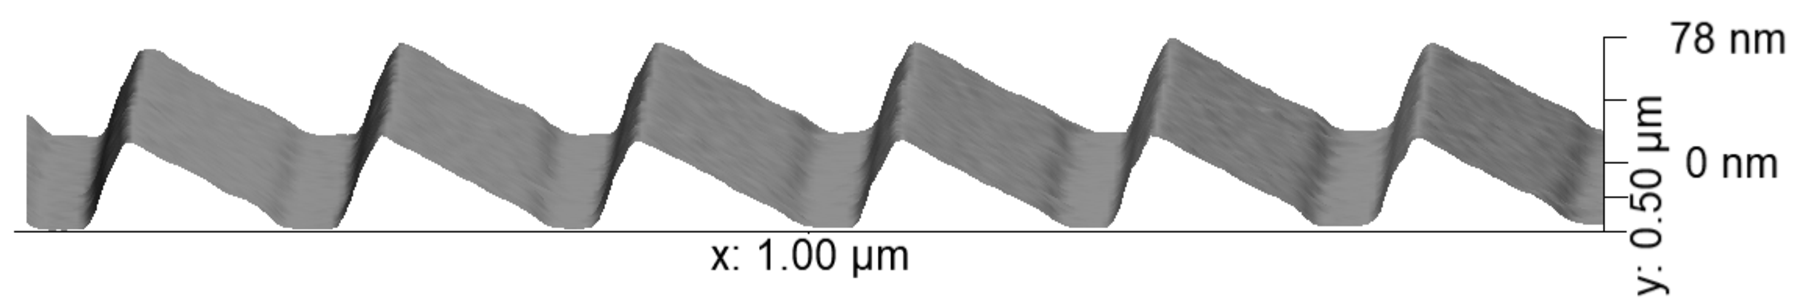
\includegraphics[scale=0.25]{Figures/AFM_bare.pdf}
 \vspace{-6mm}
 \caption{Cross-section FESEM (\emph{top}), AFM (\emph{bottom}) of grating imprint in \textsc{NanoGlass T1100}}%{Cross-section FESEM image of a grating imprint with a groove spacing of $d \lessapprox \SI{160}{\nm}$ in $\sim \SI{100}{\nm}$-thick \textsc{NanoGlass T1100} sol-gel resist coated on a silicon wafer. This topography was produced from an inverted composite stamp [\emph{cf.\@} \cref{fig:scil_stamps}(b)] and then baked to $\SI{90}{\celsius}$ following stamp separation. Image was taken with a \textsc{Zeiss Leo 1530} instrument as in \cref{fig:master_grating_SEM,fig:post_nanostrip}.}\label{fig:SCIL_SEMs} 
 \end{figure} 
%\vspace{-3mm}
% \centering{$\implies$ \SI{10}{\percent} shrinkage hypothesized for $T_{\text{cure}} \approx \SI{90}{\celsius}$}
 \end{minipage}
 \hfill
 \begin{minipage}[t]{0.5\linewidth}
 \vspace{1mm}
  \textbf{SCIL for x-ray reflection gratings}
 \begin{itemize}
  \item Use \ce{KOH}-etched silicon master (Miles, et al.~2018)
  \begin{itemize}
    \item[$\square$] $\delta = 30.0 \pm 0.8^{\circ}$ under AFM
    \item[$\square$] Surface-treat for anti-stiction
  \end{itemize}
  \item Use inverted stamp to produce replicas that emulate UV-NIL gratings using $T_{\text{cure}} \approx \SI{90}{\celsius}$
  \begin{itemize}
    \item[$\square$] $\delta' = 27.9 \pm 0.7^{\circ}$
    \item[$\square$] $\sigma \approx \SI{0.6}{\nm}$ RMS
  \end{itemize}
  \item Sputter-coat with \SI{15}{\nm} of \ce{Au}, using \SI{5}{\nm} \ce{Cr} for adhesion (Miles, et al.~2018)
  \begin{itemize}
    \item[$\square$] $\delta' = 28.4 \pm 0.8^{\circ}$
    \item[$\square$] $\sigma \approx \SI{0.8}{\nm}$ RMS
  \end{itemize}
  %\item Facet roughness measures
 \end{itemize}
 \vspace{-3mm}
 \begin{figure}
 \centering
 \hspace{6mm}
 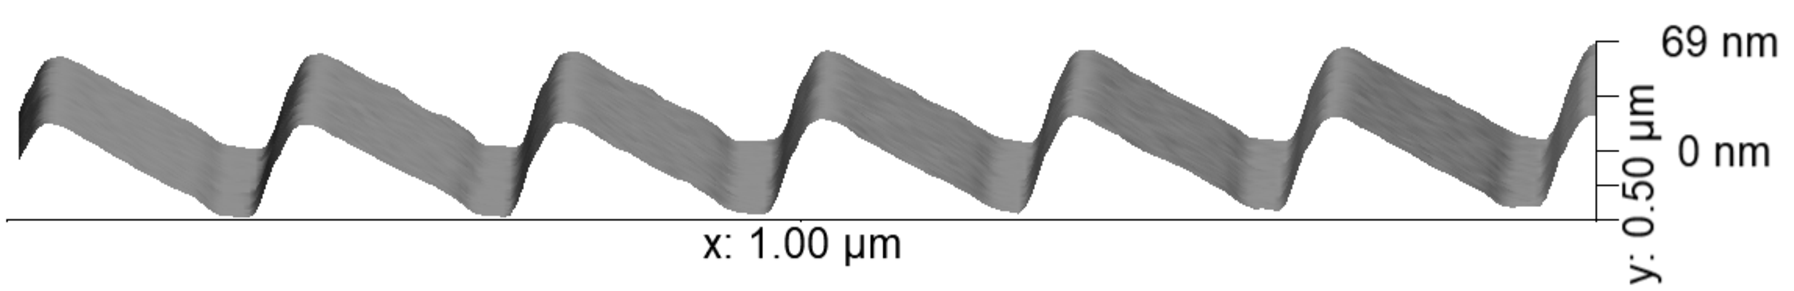
\includegraphics[scale=0.25]{Figures/AFM_coated.pdf}
 \vspace{-2mm}
 \caption{AFM of gold-coated grating imprint}%{AFM image of a grating imprint with a groove spacing of $d \lessapprox \SI{160}{\nm}$ in $\sim \SI{100}{\nm}$-thick \textsc{NanoGlass T1100} sol-gel resist coated on a silicon wafer as in \cref{fig:SCIL_SEMs}. Facet roughness and blaze angle under AFM measure $\sigma \approx \SI{0.6}{\nm}$ RMS and $27.9 \pm 0.7^{\circ}$, respectively.}\label{fig:SCIL_AFMs} 
 \end{figure}
 \vspace{-3mm}
 \centering {\footnotesize McCoy, et al.~(2020b)}
 \end{minipage}
\end{frame}


\subsection{Beamline Experiments}


\begin{frame}{Grating Replication by SCIL}
\begin{minipage}[t]{0.67\linewidth}
\begin{figure}
 \centering
 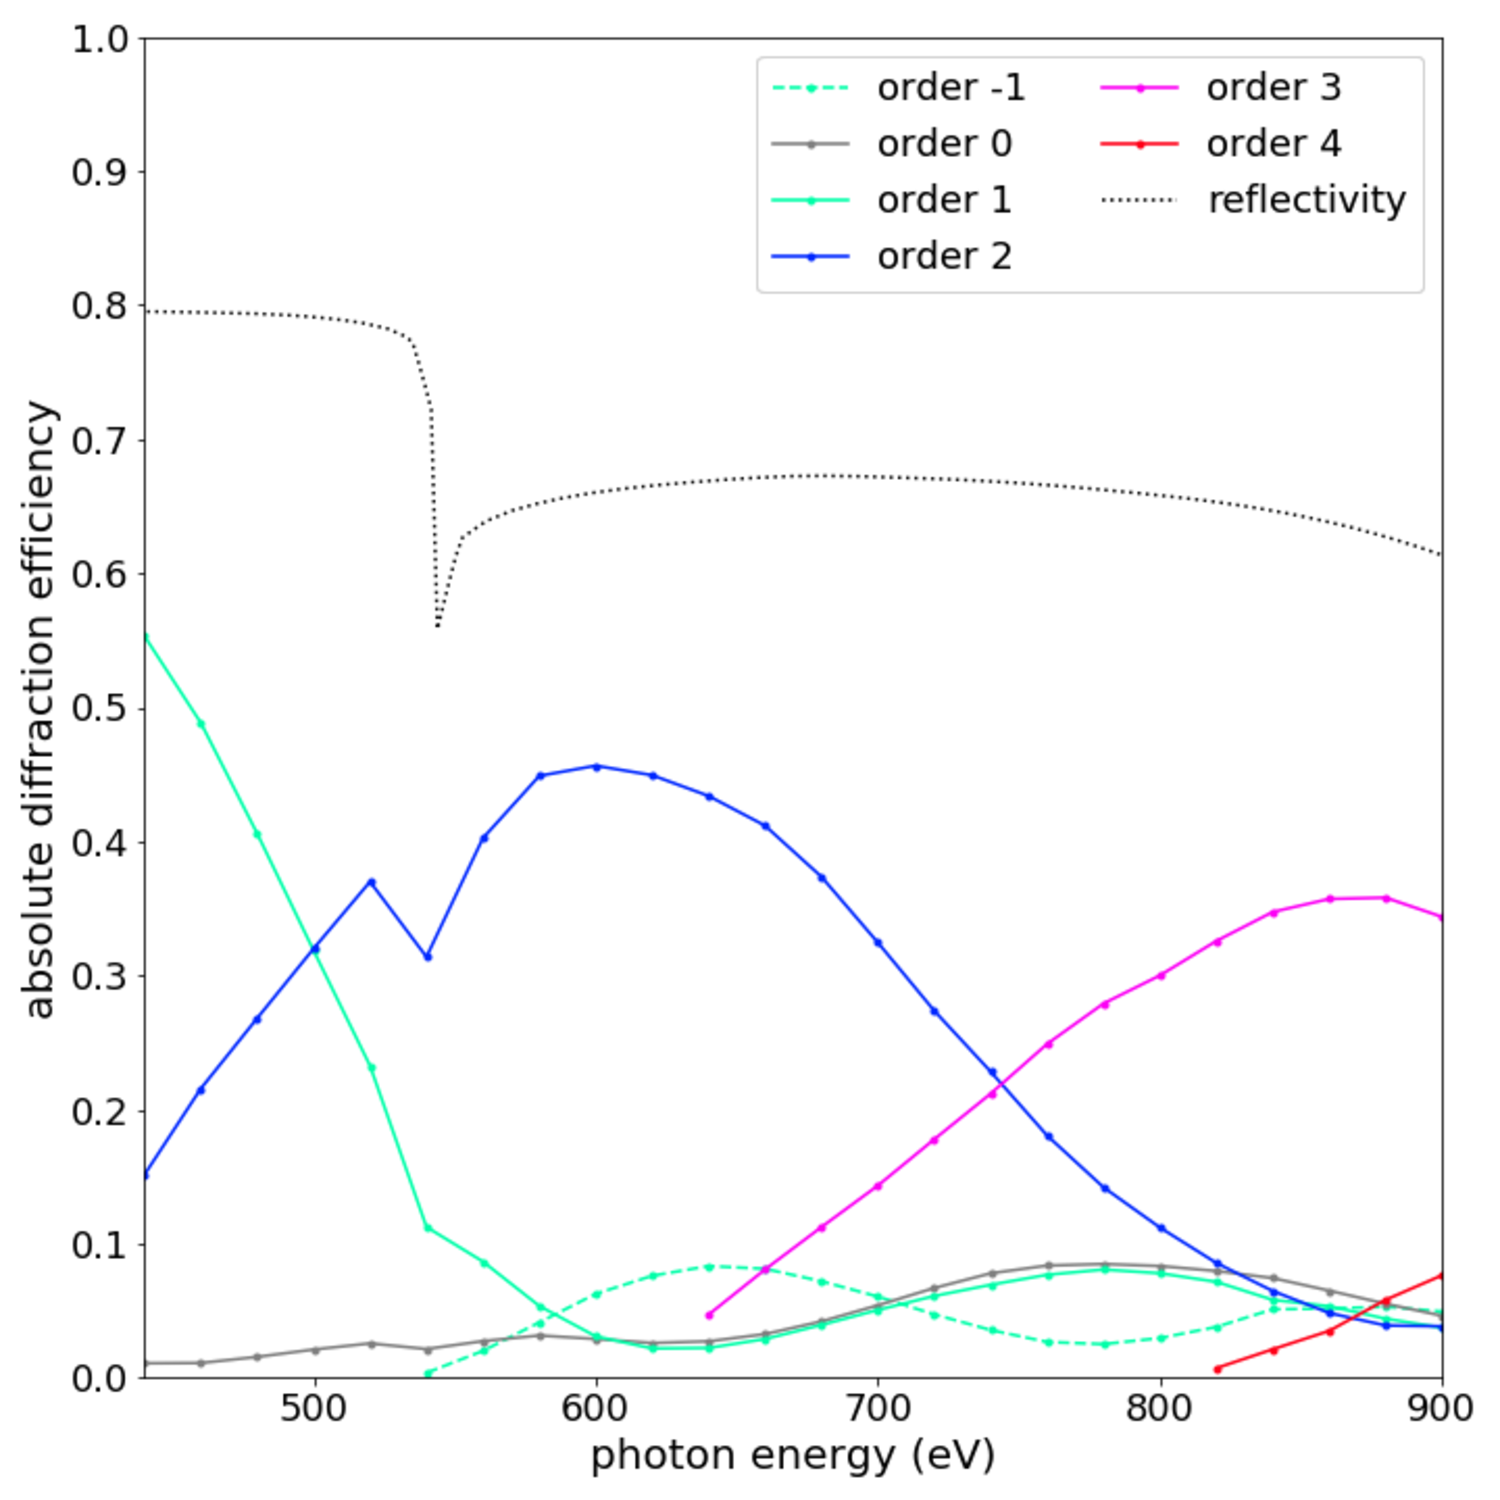
\includegraphics[scale=0.2]{Figures/si_data.pdf}
 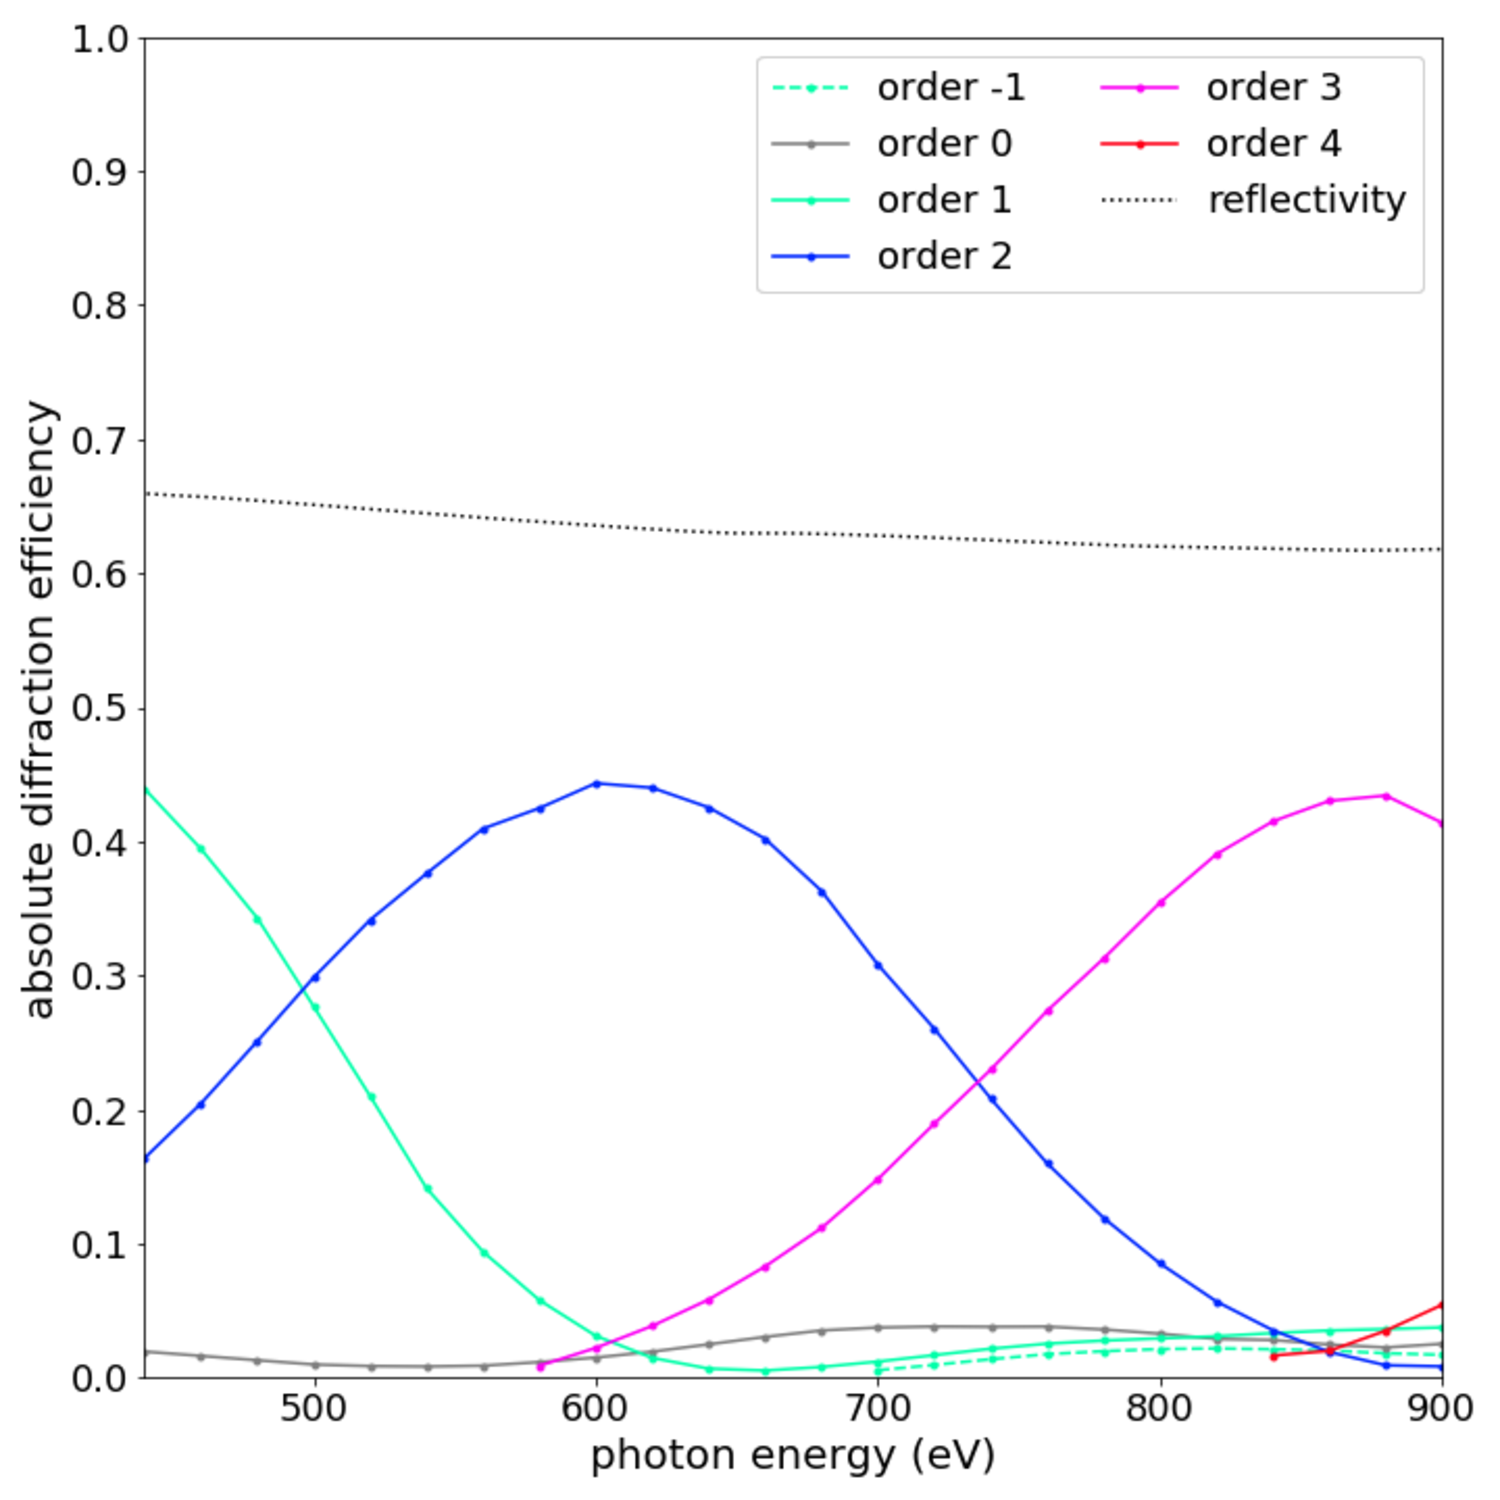
\includegraphics[scale=0.2]{Figures/scil_data.pdf}
 \caption{Measured absolute diffraction efficiency data for silicon master (\emph{left}), coated SCIL replica (\emph{right})}%{Measured absolute diffraction efficiency data for the silicon master (\emph{left}) and the coated SCIL replica (\emph{right}) in geometrical configurations described by the parameters listed in \cref{tab:arc_params} compared to specular reflectivity calculated using the parameters listed in \cref{tab:nom_params}.}\label{fig:abs_eff}
 \end{figure} 
 \vspace{-3mm}
 \centering{$\implies$ Comparable to UV-NIL results (Miles, et al.~2018)}
 \end{minipage}
 \hspace{2mm}
 \begin{minipage}[t]{0.28\linewidth}
  \textbf{Beamline experiments}
  \begin{itemize}
    \item Establish near-Littrow configurations at ALS beamline 6.3.2
    \item Measure $\mathscr{E}_n$ for $n=2,3$ and compare centroids to \textsc{PCGrate-SX} models
    \begin{itemize}
      \item[$\square$] Most sensitive to $\gamma$ and $\delta$ for fixed $d$
    \end{itemize}
  \end{itemize}
  \begin{block}{\footnotesize Blaze wavelength}
    {\quad $\lambda_b \approx \frac{2 d \gamma \sin \left( \delta \right)}{n} \left( 1 - \frac{\left( \delta - \alpha \right)^2}{2} \right)$}
  \end{block}
 \begin{itemize}
  \item Constrain $\delta' / \delta$ to examine impact of resist shrinkage
  \end{itemize}
   %\vspace{-3mm}
 \centering {\footnotesize McCoy, et al.~(2020b)}
 \end{minipage}
\end{frame}

\subsection{Analysis \& Discussion for Resist Shrinkage}


\begin{frame}{Grating Replication by SCIL}
\begin{figure}
 \centering
 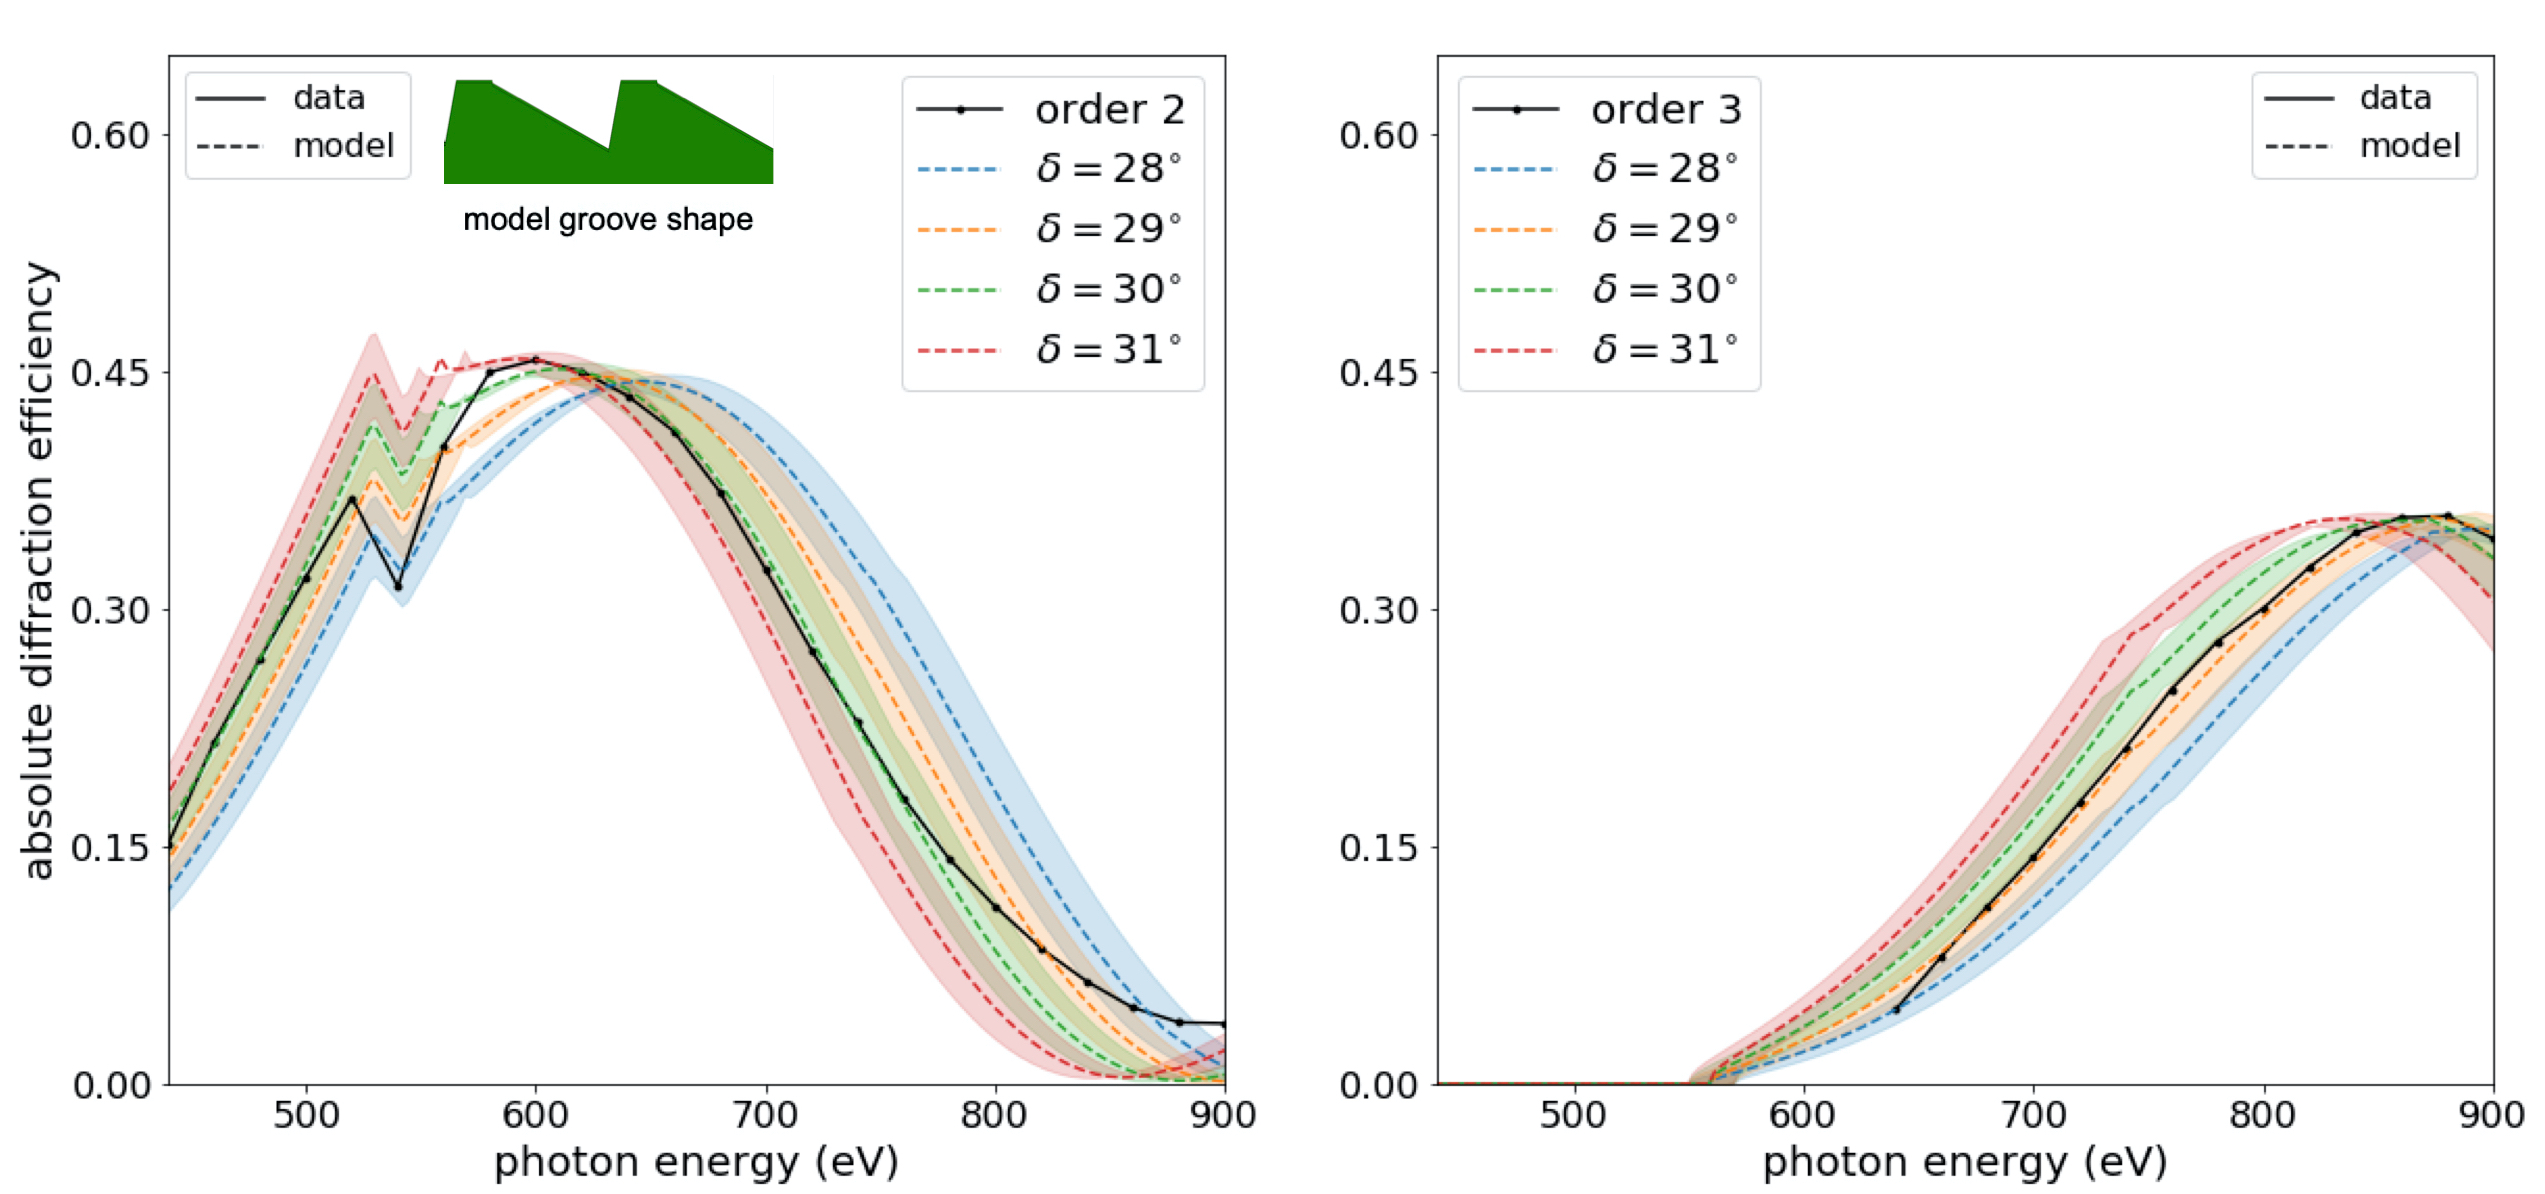
\includegraphics[scale=0.3]{Figures/si_double2.pdf}
 \caption{Measured $\mathscr{E}_n$ in $n=2,3$ for silicon master compared to \textsc{PCGrate-SX} models of varying blaze angle}%{Measured absolute diffraction efficiency data in orders $n=2$ and $n=3$ for the silicon master compared to \textsc{PCGrate-SX} models with $28^{\circ} \leq \delta \leq 31^{\circ}$ that are normalized to match the data in terms of peak efficiency while the shaded swaths represent the $\pm 0.03^{\circ}$ uncertainty in $\gamma$. These results indicate that $\delta$ for the silicon master is close to the value of $\delta = 30^{\circ}$ measured by AFM.}\label{fig:model_si2} 
 \end{figure} 
 \vspace{-5mm}
 \centering{$\implies$ Silicon master close to the nominal value of $\delta = 29.5^{\circ}$}
\end{frame}

\begin{frame}{Grating Replication by SCIL}
\begin{figure}
 \centering
 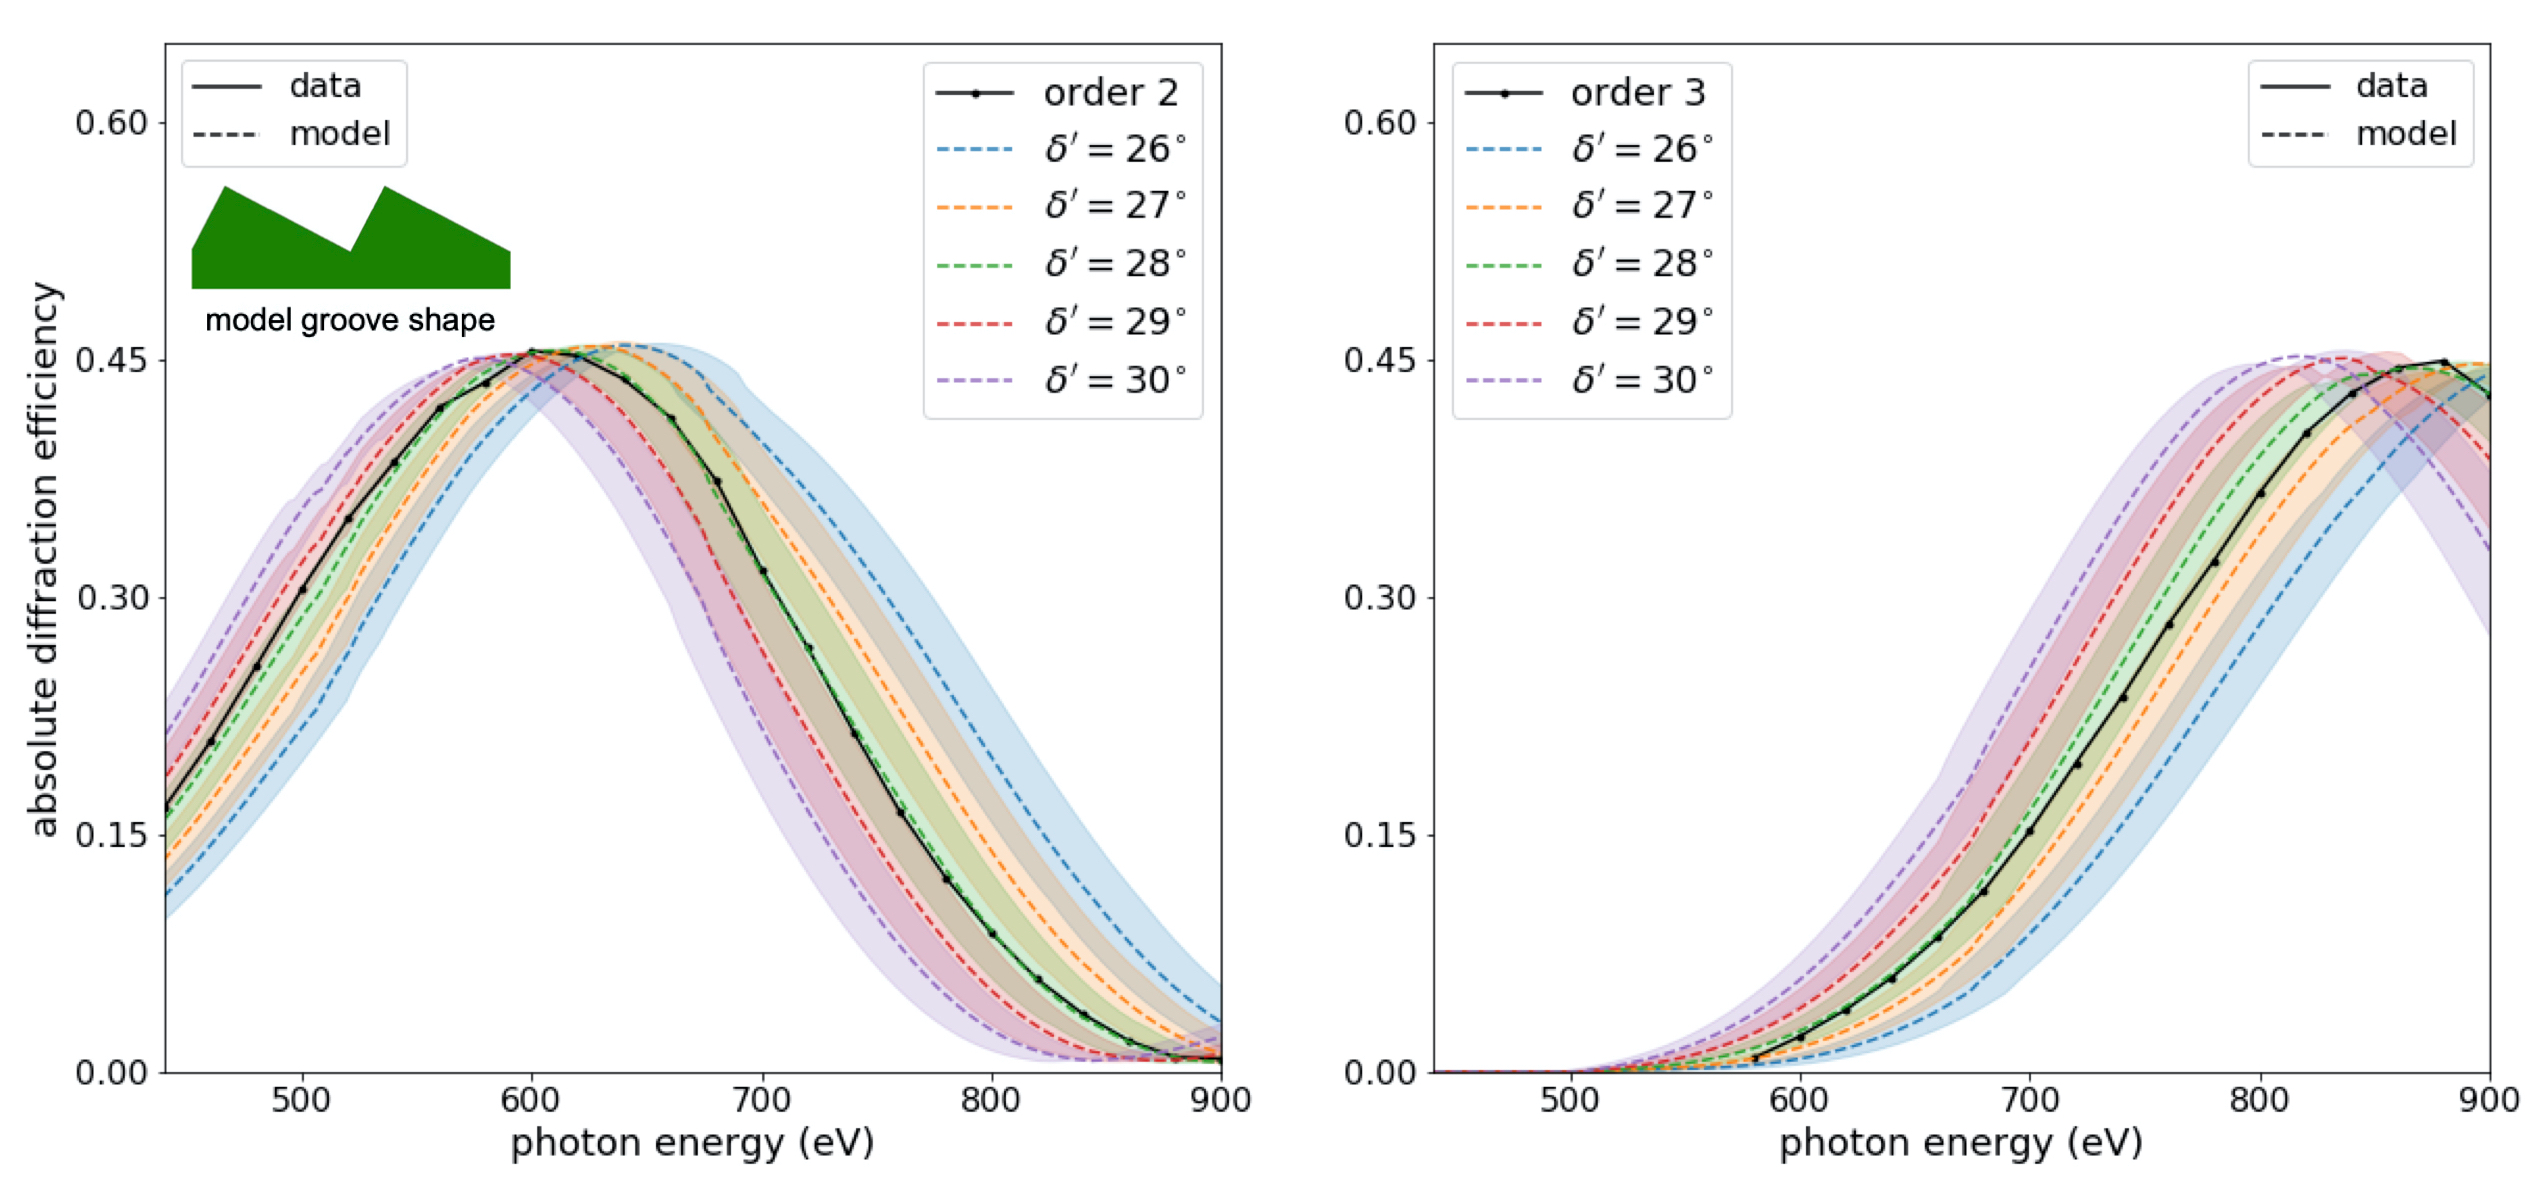
\includegraphics[scale=0.3]{Figures/scil_double2.pdf}
 \caption{Measured $\mathscr{E}_n$ in $n=2,3$ for the silicon master compared to \textsc{PCGrate-SX} models of varying blaze angle}%{Measured absolute diffraction efficiency data in orders $n=2$ and $n=3$ for the silicon master compared to \textsc{PCGrate-SX} models with $28^{\circ} \leq \delta \leq 31^{\circ}$ that are normalized to match the data in terms of peak efficiency while the shaded swaths represent the $\pm 0.03^{\circ}$ uncertainty in $\gamma$. These results indicate that $\delta$ for the silicon master is close to the value of $\delta = 30^{\circ}$ measured by AFM.}\label{fig:model_si2} 
 \end{figure} 
 \vspace{-5mm}
 \centering{$\implies$ Replica closely matches grating with $\delta' = 28^{\circ}$}
\end{frame}

\begin{frame}{Grating Replication by SCIL}
\begin{minipage}[t]{0.47\linewidth}
\vspace{-5mm}
\begin{figure}
 \centering
 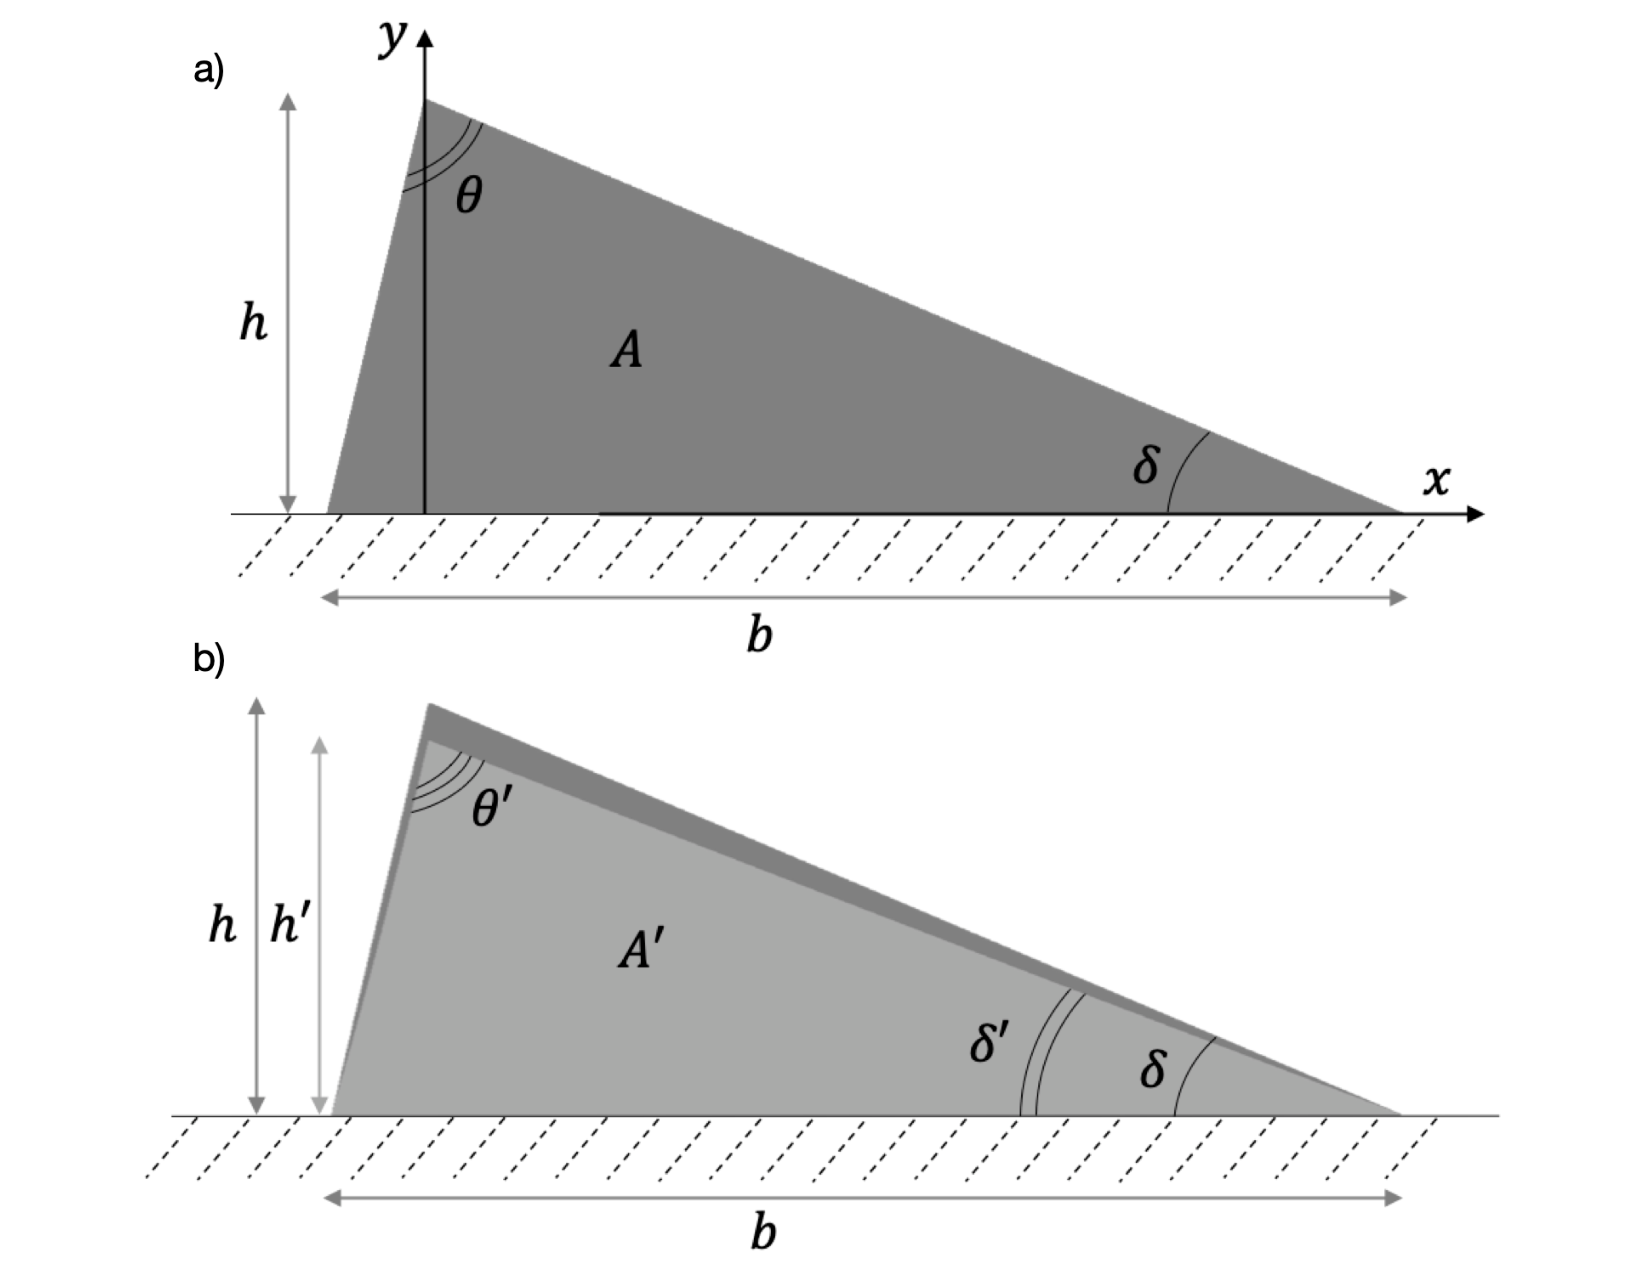
\includegraphics[scale=0.3]{Figures/shrinkage_model_fig.pdf}
 \vspace{-5mm}
 \caption{Approximate model for resist shrinkage with $y = 0$ as fixed boundary defined by residual layer}
 \end{figure}
 \end{minipage}
 \hfill
 \begin{minipage}[t]{0.48\linewidth}
 \textbf{Resist shrinkage}
 \begin{itemize}
  \item Assume inversion of silicon master before shrinkage %Neglect X-PDMS shrinkage in SCIL stamp
    \begin{itemize}
      \item[$\square$] Facet base: $b \approx d - w \lessapprox \SI{130}{\nm}$
      \item[$\square$] Apex angle: $\theta \approx 70.5^{\circ}$ defined by $\{ 111 \}$ planes
      \item[$\square$] Facet angles $\delta$ and $180^{\circ} - \theta - \delta$
    \end{itemize}
  \item Shrinkage w/o boundary: $V' = V (1 - \chi)$
    \begin{itemize}
      \item[$\square$] Residual layer constrained laterally, serves as boundary (Horiba, et al.~2012) %(tens of \si{\nm}) 
      \item[$\square$] {Groove length also constrains shrinkage \newline$\implies$ $A' = A (1 - \chi)$ throughout cross-section}
    \end{itemize}
  \item Shrinkage aspect ratio varies with distance %from boundary
    \begin{itemize}
      %\item[$\square$] Laterally-constrained shrinkage near boundary
      %\item[$\square$] Free shrinkage in $x$, $y$ away from boundary
      \item[$\square$] Assume $S \equiv s_x / s_y = 1 - \mathrm{e}^{-y / \ell_e}$
    \end{itemize}
  \item Divide into 1000 layers, require each to be reduced in area according to
 \end{itemize}
  \centering {$\left( 1 - s_x \right) \left( 1 - s_y \right) = \frac{A'}{A} = \text{const.}$}%{$\frac{A'}{A} = \underbrace{\left( 1 - S f \right)}_{x \text{ shrink}} \underbrace{\left( 1 - f \right)}_{y \text{ shrink}}$}
 \centering {\newline } \vspace{2mm}

 \centering {\footnotesize McCoy, et al.~(2020b)}
  \end{minipage}
\end{frame}

\begin{frame}{Grating Replication by SCIL}
\begin{minipage}[t]{0.50\linewidth}
 \textbf{Resist shrinkage}
  \begin{itemize}
  \item General result
    \begin{itemize}
      \item[$\square$] Decrease in groove depth: $h' < h$
      \item[$\square$] Increase in apex angle: $\theta' > \theta$
      \item[$\square$] Small level of curvature for $y \lessapprox \ell_e$
      \item[$\square$] \textbf{Decrease in blaze angle:} $\delta' < \delta$
    \end{itemize}
  \item $\delta' / \delta$ depends on $\chi$ and $\ell_e$
    \begin{itemize}
      \item[$\square$] $\delta' / \delta \approx 0.93$ consistent with $\chi \approx 0.1$ \& $\ell_e \approx 0.05 h$
      \item[$\square$] $\sim \SI{10}{\percent}$ shrinkage in sol-gel network expected %from $T_{\text{cure}} \approx \SI{90}{\celsius}$
    \end{itemize}
  \item Resist shrinkage in SCIL shifts blaze response %of gratings%performance of blazed gratings in terms of ability to maximize diffraction efficiency for a specific angle 
    \begin{itemize}
      \item[$\square$] Comparable result found for UV-NIL replica from Miles et al.~(2018)
    \end{itemize}
    \vspace{2mm}
  \item[$\implies$] Compensate for effect in master grating to ensure that replicas perform as expected
 \end{itemize}
 \vspace{3mm}
 \centering {\footnotesize McCoy, et al.~(2020b)}
 \end{minipage}
 \hfill
 \begin{minipage}[t]{0.48\linewidth}
 \vspace{-3mm}
 \begin{figure}
 \centering
 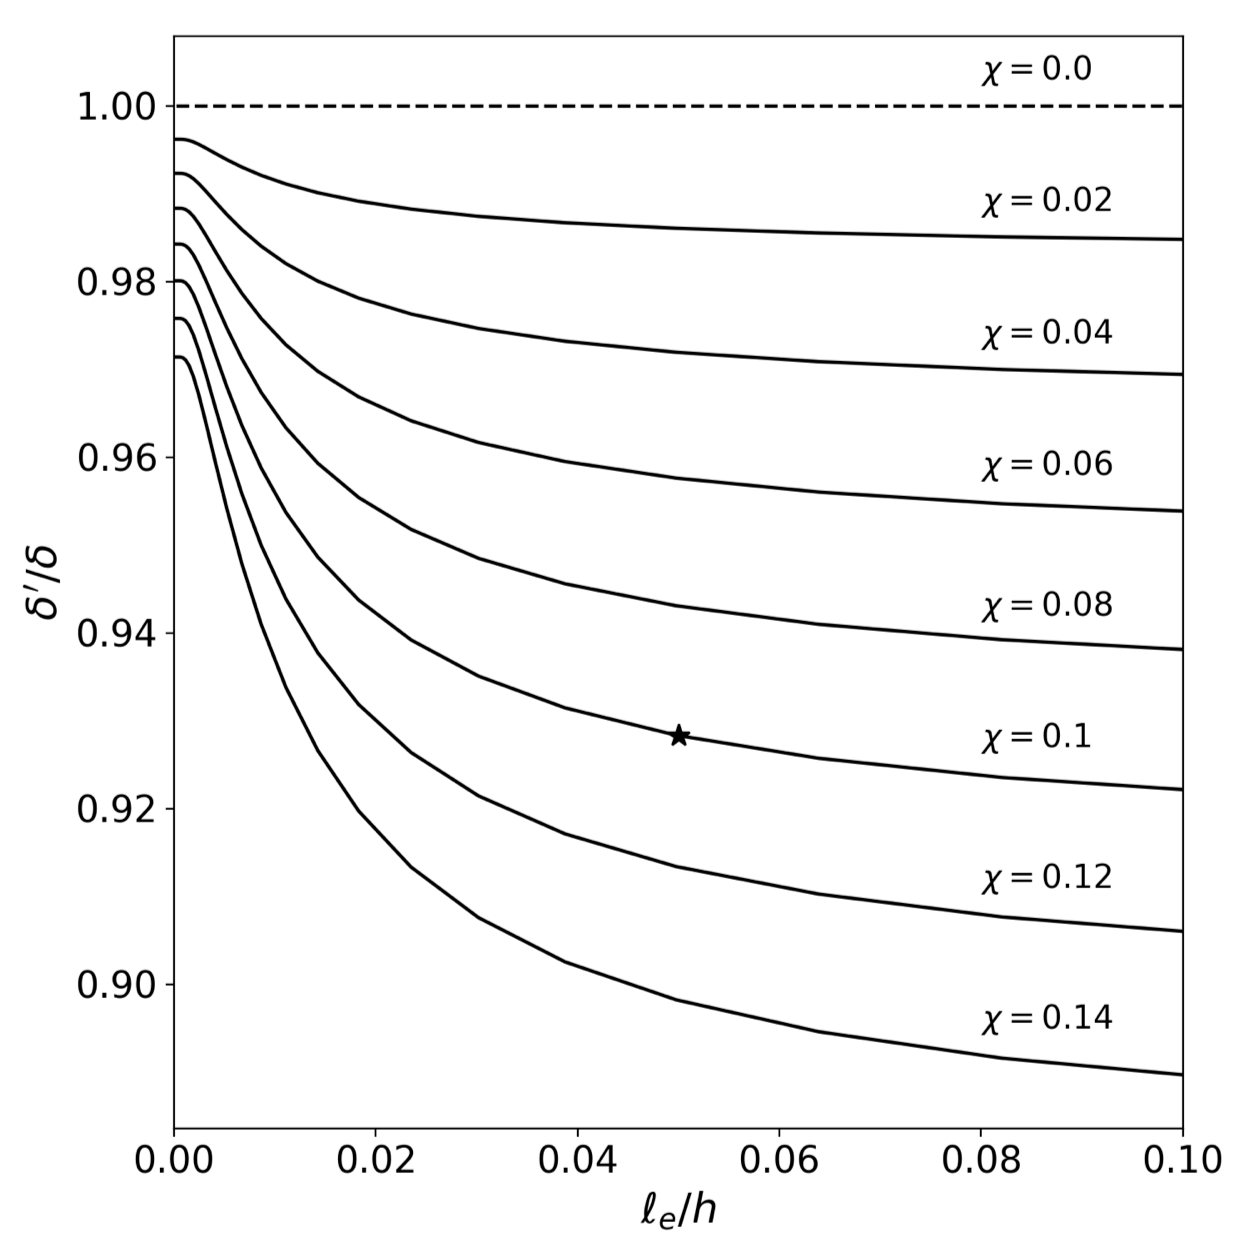
\includegraphics[scale=0.3]{Figures/shrinkage_blaze_plot_edit.pdf} %as a function of various parameters
 \caption{Reduced blaze angle predicted by resist-shrinkage model}%{Reduced blaze angle predicted by the resist-shrinkage model relative to the initial blaze angle, $\delta' / \delta$, as a function of $\ell_e / h$ for various values of $\chi$. With $\chi = 0.1$ and $\ell_e / h = 0.05$ marked by the star, the modeled shrunken facet depicted in \cref{fig:shrinkage} exhibits $\delta' / \delta \approx 0.93$ where $\delta' = 27.4^{\circ}$ and $\delta = 29.5^{\circ}$. }\label{fig:shrinkage_compare} 
 \end{figure}
  \end{minipage}
\end{frame}

\section{Conclusions \& Outlook}

\begin{frame}{Conclusions \& Outlook}
\begin{minipage}[t]{0.48\linewidth}
\vspace{-4mm}
\begin{figure}
\centering
\includegraphics[scale=0.25]{Figures/lynx_art.png}
\end{figure}
\vspace{-2mm}
\begin{exampleblock}{\textbf{X-ray grating fabrication challenges for \emph{Lynx}}}
\begin{enumerate}
  \item Production of a master grating with sawtooth surface-relief profile that enables 
  \begin{itemize}%[label=(\alph*)]
      \item Total absolute diffraction efficiency $> \SI{40}{\percent}$
      \item $\mathscr{R} \gtrapprox 5000$ in a Wolter-I telescope
    \end{itemize}
  %and additionally,  
  \item Mass manufacture of grating replicas to populate modular grating arrays, which involves 
  \begin{itemize}%[label=(\alph*)]
      \item Imprinting grating surface-relief molds 
      \item Coating each replica for soft x-ray reflectivity 
    \end{itemize}
\end{enumerate}
\end{exampleblock}
\end{minipage}
\hfill
\begin{minipage}[t]{0.48\linewidth}
\textbf{Thermally-activated selective topography \newline equilibration (TASTE)}
\begin{itemize}
  \item Couples GEBL with thermal reflow
  \begin{itemize}
    \item[$\square$] Process development at Penn State Nanofab
  \end{itemize}
  \item Eliminates dependence on crystal structure
  \begin{itemize}
    \item[$\square$] Provides way for radially-ruled, blazed grating layout to be generated with EBL precision 
    \item[$\implies$] Enables high $\mathscr{R}$ %by reducing spectral aberrations %from an imperfect radial profile
  \end{itemize}
  \item Meets efficiency requirement
  \end{itemize}
\textbf{Substrate-conformal imprint lithography (SCIL)}
\begin{itemize}
  \item Variant of NIL designed for high-throughput patterning over large areas 
  \begin{itemize}
    \item[$\square$] Equipment for low-volume SCIL recently installed at Penn State Nanofab
  \end{itemize}
  \item Practical for \emph{XGS} reflection grating production
  \begin{itemize}
    \item[$\square$] Compensate blaze angle for resist shrinkage%Resist shrinkage impacts blaze angle
  \end{itemize}
  \item Comparable efficiency to UV-NIL replica
  \end{itemize}
\end{minipage}
\end{frame}

\begin{frame}{Acknowledgments}
This research was supported by the NASA Space Technology Research Fellowship (NSTRF) under grant No.\ NNX16AP92H and used resources of 
\begin{itemize}
  \item The Advanced Light Source (ALS), which is a DOE Office of Science User Facility under contract No.\ DE-AC02-05CH11231
  \item The Nanofabrication Laboratory and the Materials Characterization Laboratory at the Penn State Materials Research Institute
  \item The Quattrone Nanofabrication Facility at the Singh Center for Nanotechnology, University of Pennsylvania
  \item Philips SCIL Nanoimprint Solutions in Eindhoven, Netherlands
  \end{itemize}
%the Advanced Light Source (ALS), which is a DOE Office of Science User Facility under contract No.\ DE-AC02-05CH11231, the Nanofabrication Laboratory and the Materials Characterization Laboratory at the Penn State Materials Research Institute, the Quattrone Nanofabrication Facility at the Singh Center for Nanotechnology, University of Pennsylvania, and Philips SCIL Nanoimprint Solutions in Eindhoven, Netherlands. 
\end{frame}

\begin{frame}[allowframebreaks]{References}

  \nocite{*}
  \bibliography{McCoy-Presentation}
  %\bibliographystyle{plain}
  \bibliographystyle{abbrv}

\end{frame}

\begin{frame}
 \centering
 \frametitle{Flux}
 \framesubtitle{license}
 Flux is licensed under GNU General Public License v3.\\[0.3cm]
  \centering\textbf{http://www.gnu.org/licenses}\\[0.3cm]
Inspired by \textbf{Metropolis} theme from Matthias Vogelgesang.\\
https://github.com/matze/mtheme 
 
\end{frame}




%\begin{frame}{Astrophysical Motivation for Custom Blazed Gratings}
%\begin{minipage}[t]{0.44\linewidth}
%\vspace{-4mm}
%\begin{figure}
% \centering
% 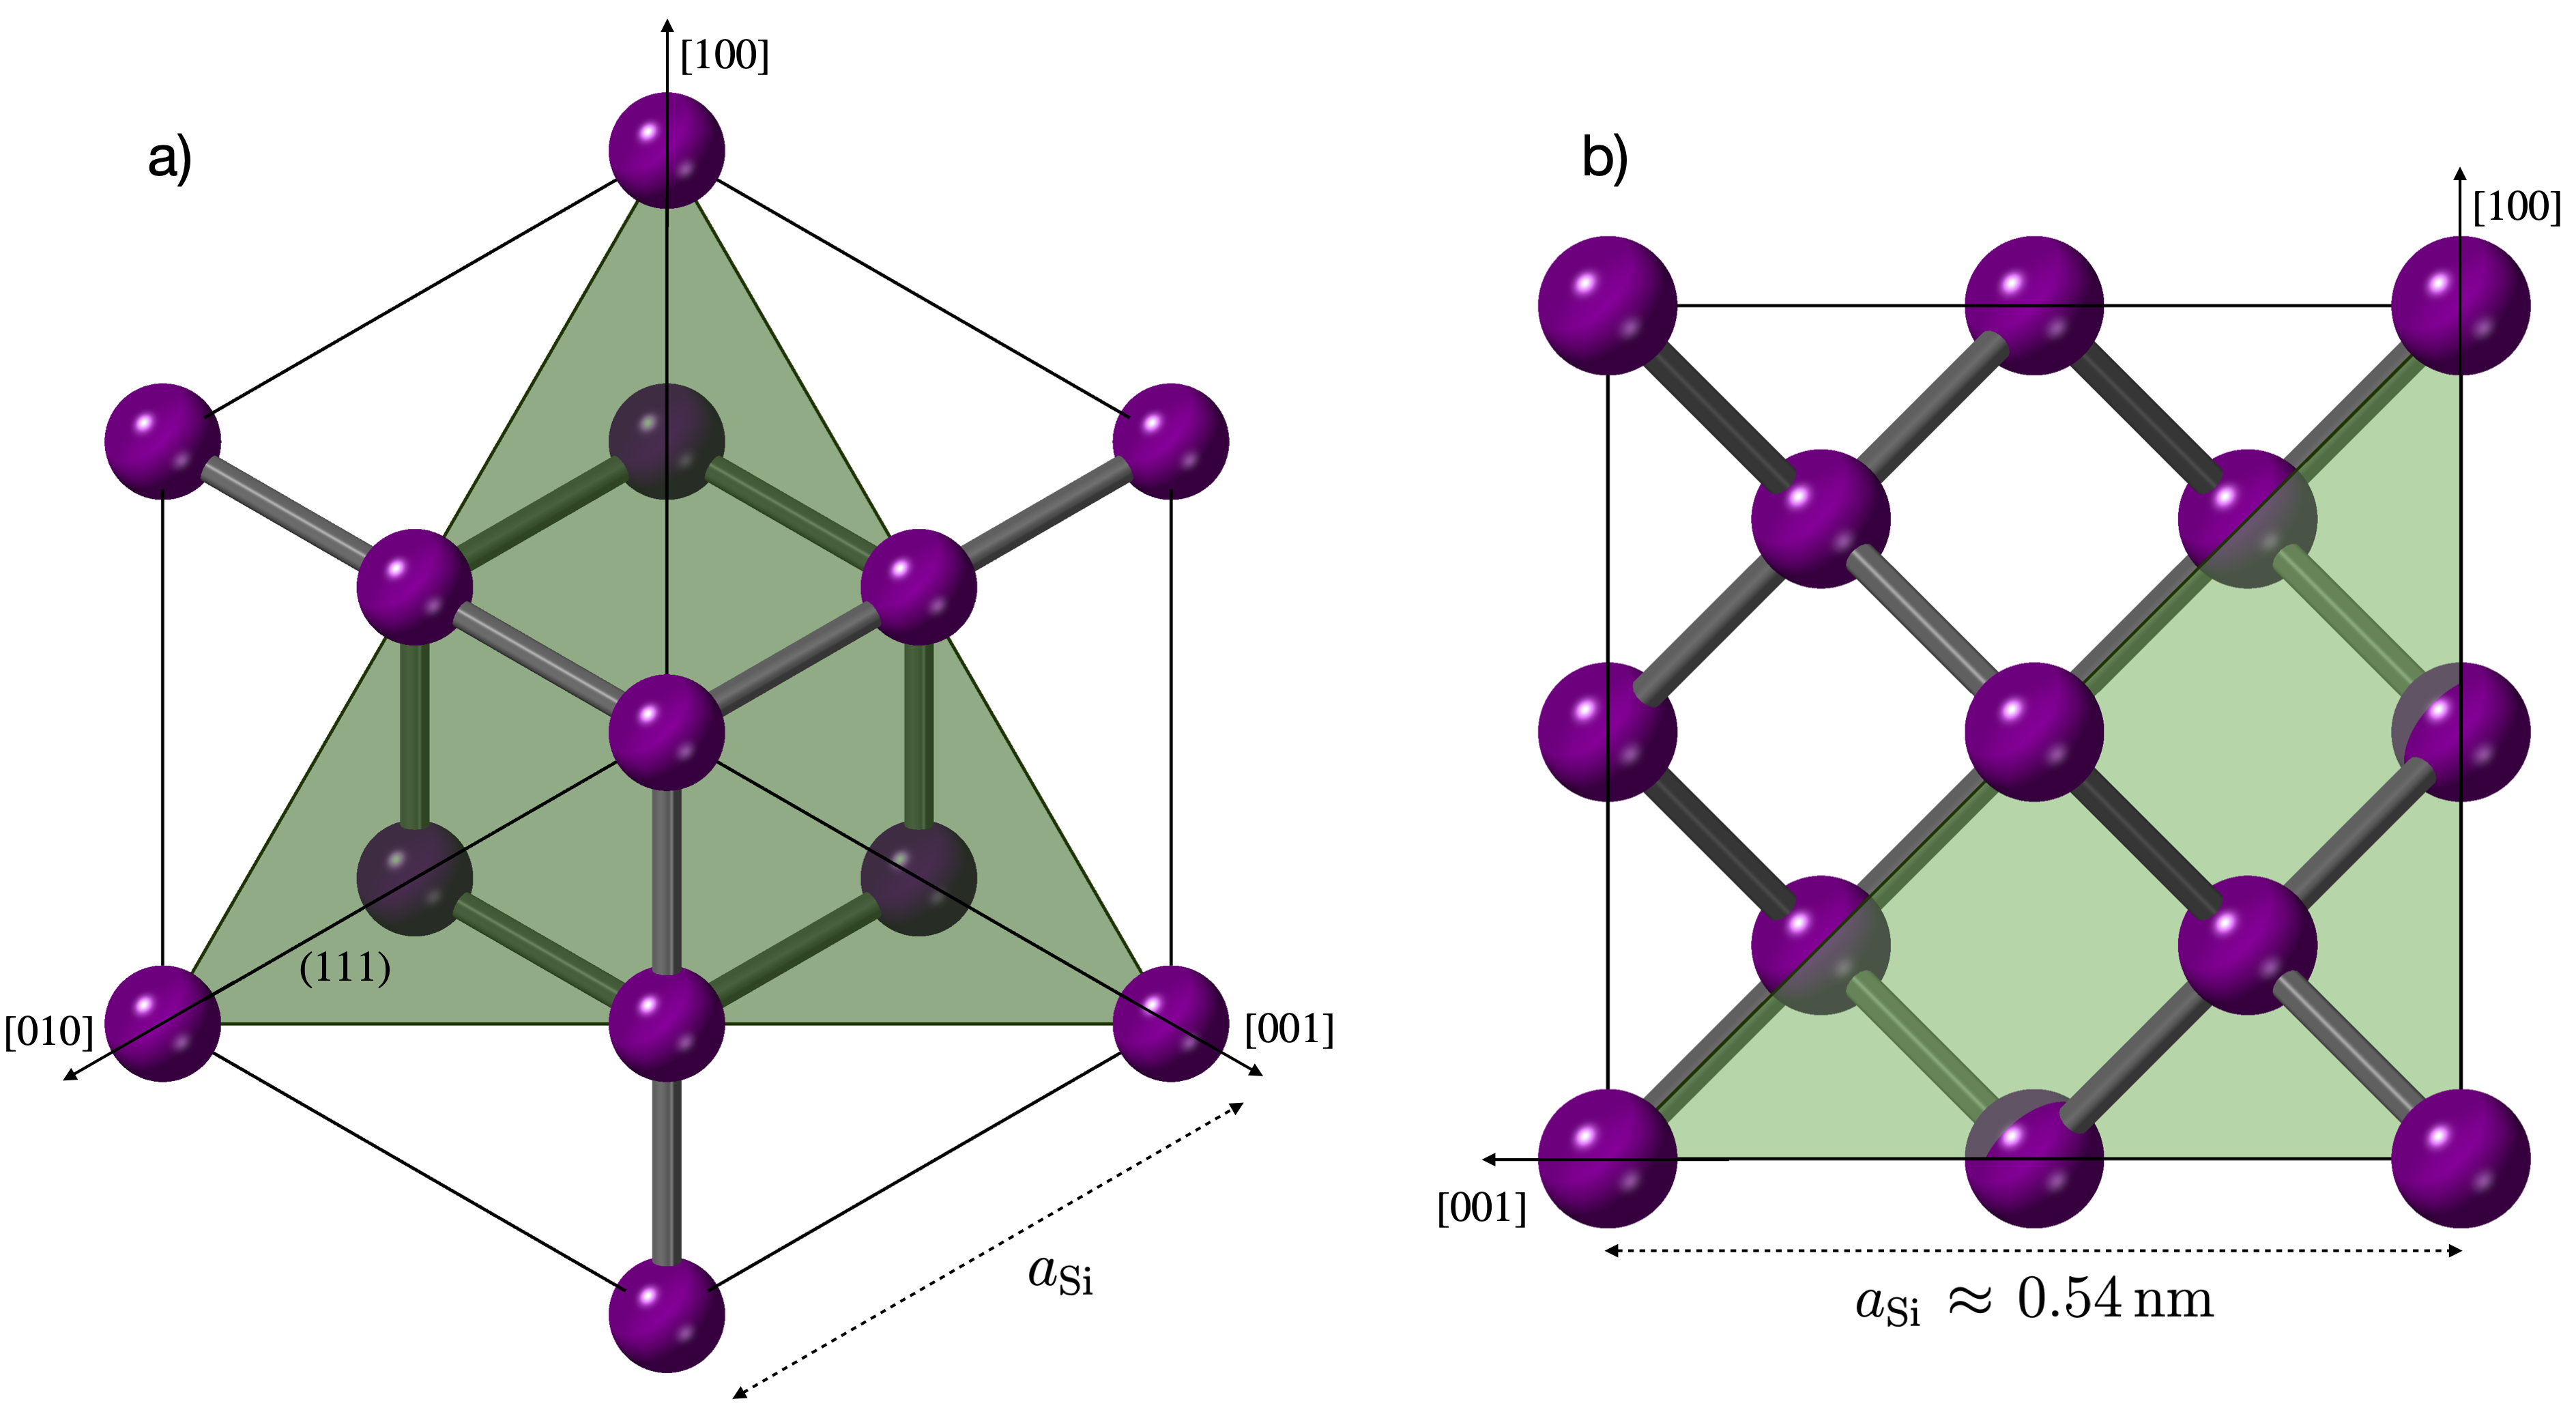
\includegraphics[scale=0.1]{Figures/crystal_fig1.png}
% 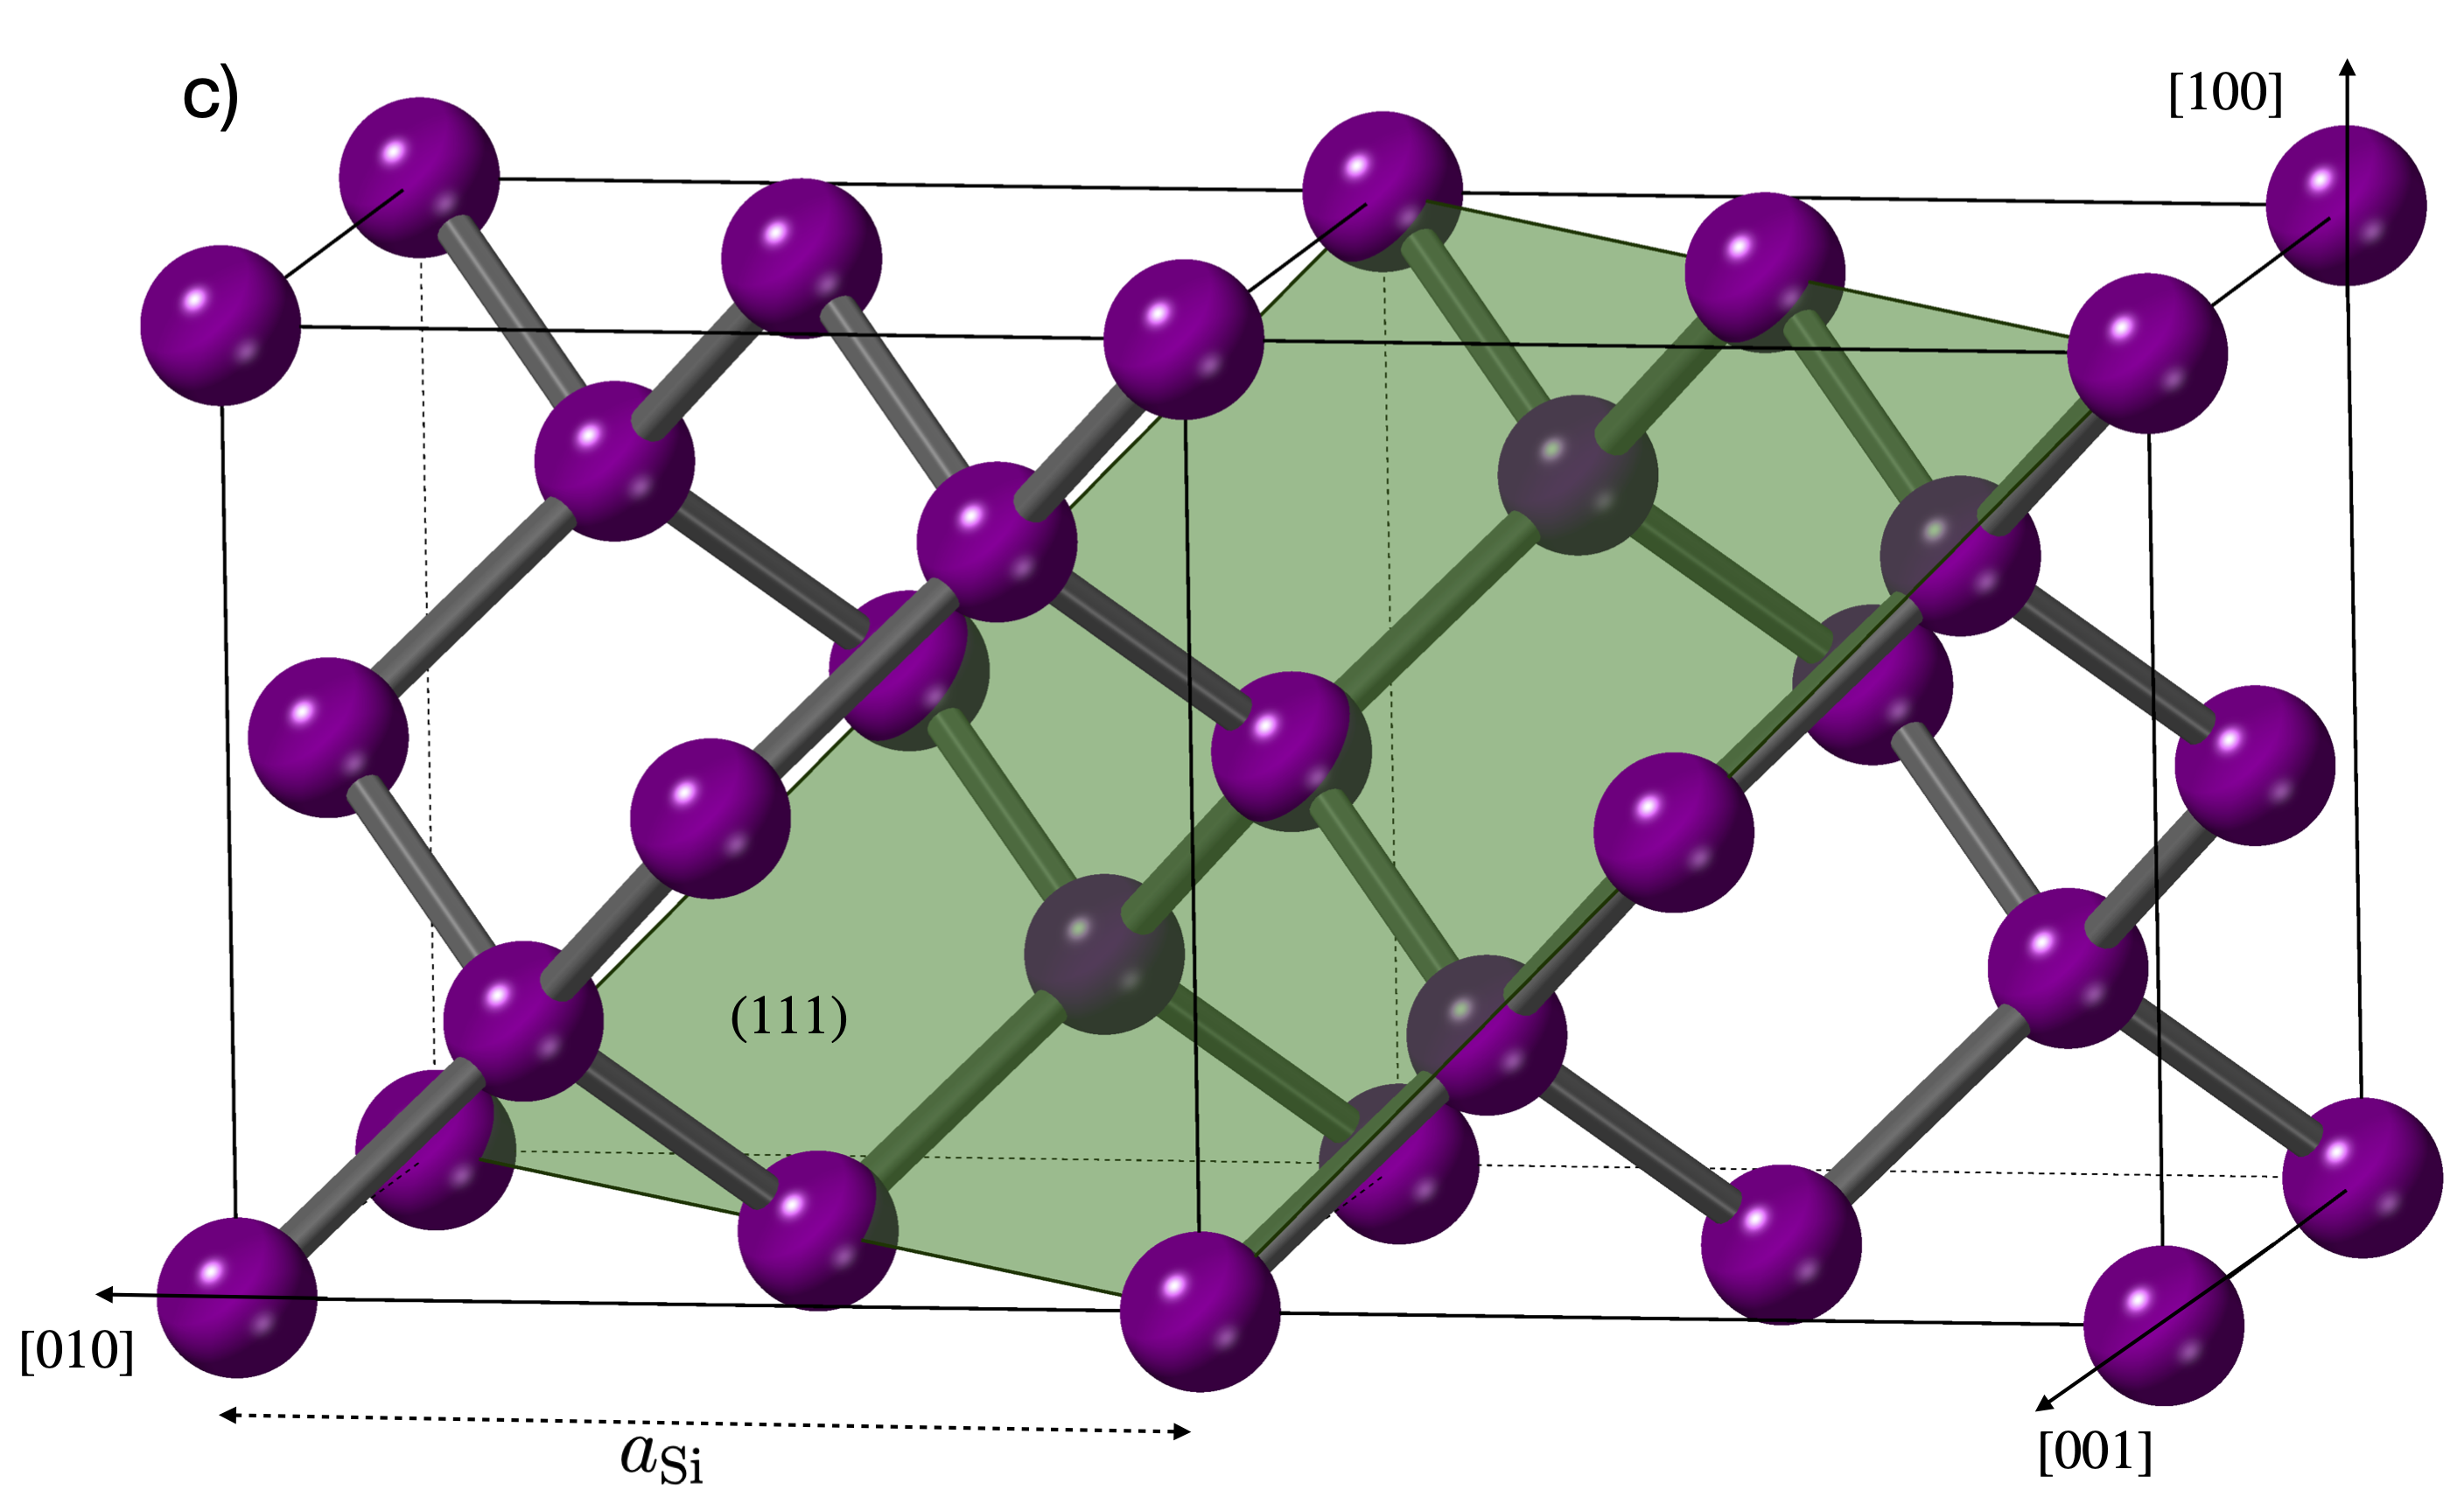
\includegraphics[scale=0.1]{Figures/crystal_fig2.png}
% \caption{Face-centered cubic structure of silicon \newline (T.\ Wood using \textsc{CrystalMaker})}%{Three views of the face-centered cubic structure of silicon where $a_{\text{Si}} \approx \SI{0.54}{\nm}$ is the lattice constant, cube faces are $\{ 100 \}$ planes, purple spheres represent silicon atoms and gray bars indicate covalent bonds while the $(111)$ plane is shown in shaded green: a) down the $[ 111 ]$ axis of a single unit cell, b) down the $[ 010 ]$ axis of a single unit cell and c) two adjacent cells. Image credit: T.\ Wood using \textsc{CrystalMaker X}.}\label{fig:crystal_structure} 
% \end{figure}
% \end{minipage}
%\hfill
%\begin{minipage}[t]{0.54\linewidth}
%\vspace{-5mm}
%\begin{figure}
% \centering
% \includegraphics[scale=0.48]{Figures/UV1.mps}
%  \includegraphics[scale=0.48]{Figures/UV_rev1.mps}
%  \vspace{-3mm}
% \caption{Geometry for \ce{KOH} etching in $\langle 100 \rangle$-oriented silicon (\emph{top}), $\langle 311 \rangle$-oriented silicon (\emph{bottom}) with $[01\overline{1}]$ pointing out of page}%{Geometry for \ce{KOH} etching in a $\langle 100 \rangle$-oriented silicon wafer. The surface of the wafer is a $\{ 100 \}$ equivalent plane with a normal direction taken to be $[100]$. In this projection, the $[01\overline{1}]$ direction points out of the page while $(111)$ and $(1\overline{1} \overline{1})$ are the exposed $\{ 111 \}$ planes, defining an angle $\theta = 70.53^{\circ}$. The result is a symmetric sawtooth with a nominal blaze angle $\delta = 54.74^{\circ}$.}\label{fig:KOH_geo}
% \end{figure}
% \vspace{-5mm}
% \begin{block}{\footnotesize \emph{Crystallographic etching}}
% \centering
% {Choice of wafer orientation determines facet angles $\delta$ and $\bar{\delta} = 180^{\circ} - \theta - \delta$ with $\theta \approx 70.5^{\circ}$}
% \end{block}
% \end{minipage}
%\end{frame}

%\begin{frame}{Beamline Characterization of Diffraction Efficiency}
%\begin{minipage}[t]{0.48\linewidth}
%\vspace{-4mm}
%\begin{figure}
% \centering
% 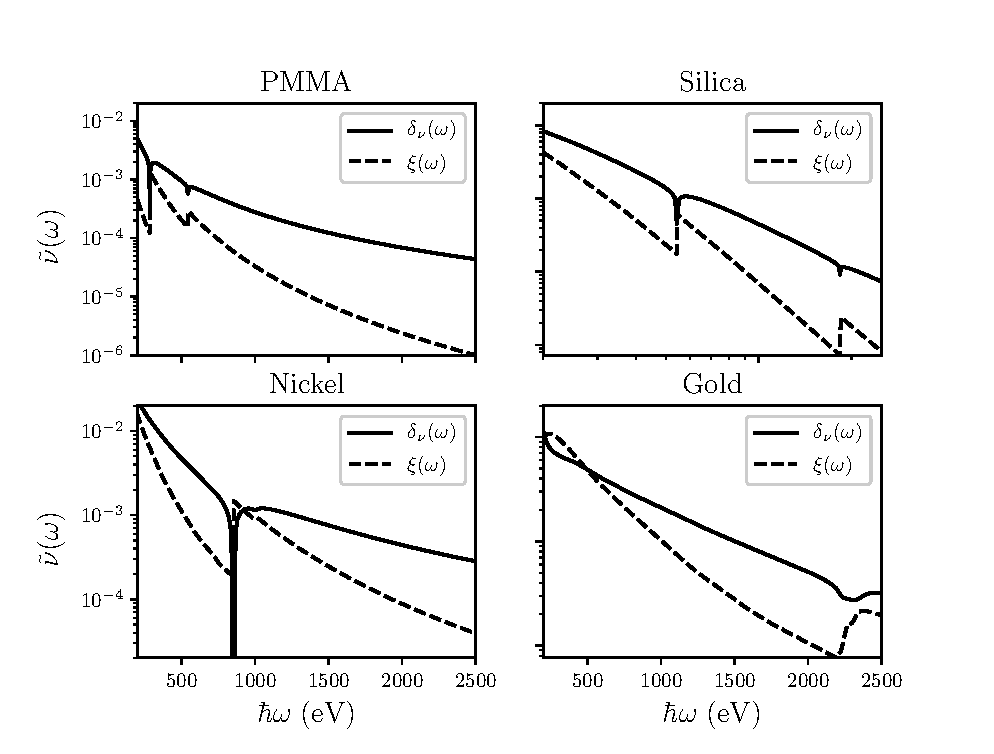
\includegraphics[scale=0.48]{Figures/X-ray_index.eps}
% \caption{Soft x-ray index of refraction (from CXRO)}\label{fig:X-ray_index} 
% \end{figure}
% \vspace{-4mm}
% \centering {$\tilde{\nu}(\omega) \equiv 1 - \delta_{\nu} (\omega) + i \xi(\omega)$}
 %{\quad \quad \quad \quad \quad $\tilde{\nu}(\omega) \equiv 1 - \delta_{\nu} (\omega) + i \xi(\omega)$}
% \end{minipage}
%\hfill
%\begin{minipage}[t]{0.48\linewidth}
%\vspace{-4mm}
%\begin{figure}
% \centering
% 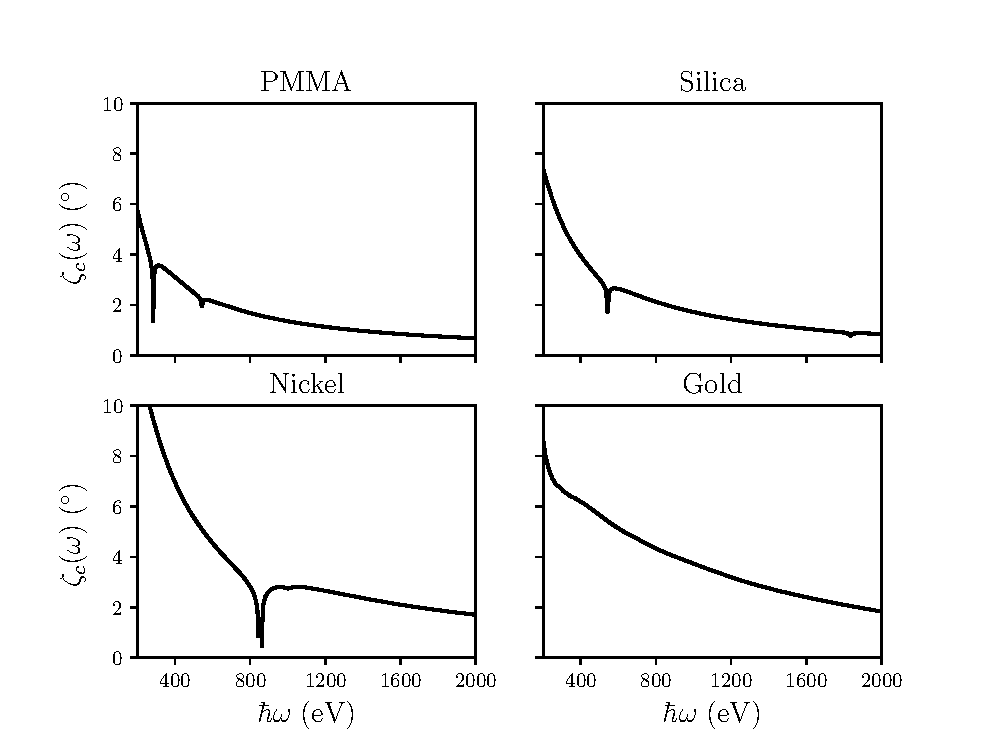
\includegraphics[scale=0.48]{Figures/critical_angle.eps}
% \caption{Critical angle for total external reflection}\label{fig:critical_angle}
% \end{figure}
% \vspace{-4mm} 
% \centering {$1 - \delta_{\nu} (\omega) \lessapprox 1 \implies \zeta_c (\omega) \approx \sqrt{2 \delta_{\nu} (\omega)}$}
 %{\quad \quad \quad $1 - \delta_{\nu} (\omega) \lessapprox 1 \implies \zeta_c (\omega) \approx \sqrt{2 \delta_{\nu} (\omega)}$}
% \end{minipage}
%\end{frame}

%\begin{frame}{Beamline Characterization of Diffraction Efficiency}
%\begin{minipage}[t]{0.48\linewidth}
%\begin{figure}
% \centering
% 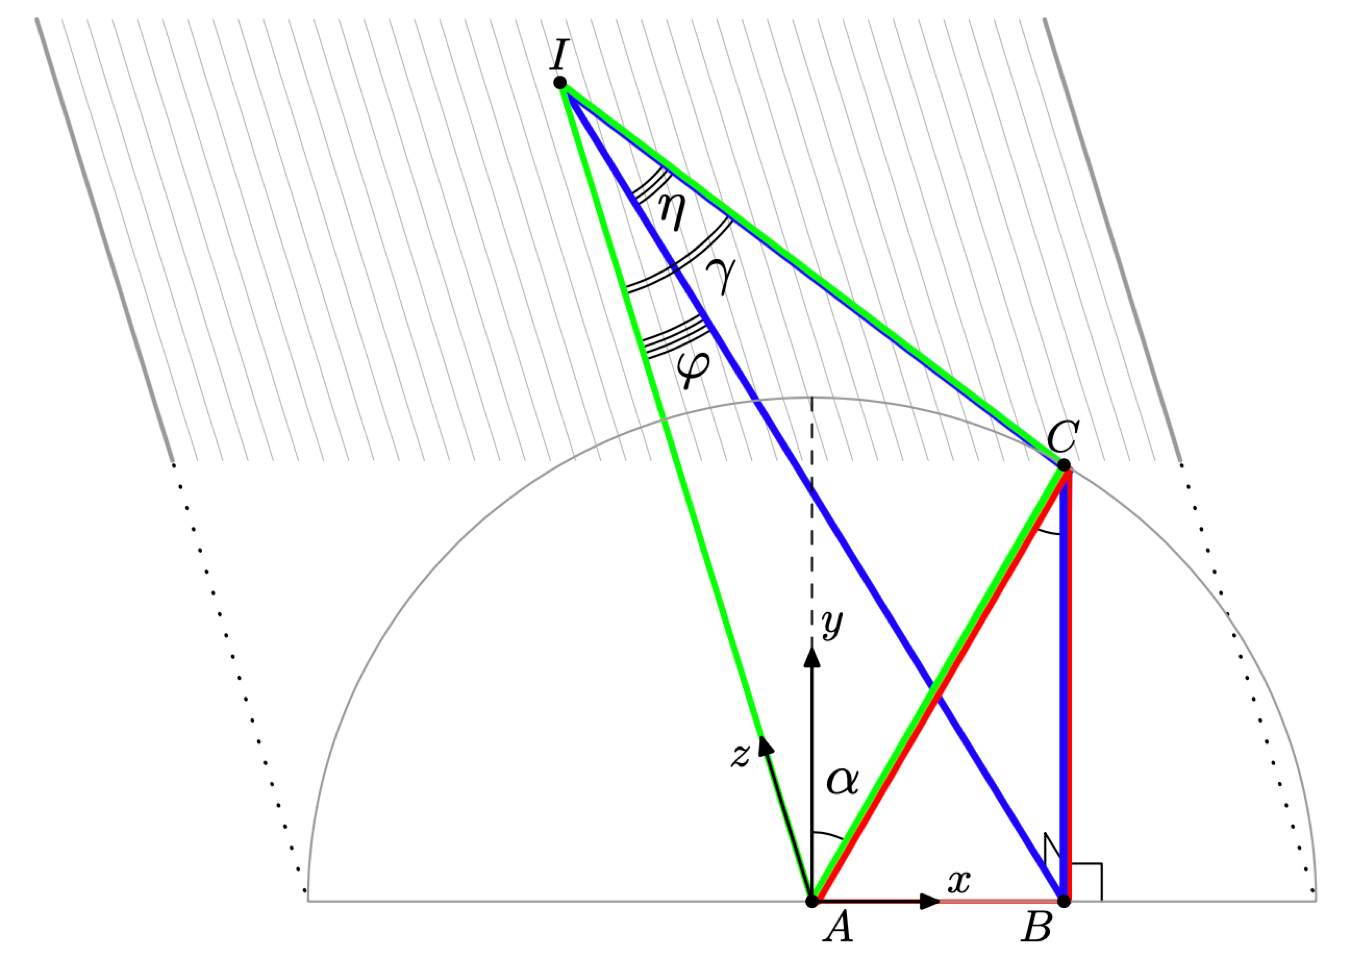
\includegraphics[scale=0.25]{Figures/grating_angles.pdf}
% \caption{Angles relevant for beamline diffraction-efficiency testing: $\alpha \equiv \angle ACB$, $\gamma \equiv \angle AIC$, $\eta \equiv \angle CIB$ and $\varphi \equiv \angle AIB$}%{Angles relevant for beamline diffraction-efficiency testing. The grating incidence angles $\alpha \equiv \angle ACB$ and $\gamma \equiv \angle AIC$ introduced in \cref{fig:conical_reflection_edit} are controlled through rotations about principal axes, which are parametrized by the angles $\eta \equiv \angle CIB$ and $\varphi \equiv \angle AIB$ given by \cref{eq:graze_angle,eq:yaw_angle}.}\label{fig:grating_angles} 
% \end{figure} 
% \end{minipage}
% \hfill
%\begin{minipage}[t]{0.48\linewidth}
%\begin{equation}\label{eq:graze_angle}
% \sin \left( \eta \right) = \sin \left( \gamma \right) \cos \left( \alpha \right)
 %\end{equation}
 %\begin{equation}\label{eq:yaw_angle}
 %\sin \left( \varphi \right) = \tan \left( \alpha \right) \tan \left( \eta \right) 
 %\end{equation}
 %\end{minipage}
%\end{frame}

%\begin{frame}{Beamline Characterization of Diffraction Efficiency}
%\begin{minipage}[t]{0.48\linewidth}
%\begin{equation}\label{eq:arc_circle} 
% \left( x - x_{\text{cen}} \right)^2 + \left( y - y_{\text{cen}} \right)^2 = r^2 %\ \ \text{with} \\ r = L \sin (\gamma),
% \end{equation}
% \begin{equation}\label{eq:measure_gamma}
% \gamma = \arcsin \left( \frac{r}{L} \right) \approx \frac{r}{L} , % + \frac{1}{6} \left( \frac{r}{L} \right)^3 ,
% \end{equation}
% \begin{equation}\label{eq:measure_alpha}
% \alpha = \arcsin \left( \frac{\Delta x_{\text{dir}}}{r} \right) ,
% \end{equation}
% \begin{equation}\label{eq:measure_roll}
% \phi = \arcsin \left( \frac{\Delta x_0}{r} \right) - \alpha \approx \frac{\Delta x_0}{r} - \sin \left( \alpha \right) ,
% \end{equation}
% \end{minipage}
% \hfill
%\begin{minipage}[t]{0.48\linewidth}
%\begin{figure}
% \centering
% 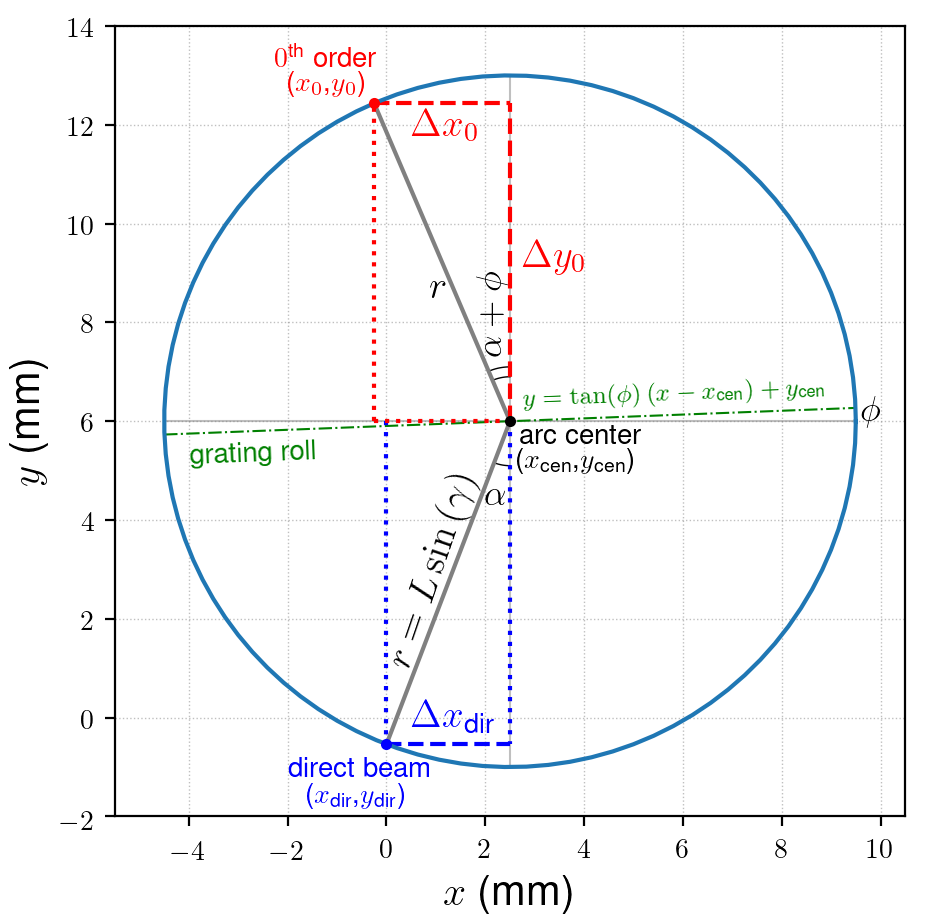
\includegraphics[scale=0.5]{Figures/arc_example.png}
% \caption{Example of diffracted arc fit to circle with radius $r$ and arc center $(x_{\text{cen}},y_{\text{cen}})$ from gathered $(x_n,y_n)$ data.}%{Example of a diffracted arc fit to a circle by \cref{eq:arc_circle} with radius $r$ and arc center $(x_{\text{cen}},y_{\text{cen}})$ from gathered $(x_n,y_n)$ data. The cone opening half-angle, $\gamma$, is related to the system throw, $L$, through $r = L \sin \left( \gamma \right)$ while the azimuthal incidence angle, $\alpha$, follows from $\sin \left( \alpha \right) = \Delta x_{\text{dir}}/r$, where $\Delta x_{\text{dir}}$ is the $x$-distance between $x_{\text{cen}}$ and the direct beam. Grating roll, $\phi$, can be constrained using $\sin \left( \alpha + \phi \right) = \Delta x_0/r$, where $\Delta x_0$ is the $x$-distance between $x_{\text{cen}}$ and $0^{\text{th}}$ order. By \cref{eq:measure_graze}, the substrate graze angle, $\eta$, can be determined using the $y$-distance between $y_{\text{cen}}$ and $0^{\text{th}}$ order, $\Delta y_0$, while the angle for grating yaw, $\varphi$, follows from \cref{eq:measure_yaw}.}\label{fig:ALS_arc}
% \end{figure}
% \end{minipage}
%\end{frame}

%\begin{frame}{Beamline Characterization of Diffraction Efficiency}
%Calculating theoretical diffraction efficiency by the integral method involves the following mathematical steps:
%\begin{enumerate}
% \item The inhomogeneous Helmholtz equation, $\left( \nabla_{xy}^2 + k_{xy}^2 \right) E_z'' (x,y) = - i \mu_0 \omega \mathcal{J}_z (x,y)$, is solved for the case of a point-source grating using \emph{Green's functions}.
% \item An expression for $E_z'' (x,y)$ is formulated as the convolution of the appropriate Green's function and $\mathscr{J}_z (x)$, where $\mathscr{J}_z (x) \mathrm{e}^{-i k_x x} = \sum_{n=-\infty}^{\infty} \mathscr{J}_{z,n} \mathrm{e}^{i n K x}$%defined by \cref{eq:surf_curr_expan}.
% \item A \emph{Dirichlet boundary condition} for TE polarization is enforced on $\mathcal{P}$ to yield a system of coupled integrals that can be solved numerically to determine $\mathscr{J}_{z,n}$ for a truncated range of $n$.
% \item The expression for $E_z'' (x,y)$ is truncated accordingly and the amplitude of each propagating order is found using calculated values for $\mathscr{J}_{z,n}$. 
% \item The amplitudes for each propagating order are used to calculate diffraction efficiency, $\mathscr{E}_n$, in TE polarization. Due to the assumption of perfect conductivity, however, this quantity is equivalent to relative diffraction efficiency with $\sum_n \mathscr{E}_n = 1$ over propagating orders. 
% \item Absolute diffraction efficiency is determined by modulating the results for relative diffraction efficiency by an appropriate expression for soft x-ray reflectivity from a mirror flat %using the framework presented in \cref{sec:planar_interface}. 
% \end{enumerate}
%\end{frame}

%\begin{frame}{Grating Fabrication by TASTE}
%\begin{figure}
% \centering
 %\includegraphics[scale=0.6]{Figures/taste_fab1.mps}
 %\includegraphics[scale=0.6]{Figures/taste_fab2.mps}
 %\includegraphics[scale=0.6]{Figures/taste_fab3.mps}
% \includegraphics[scale=0.6]{Figures/taste_fab4.mps}
% \includegraphics[scale=0.6]{Figures/taste_fab5.mps} %thermally-activated selective topography equilibration (TASTE)
% \caption{\emph{Selective topography equilibration} in TASTE}%{Physical properties of PMMA resist processed by GEBL that enable TASTE. Dose-modulated electron exposure gives rise to a lateral gradient in $M_w$ so that varying resist thicknesses result from $M_w$-dependent etch rates that occur during wet development. The GEBL-fabricated structure also exhibits a lateral gradient in $T_g$, thereby enabling selective thermal reflow at a temperature $T_{g,0} > T > T_{g,1}$ that smooths the exposed staircase steps into a quasi-linear slope. The end result emulates a blazed grating with a groove spacing $d$ and a blaze angle $\delta$.}\label{fig:TASTE_diagram}
% \end{figure}
% \textbf{Selective thermal reflow}
% \begin{itemize}
%  \item Lateral $T_g$ gradient enables selective thermal reflow at $T_{g,0} > T > T_{g,1}$
%  \item Exposed staircase steps become molten while unexposed resists retains glass state
%  \item Time-dependent \emph{visco-elastic creep} process ideally smooths exposed resist into quasi-linear slope 
%  \item End result emulates blazed grating with $d$ and $\delta$ determined from GEBL structure 
% \end{itemize}
%\end{frame}

%\begin{frame}{Grating Fabrication by TASTE}
%\begin{minipage}[t]{0.52\linewidth}
%Change in polarization for a wavelength $\lambda$ can be parameterized through $\Psi$ and $\Delta$ defined by 
%\begin{equation}
% \tan \left( \Psi \right) \mathrm{e}^{i \Delta} = \frac{\tilde{r}_p}{\tilde{r}_s} , 
% \end{equation}
%where $\tilde{r}_s$ and $\tilde{r}_p$ are complex reflection coefficients in s and p polarizations. 
%The reflection coefficient for a thin film of thickness $\tau_2$ on a substrate with an incidence angle $\theta$ is given by \emph{Airy's formula}:
%\begin{equation}\label{eq:refl_coeff_example}
% \tilde{r} = \frac{\tilde{r}_{1,2} + \tilde{r}_{2,3} \mathrm{e}^{-2 i \tilde{k}_{y,2} \tau_2}}{1 + \tilde{r}_{1,2} \tilde{r}_{2,3} \mathrm{e}^{-2 i \tilde{k}_{y,2} \tau_2}} 
% \end{equation} 
%where $\tilde{k}_{y,2}$ is the component of the wave vector perpendicular to surface, in the film while $\tilde{r}_{1,2}$ and $\tilde{r}_{2,3}$ are the reflection coefficients for the two interfaces, in either s or p polarization. % \cite{Tompkins05,Born80,Gibaud2009}. 
%When $\Psi$ and $\Delta$ are measured at $\theta$ near the \emph{Brewster's angle} for the interface between air and the top layer, data are sensitive to $\tau_2$. %, so that with knowledge of the index of refraction for each layer, $\tau_2$ can be determined. 
%\end{minipage}
%\hfill
%\begin{minipage}[t]{0.45\linewidth}
%\begin{figure}
% \centering
% \includegraphics[scale=0.5]{Figures/diffraction_arc27.mps}
% \caption{Geometry for spectroscopic ellipsometry of a film of thickness $\tau_2$ coated on a substrate, in air}%{Geometry for SE of a film of thickness $\tau_2$ coated on a substrate, in air. The index of refraction in air, the film, and the substrate are given by $\nu_1$, $\tilde{\nu}_2$ and $\tilde{\nu}_3$, respectively, so that the corresponding wave vectors in each region are $\mathbold{k}_1$, $\tilde{\mathbold{k}}_2$ and $\tilde{\mathbold{k}}_3$, where $\nu_1$ and $\mathbold{k}_1$ are assumed to be real. The component of $\mathbold{k}_1$ perpendicular to the surface is related to the angle $\theta$: $k_{y,1} = -k_0 \nu_1 \cos \left( \theta \right)$ with $k_0 \equiv 2 \pi / \lambda$ as the wave number in vacuum. By Snell's law, the corresponding components of $\tilde{\mathbold{k}}_2$ and $\tilde{\mathbold{k}}_3$ are given by $\tilde{k}_{y,2} = -k_0 \sqrt{\tilde{\nu}_2^2 - \nu_1^2 \sin^2 \left( \theta \right)}$ and $\tilde{k}_{y,3} = -k_0 \sqrt{\tilde{\nu}_3^2 - \tilde{\nu}_2^2 \sin^2 \left( \theta \right)}$, respectively.}\label{fig:2DSE} 
% \end{figure}
% \end{minipage}
%\end{frame}

%\begin{frame}{Grating Fabrication by TASTE}
%\begin{minipage}[t]{0.46\linewidth}
% \textbf{GEBL process development}
% \begin{itemize}
%  \item \SI{130}{\nm}-thick resist attained by spin-coating PMMA with $M_w = \SI{950}{\kilogram\per\mole}$ (diluted \SI{3}{\percent} in Anisole) onto silicon wafer at 3000 krpm %s \SI{100}{\mm} in diameter %and \SI{0.5}{\mm} thick %(\textsc{Virginia Semiconductor})
%  \item Electron exposure performed at \SI{100}{\kilo\volt} using \textsc{Raith EBPG5200} tool at Penn State %with data preparation facilitated by \textsc{Layout BEAMER} software package (\textsc{GenISys})
% \end{itemize}
%  \textbf{Measuring resist contrast}
% \begin{itemize}
%   \item Use \emph{spectroscopic ellipsometry (SE)} to measure resist thickness
%   \item Use \textsc{Layout BEAMER} software package (\textsc{GenISys}) to assign range of $D$
%   \item Wet development (room temp.): \SI{2}{\minute} in 1:1 mixture MIBK/IPA, followed by \SI{30}{\second} IPA bath, nitrogen blow-dry
%   \item Measure resist thickness as function of $D$
% \end{itemize}
% \end{minipage}
 %\hfill
%\begin{minipage}[t]{0.48\linewidth}
%\vspace{-3mm}
%\begin{figure}
% \centering
% 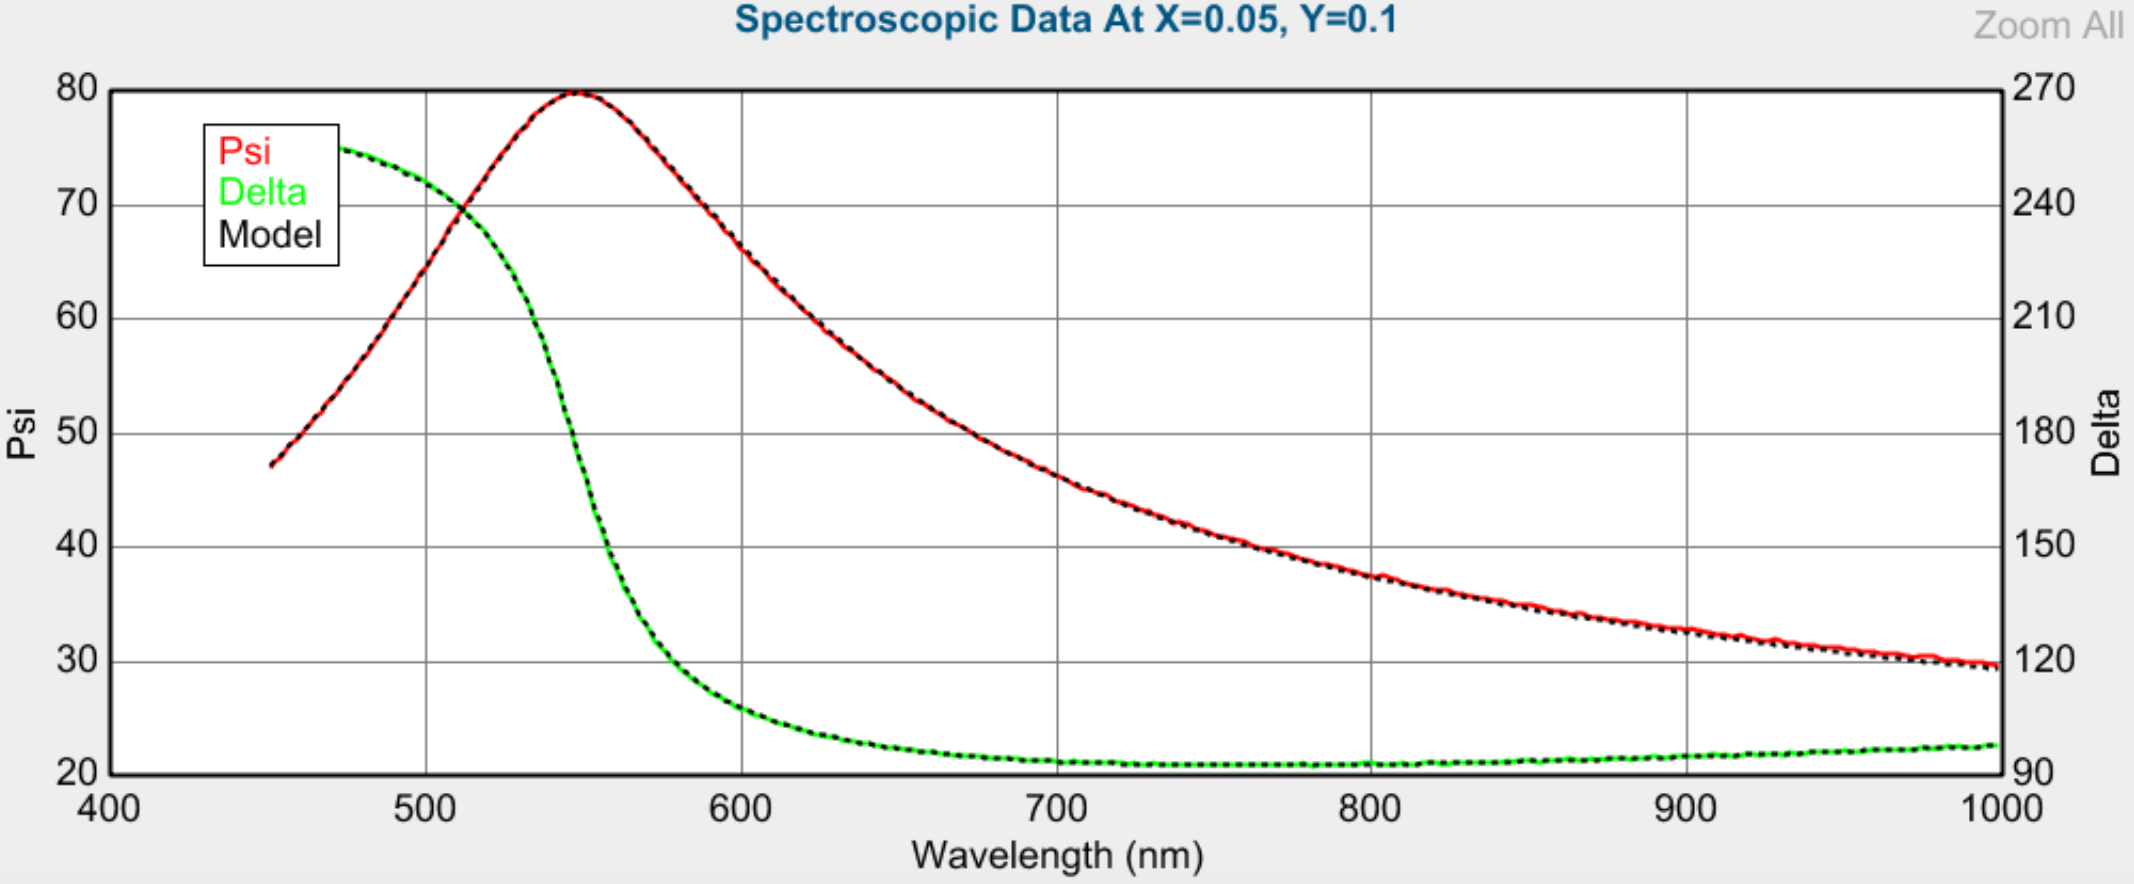
\includegraphics[scale=0.21]{Figures/SE_data_example.png}
% \includegraphics[scale=0.55]{Figures/diffraction_arc28.mps}
% \caption{Example of resist thickness measurement via SE}%{Example of a resist thickness measurement using SE with \textsc{Woollam}'s \textsc{CompleteEASE} software package, where $\Psi$ and $\Delta$ are shown as red and green curves with units given in degrees (\emph{top}). The sample is treated as a bilayer on a substrate where a film of native oxide is included between the resist and the silicon substrate, where both films are assumed to be transparent (\emph{bottom}). Using \cref{eq:Cauchy_index} for $\nu_2$ and tabulated data in \textsc{CompleteEASE} for $\nu_3$ and $\tilde{\nu}_4$, the thickness of resist in each dose square ($\tau_2$) could be measured with a fixed value of $\tau_3 = \SI{1.5}{\nm}$ for the native-oxide layer. Layers are not drawn to scale.}\label{fig:SE_example}
% \end{figure}
% \end{minipage}
%\end{frame}

%\begin{frame}{Grating Fabrication by TASTE}
%\begin{figure}
% \centering
% 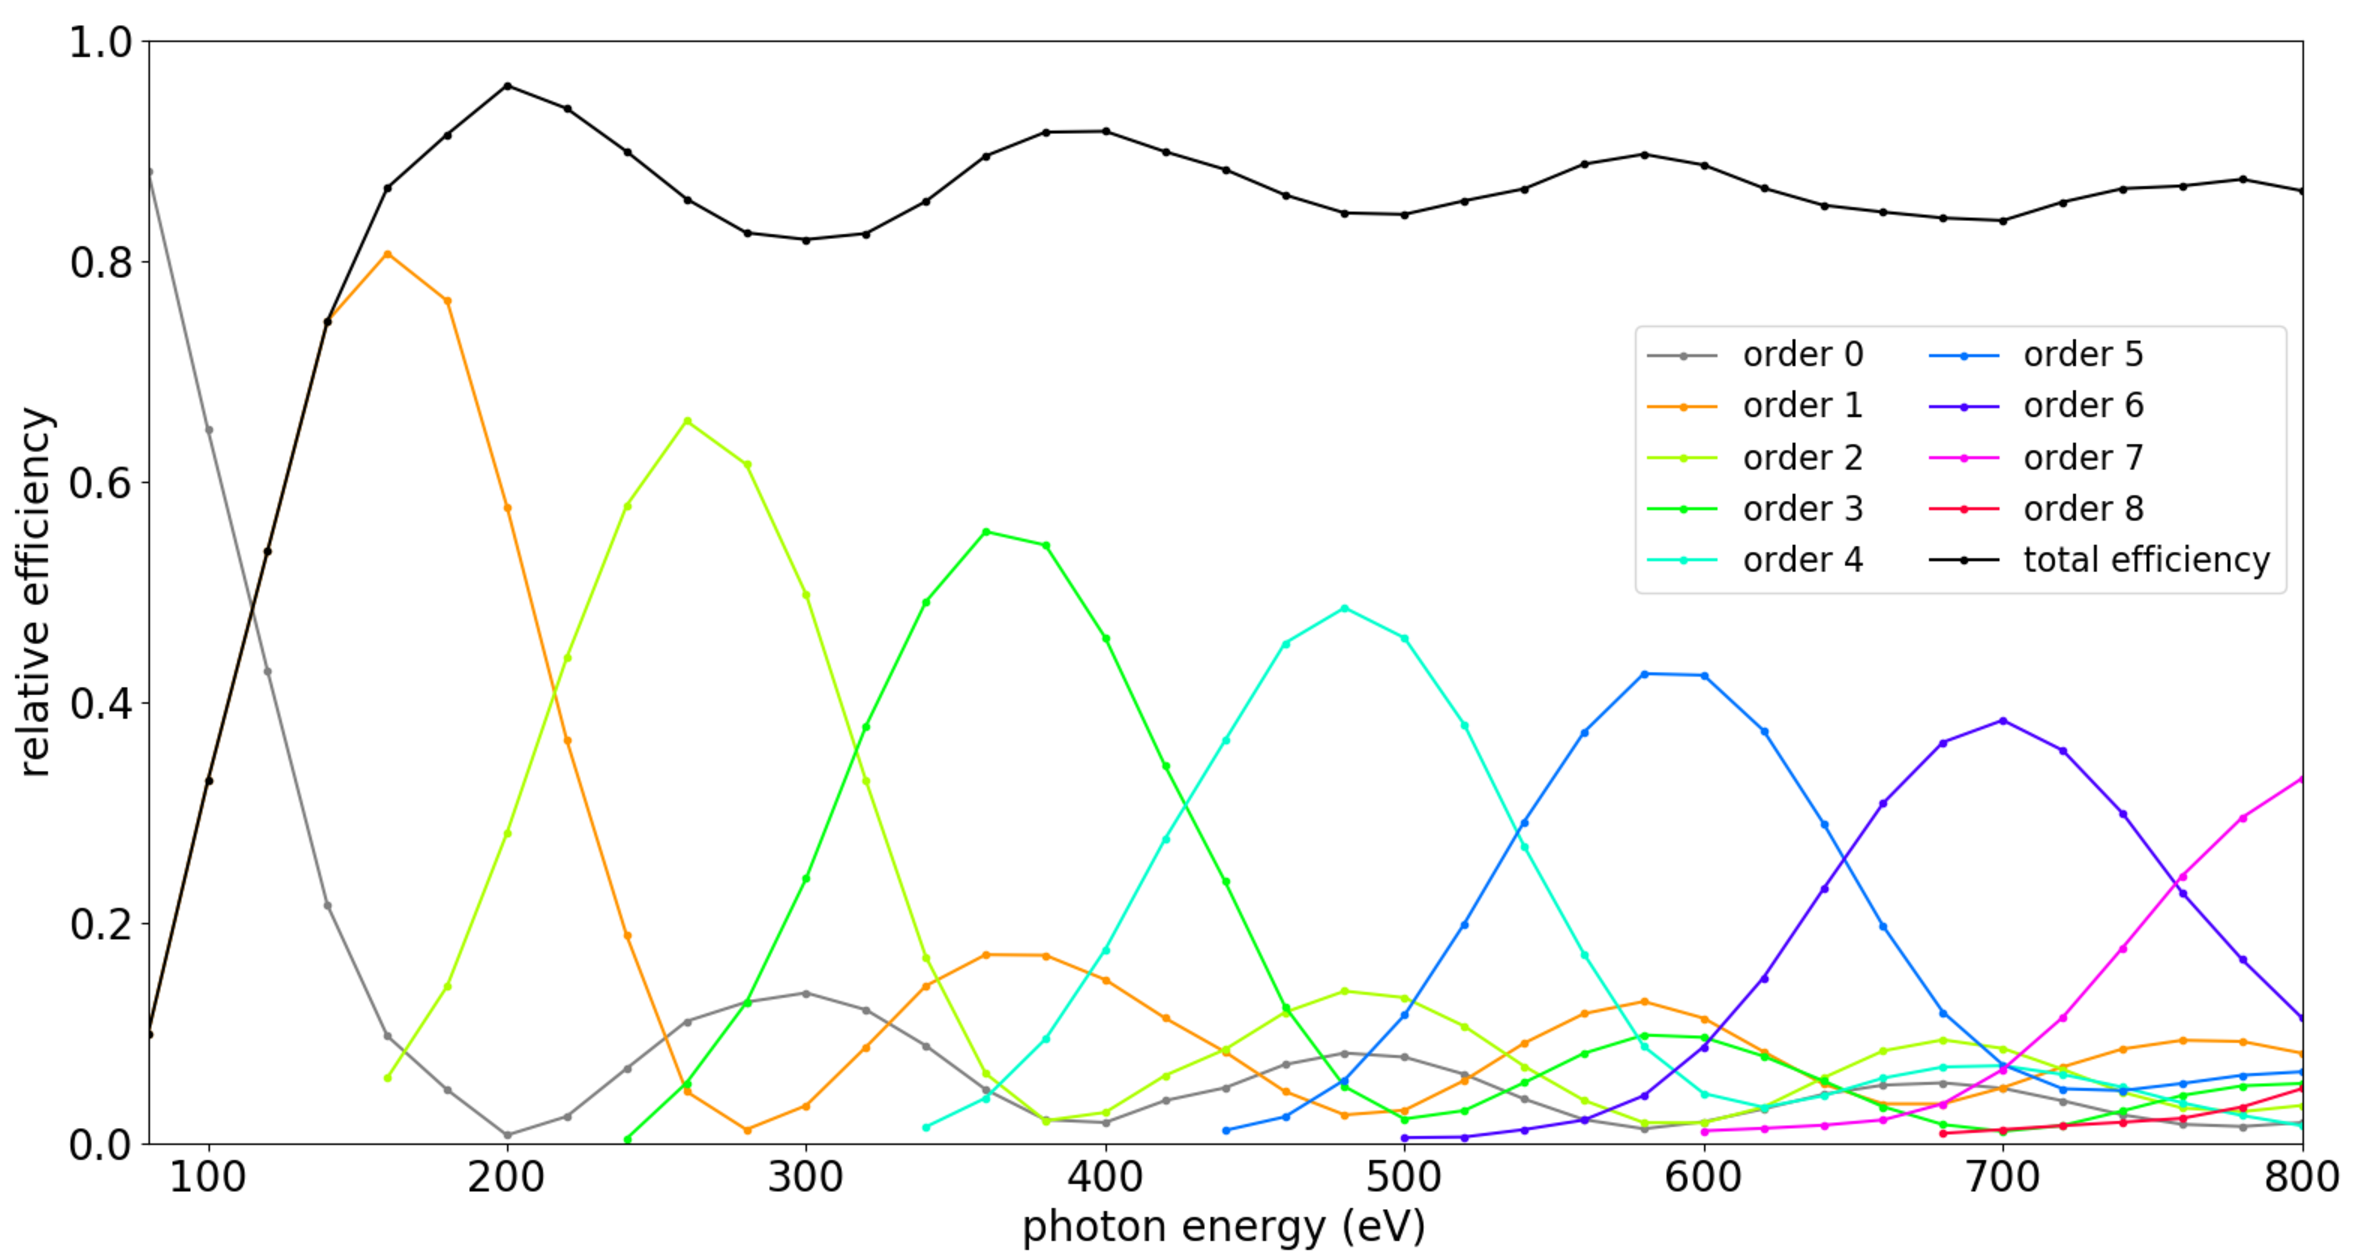
\includegraphics[scale=0.25]{Figures/relative_efficiency_fix.pdf}
% \caption{Relative diffraction efficiency calculated by dividing absolute diffraction efficiency by the Fresnel reflectivity of gold}%{Absolute diffraction efficiency data gathered at the ALS compared to the Fresnel reflectivity of gold, $\mathcal{R}_{F}$. Total diffraction efficiency below \SI{240}{\electronvolt} misses contributions from orders $n = \num{2}$ and $n = \num{3}$ on the order of a few percent.}\label{fig:abs_eff_taste}
% \end{figure} 
%\end{frame}

%\begin{frame}{Grating Fabrication by TASTE}
%begin{minipage}[t]{0.66\linewidth}
%\vspace{-2mm}
%\begin{figure}
% \centering
% 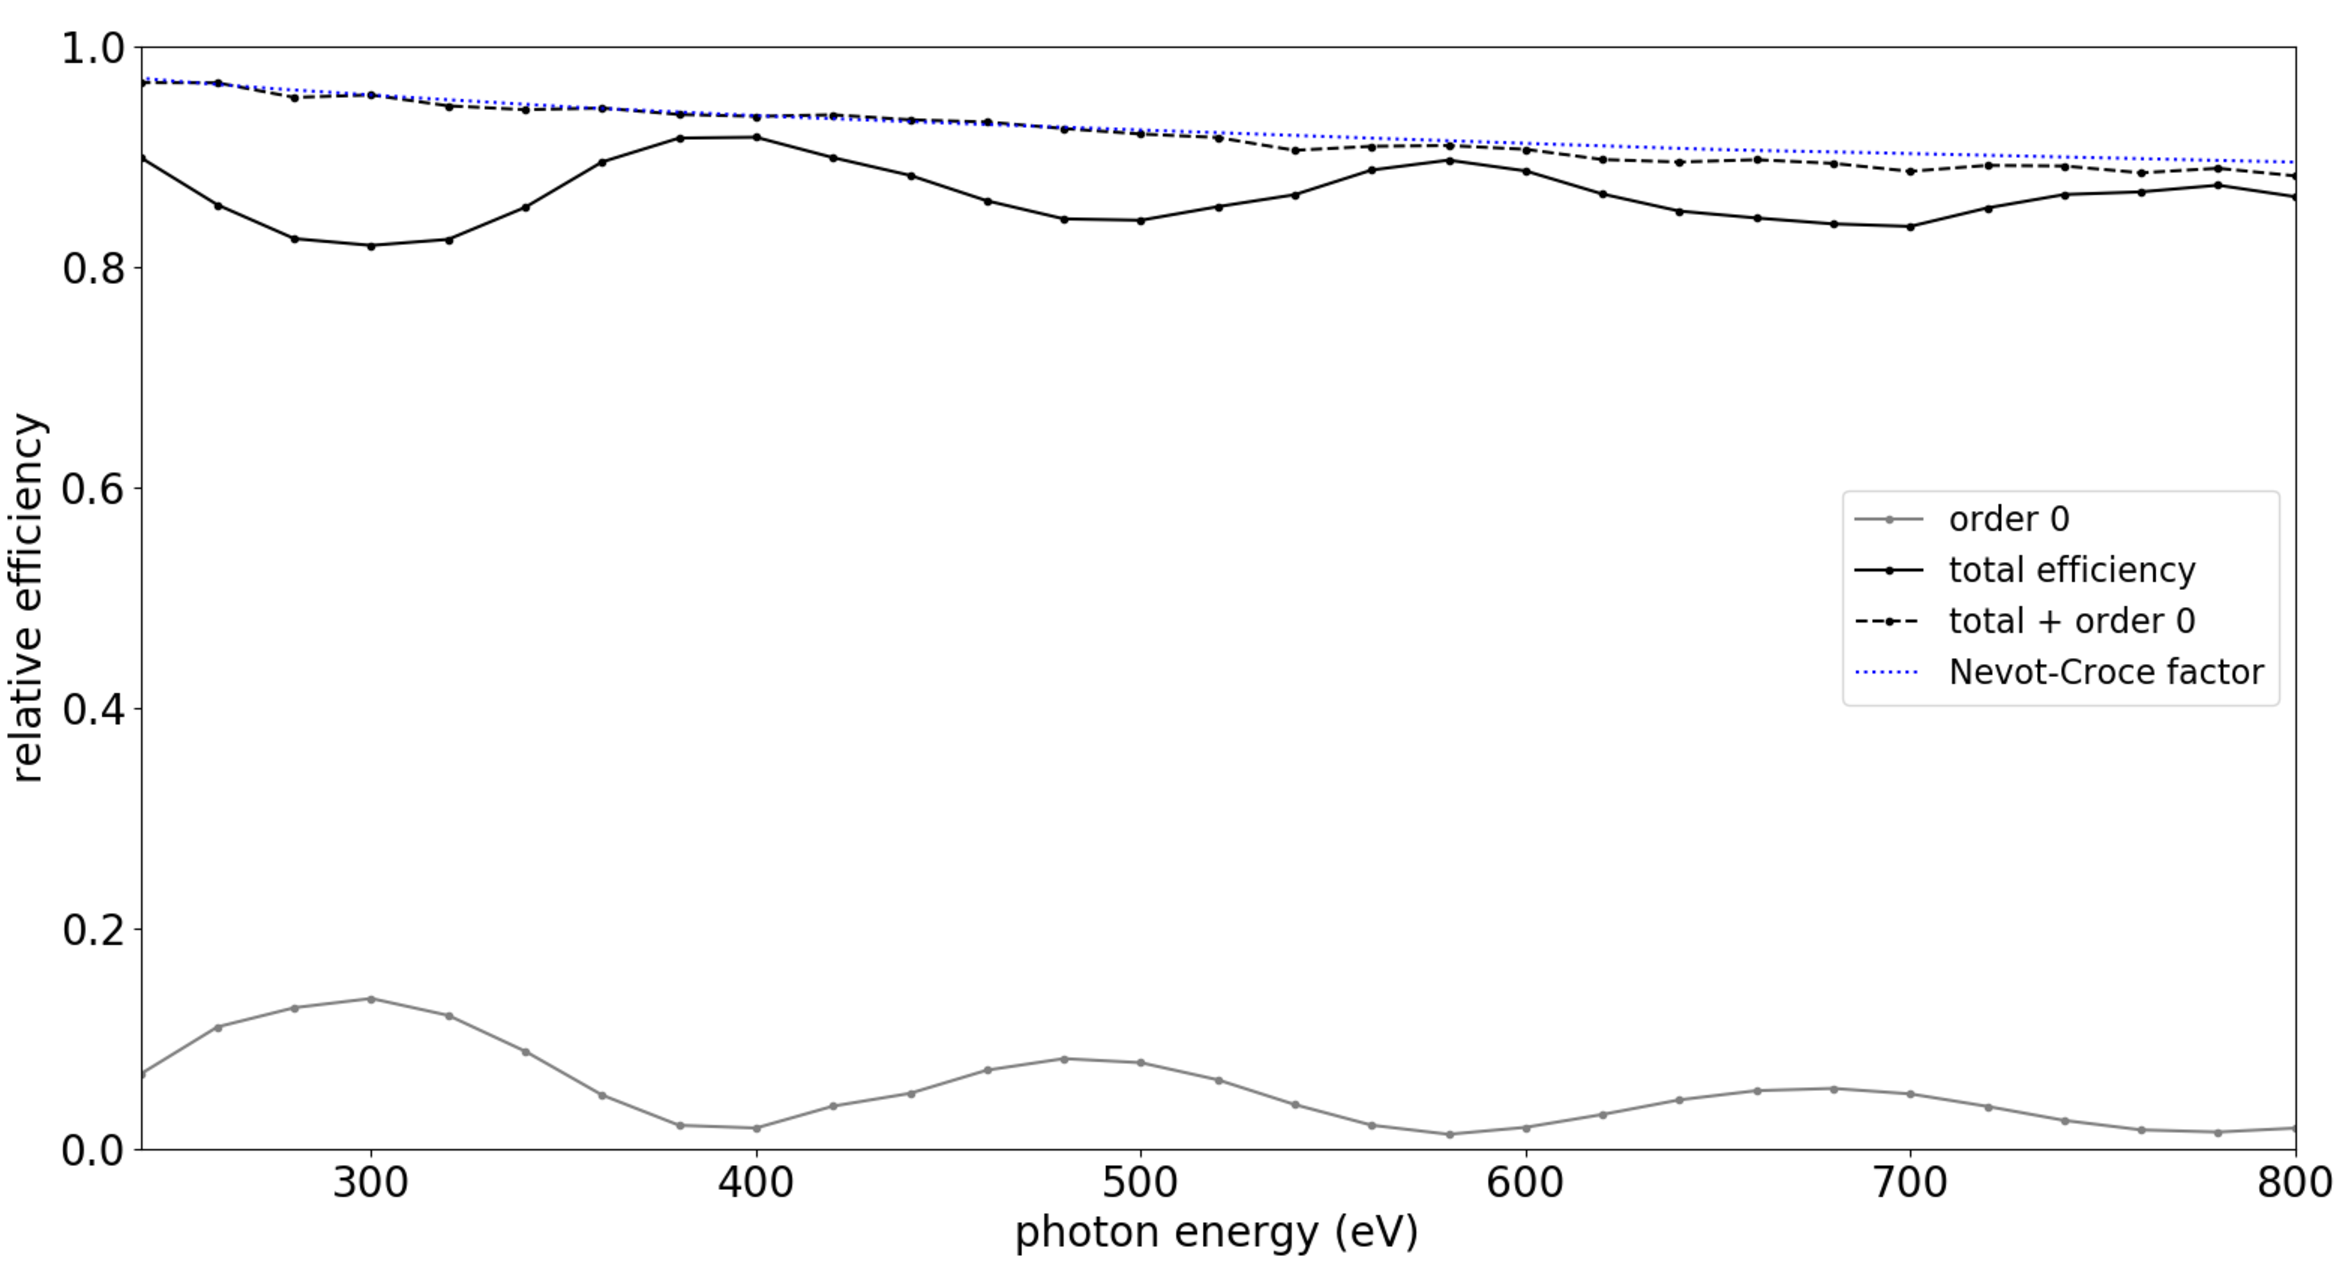
\includegraphics[scale=0.25]{Figures/total_eff_rough_factor.pdf}
% \caption{Total grating response plotted relative to $\mathcal{R}_F$ of gold, compared to Nevot-Croce factor for thick slab}%{Total grating response, defined as the sum of total diffraction efficiency and zero order, plotted relative to the reflectivity of gold. Overlaid is the Nevot-Croce factor [\emph{cf.\@} \cref{eq:nc_factor_taste}] for $\zeta = 1.73^{\circ}$ and $\sigma = \SI{1.5}{\nm}$ RMS, which indicates the theoretical specular reflectivity of a rough surface relative to Fresnel reflectivity.}\label{fig:rough_eff_taste}
% \end{figure}
% \vspace{-3mm}
 %  \centering {$\frac{\mathcal{R}_{NC}}{\mathcal{R}_F} = \norm{\mathrm{e}^{- 2 k_{\perp} \tilde{k}_{\perp} \sigma^2}}^2 = \mathrm{e}^{-4 k_0^2 \sin \left( \zeta \right) \Re \left[ \sqrt{\tilde{\nu}^2 (\omega) - \cos^2 \left( \zeta \right) } \right] \sigma^2}$}
 % \end{minipage}
 % \begin{minipage}[t]{0.33\linewidth}
 %\textbf{Facet roughness}
 %\begin{itemize}
 % \item \emph{Total relative response}: $\left( \mathscr{E}_{\text{tot}} + \mathscr{E}_0 \right) / \mathcal{R}_F$
 % \item \emph{Nevot-Croce (NC) factor} describes losses due to absorption in limit of small surface roughness
 % \item Data closely match NC factor with $\zeta \approx \gamma = 1.73^{\circ}$ and $\sigma \approx \SI{1.5}{\nm}$ RMS (via AFM)
 % \item Absorption due to facet roughness likely responsible for losses in grating response over $\SI{240}{\electronvolt} \leq \mathcal{E}%_{\gamma} \leq \SI{800}{\electronvolt}$
 % \begin{itemize}
 %   \item[$\square$] Diffuse scatter: $\lessapprox \SI{1}{\percent}$ for $\mathcal{E}_{\gamma} \gtrapprox \SI{600}{\electronvolt}$
 % \end{itemize}
  %\item $\lambda \gg 2 \pi \sigma \sin \left( \zeta \right) \approx \SI{0.3}{\nm}$
  %\item $\lambda \gg 2 \pi \ell_{\text{corr}} \sin^2 \left( \zeta \right) \approx \ell_{\text{corr}}/175$
% \end{itemize}
% \end{minipage}
%\end{frame}

%\begin{frame}{Grating Replication by SCIL}
%\begin{minipage}[t]{0.49\linewidth}
%\vspace{12mm}
%\begin{figure}
% \centering
% 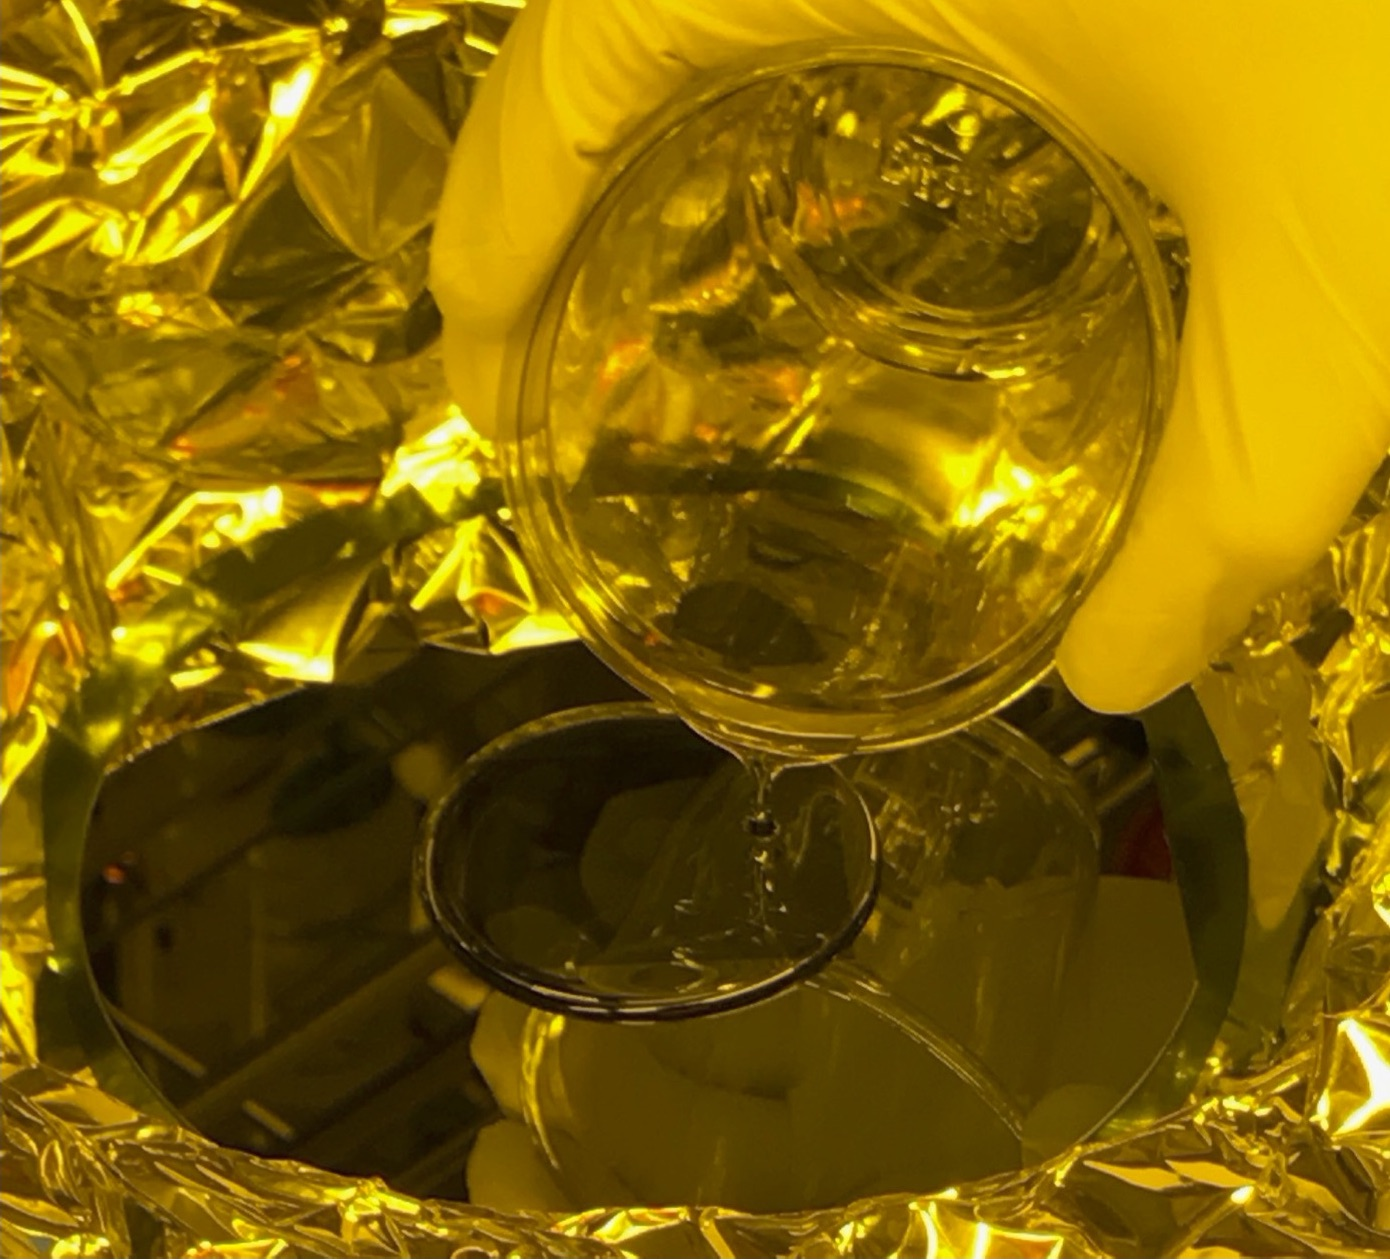
\includegraphics[scale=0.075]{Figures/SCIL_UPenn_spin_1.jpg}
% 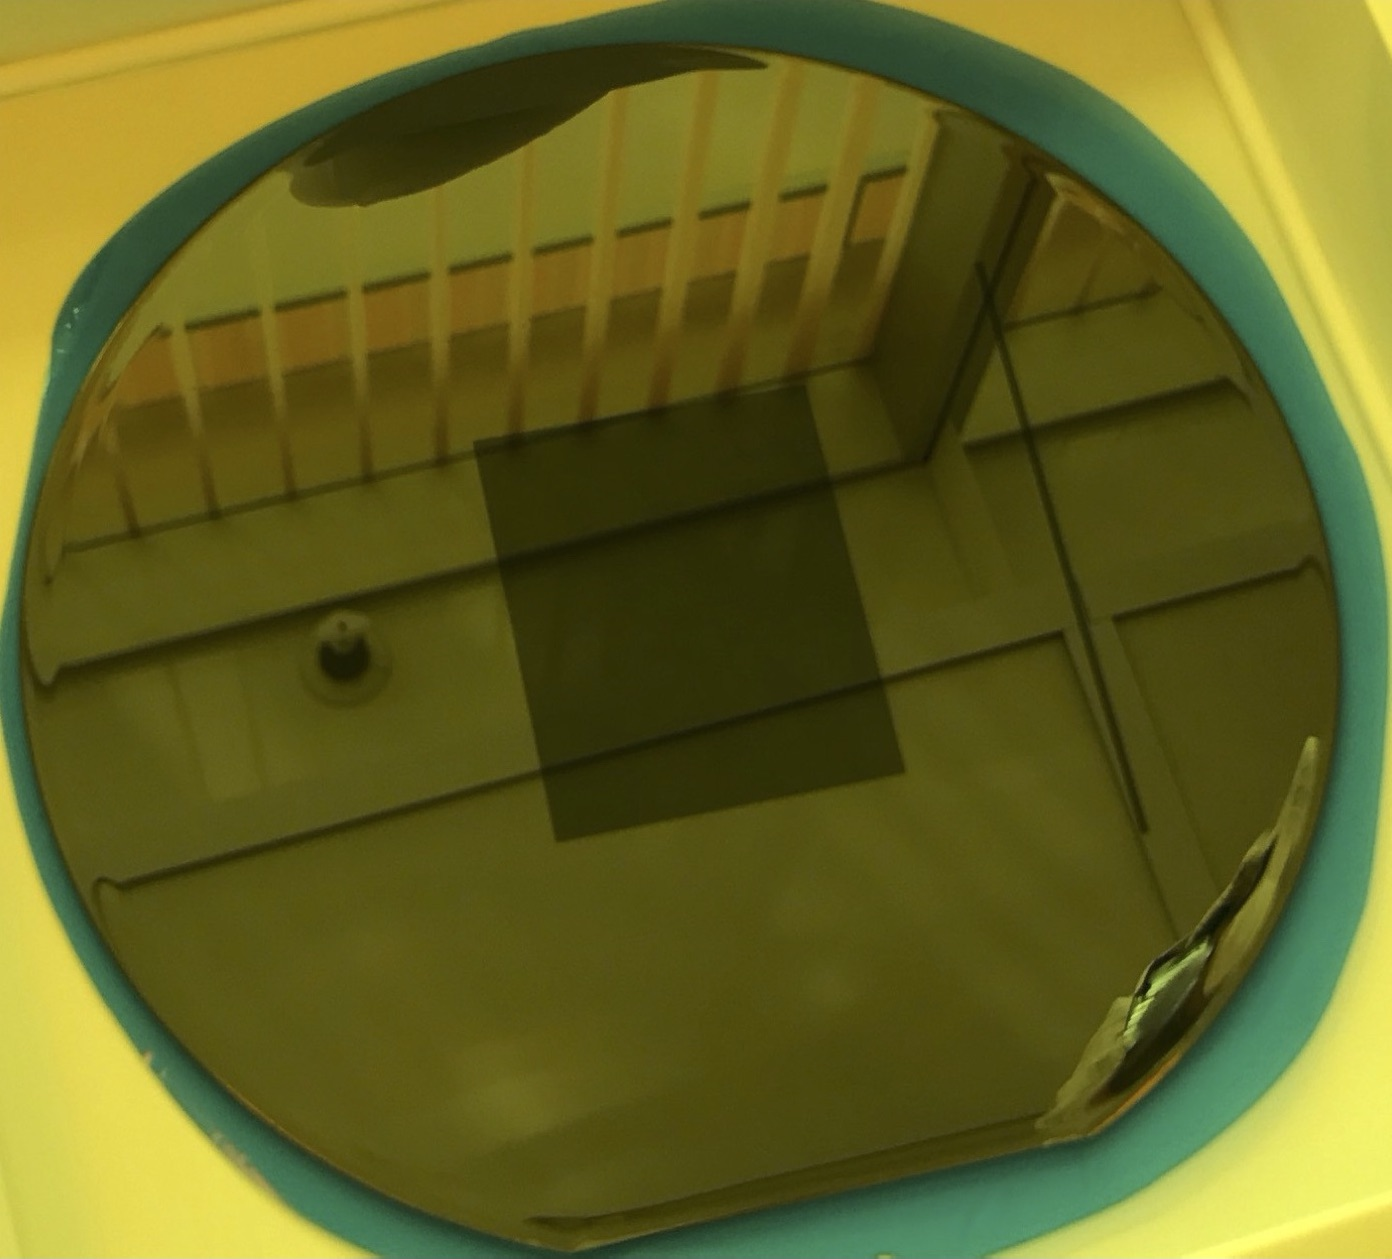
\includegraphics[scale=0.075]{Figures/SCIL_UPenn_spin_2.jpg}
% \caption{\SI{150}{\mm}-diameter, \ce{KOH}-etched silicon grating spin-coated with H-PDMS at the Quattrone Nanofabrication Facility (QNF), UPenn}%{A \SI{150}{\mm}-diameter silicon master spin-coated with H-PDMS at QNF. Due to the high viscosity of the material, a gradual spin acceleration must be used to achieve a uniform layer.}\label{fig:UPenn_spin}
% \end{figure}
%\end{minipage}
%\hfill
%\begin{minipage}[t]{0.49\linewidth}
%\vspace{-5mm}
%\begin{figure}
% \centering
% 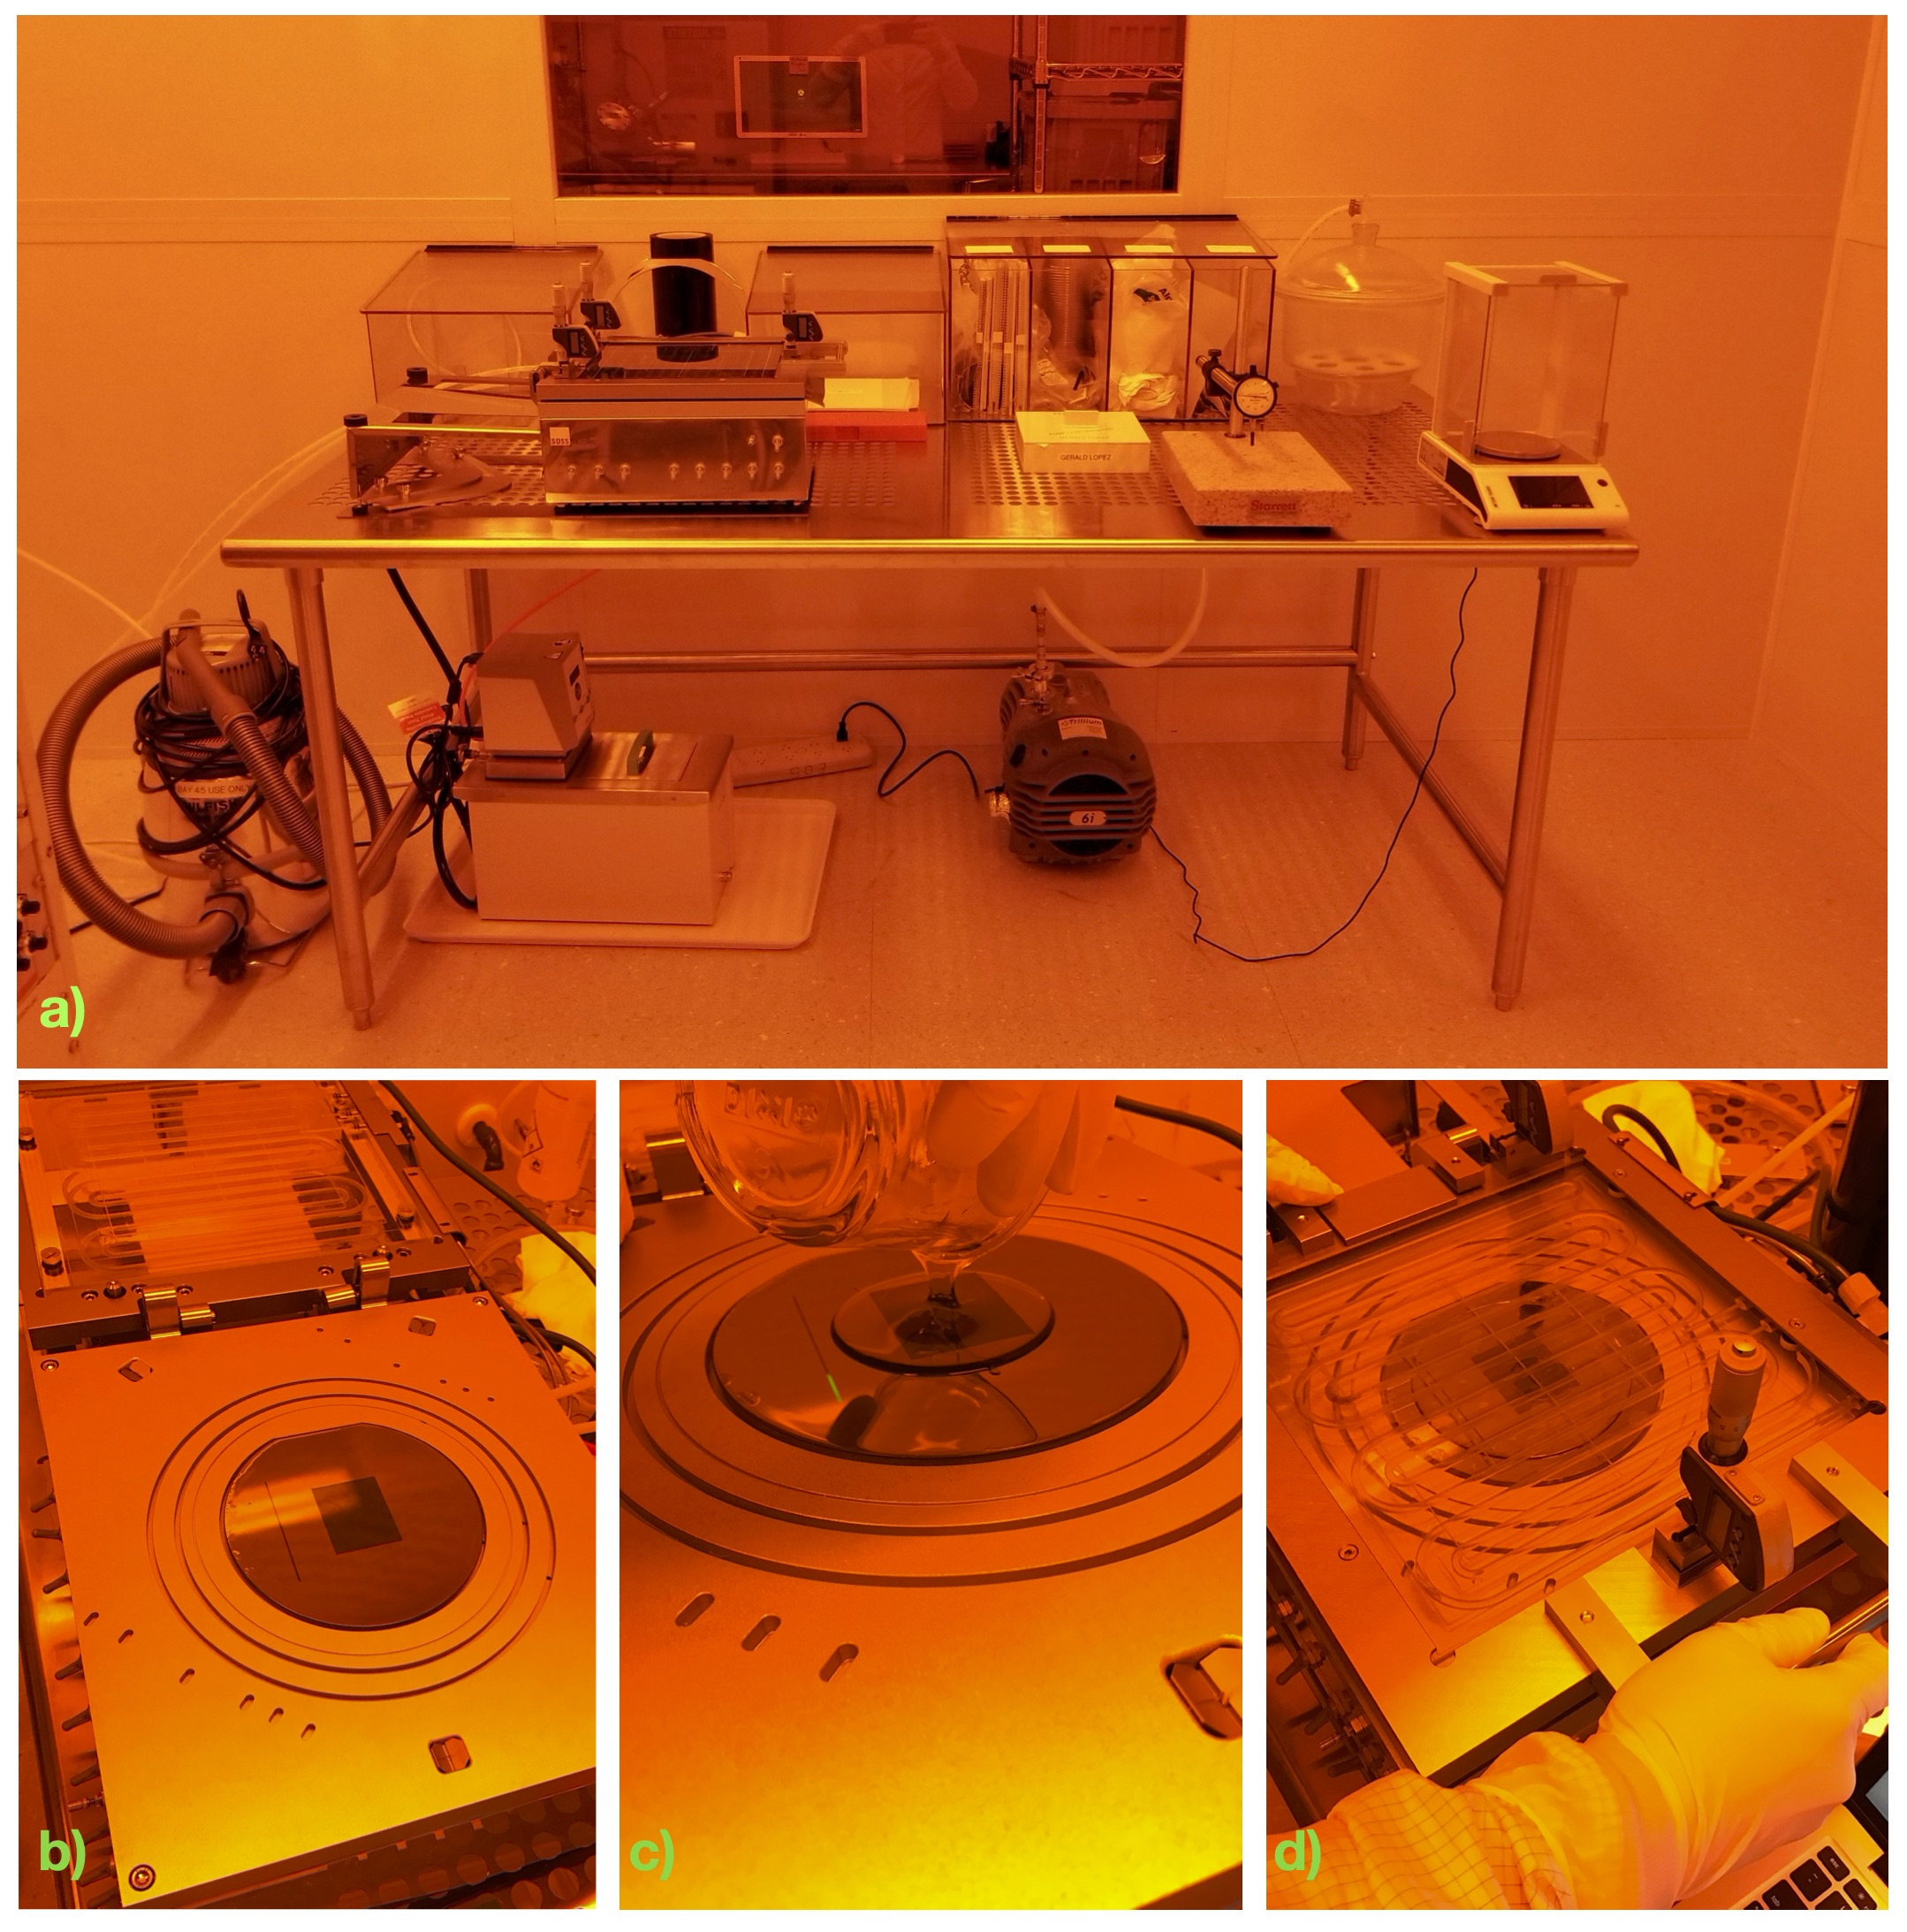
\includegraphics[scale=0.09]{Figures/SCIL_UPenn1.jpg}
% \vspace{-2mm}
% \caption{SCIL stamp construction at QNF}%{SCIL stamp construction at QNF: a) laboratory space featuring an MRT (\textsc{S{\"U}SS MicroTec}) and supporting equipment for surface heating and PDMS preparation, b) heated surfaces on the MRT for the silicon master and a flexible sheet of glass on the inside of the MRT lid, c) PDMS is poured over the surface of the silicon master, d) the MRT lid is closed and the PDMS is cured at \SI{50}{\celsius}.}\label{fig:UPenn1}
% \end{figure}
% \end{minipage}
%\end{frame}

%\begin{frame}{Grating Replication by SCIL}
% \begin{minipage}[t]{0.50\linewidth}
% \textbf{SCIL for x-ray reflection gratings}
% \begin{itemize}
%  \item Use \ce{KOH}-etched silicon master (Miles, et al.~2018)
%  \begin{itemize}
%    \item[$\square$] $\delta = 30.0 \pm 0.8^{\circ}$ under AFM
%    \item[$\square$] Surface-treat for anti-stiction
%  \end{itemize}
%  \item Construct composite SCIL stamp
%    \begin{itemize}
%    \item[$\square$] Spin-coat, bake X-PDMS over surface-treated silicon master
%    \item[$\square$] Use round sheet of glass for stamp substrate
%  \end{itemize}
%  \item Construct inverted stamp
%    \begin{itemize}
%    \item[$\square$] Imprints should emulate UV-NIL replicas %(sharp apex)
%    \item[$\square$] Repeat steps using first stamp as template
%  \end{itemize}
% \end{itemize}
 %\hspace{-2mm}
% \begin{figure}
% \centering
% 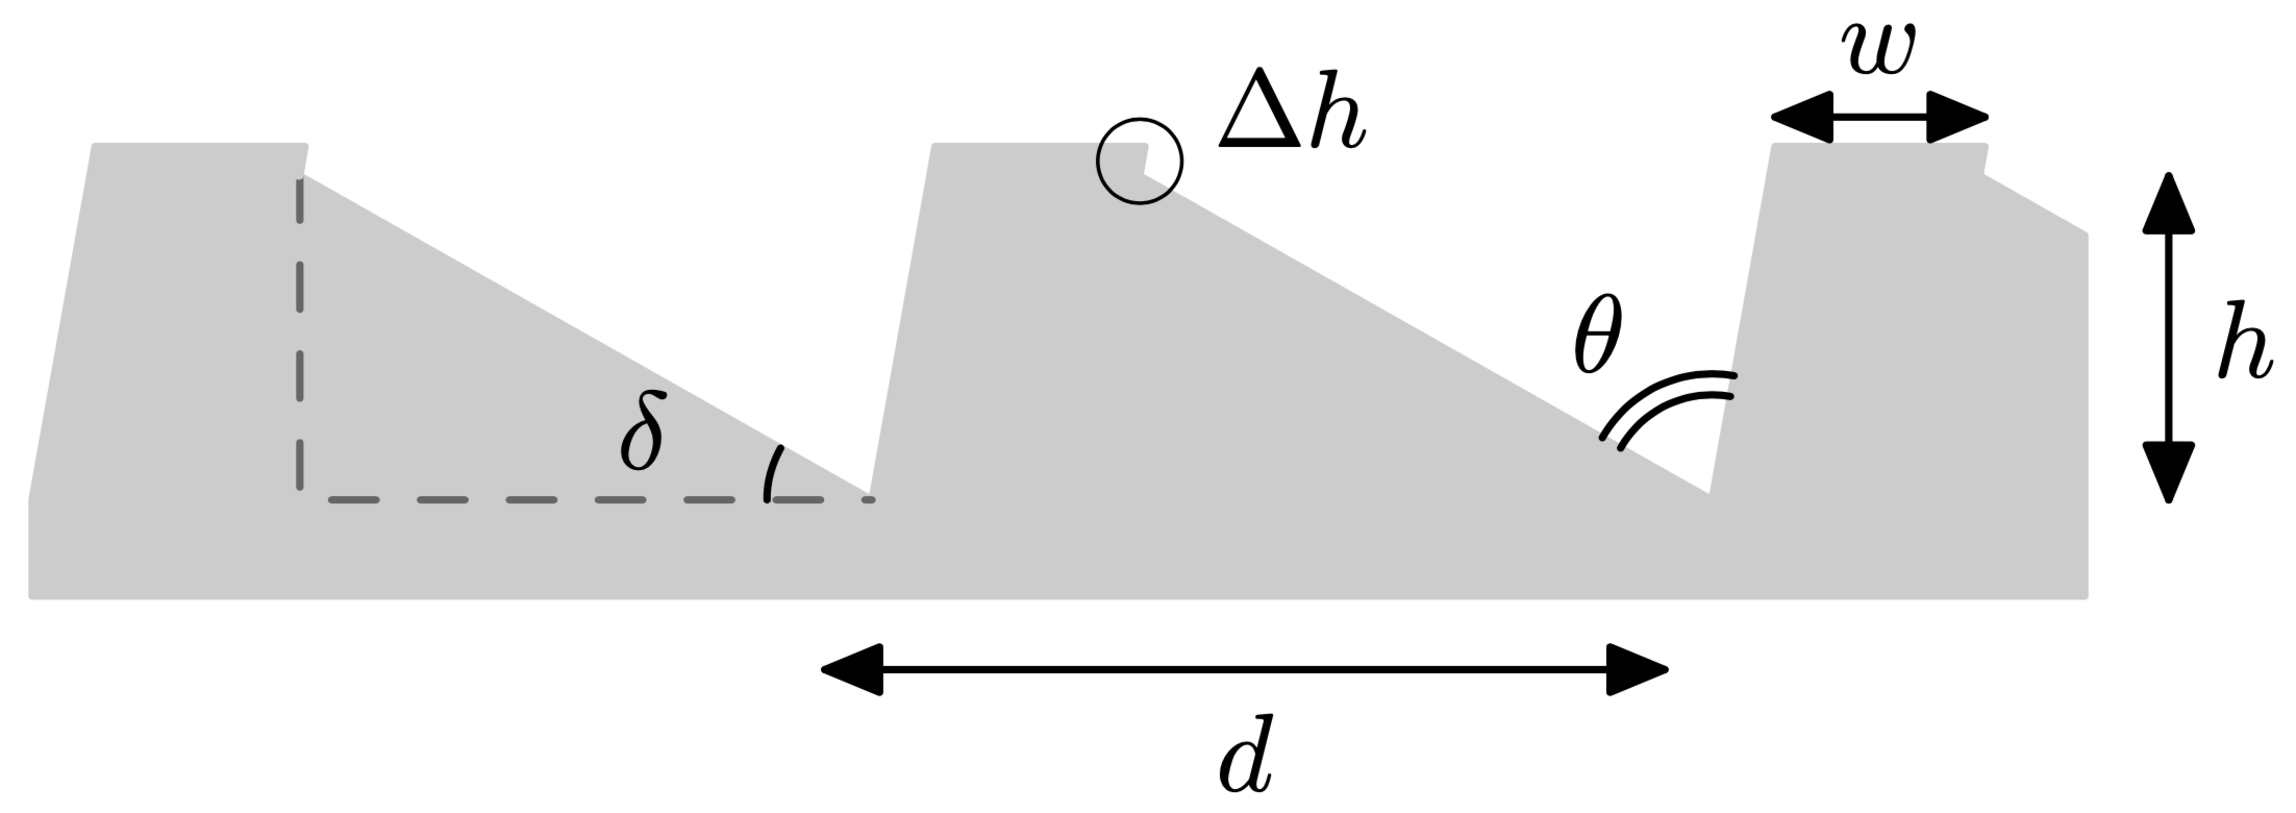
\includegraphics[scale=0.15]{Figures/master_grating_fab_final.pdf}
% \vspace{-2mm}
% \caption{Illustration of \ce{KOH}-etched silicon master}%{Illustration of the \ce{KOH}-etched silicon master surface profile from \cref{fig:master_fab} with $\delta = 29.5^{\circ}$ as the nominal blaze angle and $\theta \approx 70.5^{\circ}$ defined by the intersection of exposed $\{ 111 \}$ planes. At a groove spacing of $d \lessapprox \SI{160}{\nm}$, the flat-top regions have widths $w \gtrapprox \SI{30}{\nm}$ as a result of the etch undercut while the groove depth is $\SI{65}{\nm} \lessapprox h \lessapprox \SI{70}{\nm}$ by \cref{eq:groove_depth}. Indicated by the circle, the indented portion of the etched topography cannot be described with a functional form for the diffraction-efficiency analysis in \cref{sec:discussion_scil}.}\label{fig:master_grating_profile} 
% \end{figure}
% \end{minipage}
 %\vspace{-4mm}
%\begin{minipage}[t]{0.46\linewidth}
% \vspace{-2mm}
%\begin{figure}
% \centering
 %\hspace{-6mm}
 %\vspace{-1mm}
% 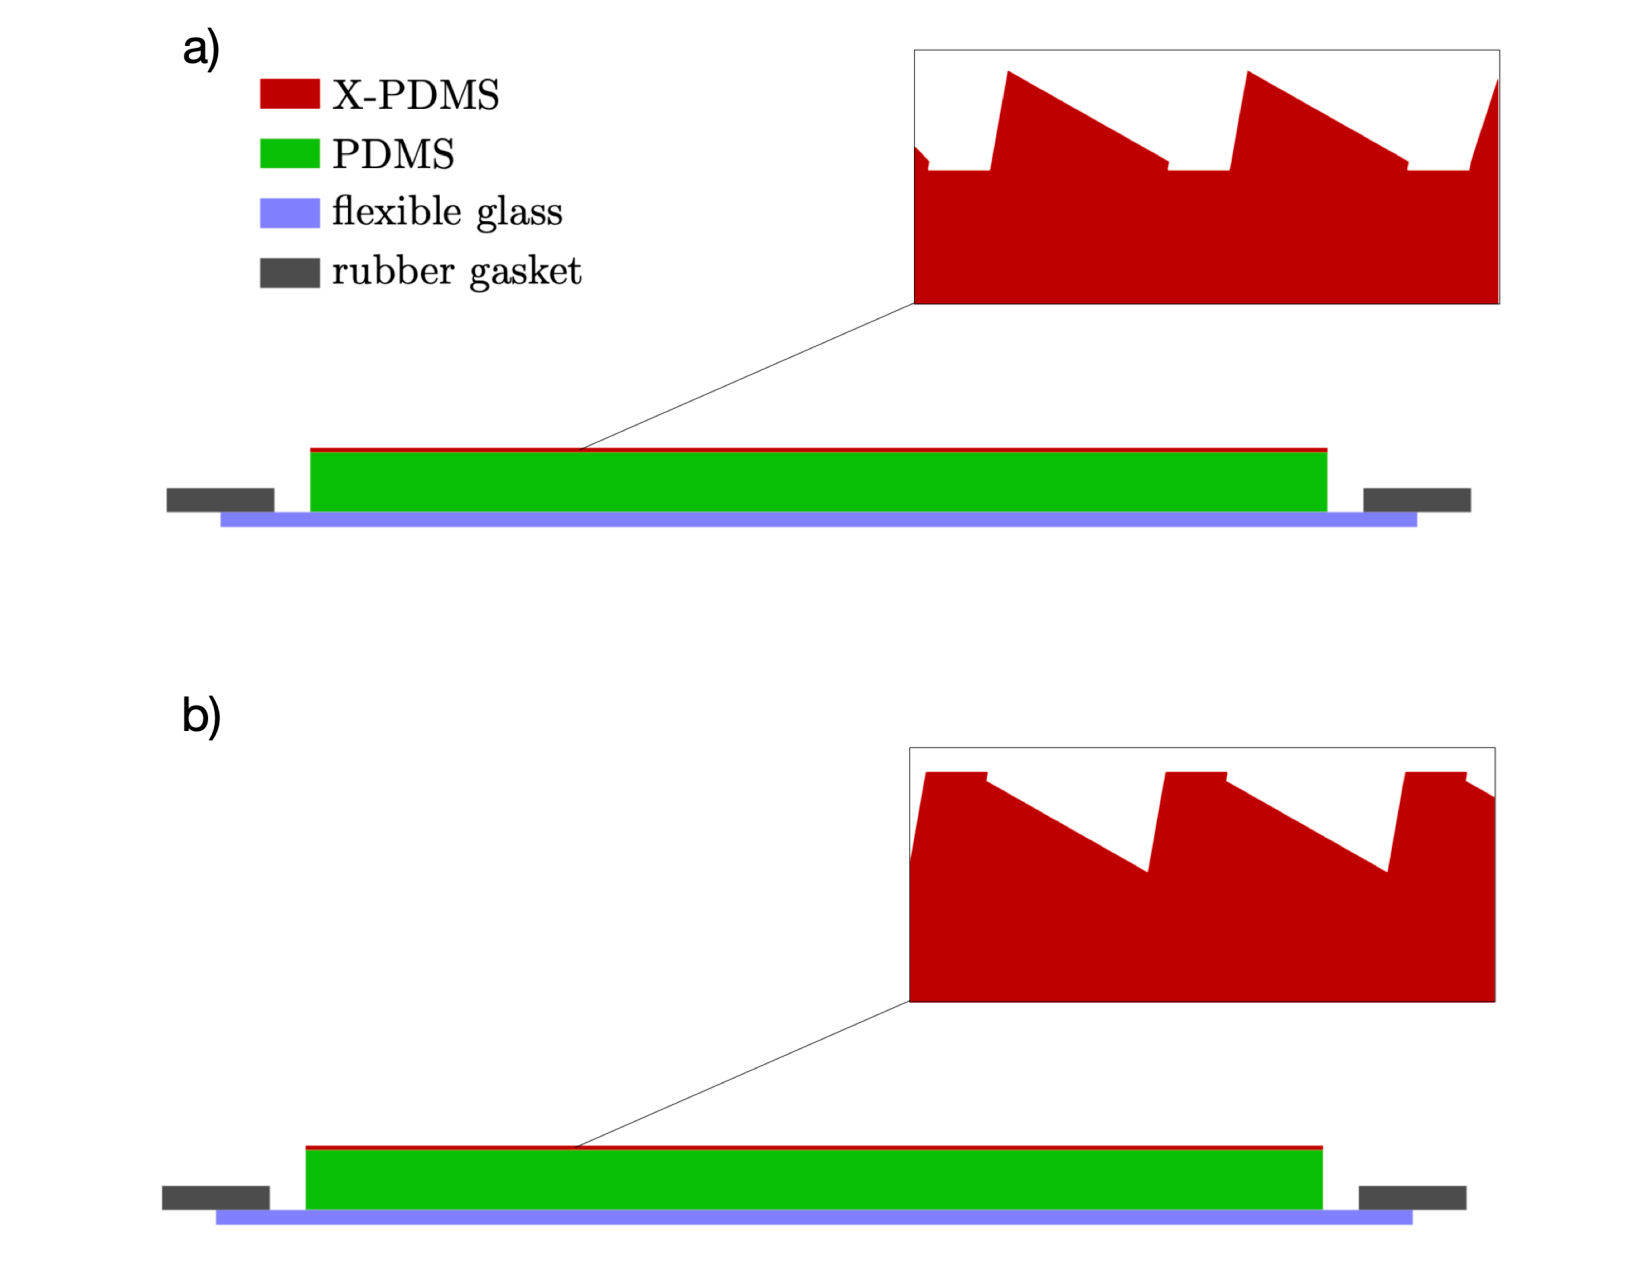
\includegraphics[scale=0.28]{Figures/SCIL_stamp.pdf}
% \vspace{-3mm}
% \caption{Schematic for SCIL composite stamps of two varieties: a) \emph{non-inverted}, b) \emph{inverted}}%{Schematic for SCIL composite stamps of two varieties: a) an initial stamp featuring an inverted topography molded directly from the silicon master and b) a second stamp  featuring a topography similar to the master grating, which was molded using the first stamp as a master template. In either case, grating grooves are carried in a layer of X-PDMS tens of \si{\um} thick that sits on a \SI{200}{\mm}-diameter, flexible glass sheet buffered by a $\gtrapprox \SI{0.5}{\mm}$-thick layer of soft PDMS. A rubber gasket can be attached for use with the pneumatic-based SCIL wafer-scale imprint method. This illustration neglects slight rounding that can occur in sharp corners under the influence of surface tension in X-PDMS.}\label{fig:scil_stamps}
% \end{figure}
% \end{minipage}
%\end{frame}

%\begin{frame}{Grating Replication by SCIL}
%\begin{figure}
% \centering
% 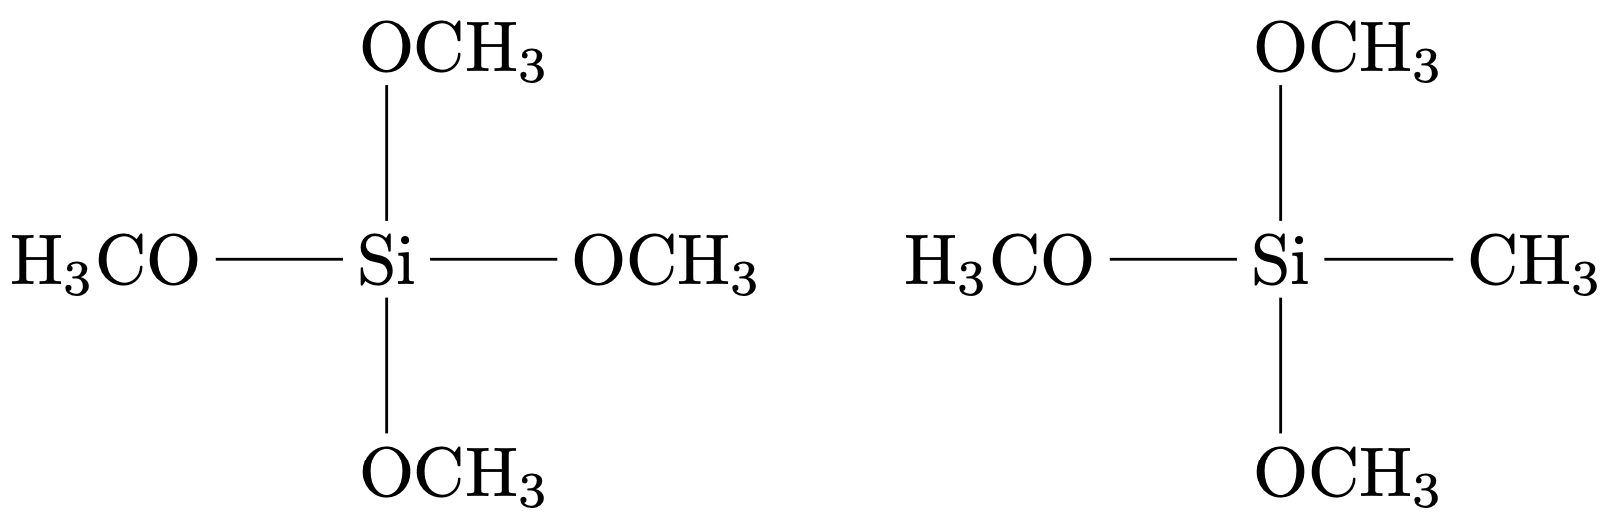
\includegraphics[scale=0.2]{Figures/precursors.png}
 %\caption{Structural formula of the sol-gel precursors used for \textsc{NanoGlass} imprint resist in SCIL}%{Structural formula of the sol-gel precursors used for \textsc{NanoGlass} imprint resist: TMOS (\emph{left}; fully inorganic with four methoxy groups) and MTMS (\emph{right}; organically modified with three methoxy groups and one methyl group).}\label{fig:precursors}
% \end{figure}
%\vspace{-2mm}
%These precursors react to form a gel, and ultimately a solid silica-like network, along with alcohols and water left as reaction products \cite{Verschuuren10,Verschuuren19}. 
%Briefly, methoxy groups (\emph{i.e.}, \ce{-O-CH3}) bonded to silicon in TMOS (\emph{left} and MTMS (\emph{right} undergo hydrolysis so that they are replaced with hydroxyl groups (\emph{i.e.}, \ce{-OH}): 
%\begin{equation}
% \ce{Si-(O-CH3)} + \ce{H2O} \longrightarrow \ce{Si-OH} + \ce{HO-CH3} , 
% \end{equation}
%where methanol (\emph{i.e.}, \ce{HO-CH3}) is produced as a reaction product. 
%Hydrolyzed silicon sites can then react with one another to form a siloxane bond with the release of water: 
%\begin{equation}
% \ce{Si-OH} + \ce{HO-Si} \longrightarrow \ce{Si-O-Si} + \ce{H2O} 
% \end{equation}
%and as these condensation reactions continue, a silica-like material network is formed. 
%This sol-gel process carries out over the course of \SI{15}{\minute} at room temperature while reaction products and trapped air diffuse into the stamp, leaving solidified resist molded to the inverse of the stamp topography after stamp separation. 
%\end{frame}

% The [plain] causes the headlines, footlines, and sidebars 
% to be suppressed. Useful for showing large pictures
%\begin{frame}[plain]
%  \begin{center}
%    This is a plain frame.\\
%    Use it to display full page images.
%    \end{center}
%\end{frame}

%\begin{frame}
% \centering
% \frametitle{Flux}
% \framesubtitle{license}
% Flux is licensed under GNU General Public License v3.\\[0.3cm]
%  \centering\textbf{http://www.gnu.org/licenses}\\[0.3cm]
%Inspired by \textbf{Metropolis} theme from Matthias Vogelgesang.\\
%https://github.com/matze/mtheme 
 
%\end{frame}

\end{document}